\documentclass[aspectratio=43]{beamer}
\usepackage[T1]{fontenc}
\usepackage[utf8]{inputenc}
\usepackage[english]{babel}
\usepackage{bm}
\usepackage{subfig}
\usepackage{pgfplots}
\pgfplotsset{compat=newest}

\usepackage{booktabs}
\usepackage{siunitx}
\newcommand{\Ex}{\mathbb{E}}
\newcommand{\Var}{\mathbb{V}\mathrm{ar}}
\newcommand{\Prob}{\mathbb{P}}
\DeclareMathOperator*{\argmin}{arg\,min}
\DeclareMathOperator*{\argmax}{arg\,max}
\usepackage{multicol}
%\usepackage{pgfpages}
%\setbeameroption{show notes}
%\setbeameroption{show notes on second screen=right}
% Latin Modern
\usepackage{lmodern}

% Verdana font type
%\usepackage{verdana}
% Helvetica
%\usepackage{helvet}
% Times (text and math)
%\usepackage{newtx, newtxmath}
\graphicspath{{../Figures/}}
\usetheme[department=aqua]{DTU}

\title[Robust estimation of bottom friction]{Robust Estimation of bottom friction \\ \textit{Parameter control in the presence of uncertainties}}
\author{\textsc{Victor Trappler} \\ s151431}
\institute{Master Thesis Defence}
\date{\today}
	
\newcommand{\tabitem}{{\color{dtured}$\bullet$} }
\setcounter{tocdepth}{1}

\begin{document}
\frame{
	\maketitle
	\note{Hello ! Name, reason}
}

\section{Introduction}
\subsection{AIRSEA team}
\frame{
\frametitle{The AIRSEA team, Grenoble, FRANCE}
\begin{figure}[!h]
  \centering
  \subfloat{
\includegraphics[width = 0.4\textwidth]{INRIA_SCIENTIFIQUE_UK_CMJN}}
  \subfloat{
\includegraphics[width = 0.4\textwidth]{ljk}}
\end{figure}
\pause
\begin{itemize}
\item Modelling Oceanic and Atmospheric flows: \alert<3->{parametrization} and  coupling of the equations
\item Model reduction, multiscale algorithms
\item High-performance computing
\item \alert<3->{Dealing with uncertainties}
\end{itemize}
}
\subsection{Context and scope of the project}
\frame{
%\frametitle{Parameter control and uncertainties}
%\begin{itemize} \item Subgrid phenomena need \emph{parametrization}\pause
%
%\item \emph{Uncertainties} arise from: 
%\begin{itemize}
%\item physical model
%\item numerical model
%\item observations error 
%\end{itemize}
%\end{itemize}
\begin{center}
\begin{tikzpicture}
\usetikzlibrary{decorations.pathmorphing}

\definecolor{copper}{rgb}{0.69, 0.25, 0.21}
\definecolor{tin}{rgb}{0.7, 0.7, 0.7}

\tikzset{
  rugous1/.style = {black, thick,
    decoration={random steps,segment length=0.05cm,amplitude=.1cm}
  },
}
\tikzset{
  rugous2/.style = {black, thick,
    decoration={random steps,segment length=0.2cm,amplitude=.05cm}
  },
}
\tikzset{
  rugous3/.style = {black, thick,
    decoration={random steps,segment length=0.2cm,amplitude=.15cm}
  },
}

\filldraw [fill = blue!30]
   plot [samples = 100,domain = -5:5] (\x, {0.5*sin(\x r) + 2} )
-- plot [samples = 100,domain = 5:-5] (\x, {0.3*sin(\x/1.5 r)+0.5})
-- cycle;

\filldraw[fill = gray!30, draw = white]
   plot [samples = 100,domain = -5:5] (\x, {0.3*sin(\x/1.5 r)+0.5})
-- plot [samples = 100,domain = 5:-5] (\x, 0)
-- cycle;

\draw[rugous1, decorate](-5,0.52) -- (-2.3,0.2);
\draw[rugous2, decorate](-2.3,0.2) -- (2.4,0.8);
\draw[rugous3, decorate](2.4,0.8) -- (5,0.5);

\draw[->] (-5,0) -- (5,0);
\draw (0,0) node[below] {$x$};



\draw[->] (-5,0) -- (-5,3);

\draw[->] (0,0.5) -- (0,2);
\draw (0, 1.25) node[left] {$h(x,t)$} ;
\draw (0,0) node[below] {$x$};
\draw[->] (2,0) -- (2,{0.3*sin(2/1.5 r)+0.5});
\draw (2, 0.3) node[right] {$Z(x)$} ;
\draw[->] (1,0) -- (1,{0.5*sin(1 r)+2});
\draw (1, 1.3) node[right] {$H(x,t)$} ;
\end{tikzpicture}
\end{center}
}
\frame{
	\frametitle{Outline}
	\tableofcontents
}
\setcounter{tocdepth}{2}
\section{Deterministic Framework}
\frame{
\frametitle{Deterministic Framework}
\tableofcontents[
    currentsubsection, 
    sectionstyle=show/shaded, 
    subsectionstyle=show/hide,
    hideothersubsections
    ]
}
\subsection{The 1D Shallow Water Equations}
\frame{
\frametitle{The 1D Shallow Water Equations}
	\begin{block}{1D-SWE}
		\begin{align}
			&\partial_t \alert<1>{h} + \partial_x \alert<1>{q} = 0 \tag{Conservation}\\
			&\partial_t \alert<1>{q} + \partial_x \left(\frac{\alert<1>{q}^2}{\alert<1>{h}} + \frac{1}{2}g\alert<1>{h}^2\right) = -g\alert<1>{h} \partial_x Z - S \tag{Momentum}
		\end{align}
	\end{block}
	\pause
	\begin{block}{Quadratic Friction}
	\begin{equation*}
		S = - \alert<2>K|q|qh^{-\eta},\quad \eta = 7/3
	\end{equation*}
\end{block}
$K$: control parameter. Either a scalar value or a vector
}
\frame{
\frametitle{Computer code}
\begin{itemize}
	\item 1D Shallow water equations
	\begin{itemize}
		\item $K$: Bottom friction
		\item Boundary conditions (considered fixed and known)
	\end{itemize}
	\item Output $W(K)$:\\ $W_i^n(K) = [h_i^n(K) \quad q_i^n(K)]^T$, for $0 \leq i \leq N_x$ and $0 \leq n \leq N_t$
\end{itemize}
\begin{figure}[!b]
\centering
\only<1>{\tikzstyle{block} = [rectangle, draw, fill=blue!20, 
     text centered, minimum width=1cm]

\tikzstyle{block2} = [rectangle, draw, fill=green!20, 
     text centered, rounded corners, minimum width=1cm]

\tikzstyle{LHS}=[rectangle, draw, text centered]

\begin{tikzpicture}[node distance=3cm]

\node [align = center] at (0,0) (input) {Control variable \\$K \in \mathcal{K}$};
%\node [align = center] at (4,1.5) (envir) {Environmental variables \\$\bm{u} \in \mathcal{U}$ fixed};
\node [align = center] at (4,1.5) (envir) {Environmental variables \\$\bm{x}_e \in \mathbb{X}$ fixed};

\node[block] at (4,0)(code){Direct Simulation};

\node[align = center] at (8,0) (output) {$W(K)$}; %\\ $\Rightarrow j(K)$};

\draw[->] (input) -- (code);
\draw[->] (envir) -- (code);
\draw[->] (code) -- (output);

\end{tikzpicture}}
%\only<2>{\usetikzlibrary{positioning}
% \tikzstyle{block} = [rectangle, draw, fill=blue!30, 
%     text centered, minimum width=3em] 
 \tikzstyle{block} = [rectangle, draw, fill=blkcol, 
      text centered, minimum width=3em]

\tikzstyle{block2} = [rectangle, draw, fill=blkcol2, 
     text centered, rounded corners, minimum width=3em]

% \tikzstyle{block2} = [rectangle, draw, fill=blkcol2, 
%      text centered, rounded corners, minimum width=3em]

\tikzstyle{LHS}=[rectangle, draw, text centered]

\begin{tikzpicture}

%\node [align = center] at (0,0) (input) {Control variable \\$\mathbf{k} \in \mathbb{K}$};
\node [align = center] at (0,0) (input) {Control variable \\$\bm{k} \in \mathbb{K}$};
\node[block] at (4,0) (code){Direct Simulation};
%\node [align = center, above =of  code ] (envir) {Environmental variables \\$\mathbf{u} \in \mathbb{U}$ fixed};
\node [align = center] at (4,1.5) (envir) {Environmental variables \\$\bm{u} \in \mathbb{U}$ fixed};




%\node[align = center, right =of  code] (output) {$M(\mathbf{k})$};
\node[align = center] at (8,0) (output) {$\mathcal{M}(\bm{k},\bm{u})$};
%\node [align = center, right =of  inv, below = of output]  (obs) {$\mathbf{y}$};
\node [align = center] at (8,-1) (obs) {$\yobs$};
\node[block] at (4,-1) (inv) {Inverse Problem};

\draw[->] (input) -- (code);
\draw[->] (envir) -- (code);
\draw[->] (code) -- (output);

 % \node [align = center] at (0,0) (input) {$Y = \mathbb{H}M(K_{\mathrm{ref}})$};
 % \node [align = center] at (4,1.5) (envir) {Environmental variables \\$X_e$ r.v.};

 % \node[block] at (4,0)(code){"Inverse Problem"};

% \node[align = center] at (8,0) (output) {$K$};

\draw[->] (input) -- (code);
% \draw[->] (envir) -- (code);
\draw[->] (code) -- (output);
\draw[->] (output) -- (obs) ;
\draw[->] (inv) -|(input) ;
\draw[->] (obs) -- (inv);
\end{tikzpicture}}
\end{figure}
}
\frame{
\frametitle{Data assimilation}

$K_{\mathrm{ref}}$ and $\mathcal{H}$ observation operator\\
We have $Y = \mathcal{H}W(K_{\mathrm{ref}}) = \{h_i^n(K_{\mathrm{ref}})\}_{i,n}$ 
\begin{equation*}
j(K) = \frac12 \|\mathcal{H}W(K) - Y \|^2
\end{equation*} \pause
\begin{equation*}
\argmin_{K \in \mathcal{K}}j(K) ?
\end{equation*}


\begin{itemize}
\item<2-> Gradient-free: Simulated annealing, Nelder-mead,\dots
$\rightarrow$ High number of runs. Very expensive in practice

\item<3-> Gradient-based: gradient-descent, (quasi-) Newton method \dots
$\rightarrow$ Less number of runs, but need to derive adjoint code
\end{itemize}
}

%\subsection{The Adjoint Model}
%\frame{
%\frametitle{Principle of the adjoint method}
%Let us assume that we have the (formal) model
%\begin{align*}
%&\,j(K) \tag{Cost function} \\
%\text{s.t.}&\,R(W(K),K) = 0 \tag{Model equation (SWE)}
%\end{align*}
%\begin{overprint}
%\onslide<1->{\begin{equation*}
%\frac{\mathrm{d}j}{\mathrm{d}K} = ?
%\end{equation*}}
%\pause
%For a value $K$:
%\begin{itemize}
%\item<3-> solve $R(W(K),K) = 0$ for $W$ (direct run of the model)
%\item<4-> solve $ \left(\frac{\partial R}{\partial W} \right)^T \lambda = 	\left( \frac{\partial J}{\partial W}\right)^T$ for $\lambda$ (adjoint run)
%\item<5-> compute $\frac{\mathrm{d}j}{\mathrm{d}K}$ using $\lambda$
%\end{itemize}
%\end{overprint}
%}
\subsection{Adjoint-based optimization}
\frame{
\frametitle{Estimation procedure\\ no gradient}
\begin{figure}[!h]
\centering
\scalebox{0.6}{%% Creator: Matplotlib, PGF backend
%%
%% To include the figure in your LaTeX document, write
%%   \input{<filename>.pgf}
%%
%% Make sure the required packages are loaded in your preamble
%%   \usepackage{pgf}
%%
%% Figures using additional raster images can only be included by \input if
%% they are in the same directory as the main LaTeX file. For loading figures
%% from other directories you can use the `import` package
%%   \usepackage{import}
%% and then include the figures with
%%   \import{<path to file>}{<filename>.pgf}
%%
%% Matplotlib used the following preamble
%%   \usepackage{fontspec}
%%   \setmainfont{DejaVu Serif}
%%   \setsansfont{DejaVu Sans}
%%   \setmonofont{DejaVu Sans Mono}
%%
\begingroup%
\makeatletter%
\begin{pgfpicture}%
\pgfpathrectangle{\pgfpointorigin}{\pgfqpoint{6.400000in}{4.800000in}}%
\pgfusepath{use as bounding box, clip}%
\begin{pgfscope}%
\pgfsetbuttcap%
\pgfsetmiterjoin%
\definecolor{currentfill}{rgb}{1.000000,1.000000,1.000000}%
\pgfsetfillcolor{currentfill}%
\pgfsetlinewidth{0.000000pt}%
\definecolor{currentstroke}{rgb}{1.000000,1.000000,1.000000}%
\pgfsetstrokecolor{currentstroke}%
\pgfsetdash{}{0pt}%
\pgfpathmoveto{\pgfqpoint{0.000000in}{0.000000in}}%
\pgfpathlineto{\pgfqpoint{6.400000in}{0.000000in}}%
\pgfpathlineto{\pgfqpoint{6.400000in}{4.800000in}}%
\pgfpathlineto{\pgfqpoint{0.000000in}{4.800000in}}%
\pgfpathclose%
\pgfusepath{fill}%
\end{pgfscope}%
\begin{pgfscope}%
\pgfsetbuttcap%
\pgfsetmiterjoin%
\definecolor{currentfill}{rgb}{1.000000,1.000000,1.000000}%
\pgfsetfillcolor{currentfill}%
\pgfsetlinewidth{0.000000pt}%
\definecolor{currentstroke}{rgb}{0.000000,0.000000,0.000000}%
\pgfsetstrokecolor{currentstroke}%
\pgfsetstrokeopacity{0.000000}%
\pgfsetdash{}{0pt}%
\pgfpathmoveto{\pgfqpoint{0.800000in}{2.544000in}}%
\pgfpathlineto{\pgfqpoint{5.760000in}{2.544000in}}%
\pgfpathlineto{\pgfqpoint{5.760000in}{4.224000in}}%
\pgfpathlineto{\pgfqpoint{0.800000in}{4.224000in}}%
\pgfpathclose%
\pgfusepath{fill}%
\end{pgfscope}%
\begin{pgfscope}%
\pgfpathrectangle{\pgfqpoint{0.800000in}{2.544000in}}{\pgfqpoint{4.960000in}{1.680000in}} %
\pgfusepath{clip}%
\pgfsetrectcap%
\pgfsetroundjoin%
\pgfsetlinewidth{0.803000pt}%
\definecolor{currentstroke}{rgb}{0.690196,0.690196,0.690196}%
\pgfsetstrokecolor{currentstroke}%
\pgfsetdash{}{0pt}%
\pgfpathmoveto{\pgfqpoint{0.979443in}{2.544000in}}%
\pgfpathlineto{\pgfqpoint{0.979443in}{4.224000in}}%
\pgfusepath{stroke}%
\end{pgfscope}%
\begin{pgfscope}%
\pgfsetbuttcap%
\pgfsetroundjoin%
\definecolor{currentfill}{rgb}{0.000000,0.000000,0.000000}%
\pgfsetfillcolor{currentfill}%
\pgfsetlinewidth{0.803000pt}%
\definecolor{currentstroke}{rgb}{0.000000,0.000000,0.000000}%
\pgfsetstrokecolor{currentstroke}%
\pgfsetdash{}{0pt}%
\pgfsys@defobject{currentmarker}{\pgfqpoint{0.000000in}{-0.048611in}}{\pgfqpoint{0.000000in}{0.000000in}}{%
\pgfpathmoveto{\pgfqpoint{0.000000in}{0.000000in}}%
\pgfpathlineto{\pgfqpoint{0.000000in}{-0.048611in}}%
\pgfusepath{stroke,fill}%
}%
\begin{pgfscope}%
\pgfsys@transformshift{0.979443in}{2.544000in}%
\pgfsys@useobject{currentmarker}{}%
\end{pgfscope}%
\end{pgfscope}%
\begin{pgfscope}%
\pgftext[x=0.979443in,y=2.446778in,,top]{\sffamily\fontsize{10.000000}{12.000000}\selectfont 0}%
\end{pgfscope}%
\begin{pgfscope}%
\pgfpathrectangle{\pgfqpoint{0.800000in}{2.544000in}}{\pgfqpoint{4.960000in}{1.680000in}} %
\pgfusepath{clip}%
\pgfsetrectcap%
\pgfsetroundjoin%
\pgfsetlinewidth{0.803000pt}%
\definecolor{currentstroke}{rgb}{0.690196,0.690196,0.690196}%
\pgfsetstrokecolor{currentstroke}%
\pgfsetdash{}{0pt}%
\pgfpathmoveto{\pgfqpoint{1.899666in}{2.544000in}}%
\pgfpathlineto{\pgfqpoint{1.899666in}{4.224000in}}%
\pgfusepath{stroke}%
\end{pgfscope}%
\begin{pgfscope}%
\pgfsetbuttcap%
\pgfsetroundjoin%
\definecolor{currentfill}{rgb}{0.000000,0.000000,0.000000}%
\pgfsetfillcolor{currentfill}%
\pgfsetlinewidth{0.803000pt}%
\definecolor{currentstroke}{rgb}{0.000000,0.000000,0.000000}%
\pgfsetstrokecolor{currentstroke}%
\pgfsetdash{}{0pt}%
\pgfsys@defobject{currentmarker}{\pgfqpoint{0.000000in}{-0.048611in}}{\pgfqpoint{0.000000in}{0.000000in}}{%
\pgfpathmoveto{\pgfqpoint{0.000000in}{0.000000in}}%
\pgfpathlineto{\pgfqpoint{0.000000in}{-0.048611in}}%
\pgfusepath{stroke,fill}%
}%
\begin{pgfscope}%
\pgfsys@transformshift{1.899666in}{2.544000in}%
\pgfsys@useobject{currentmarker}{}%
\end{pgfscope}%
\end{pgfscope}%
\begin{pgfscope}%
\pgftext[x=1.899666in,y=2.446778in,,top]{\sffamily\fontsize{10.000000}{12.000000}\selectfont 20}%
\end{pgfscope}%
\begin{pgfscope}%
\pgfpathrectangle{\pgfqpoint{0.800000in}{2.544000in}}{\pgfqpoint{4.960000in}{1.680000in}} %
\pgfusepath{clip}%
\pgfsetrectcap%
\pgfsetroundjoin%
\pgfsetlinewidth{0.803000pt}%
\definecolor{currentstroke}{rgb}{0.690196,0.690196,0.690196}%
\pgfsetstrokecolor{currentstroke}%
\pgfsetdash{}{0pt}%
\pgfpathmoveto{\pgfqpoint{2.819889in}{2.544000in}}%
\pgfpathlineto{\pgfqpoint{2.819889in}{4.224000in}}%
\pgfusepath{stroke}%
\end{pgfscope}%
\begin{pgfscope}%
\pgfsetbuttcap%
\pgfsetroundjoin%
\definecolor{currentfill}{rgb}{0.000000,0.000000,0.000000}%
\pgfsetfillcolor{currentfill}%
\pgfsetlinewidth{0.803000pt}%
\definecolor{currentstroke}{rgb}{0.000000,0.000000,0.000000}%
\pgfsetstrokecolor{currentstroke}%
\pgfsetdash{}{0pt}%
\pgfsys@defobject{currentmarker}{\pgfqpoint{0.000000in}{-0.048611in}}{\pgfqpoint{0.000000in}{0.000000in}}{%
\pgfpathmoveto{\pgfqpoint{0.000000in}{0.000000in}}%
\pgfpathlineto{\pgfqpoint{0.000000in}{-0.048611in}}%
\pgfusepath{stroke,fill}%
}%
\begin{pgfscope}%
\pgfsys@transformshift{2.819889in}{2.544000in}%
\pgfsys@useobject{currentmarker}{}%
\end{pgfscope}%
\end{pgfscope}%
\begin{pgfscope}%
\pgftext[x=2.819889in,y=2.446778in,,top]{\sffamily\fontsize{10.000000}{12.000000}\selectfont 40}%
\end{pgfscope}%
\begin{pgfscope}%
\pgfpathrectangle{\pgfqpoint{0.800000in}{2.544000in}}{\pgfqpoint{4.960000in}{1.680000in}} %
\pgfusepath{clip}%
\pgfsetrectcap%
\pgfsetroundjoin%
\pgfsetlinewidth{0.803000pt}%
\definecolor{currentstroke}{rgb}{0.690196,0.690196,0.690196}%
\pgfsetstrokecolor{currentstroke}%
\pgfsetdash{}{0pt}%
\pgfpathmoveto{\pgfqpoint{3.740111in}{2.544000in}}%
\pgfpathlineto{\pgfqpoint{3.740111in}{4.224000in}}%
\pgfusepath{stroke}%
\end{pgfscope}%
\begin{pgfscope}%
\pgfsetbuttcap%
\pgfsetroundjoin%
\definecolor{currentfill}{rgb}{0.000000,0.000000,0.000000}%
\pgfsetfillcolor{currentfill}%
\pgfsetlinewidth{0.803000pt}%
\definecolor{currentstroke}{rgb}{0.000000,0.000000,0.000000}%
\pgfsetstrokecolor{currentstroke}%
\pgfsetdash{}{0pt}%
\pgfsys@defobject{currentmarker}{\pgfqpoint{0.000000in}{-0.048611in}}{\pgfqpoint{0.000000in}{0.000000in}}{%
\pgfpathmoveto{\pgfqpoint{0.000000in}{0.000000in}}%
\pgfpathlineto{\pgfqpoint{0.000000in}{-0.048611in}}%
\pgfusepath{stroke,fill}%
}%
\begin{pgfscope}%
\pgfsys@transformshift{3.740111in}{2.544000in}%
\pgfsys@useobject{currentmarker}{}%
\end{pgfscope}%
\end{pgfscope}%
\begin{pgfscope}%
\pgftext[x=3.740111in,y=2.446778in,,top]{\sffamily\fontsize{10.000000}{12.000000}\selectfont 60}%
\end{pgfscope}%
\begin{pgfscope}%
\pgfpathrectangle{\pgfqpoint{0.800000in}{2.544000in}}{\pgfqpoint{4.960000in}{1.680000in}} %
\pgfusepath{clip}%
\pgfsetrectcap%
\pgfsetroundjoin%
\pgfsetlinewidth{0.803000pt}%
\definecolor{currentstroke}{rgb}{0.690196,0.690196,0.690196}%
\pgfsetstrokecolor{currentstroke}%
\pgfsetdash{}{0pt}%
\pgfpathmoveto{\pgfqpoint{4.660334in}{2.544000in}}%
\pgfpathlineto{\pgfqpoint{4.660334in}{4.224000in}}%
\pgfusepath{stroke}%
\end{pgfscope}%
\begin{pgfscope}%
\pgfsetbuttcap%
\pgfsetroundjoin%
\definecolor{currentfill}{rgb}{0.000000,0.000000,0.000000}%
\pgfsetfillcolor{currentfill}%
\pgfsetlinewidth{0.803000pt}%
\definecolor{currentstroke}{rgb}{0.000000,0.000000,0.000000}%
\pgfsetstrokecolor{currentstroke}%
\pgfsetdash{}{0pt}%
\pgfsys@defobject{currentmarker}{\pgfqpoint{0.000000in}{-0.048611in}}{\pgfqpoint{0.000000in}{0.000000in}}{%
\pgfpathmoveto{\pgfqpoint{0.000000in}{0.000000in}}%
\pgfpathlineto{\pgfqpoint{0.000000in}{-0.048611in}}%
\pgfusepath{stroke,fill}%
}%
\begin{pgfscope}%
\pgfsys@transformshift{4.660334in}{2.544000in}%
\pgfsys@useobject{currentmarker}{}%
\end{pgfscope}%
\end{pgfscope}%
\begin{pgfscope}%
\pgftext[x=4.660334in,y=2.446778in,,top]{\sffamily\fontsize{10.000000}{12.000000}\selectfont 80}%
\end{pgfscope}%
\begin{pgfscope}%
\pgfpathrectangle{\pgfqpoint{0.800000in}{2.544000in}}{\pgfqpoint{4.960000in}{1.680000in}} %
\pgfusepath{clip}%
\pgfsetrectcap%
\pgfsetroundjoin%
\pgfsetlinewidth{0.803000pt}%
\definecolor{currentstroke}{rgb}{0.690196,0.690196,0.690196}%
\pgfsetstrokecolor{currentstroke}%
\pgfsetdash{}{0pt}%
\pgfpathmoveto{\pgfqpoint{5.580557in}{2.544000in}}%
\pgfpathlineto{\pgfqpoint{5.580557in}{4.224000in}}%
\pgfusepath{stroke}%
\end{pgfscope}%
\begin{pgfscope}%
\pgfsetbuttcap%
\pgfsetroundjoin%
\definecolor{currentfill}{rgb}{0.000000,0.000000,0.000000}%
\pgfsetfillcolor{currentfill}%
\pgfsetlinewidth{0.803000pt}%
\definecolor{currentstroke}{rgb}{0.000000,0.000000,0.000000}%
\pgfsetstrokecolor{currentstroke}%
\pgfsetdash{}{0pt}%
\pgfsys@defobject{currentmarker}{\pgfqpoint{0.000000in}{-0.048611in}}{\pgfqpoint{0.000000in}{0.000000in}}{%
\pgfpathmoveto{\pgfqpoint{0.000000in}{0.000000in}}%
\pgfpathlineto{\pgfqpoint{0.000000in}{-0.048611in}}%
\pgfusepath{stroke,fill}%
}%
\begin{pgfscope}%
\pgfsys@transformshift{5.580557in}{2.544000in}%
\pgfsys@useobject{currentmarker}{}%
\end{pgfscope}%
\end{pgfscope}%
\begin{pgfscope}%
\pgftext[x=5.580557in,y=2.446778in,,top]{\sffamily\fontsize{10.000000}{12.000000}\selectfont 100}%
\end{pgfscope}%
\begin{pgfscope}%
\pgftext[x=3.280000in,y=2.256809in,,top]{\sffamily\fontsize{10.000000}{12.000000}\selectfont \(\displaystyle x_r\)}%
\end{pgfscope}%
\begin{pgfscope}%
\pgfpathrectangle{\pgfqpoint{0.800000in}{2.544000in}}{\pgfqpoint{4.960000in}{1.680000in}} %
\pgfusepath{clip}%
\pgfsetrectcap%
\pgfsetroundjoin%
\pgfsetlinewidth{0.803000pt}%
\definecolor{currentstroke}{rgb}{0.690196,0.690196,0.690196}%
\pgfsetstrokecolor{currentstroke}%
\pgfsetdash{}{0pt}%
\pgfpathmoveto{\pgfqpoint{0.800000in}{2.620364in}}%
\pgfpathlineto{\pgfqpoint{5.760000in}{2.620364in}}%
\pgfusepath{stroke}%
\end{pgfscope}%
\begin{pgfscope}%
\pgfsetbuttcap%
\pgfsetroundjoin%
\definecolor{currentfill}{rgb}{0.000000,0.000000,0.000000}%
\pgfsetfillcolor{currentfill}%
\pgfsetlinewidth{0.803000pt}%
\definecolor{currentstroke}{rgb}{0.000000,0.000000,0.000000}%
\pgfsetstrokecolor{currentstroke}%
\pgfsetdash{}{0pt}%
\pgfsys@defobject{currentmarker}{\pgfqpoint{-0.048611in}{0.000000in}}{\pgfqpoint{0.000000in}{0.000000in}}{%
\pgfpathmoveto{\pgfqpoint{0.000000in}{0.000000in}}%
\pgfpathlineto{\pgfqpoint{-0.048611in}{0.000000in}}%
\pgfusepath{stroke,fill}%
}%
\begin{pgfscope}%
\pgfsys@transformshift{0.800000in}{2.620364in}%
\pgfsys@useobject{currentmarker}{}%
\end{pgfscope}%
\end{pgfscope}%
\begin{pgfscope}%
\pgftext[x=0.393533in,y=2.567602in,left,base]{\sffamily\fontsize{10.000000}{12.000000}\selectfont 0.00}%
\end{pgfscope}%
\begin{pgfscope}%
\pgfpathrectangle{\pgfqpoint{0.800000in}{2.544000in}}{\pgfqpoint{4.960000in}{1.680000in}} %
\pgfusepath{clip}%
\pgfsetrectcap%
\pgfsetroundjoin%
\pgfsetlinewidth{0.803000pt}%
\definecolor{currentstroke}{rgb}{0.690196,0.690196,0.690196}%
\pgfsetstrokecolor{currentstroke}%
\pgfsetdash{}{0pt}%
\pgfpathmoveto{\pgfqpoint{0.800000in}{3.002182in}}%
\pgfpathlineto{\pgfqpoint{5.760000in}{3.002182in}}%
\pgfusepath{stroke}%
\end{pgfscope}%
\begin{pgfscope}%
\pgfsetbuttcap%
\pgfsetroundjoin%
\definecolor{currentfill}{rgb}{0.000000,0.000000,0.000000}%
\pgfsetfillcolor{currentfill}%
\pgfsetlinewidth{0.803000pt}%
\definecolor{currentstroke}{rgb}{0.000000,0.000000,0.000000}%
\pgfsetstrokecolor{currentstroke}%
\pgfsetdash{}{0pt}%
\pgfsys@defobject{currentmarker}{\pgfqpoint{-0.048611in}{0.000000in}}{\pgfqpoint{0.000000in}{0.000000in}}{%
\pgfpathmoveto{\pgfqpoint{0.000000in}{0.000000in}}%
\pgfpathlineto{\pgfqpoint{-0.048611in}{0.000000in}}%
\pgfusepath{stroke,fill}%
}%
\begin{pgfscope}%
\pgfsys@transformshift{0.800000in}{3.002182in}%
\pgfsys@useobject{currentmarker}{}%
\end{pgfscope}%
\end{pgfscope}%
\begin{pgfscope}%
\pgftext[x=0.393533in,y=2.949420in,left,base]{\sffamily\fontsize{10.000000}{12.000000}\selectfont 0.05}%
\end{pgfscope}%
\begin{pgfscope}%
\pgfpathrectangle{\pgfqpoint{0.800000in}{2.544000in}}{\pgfqpoint{4.960000in}{1.680000in}} %
\pgfusepath{clip}%
\pgfsetrectcap%
\pgfsetroundjoin%
\pgfsetlinewidth{0.803000pt}%
\definecolor{currentstroke}{rgb}{0.690196,0.690196,0.690196}%
\pgfsetstrokecolor{currentstroke}%
\pgfsetdash{}{0pt}%
\pgfpathmoveto{\pgfqpoint{0.800000in}{3.384000in}}%
\pgfpathlineto{\pgfqpoint{5.760000in}{3.384000in}}%
\pgfusepath{stroke}%
\end{pgfscope}%
\begin{pgfscope}%
\pgfsetbuttcap%
\pgfsetroundjoin%
\definecolor{currentfill}{rgb}{0.000000,0.000000,0.000000}%
\pgfsetfillcolor{currentfill}%
\pgfsetlinewidth{0.803000pt}%
\definecolor{currentstroke}{rgb}{0.000000,0.000000,0.000000}%
\pgfsetstrokecolor{currentstroke}%
\pgfsetdash{}{0pt}%
\pgfsys@defobject{currentmarker}{\pgfqpoint{-0.048611in}{0.000000in}}{\pgfqpoint{0.000000in}{0.000000in}}{%
\pgfpathmoveto{\pgfqpoint{0.000000in}{0.000000in}}%
\pgfpathlineto{\pgfqpoint{-0.048611in}{0.000000in}}%
\pgfusepath{stroke,fill}%
}%
\begin{pgfscope}%
\pgfsys@transformshift{0.800000in}{3.384000in}%
\pgfsys@useobject{currentmarker}{}%
\end{pgfscope}%
\end{pgfscope}%
\begin{pgfscope}%
\pgftext[x=0.393533in,y=3.331238in,left,base]{\sffamily\fontsize{10.000000}{12.000000}\selectfont 0.10}%
\end{pgfscope}%
\begin{pgfscope}%
\pgfpathrectangle{\pgfqpoint{0.800000in}{2.544000in}}{\pgfqpoint{4.960000in}{1.680000in}} %
\pgfusepath{clip}%
\pgfsetrectcap%
\pgfsetroundjoin%
\pgfsetlinewidth{0.803000pt}%
\definecolor{currentstroke}{rgb}{0.690196,0.690196,0.690196}%
\pgfsetstrokecolor{currentstroke}%
\pgfsetdash{}{0pt}%
\pgfpathmoveto{\pgfqpoint{0.800000in}{3.765818in}}%
\pgfpathlineto{\pgfqpoint{5.760000in}{3.765818in}}%
\pgfusepath{stroke}%
\end{pgfscope}%
\begin{pgfscope}%
\pgfsetbuttcap%
\pgfsetroundjoin%
\definecolor{currentfill}{rgb}{0.000000,0.000000,0.000000}%
\pgfsetfillcolor{currentfill}%
\pgfsetlinewidth{0.803000pt}%
\definecolor{currentstroke}{rgb}{0.000000,0.000000,0.000000}%
\pgfsetstrokecolor{currentstroke}%
\pgfsetdash{}{0pt}%
\pgfsys@defobject{currentmarker}{\pgfqpoint{-0.048611in}{0.000000in}}{\pgfqpoint{0.000000in}{0.000000in}}{%
\pgfpathmoveto{\pgfqpoint{0.000000in}{0.000000in}}%
\pgfpathlineto{\pgfqpoint{-0.048611in}{0.000000in}}%
\pgfusepath{stroke,fill}%
}%
\begin{pgfscope}%
\pgfsys@transformshift{0.800000in}{3.765818in}%
\pgfsys@useobject{currentmarker}{}%
\end{pgfscope}%
\end{pgfscope}%
\begin{pgfscope}%
\pgftext[x=0.393533in,y=3.713057in,left,base]{\sffamily\fontsize{10.000000}{12.000000}\selectfont 0.15}%
\end{pgfscope}%
\begin{pgfscope}%
\pgfpathrectangle{\pgfqpoint{0.800000in}{2.544000in}}{\pgfqpoint{4.960000in}{1.680000in}} %
\pgfusepath{clip}%
\pgfsetrectcap%
\pgfsetroundjoin%
\pgfsetlinewidth{0.803000pt}%
\definecolor{currentstroke}{rgb}{0.690196,0.690196,0.690196}%
\pgfsetstrokecolor{currentstroke}%
\pgfsetdash{}{0pt}%
\pgfpathmoveto{\pgfqpoint{0.800000in}{4.147636in}}%
\pgfpathlineto{\pgfqpoint{5.760000in}{4.147636in}}%
\pgfusepath{stroke}%
\end{pgfscope}%
\begin{pgfscope}%
\pgfsetbuttcap%
\pgfsetroundjoin%
\definecolor{currentfill}{rgb}{0.000000,0.000000,0.000000}%
\pgfsetfillcolor{currentfill}%
\pgfsetlinewidth{0.803000pt}%
\definecolor{currentstroke}{rgb}{0.000000,0.000000,0.000000}%
\pgfsetstrokecolor{currentstroke}%
\pgfsetdash{}{0pt}%
\pgfsys@defobject{currentmarker}{\pgfqpoint{-0.048611in}{0.000000in}}{\pgfqpoint{0.000000in}{0.000000in}}{%
\pgfpathmoveto{\pgfqpoint{0.000000in}{0.000000in}}%
\pgfpathlineto{\pgfqpoint{-0.048611in}{0.000000in}}%
\pgfusepath{stroke,fill}%
}%
\begin{pgfscope}%
\pgfsys@transformshift{0.800000in}{4.147636in}%
\pgfsys@useobject{currentmarker}{}%
\end{pgfscope}%
\end{pgfscope}%
\begin{pgfscope}%
\pgftext[x=0.393533in,y=4.094875in,left,base]{\sffamily\fontsize{10.000000}{12.000000}\selectfont 0.20}%
\end{pgfscope}%
\begin{pgfscope}%
\pgftext[x=0.337977in,y=3.384000in,,bottom,rotate=90.000000]{\sffamily\fontsize{10.000000}{12.000000}\selectfont \(\displaystyle K\)}%
\end{pgfscope}%
\begin{pgfscope}%
\pgfpathrectangle{\pgfqpoint{0.800000in}{2.544000in}}{\pgfqpoint{4.960000in}{1.680000in}} %
\pgfusepath{clip}%
\pgfsetrectcap%
\pgfsetroundjoin%
\pgfsetlinewidth{1.505625pt}%
\definecolor{currentstroke}{rgb}{0.121569,0.466667,0.705882}%
\pgfsetstrokecolor{currentstroke}%
\pgfsetdash{}{0pt}%
\pgfpathmoveto{\pgfqpoint{1.025455in}{3.384000in}}%
\pgfpathlineto{\pgfqpoint{1.117477in}{3.384000in}}%
\pgfpathlineto{\pgfqpoint{1.209499in}{3.384000in}}%
\pgfpathlineto{\pgfqpoint{1.301521in}{3.384000in}}%
\pgfpathlineto{\pgfqpoint{1.393544in}{3.384000in}}%
\pgfpathlineto{\pgfqpoint{1.485566in}{3.384000in}}%
\pgfpathlineto{\pgfqpoint{1.577588in}{3.384000in}}%
\pgfpathlineto{\pgfqpoint{1.669610in}{3.384000in}}%
\pgfpathlineto{\pgfqpoint{1.761633in}{3.384000in}}%
\pgfpathlineto{\pgfqpoint{1.853655in}{3.384000in}}%
\pgfpathlineto{\pgfqpoint{1.945677in}{3.384000in}}%
\pgfpathlineto{\pgfqpoint{2.037699in}{3.384000in}}%
\pgfpathlineto{\pgfqpoint{2.129722in}{3.384000in}}%
\pgfpathlineto{\pgfqpoint{2.221744in}{3.384000in}}%
\pgfpathlineto{\pgfqpoint{2.313766in}{3.384000in}}%
\pgfpathlineto{\pgfqpoint{2.405788in}{3.384000in}}%
\pgfpathlineto{\pgfqpoint{2.497811in}{3.384000in}}%
\pgfpathlineto{\pgfqpoint{2.589833in}{3.384000in}}%
\pgfpathlineto{\pgfqpoint{2.681855in}{3.384000in}}%
\pgfpathlineto{\pgfqpoint{2.773878in}{3.384000in}}%
\pgfpathlineto{\pgfqpoint{2.865900in}{3.384000in}}%
\pgfpathlineto{\pgfqpoint{2.957922in}{3.384000in}}%
\pgfpathlineto{\pgfqpoint{3.049944in}{3.384000in}}%
\pgfpathlineto{\pgfqpoint{3.141967in}{3.384000in}}%
\pgfpathlineto{\pgfqpoint{3.233989in}{3.384000in}}%
\pgfpathlineto{\pgfqpoint{3.326011in}{3.384000in}}%
\pgfpathlineto{\pgfqpoint{3.418033in}{3.384000in}}%
\pgfpathlineto{\pgfqpoint{3.510056in}{3.384000in}}%
\pgfpathlineto{\pgfqpoint{3.602078in}{3.384000in}}%
\pgfpathlineto{\pgfqpoint{3.694100in}{3.384000in}}%
\pgfpathlineto{\pgfqpoint{3.786122in}{3.384000in}}%
\pgfpathlineto{\pgfqpoint{3.878145in}{3.384000in}}%
\pgfpathlineto{\pgfqpoint{3.970167in}{3.384000in}}%
\pgfpathlineto{\pgfqpoint{4.062189in}{3.384000in}}%
\pgfpathlineto{\pgfqpoint{4.154212in}{3.384000in}}%
\pgfpathlineto{\pgfqpoint{4.246234in}{3.384000in}}%
\pgfpathlineto{\pgfqpoint{4.338256in}{3.384000in}}%
\pgfpathlineto{\pgfqpoint{4.430278in}{3.384000in}}%
\pgfpathlineto{\pgfqpoint{4.522301in}{3.384000in}}%
\pgfpathlineto{\pgfqpoint{4.614323in}{3.384000in}}%
\pgfpathlineto{\pgfqpoint{4.706345in}{3.384000in}}%
\pgfpathlineto{\pgfqpoint{4.798367in}{3.384000in}}%
\pgfpathlineto{\pgfqpoint{4.890390in}{3.384000in}}%
\pgfpathlineto{\pgfqpoint{4.982412in}{3.384000in}}%
\pgfpathlineto{\pgfqpoint{5.074434in}{3.384000in}}%
\pgfpathlineto{\pgfqpoint{5.166456in}{3.384000in}}%
\pgfpathlineto{\pgfqpoint{5.258479in}{3.384000in}}%
\pgfpathlineto{\pgfqpoint{5.350501in}{3.384000in}}%
\pgfpathlineto{\pgfqpoint{5.442523in}{3.384000in}}%
\pgfpathlineto{\pgfqpoint{5.534545in}{3.384000in}}%
\pgfusepath{stroke}%
\end{pgfscope}%
\begin{pgfscope}%
\pgfpathrectangle{\pgfqpoint{0.800000in}{2.544000in}}{\pgfqpoint{4.960000in}{1.680000in}} %
\pgfusepath{clip}%
\pgfsetrectcap%
\pgfsetroundjoin%
\pgfsetlinewidth{1.505625pt}%
\definecolor{currentstroke}{rgb}{1.000000,0.498039,0.054902}%
\pgfsetstrokecolor{currentstroke}%
\pgfsetdash{}{0pt}%
\pgfpathmoveto{\pgfqpoint{1.025455in}{3.431949in}}%
\pgfpathlineto{\pgfqpoint{1.117477in}{3.527091in}}%
\pgfpathlineto{\pgfqpoint{1.209499in}{3.619977in}}%
\pgfpathlineto{\pgfqpoint{1.301521in}{3.709141in}}%
\pgfpathlineto{\pgfqpoint{1.393544in}{3.793177in}}%
\pgfpathlineto{\pgfqpoint{1.485566in}{3.870760in}}%
\pgfpathlineto{\pgfqpoint{1.577588in}{3.940667in}}%
\pgfpathlineto{\pgfqpoint{1.669610in}{4.001795in}}%
\pgfpathlineto{\pgfqpoint{1.761633in}{4.053180in}}%
\pgfpathlineto{\pgfqpoint{1.853655in}{4.094011in}}%
\pgfpathlineto{\pgfqpoint{1.945677in}{4.123645in}}%
\pgfpathlineto{\pgfqpoint{2.037699in}{4.141615in}}%
\pgfpathlineto{\pgfqpoint{2.129722in}{4.147636in}}%
\pgfpathlineto{\pgfqpoint{2.221744in}{4.141615in}}%
\pgfpathlineto{\pgfqpoint{2.313766in}{4.123645in}}%
\pgfpathlineto{\pgfqpoint{2.405788in}{4.094011in}}%
\pgfpathlineto{\pgfqpoint{2.497811in}{4.053180in}}%
\pgfpathlineto{\pgfqpoint{2.589833in}{4.001795in}}%
\pgfpathlineto{\pgfqpoint{2.681855in}{3.940667in}}%
\pgfpathlineto{\pgfqpoint{2.773878in}{3.870760in}}%
\pgfpathlineto{\pgfqpoint{2.865900in}{3.793177in}}%
\pgfpathlineto{\pgfqpoint{2.957922in}{3.709141in}}%
\pgfpathlineto{\pgfqpoint{3.049944in}{3.619977in}}%
\pgfpathlineto{\pgfqpoint{3.141967in}{3.527091in}}%
\pgfpathlineto{\pgfqpoint{3.233989in}{3.431949in}}%
\pgfpathlineto{\pgfqpoint{3.326011in}{3.336051in}}%
\pgfpathlineto{\pgfqpoint{3.418033in}{3.240909in}}%
\pgfpathlineto{\pgfqpoint{3.510056in}{3.148023in}}%
\pgfpathlineto{\pgfqpoint{3.602078in}{3.058859in}}%
\pgfpathlineto{\pgfqpoint{3.694100in}{2.974823in}}%
\pgfpathlineto{\pgfqpoint{3.786122in}{2.897240in}}%
\pgfpathlineto{\pgfqpoint{3.878145in}{2.827333in}}%
\pgfpathlineto{\pgfqpoint{3.970167in}{2.766205in}}%
\pgfpathlineto{\pgfqpoint{4.062189in}{2.714820in}}%
\pgfpathlineto{\pgfqpoint{4.154212in}{2.673989in}}%
\pgfpathlineto{\pgfqpoint{4.246234in}{2.644355in}}%
\pgfpathlineto{\pgfqpoint{4.338256in}{2.626385in}}%
\pgfpathlineto{\pgfqpoint{4.430278in}{2.620364in}}%
\pgfpathlineto{\pgfqpoint{4.522301in}{2.626385in}}%
\pgfpathlineto{\pgfqpoint{4.614323in}{2.644355in}}%
\pgfpathlineto{\pgfqpoint{4.706345in}{2.673989in}}%
\pgfpathlineto{\pgfqpoint{4.798367in}{2.714820in}}%
\pgfpathlineto{\pgfqpoint{4.890390in}{2.766205in}}%
\pgfpathlineto{\pgfqpoint{4.982412in}{2.827333in}}%
\pgfpathlineto{\pgfqpoint{5.074434in}{2.897240in}}%
\pgfpathlineto{\pgfqpoint{5.166456in}{2.974823in}}%
\pgfpathlineto{\pgfqpoint{5.258479in}{3.058859in}}%
\pgfpathlineto{\pgfqpoint{5.350501in}{3.148023in}}%
\pgfpathlineto{\pgfqpoint{5.442523in}{3.240909in}}%
\pgfpathlineto{\pgfqpoint{5.534545in}{3.336051in}}%
\pgfusepath{stroke}%
\end{pgfscope}%
\begin{pgfscope}%
\pgfpathrectangle{\pgfqpoint{0.800000in}{2.544000in}}{\pgfqpoint{4.960000in}{1.680000in}} %
\pgfusepath{clip}%
\pgfsetrectcap%
\pgfsetroundjoin%
\pgfsetlinewidth{1.505625pt}%
\definecolor{currentstroke}{rgb}{0.172549,0.627451,0.172549}%
\pgfsetstrokecolor{currentstroke}%
\pgfsetdash{}{0pt}%
\pgfpathmoveto{\pgfqpoint{1.025455in}{3.384000in}}%
\pgfpathlineto{\pgfqpoint{1.117477in}{3.527167in}}%
\pgfpathlineto{\pgfqpoint{1.209499in}{3.623224in}}%
\pgfpathlineto{\pgfqpoint{1.301521in}{3.706164in}}%
\pgfpathlineto{\pgfqpoint{1.393544in}{3.793850in}}%
\pgfpathlineto{\pgfqpoint{1.485566in}{3.870450in}}%
\pgfpathlineto{\pgfqpoint{1.577588in}{3.940755in}}%
\pgfpathlineto{\pgfqpoint{1.669610in}{4.004141in}}%
\pgfpathlineto{\pgfqpoint{1.761633in}{4.050221in}}%
\pgfpathlineto{\pgfqpoint{1.853655in}{4.091527in}}%
\pgfpathlineto{\pgfqpoint{1.945677in}{4.131443in}}%
\pgfpathlineto{\pgfqpoint{2.037699in}{4.136745in}}%
\pgfpathlineto{\pgfqpoint{2.129722in}{4.145335in}}%
\pgfpathlineto{\pgfqpoint{2.221744in}{4.145640in}}%
\pgfpathlineto{\pgfqpoint{2.313766in}{4.124196in}}%
\pgfpathlineto{\pgfqpoint{2.405788in}{4.090617in}}%
\pgfpathlineto{\pgfqpoint{2.497811in}{4.054633in}}%
\pgfpathlineto{\pgfqpoint{2.589833in}{4.003326in}}%
\pgfpathlineto{\pgfqpoint{2.681855in}{3.939978in}}%
\pgfpathlineto{\pgfqpoint{2.773878in}{3.870179in}}%
\pgfpathlineto{\pgfqpoint{2.865900in}{3.792944in}}%
\pgfpathlineto{\pgfqpoint{2.957922in}{3.708439in}}%
\pgfpathlineto{\pgfqpoint{3.049944in}{3.619743in}}%
\pgfpathlineto{\pgfqpoint{3.141967in}{3.528567in}}%
\pgfpathlineto{\pgfqpoint{3.233989in}{3.433890in}}%
\pgfpathlineto{\pgfqpoint{3.326011in}{3.335656in}}%
\pgfpathlineto{\pgfqpoint{3.418033in}{3.238100in}}%
\pgfpathlineto{\pgfqpoint{3.510056in}{3.146760in}}%
\pgfpathlineto{\pgfqpoint{3.602078in}{3.061680in}}%
\pgfpathlineto{\pgfqpoint{3.694100in}{2.976868in}}%
\pgfpathlineto{\pgfqpoint{3.786122in}{2.893338in}}%
\pgfpathlineto{\pgfqpoint{3.878145in}{2.825352in}}%
\pgfpathlineto{\pgfqpoint{3.970167in}{2.775587in}}%
\pgfpathlineto{\pgfqpoint{4.062189in}{2.703796in}}%
\pgfpathlineto{\pgfqpoint{4.154212in}{2.689330in}}%
\pgfpathlineto{\pgfqpoint{4.246234in}{2.623901in}}%
\pgfpathlineto{\pgfqpoint{4.338256in}{2.638725in}}%
\pgfpathlineto{\pgfqpoint{4.430278in}{2.624885in}}%
\pgfpathlineto{\pgfqpoint{4.522301in}{2.624196in}}%
\pgfpathlineto{\pgfqpoint{4.614323in}{2.620364in}}%
\pgfpathlineto{\pgfqpoint{4.706345in}{2.695405in}}%
\pgfpathlineto{\pgfqpoint{4.798367in}{2.714814in}}%
\pgfpathlineto{\pgfqpoint{4.890390in}{2.779199in}}%
\pgfpathlineto{\pgfqpoint{4.982412in}{2.830771in}}%
\pgfpathlineto{\pgfqpoint{5.074434in}{2.875802in}}%
\pgfpathlineto{\pgfqpoint{5.166456in}{2.949865in}}%
\pgfpathlineto{\pgfqpoint{5.258479in}{3.064728in}}%
\pgfpathlineto{\pgfqpoint{5.350501in}{3.206027in}}%
\pgfpathlineto{\pgfqpoint{5.442523in}{3.339841in}}%
\pgfpathlineto{\pgfqpoint{5.534545in}{3.384000in}}%
\pgfusepath{stroke}%
\end{pgfscope}%
\begin{pgfscope}%
\pgfsetrectcap%
\pgfsetmiterjoin%
\pgfsetlinewidth{0.803000pt}%
\definecolor{currentstroke}{rgb}{0.000000,0.000000,0.000000}%
\pgfsetstrokecolor{currentstroke}%
\pgfsetdash{}{0pt}%
\pgfpathmoveto{\pgfqpoint{0.800000in}{2.544000in}}%
\pgfpathlineto{\pgfqpoint{0.800000in}{4.224000in}}%
\pgfusepath{stroke}%
\end{pgfscope}%
\begin{pgfscope}%
\pgfsetrectcap%
\pgfsetmiterjoin%
\pgfsetlinewidth{0.803000pt}%
\definecolor{currentstroke}{rgb}{0.000000,0.000000,0.000000}%
\pgfsetstrokecolor{currentstroke}%
\pgfsetdash{}{0pt}%
\pgfpathmoveto{\pgfqpoint{5.760000in}{2.544000in}}%
\pgfpathlineto{\pgfqpoint{5.760000in}{4.224000in}}%
\pgfusepath{stroke}%
\end{pgfscope}%
\begin{pgfscope}%
\pgfsetrectcap%
\pgfsetmiterjoin%
\pgfsetlinewidth{0.803000pt}%
\definecolor{currentstroke}{rgb}{0.000000,0.000000,0.000000}%
\pgfsetstrokecolor{currentstroke}%
\pgfsetdash{}{0pt}%
\pgfpathmoveto{\pgfqpoint{0.800000in}{2.544000in}}%
\pgfpathlineto{\pgfqpoint{5.760000in}{2.544000in}}%
\pgfusepath{stroke}%
\end{pgfscope}%
\begin{pgfscope}%
\pgfsetrectcap%
\pgfsetmiterjoin%
\pgfsetlinewidth{0.803000pt}%
\definecolor{currentstroke}{rgb}{0.000000,0.000000,0.000000}%
\pgfsetstrokecolor{currentstroke}%
\pgfsetdash{}{0pt}%
\pgfpathmoveto{\pgfqpoint{0.800000in}{4.224000in}}%
\pgfpathlineto{\pgfqpoint{5.760000in}{4.224000in}}%
\pgfusepath{stroke}%
\end{pgfscope}%
\begin{pgfscope}%
\pgftext[x=3.280000in,y=4.307333in,,base]{\sffamily\fontsize{12.000000}{14.400000}\selectfont Estimation of \(\displaystyle K\), using brute minimization procedure: 7176 evaluations}%
\end{pgfscope}%
\begin{pgfscope}%
\pgfsetbuttcap%
\pgfsetmiterjoin%
\definecolor{currentfill}{rgb}{1.000000,1.000000,1.000000}%
\pgfsetfillcolor{currentfill}%
\pgfsetfillopacity{0.800000}%
\pgfsetlinewidth{1.003750pt}%
\definecolor{currentstroke}{rgb}{0.800000,0.800000,0.800000}%
\pgfsetstrokecolor{currentstroke}%
\pgfsetstrokeopacity{0.800000}%
\pgfsetdash{}{0pt}%
\pgfpathmoveto{\pgfqpoint{4.810308in}{3.486283in}}%
\pgfpathlineto{\pgfqpoint{5.662778in}{3.486283in}}%
\pgfpathquadraticcurveto{\pgfqpoint{5.690556in}{3.486283in}}{\pgfqpoint{5.690556in}{3.514061in}}%
\pgfpathlineto{\pgfqpoint{5.690556in}{4.126778in}}%
\pgfpathquadraticcurveto{\pgfqpoint{5.690556in}{4.154556in}}{\pgfqpoint{5.662778in}{4.154556in}}%
\pgfpathlineto{\pgfqpoint{4.810308in}{4.154556in}}%
\pgfpathquadraticcurveto{\pgfqpoint{4.782530in}{4.154556in}}{\pgfqpoint{4.782530in}{4.126778in}}%
\pgfpathlineto{\pgfqpoint{4.782530in}{3.514061in}}%
\pgfpathquadraticcurveto{\pgfqpoint{4.782530in}{3.486283in}}{\pgfqpoint{4.810308in}{3.486283in}}%
\pgfpathclose%
\pgfusepath{stroke,fill}%
\end{pgfscope}%
\begin{pgfscope}%
\pgfsetrectcap%
\pgfsetroundjoin%
\pgfsetlinewidth{1.505625pt}%
\definecolor{currentstroke}{rgb}{0.121569,0.466667,0.705882}%
\pgfsetstrokecolor{currentstroke}%
\pgfsetdash{}{0pt}%
\pgfpathmoveto{\pgfqpoint{4.838086in}{4.042088in}}%
\pgfpathlineto{\pgfqpoint{5.115864in}{4.042088in}}%
\pgfusepath{stroke}%
\end{pgfscope}%
\begin{pgfscope}%
\pgftext[x=5.226975in,y=3.993477in,left,base]{\sffamily\fontsize{10.000000}{12.000000}\selectfont \(\displaystyle K_{\mathrm{init}}\)}%
\end{pgfscope}%
\begin{pgfscope}%
\pgfsetrectcap%
\pgfsetroundjoin%
\pgfsetlinewidth{1.505625pt}%
\definecolor{currentstroke}{rgb}{1.000000,0.498039,0.054902}%
\pgfsetstrokecolor{currentstroke}%
\pgfsetdash{}{0pt}%
\pgfpathmoveto{\pgfqpoint{4.838086in}{3.838231in}}%
\pgfpathlineto{\pgfqpoint{5.115864in}{3.838231in}}%
\pgfusepath{stroke}%
\end{pgfscope}%
\begin{pgfscope}%
\pgftext[x=5.226975in,y=3.789620in,left,base]{\sffamily\fontsize{10.000000}{12.000000}\selectfont \(\displaystyle K_{\mathrm{ref}}\)}%
\end{pgfscope}%
\begin{pgfscope}%
\pgfsetrectcap%
\pgfsetroundjoin%
\pgfsetlinewidth{1.505625pt}%
\definecolor{currentstroke}{rgb}{0.172549,0.627451,0.172549}%
\pgfsetstrokecolor{currentstroke}%
\pgfsetdash{}{0pt}%
\pgfpathmoveto{\pgfqpoint{4.838086in}{3.634374in}}%
\pgfpathlineto{\pgfqpoint{5.115864in}{3.634374in}}%
\pgfusepath{stroke}%
\end{pgfscope}%
\begin{pgfscope}%
\pgftext[x=5.226975in,y=3.585762in,left,base]{\sffamily\fontsize{10.000000}{12.000000}\selectfont \(\displaystyle K_{\mathrm{optim}}\)}%
\end{pgfscope}%
\begin{pgfscope}%
\pgfsetbuttcap%
\pgfsetmiterjoin%
\definecolor{currentfill}{rgb}{1.000000,1.000000,1.000000}%
\pgfsetfillcolor{currentfill}%
\pgfsetlinewidth{0.000000pt}%
\definecolor{currentstroke}{rgb}{0.000000,0.000000,0.000000}%
\pgfsetstrokecolor{currentstroke}%
\pgfsetstrokeopacity{0.000000}%
\pgfsetdash{}{0pt}%
\pgfpathmoveto{\pgfqpoint{0.800000in}{0.528000in}}%
\pgfpathlineto{\pgfqpoint{5.760000in}{0.528000in}}%
\pgfpathlineto{\pgfqpoint{5.760000in}{2.208000in}}%
\pgfpathlineto{\pgfqpoint{0.800000in}{2.208000in}}%
\pgfpathclose%
\pgfusepath{fill}%
\end{pgfscope}%
\begin{pgfscope}%
\pgfpathrectangle{\pgfqpoint{0.800000in}{0.528000in}}{\pgfqpoint{4.960000in}{1.680000in}} %
\pgfusepath{clip}%
\pgfsetrectcap%
\pgfsetroundjoin%
\pgfsetlinewidth{0.803000pt}%
\definecolor{currentstroke}{rgb}{0.690196,0.690196,0.690196}%
\pgfsetstrokecolor{currentstroke}%
\pgfsetdash{}{0pt}%
\pgfpathmoveto{\pgfqpoint{0.979443in}{0.528000in}}%
\pgfpathlineto{\pgfqpoint{0.979443in}{2.208000in}}%
\pgfusepath{stroke}%
\end{pgfscope}%
\begin{pgfscope}%
\pgfsetbuttcap%
\pgfsetroundjoin%
\definecolor{currentfill}{rgb}{0.000000,0.000000,0.000000}%
\pgfsetfillcolor{currentfill}%
\pgfsetlinewidth{0.803000pt}%
\definecolor{currentstroke}{rgb}{0.000000,0.000000,0.000000}%
\pgfsetstrokecolor{currentstroke}%
\pgfsetdash{}{0pt}%
\pgfsys@defobject{currentmarker}{\pgfqpoint{0.000000in}{-0.048611in}}{\pgfqpoint{0.000000in}{0.000000in}}{%
\pgfpathmoveto{\pgfqpoint{0.000000in}{0.000000in}}%
\pgfpathlineto{\pgfqpoint{0.000000in}{-0.048611in}}%
\pgfusepath{stroke,fill}%
}%
\begin{pgfscope}%
\pgfsys@transformshift{0.979443in}{0.528000in}%
\pgfsys@useobject{currentmarker}{}%
\end{pgfscope}%
\end{pgfscope}%
\begin{pgfscope}%
\pgftext[x=0.979443in,y=0.430778in,,top]{\sffamily\fontsize{10.000000}{12.000000}\selectfont 0}%
\end{pgfscope}%
\begin{pgfscope}%
\pgfpathrectangle{\pgfqpoint{0.800000in}{0.528000in}}{\pgfqpoint{4.960000in}{1.680000in}} %
\pgfusepath{clip}%
\pgfsetrectcap%
\pgfsetroundjoin%
\pgfsetlinewidth{0.803000pt}%
\definecolor{currentstroke}{rgb}{0.690196,0.690196,0.690196}%
\pgfsetstrokecolor{currentstroke}%
\pgfsetdash{}{0pt}%
\pgfpathmoveto{\pgfqpoint{1.899666in}{0.528000in}}%
\pgfpathlineto{\pgfqpoint{1.899666in}{2.208000in}}%
\pgfusepath{stroke}%
\end{pgfscope}%
\begin{pgfscope}%
\pgfsetbuttcap%
\pgfsetroundjoin%
\definecolor{currentfill}{rgb}{0.000000,0.000000,0.000000}%
\pgfsetfillcolor{currentfill}%
\pgfsetlinewidth{0.803000pt}%
\definecolor{currentstroke}{rgb}{0.000000,0.000000,0.000000}%
\pgfsetstrokecolor{currentstroke}%
\pgfsetdash{}{0pt}%
\pgfsys@defobject{currentmarker}{\pgfqpoint{0.000000in}{-0.048611in}}{\pgfqpoint{0.000000in}{0.000000in}}{%
\pgfpathmoveto{\pgfqpoint{0.000000in}{0.000000in}}%
\pgfpathlineto{\pgfqpoint{0.000000in}{-0.048611in}}%
\pgfusepath{stroke,fill}%
}%
\begin{pgfscope}%
\pgfsys@transformshift{1.899666in}{0.528000in}%
\pgfsys@useobject{currentmarker}{}%
\end{pgfscope}%
\end{pgfscope}%
\begin{pgfscope}%
\pgftext[x=1.899666in,y=0.430778in,,top]{\sffamily\fontsize{10.000000}{12.000000}\selectfont 20}%
\end{pgfscope}%
\begin{pgfscope}%
\pgfpathrectangle{\pgfqpoint{0.800000in}{0.528000in}}{\pgfqpoint{4.960000in}{1.680000in}} %
\pgfusepath{clip}%
\pgfsetrectcap%
\pgfsetroundjoin%
\pgfsetlinewidth{0.803000pt}%
\definecolor{currentstroke}{rgb}{0.690196,0.690196,0.690196}%
\pgfsetstrokecolor{currentstroke}%
\pgfsetdash{}{0pt}%
\pgfpathmoveto{\pgfqpoint{2.819889in}{0.528000in}}%
\pgfpathlineto{\pgfqpoint{2.819889in}{2.208000in}}%
\pgfusepath{stroke}%
\end{pgfscope}%
\begin{pgfscope}%
\pgfsetbuttcap%
\pgfsetroundjoin%
\definecolor{currentfill}{rgb}{0.000000,0.000000,0.000000}%
\pgfsetfillcolor{currentfill}%
\pgfsetlinewidth{0.803000pt}%
\definecolor{currentstroke}{rgb}{0.000000,0.000000,0.000000}%
\pgfsetstrokecolor{currentstroke}%
\pgfsetdash{}{0pt}%
\pgfsys@defobject{currentmarker}{\pgfqpoint{0.000000in}{-0.048611in}}{\pgfqpoint{0.000000in}{0.000000in}}{%
\pgfpathmoveto{\pgfqpoint{0.000000in}{0.000000in}}%
\pgfpathlineto{\pgfqpoint{0.000000in}{-0.048611in}}%
\pgfusepath{stroke,fill}%
}%
\begin{pgfscope}%
\pgfsys@transformshift{2.819889in}{0.528000in}%
\pgfsys@useobject{currentmarker}{}%
\end{pgfscope}%
\end{pgfscope}%
\begin{pgfscope}%
\pgftext[x=2.819889in,y=0.430778in,,top]{\sffamily\fontsize{10.000000}{12.000000}\selectfont 40}%
\end{pgfscope}%
\begin{pgfscope}%
\pgfpathrectangle{\pgfqpoint{0.800000in}{0.528000in}}{\pgfqpoint{4.960000in}{1.680000in}} %
\pgfusepath{clip}%
\pgfsetrectcap%
\pgfsetroundjoin%
\pgfsetlinewidth{0.803000pt}%
\definecolor{currentstroke}{rgb}{0.690196,0.690196,0.690196}%
\pgfsetstrokecolor{currentstroke}%
\pgfsetdash{}{0pt}%
\pgfpathmoveto{\pgfqpoint{3.740111in}{0.528000in}}%
\pgfpathlineto{\pgfqpoint{3.740111in}{2.208000in}}%
\pgfusepath{stroke}%
\end{pgfscope}%
\begin{pgfscope}%
\pgfsetbuttcap%
\pgfsetroundjoin%
\definecolor{currentfill}{rgb}{0.000000,0.000000,0.000000}%
\pgfsetfillcolor{currentfill}%
\pgfsetlinewidth{0.803000pt}%
\definecolor{currentstroke}{rgb}{0.000000,0.000000,0.000000}%
\pgfsetstrokecolor{currentstroke}%
\pgfsetdash{}{0pt}%
\pgfsys@defobject{currentmarker}{\pgfqpoint{0.000000in}{-0.048611in}}{\pgfqpoint{0.000000in}{0.000000in}}{%
\pgfpathmoveto{\pgfqpoint{0.000000in}{0.000000in}}%
\pgfpathlineto{\pgfqpoint{0.000000in}{-0.048611in}}%
\pgfusepath{stroke,fill}%
}%
\begin{pgfscope}%
\pgfsys@transformshift{3.740111in}{0.528000in}%
\pgfsys@useobject{currentmarker}{}%
\end{pgfscope}%
\end{pgfscope}%
\begin{pgfscope}%
\pgftext[x=3.740111in,y=0.430778in,,top]{\sffamily\fontsize{10.000000}{12.000000}\selectfont 60}%
\end{pgfscope}%
\begin{pgfscope}%
\pgfpathrectangle{\pgfqpoint{0.800000in}{0.528000in}}{\pgfqpoint{4.960000in}{1.680000in}} %
\pgfusepath{clip}%
\pgfsetrectcap%
\pgfsetroundjoin%
\pgfsetlinewidth{0.803000pt}%
\definecolor{currentstroke}{rgb}{0.690196,0.690196,0.690196}%
\pgfsetstrokecolor{currentstroke}%
\pgfsetdash{}{0pt}%
\pgfpathmoveto{\pgfqpoint{4.660334in}{0.528000in}}%
\pgfpathlineto{\pgfqpoint{4.660334in}{2.208000in}}%
\pgfusepath{stroke}%
\end{pgfscope}%
\begin{pgfscope}%
\pgfsetbuttcap%
\pgfsetroundjoin%
\definecolor{currentfill}{rgb}{0.000000,0.000000,0.000000}%
\pgfsetfillcolor{currentfill}%
\pgfsetlinewidth{0.803000pt}%
\definecolor{currentstroke}{rgb}{0.000000,0.000000,0.000000}%
\pgfsetstrokecolor{currentstroke}%
\pgfsetdash{}{0pt}%
\pgfsys@defobject{currentmarker}{\pgfqpoint{0.000000in}{-0.048611in}}{\pgfqpoint{0.000000in}{0.000000in}}{%
\pgfpathmoveto{\pgfqpoint{0.000000in}{0.000000in}}%
\pgfpathlineto{\pgfqpoint{0.000000in}{-0.048611in}}%
\pgfusepath{stroke,fill}%
}%
\begin{pgfscope}%
\pgfsys@transformshift{4.660334in}{0.528000in}%
\pgfsys@useobject{currentmarker}{}%
\end{pgfscope}%
\end{pgfscope}%
\begin{pgfscope}%
\pgftext[x=4.660334in,y=0.430778in,,top]{\sffamily\fontsize{10.000000}{12.000000}\selectfont 80}%
\end{pgfscope}%
\begin{pgfscope}%
\pgfpathrectangle{\pgfqpoint{0.800000in}{0.528000in}}{\pgfqpoint{4.960000in}{1.680000in}} %
\pgfusepath{clip}%
\pgfsetrectcap%
\pgfsetroundjoin%
\pgfsetlinewidth{0.803000pt}%
\definecolor{currentstroke}{rgb}{0.690196,0.690196,0.690196}%
\pgfsetstrokecolor{currentstroke}%
\pgfsetdash{}{0pt}%
\pgfpathmoveto{\pgfqpoint{5.580557in}{0.528000in}}%
\pgfpathlineto{\pgfqpoint{5.580557in}{2.208000in}}%
\pgfusepath{stroke}%
\end{pgfscope}%
\begin{pgfscope}%
\pgfsetbuttcap%
\pgfsetroundjoin%
\definecolor{currentfill}{rgb}{0.000000,0.000000,0.000000}%
\pgfsetfillcolor{currentfill}%
\pgfsetlinewidth{0.803000pt}%
\definecolor{currentstroke}{rgb}{0.000000,0.000000,0.000000}%
\pgfsetstrokecolor{currentstroke}%
\pgfsetdash{}{0pt}%
\pgfsys@defobject{currentmarker}{\pgfqpoint{0.000000in}{-0.048611in}}{\pgfqpoint{0.000000in}{0.000000in}}{%
\pgfpathmoveto{\pgfqpoint{0.000000in}{0.000000in}}%
\pgfpathlineto{\pgfqpoint{0.000000in}{-0.048611in}}%
\pgfusepath{stroke,fill}%
}%
\begin{pgfscope}%
\pgfsys@transformshift{5.580557in}{0.528000in}%
\pgfsys@useobject{currentmarker}{}%
\end{pgfscope}%
\end{pgfscope}%
\begin{pgfscope}%
\pgftext[x=5.580557in,y=0.430778in,,top]{\sffamily\fontsize{10.000000}{12.000000}\selectfont 100}%
\end{pgfscope}%
\begin{pgfscope}%
\pgftext[x=3.280000in,y=0.240809in,,top]{\sffamily\fontsize{10.000000}{12.000000}\selectfont \(\displaystyle x_r\)}%
\end{pgfscope}%
\begin{pgfscope}%
\pgfpathrectangle{\pgfqpoint{0.800000in}{0.528000in}}{\pgfqpoint{4.960000in}{1.680000in}} %
\pgfusepath{clip}%
\pgfsetrectcap%
\pgfsetroundjoin%
\pgfsetlinewidth{0.803000pt}%
\definecolor{currentstroke}{rgb}{0.690196,0.690196,0.690196}%
\pgfsetstrokecolor{currentstroke}%
\pgfsetdash{}{0pt}%
\pgfpathmoveto{\pgfqpoint{0.800000in}{0.604364in}}%
\pgfpathlineto{\pgfqpoint{5.760000in}{0.604364in}}%
\pgfusepath{stroke}%
\end{pgfscope}%
\begin{pgfscope}%
\pgfsetbuttcap%
\pgfsetroundjoin%
\definecolor{currentfill}{rgb}{0.000000,0.000000,0.000000}%
\pgfsetfillcolor{currentfill}%
\pgfsetlinewidth{0.803000pt}%
\definecolor{currentstroke}{rgb}{0.000000,0.000000,0.000000}%
\pgfsetstrokecolor{currentstroke}%
\pgfsetdash{}{0pt}%
\pgfsys@defobject{currentmarker}{\pgfqpoint{-0.048611in}{0.000000in}}{\pgfqpoint{0.000000in}{0.000000in}}{%
\pgfpathmoveto{\pgfqpoint{0.000000in}{0.000000in}}%
\pgfpathlineto{\pgfqpoint{-0.048611in}{0.000000in}}%
\pgfusepath{stroke,fill}%
}%
\begin{pgfscope}%
\pgfsys@transformshift{0.800000in}{0.604364in}%
\pgfsys@useobject{currentmarker}{}%
\end{pgfscope}%
\end{pgfscope}%
\begin{pgfscope}%
\pgftext[x=0.128437in,y=0.551602in,left,base]{\sffamily\fontsize{10.000000}{12.000000}\selectfont 0.00000}%
\end{pgfscope}%
\begin{pgfscope}%
\pgfpathrectangle{\pgfqpoint{0.800000in}{0.528000in}}{\pgfqpoint{4.960000in}{1.680000in}} %
\pgfusepath{clip}%
\pgfsetrectcap%
\pgfsetroundjoin%
\pgfsetlinewidth{0.803000pt}%
\definecolor{currentstroke}{rgb}{0.690196,0.690196,0.690196}%
\pgfsetstrokecolor{currentstroke}%
\pgfsetdash{}{0pt}%
\pgfpathmoveto{\pgfqpoint{0.800000in}{1.059332in}}%
\pgfpathlineto{\pgfqpoint{5.760000in}{1.059332in}}%
\pgfusepath{stroke}%
\end{pgfscope}%
\begin{pgfscope}%
\pgfsetbuttcap%
\pgfsetroundjoin%
\definecolor{currentfill}{rgb}{0.000000,0.000000,0.000000}%
\pgfsetfillcolor{currentfill}%
\pgfsetlinewidth{0.803000pt}%
\definecolor{currentstroke}{rgb}{0.000000,0.000000,0.000000}%
\pgfsetstrokecolor{currentstroke}%
\pgfsetdash{}{0pt}%
\pgfsys@defobject{currentmarker}{\pgfqpoint{-0.048611in}{0.000000in}}{\pgfqpoint{0.000000in}{0.000000in}}{%
\pgfpathmoveto{\pgfqpoint{0.000000in}{0.000000in}}%
\pgfpathlineto{\pgfqpoint{-0.048611in}{0.000000in}}%
\pgfusepath{stroke,fill}%
}%
\begin{pgfscope}%
\pgfsys@transformshift{0.800000in}{1.059332in}%
\pgfsys@useobject{currentmarker}{}%
\end{pgfscope}%
\end{pgfscope}%
\begin{pgfscope}%
\pgftext[x=0.128437in,y=1.006570in,left,base]{\sffamily\fontsize{10.000000}{12.000000}\selectfont 0.00005}%
\end{pgfscope}%
\begin{pgfscope}%
\pgfpathrectangle{\pgfqpoint{0.800000in}{0.528000in}}{\pgfqpoint{4.960000in}{1.680000in}} %
\pgfusepath{clip}%
\pgfsetrectcap%
\pgfsetroundjoin%
\pgfsetlinewidth{0.803000pt}%
\definecolor{currentstroke}{rgb}{0.690196,0.690196,0.690196}%
\pgfsetstrokecolor{currentstroke}%
\pgfsetdash{}{0pt}%
\pgfpathmoveto{\pgfqpoint{0.800000in}{1.514300in}}%
\pgfpathlineto{\pgfqpoint{5.760000in}{1.514300in}}%
\pgfusepath{stroke}%
\end{pgfscope}%
\begin{pgfscope}%
\pgfsetbuttcap%
\pgfsetroundjoin%
\definecolor{currentfill}{rgb}{0.000000,0.000000,0.000000}%
\pgfsetfillcolor{currentfill}%
\pgfsetlinewidth{0.803000pt}%
\definecolor{currentstroke}{rgb}{0.000000,0.000000,0.000000}%
\pgfsetstrokecolor{currentstroke}%
\pgfsetdash{}{0pt}%
\pgfsys@defobject{currentmarker}{\pgfqpoint{-0.048611in}{0.000000in}}{\pgfqpoint{0.000000in}{0.000000in}}{%
\pgfpathmoveto{\pgfqpoint{0.000000in}{0.000000in}}%
\pgfpathlineto{\pgfqpoint{-0.048611in}{0.000000in}}%
\pgfusepath{stroke,fill}%
}%
\begin{pgfscope}%
\pgfsys@transformshift{0.800000in}{1.514300in}%
\pgfsys@useobject{currentmarker}{}%
\end{pgfscope}%
\end{pgfscope}%
\begin{pgfscope}%
\pgftext[x=0.128437in,y=1.461538in,left,base]{\sffamily\fontsize{10.000000}{12.000000}\selectfont 0.00010}%
\end{pgfscope}%
\begin{pgfscope}%
\pgfpathrectangle{\pgfqpoint{0.800000in}{0.528000in}}{\pgfqpoint{4.960000in}{1.680000in}} %
\pgfusepath{clip}%
\pgfsetrectcap%
\pgfsetroundjoin%
\pgfsetlinewidth{0.803000pt}%
\definecolor{currentstroke}{rgb}{0.690196,0.690196,0.690196}%
\pgfsetstrokecolor{currentstroke}%
\pgfsetdash{}{0pt}%
\pgfpathmoveto{\pgfqpoint{0.800000in}{1.969268in}}%
\pgfpathlineto{\pgfqpoint{5.760000in}{1.969268in}}%
\pgfusepath{stroke}%
\end{pgfscope}%
\begin{pgfscope}%
\pgfsetbuttcap%
\pgfsetroundjoin%
\definecolor{currentfill}{rgb}{0.000000,0.000000,0.000000}%
\pgfsetfillcolor{currentfill}%
\pgfsetlinewidth{0.803000pt}%
\definecolor{currentstroke}{rgb}{0.000000,0.000000,0.000000}%
\pgfsetstrokecolor{currentstroke}%
\pgfsetdash{}{0pt}%
\pgfsys@defobject{currentmarker}{\pgfqpoint{-0.048611in}{0.000000in}}{\pgfqpoint{0.000000in}{0.000000in}}{%
\pgfpathmoveto{\pgfqpoint{0.000000in}{0.000000in}}%
\pgfpathlineto{\pgfqpoint{-0.048611in}{0.000000in}}%
\pgfusepath{stroke,fill}%
}%
\begin{pgfscope}%
\pgfsys@transformshift{0.800000in}{1.969268in}%
\pgfsys@useobject{currentmarker}{}%
\end{pgfscope}%
\end{pgfscope}%
\begin{pgfscope}%
\pgftext[x=0.128437in,y=1.916506in,left,base]{\sffamily\fontsize{10.000000}{12.000000}\selectfont 0.00015}%
\end{pgfscope}%
\begin{pgfscope}%
\pgftext[x=0.072881in,y=1.368000in,,bottom,rotate=90.000000]{\sffamily\fontsize{10.000000}{12.000000}\selectfont \(\displaystyle K\)}%
\end{pgfscope}%
\begin{pgfscope}%
\pgfpathrectangle{\pgfqpoint{0.800000in}{0.528000in}}{\pgfqpoint{4.960000in}{1.680000in}} %
\pgfusepath{clip}%
\pgfsetbuttcap%
\pgfsetroundjoin%
\definecolor{currentfill}{rgb}{0.121569,0.466667,0.705882}%
\pgfsetfillcolor{currentfill}%
\pgfsetlinewidth{1.003750pt}%
\definecolor{currentstroke}{rgb}{0.121569,0.466667,0.705882}%
\pgfsetstrokecolor{currentstroke}%
\pgfsetdash{}{0pt}%
\pgfsys@defobject{currentmarker}{\pgfqpoint{-0.041667in}{-0.041667in}}{\pgfqpoint{0.041667in}{0.041667in}}{%
\pgfpathmoveto{\pgfqpoint{-0.041667in}{0.000000in}}%
\pgfpathlineto{\pgfqpoint{0.041667in}{0.000000in}}%
\pgfpathmoveto{\pgfqpoint{0.000000in}{-0.041667in}}%
\pgfpathlineto{\pgfqpoint{0.000000in}{0.041667in}}%
\pgfusepath{stroke,fill}%
}%
\begin{pgfscope}%
\pgfsys@transformshift{1.025455in}{0.963120in}%
\pgfsys@useobject{currentmarker}{}%
\end{pgfscope}%
\begin{pgfscope}%
\pgfsys@transformshift{1.117477in}{0.604365in}%
\pgfsys@useobject{currentmarker}{}%
\end{pgfscope}%
\begin{pgfscope}%
\pgfsys@transformshift{1.209499in}{0.606009in}%
\pgfsys@useobject{currentmarker}{}%
\end{pgfscope}%
\begin{pgfscope}%
\pgfsys@transformshift{1.301521in}{0.605746in}%
\pgfsys@useobject{currentmarker}{}%
\end{pgfscope}%
\begin{pgfscope}%
\pgfsys@transformshift{1.393544in}{0.604434in}%
\pgfsys@useobject{currentmarker}{}%
\end{pgfscope}%
\begin{pgfscope}%
\pgfsys@transformshift{1.485566in}{0.604379in}%
\pgfsys@useobject{currentmarker}{}%
\end{pgfscope}%
\begin{pgfscope}%
\pgfsys@transformshift{1.577588in}{0.604365in}%
\pgfsys@useobject{currentmarker}{}%
\end{pgfscope}%
\begin{pgfscope}%
\pgfsys@transformshift{1.669610in}{0.605223in}%
\pgfsys@useobject{currentmarker}{}%
\end{pgfscope}%
\begin{pgfscope}%
\pgfsys@transformshift{1.761633in}{0.605730in}%
\pgfsys@useobject{currentmarker}{}%
\end{pgfscope}%
\begin{pgfscope}%
\pgfsys@transformshift{1.853655in}{0.605327in}%
\pgfsys@useobject{currentmarker}{}%
\end{pgfscope}%
\begin{pgfscope}%
\pgfsys@transformshift{1.945677in}{0.613852in}%
\pgfsys@useobject{currentmarker}{}%
\end{pgfscope}%
\begin{pgfscope}%
\pgfsys@transformshift{2.037699in}{0.608065in}%
\pgfsys@useobject{currentmarker}{}%
\end{pgfscope}%
\begin{pgfscope}%
\pgfsys@transformshift{2.129722in}{0.605190in}%
\pgfsys@useobject{currentmarker}{}%
\end{pgfscope}%
\begin{pgfscope}%
\pgfsys@transformshift{2.221744in}{0.606892in}%
\pgfsys@useobject{currentmarker}{}%
\end{pgfscope}%
\begin{pgfscope}%
\pgfsys@transformshift{2.313766in}{0.604411in}%
\pgfsys@useobject{currentmarker}{}%
\end{pgfscope}%
\begin{pgfscope}%
\pgfsys@transformshift{2.405788in}{0.606162in}%
\pgfsys@useobject{currentmarker}{}%
\end{pgfscope}%
\begin{pgfscope}%
\pgfsys@transformshift{2.497811in}{0.604693in}%
\pgfsys@useobject{currentmarker}{}%
\end{pgfscope}%
\begin{pgfscope}%
\pgfsys@transformshift{2.589833in}{0.604730in}%
\pgfsys@useobject{currentmarker}{}%
\end{pgfscope}%
\begin{pgfscope}%
\pgfsys@transformshift{2.681855in}{0.604438in}%
\pgfsys@useobject{currentmarker}{}%
\end{pgfscope}%
\begin{pgfscope}%
\pgfsys@transformshift{2.773878in}{0.604416in}%
\pgfsys@useobject{currentmarker}{}%
\end{pgfscope}%
\begin{pgfscope}%
\pgfsys@transformshift{2.865900in}{0.604372in}%
\pgfsys@useobject{currentmarker}{}%
\end{pgfscope}%
\begin{pgfscope}%
\pgfsys@transformshift{2.957922in}{0.604440in}%
\pgfsys@useobject{currentmarker}{}%
\end{pgfscope}%
\begin{pgfscope}%
\pgfsys@transformshift{3.049944in}{0.604372in}%
\pgfsys@useobject{currentmarker}{}%
\end{pgfscope}%
\begin{pgfscope}%
\pgfsys@transformshift{3.141967in}{0.604704in}%
\pgfsys@useobject{currentmarker}{}%
\end{pgfscope}%
\begin{pgfscope}%
\pgfsys@transformshift{3.233989in}{0.604951in}%
\pgfsys@useobject{currentmarker}{}%
\end{pgfscope}%
\begin{pgfscope}%
\pgfsys@transformshift{3.326011in}{0.604388in}%
\pgfsys@useobject{currentmarker}{}%
\end{pgfscope}%
\begin{pgfscope}%
\pgfsys@transformshift{3.418033in}{0.605595in}%
\pgfsys@useobject{currentmarker}{}%
\end{pgfscope}%
\begin{pgfscope}%
\pgfsys@transformshift{3.510056in}{0.604613in}%
\pgfsys@useobject{currentmarker}{}%
\end{pgfscope}%
\begin{pgfscope}%
\pgfsys@transformshift{3.602078in}{0.605605in}%
\pgfsys@useobject{currentmarker}{}%
\end{pgfscope}%
\begin{pgfscope}%
\pgfsys@transformshift{3.694100in}{0.605016in}%
\pgfsys@useobject{currentmarker}{}%
\end{pgfscope}%
\begin{pgfscope}%
\pgfsys@transformshift{3.786122in}{0.606739in}%
\pgfsys@useobject{currentmarker}{}%
\end{pgfscope}%
\begin{pgfscope}%
\pgfsys@transformshift{3.878145in}{0.604976in}%
\pgfsys@useobject{currentmarker}{}%
\end{pgfscope}%
\begin{pgfscope}%
\pgfsys@transformshift{3.970167in}{0.618099in}%
\pgfsys@useobject{currentmarker}{}%
\end{pgfscope}%
\begin{pgfscope}%
\pgfsys@transformshift{4.062189in}{0.623328in}%
\pgfsys@useobject{currentmarker}{}%
\end{pgfscope}%
\begin{pgfscope}%
\pgfsys@transformshift{4.154212in}{0.641086in}%
\pgfsys@useobject{currentmarker}{}%
\end{pgfscope}%
\begin{pgfscope}%
\pgfsys@transformshift{4.246234in}{0.669642in}%
\pgfsys@useobject{currentmarker}{}%
\end{pgfscope}%
\begin{pgfscope}%
\pgfsys@transformshift{4.338256in}{0.628124in}%
\pgfsys@useobject{currentmarker}{}%
\end{pgfscope}%
\begin{pgfscope}%
\pgfsys@transformshift{4.430278in}{0.607554in}%
\pgfsys@useobject{currentmarker}{}%
\end{pgfscope}%
\begin{pgfscope}%
\pgfsys@transformshift{4.522301in}{0.605111in}%
\pgfsys@useobject{currentmarker}{}%
\end{pgfscope}%
\begin{pgfscope}%
\pgfsys@transformshift{4.614323in}{0.694176in}%
\pgfsys@useobject{currentmarker}{}%
\end{pgfscope}%
\begin{pgfscope}%
\pgfsys@transformshift{4.706345in}{0.675930in}%
\pgfsys@useobject{currentmarker}{}%
\end{pgfscope}%
\begin{pgfscope}%
\pgfsys@transformshift{4.798367in}{0.604364in}%
\pgfsys@useobject{currentmarker}{}%
\end{pgfscope}%
\begin{pgfscope}%
\pgfsys@transformshift{4.890390in}{0.630710in}%
\pgfsys@useobject{currentmarker}{}%
\end{pgfscope}%
\begin{pgfscope}%
\pgfsys@transformshift{4.982412in}{0.606207in}%
\pgfsys@useobject{currentmarker}{}%
\end{pgfscope}%
\begin{pgfscope}%
\pgfsys@transformshift{5.074434in}{0.676078in}%
\pgfsys@useobject{currentmarker}{}%
\end{pgfscope}%
\begin{pgfscope}%
\pgfsys@transformshift{5.166456in}{0.701565in}%
\pgfsys@useobject{currentmarker}{}%
\end{pgfscope}%
\begin{pgfscope}%
\pgfsys@transformshift{5.258479in}{0.609738in}%
\pgfsys@useobject{currentmarker}{}%
\end{pgfscope}%
\begin{pgfscope}%
\pgfsys@transformshift{5.350501in}{1.129345in}%
\pgfsys@useobject{currentmarker}{}%
\end{pgfscope}%
\begin{pgfscope}%
\pgfsys@transformshift{5.442523in}{2.131636in}%
\pgfsys@useobject{currentmarker}{}%
\end{pgfscope}%
\begin{pgfscope}%
\pgfsys@transformshift{5.534545in}{0.963120in}%
\pgfsys@useobject{currentmarker}{}%
\end{pgfscope}%
\end{pgfscope}%
\begin{pgfscope}%
\pgfsetrectcap%
\pgfsetmiterjoin%
\pgfsetlinewidth{0.803000pt}%
\definecolor{currentstroke}{rgb}{0.000000,0.000000,0.000000}%
\pgfsetstrokecolor{currentstroke}%
\pgfsetdash{}{0pt}%
\pgfpathmoveto{\pgfqpoint{0.800000in}{0.528000in}}%
\pgfpathlineto{\pgfqpoint{0.800000in}{2.208000in}}%
\pgfusepath{stroke}%
\end{pgfscope}%
\begin{pgfscope}%
\pgfsetrectcap%
\pgfsetmiterjoin%
\pgfsetlinewidth{0.803000pt}%
\definecolor{currentstroke}{rgb}{0.000000,0.000000,0.000000}%
\pgfsetstrokecolor{currentstroke}%
\pgfsetdash{}{0pt}%
\pgfpathmoveto{\pgfqpoint{5.760000in}{0.528000in}}%
\pgfpathlineto{\pgfqpoint{5.760000in}{2.208000in}}%
\pgfusepath{stroke}%
\end{pgfscope}%
\begin{pgfscope}%
\pgfsetrectcap%
\pgfsetmiterjoin%
\pgfsetlinewidth{0.803000pt}%
\definecolor{currentstroke}{rgb}{0.000000,0.000000,0.000000}%
\pgfsetstrokecolor{currentstroke}%
\pgfsetdash{}{0pt}%
\pgfpathmoveto{\pgfqpoint{0.800000in}{0.528000in}}%
\pgfpathlineto{\pgfqpoint{5.760000in}{0.528000in}}%
\pgfusepath{stroke}%
\end{pgfscope}%
\begin{pgfscope}%
\pgfsetrectcap%
\pgfsetmiterjoin%
\pgfsetlinewidth{0.803000pt}%
\definecolor{currentstroke}{rgb}{0.000000,0.000000,0.000000}%
\pgfsetstrokecolor{currentstroke}%
\pgfsetdash{}{0pt}%
\pgfpathmoveto{\pgfqpoint{0.800000in}{2.208000in}}%
\pgfpathlineto{\pgfqpoint{5.760000in}{2.208000in}}%
\pgfusepath{stroke}%
\end{pgfscope}%
\begin{pgfscope}%
\pgfsetbuttcap%
\pgfsetmiterjoin%
\definecolor{currentfill}{rgb}{1.000000,1.000000,1.000000}%
\pgfsetfillcolor{currentfill}%
\pgfsetfillopacity{0.800000}%
\pgfsetlinewidth{1.003750pt}%
\definecolor{currentstroke}{rgb}{0.800000,0.800000,0.800000}%
\pgfsetstrokecolor{currentstroke}%
\pgfsetstrokeopacity{0.800000}%
\pgfsetdash{}{0pt}%
\pgfpathmoveto{\pgfqpoint{0.897222in}{1.893032in}}%
\pgfpathlineto{\pgfqpoint{2.660162in}{1.893032in}}%
\pgfpathquadraticcurveto{\pgfqpoint{2.687939in}{1.893032in}}{\pgfqpoint{2.687939in}{1.920809in}}%
\pgfpathlineto{\pgfqpoint{2.687939in}{2.110778in}}%
\pgfpathquadraticcurveto{\pgfqpoint{2.687939in}{2.138556in}}{\pgfqpoint{2.660162in}{2.138556in}}%
\pgfpathlineto{\pgfqpoint{0.897222in}{2.138556in}}%
\pgfpathquadraticcurveto{\pgfqpoint{0.869444in}{2.138556in}}{\pgfqpoint{0.869444in}{2.110778in}}%
\pgfpathlineto{\pgfqpoint{0.869444in}{1.920809in}}%
\pgfpathquadraticcurveto{\pgfqpoint{0.869444in}{1.893032in}}{\pgfqpoint{0.897222in}{1.893032in}}%
\pgfpathclose%
\pgfusepath{stroke,fill}%
\end{pgfscope}%
\begin{pgfscope}%
\pgfsetbuttcap%
\pgfsetroundjoin%
\definecolor{currentfill}{rgb}{0.121569,0.466667,0.705882}%
\pgfsetfillcolor{currentfill}%
\pgfsetlinewidth{1.003750pt}%
\definecolor{currentstroke}{rgb}{0.121569,0.466667,0.705882}%
\pgfsetstrokecolor{currentstroke}%
\pgfsetdash{}{0pt}%
\pgfsys@defobject{currentmarker}{\pgfqpoint{-0.041667in}{-0.041667in}}{\pgfqpoint{0.041667in}{0.041667in}}{%
\pgfpathmoveto{\pgfqpoint{-0.041667in}{0.000000in}}%
\pgfpathlineto{\pgfqpoint{0.041667in}{0.000000in}}%
\pgfpathmoveto{\pgfqpoint{0.000000in}{-0.041667in}}%
\pgfpathlineto{\pgfqpoint{0.000000in}{0.041667in}}%
\pgfusepath{stroke,fill}%
}%
\begin{pgfscope}%
\pgfsys@transformshift{1.063889in}{2.026088in}%
\pgfsys@useobject{currentmarker}{}%
\end{pgfscope}%
\end{pgfscope}%
\begin{pgfscope}%
\pgftext[x=1.313889in,y=1.977477in,left,base]{\sffamily\fontsize{10.000000}{12.000000}\selectfont Squared difference}%
\end{pgfscope}%
\end{pgfpicture}%
\makeatother%
\endgroup%
}
\label{fig:optimdeter}
\end{figure}
}
\frame{
\frametitle{Estimation procedure \\ adjoint-based gradient}
\begin{figure}[!h]
\centering
\scalebox{0.6}{%% Creator: Matplotlib, PGF backend
%%
%% To include the figure in your LaTeX document, write
%%   \input{<filename>.pgf}
%%
%% Make sure the required packages are loaded in your preamble
%%   \usepackage{pgf}
%%
%% Figures using additional raster images can only be included by \input if
%% they are in the same directory as the main LaTeX file. For loading figures
%% from other directories you can use the `import` package
%%   \usepackage{import}
%% and then include the figures with
%%   \import{<path to file>}{<filename>.pgf}
%%
%% Matplotlib used the following preamble
%%   \usepackage{fontspec}
%%   \setmainfont{DejaVu Serif}
%%   \setsansfont{DejaVu Sans}
%%   \setmonofont{DejaVu Sans Mono}
%%
\begingroup%
\makeatletter%
\begin{pgfpicture}%
\pgfpathrectangle{\pgfpointorigin}{\pgfqpoint{6.400000in}{4.800000in}}%
\pgfusepath{use as bounding box, clip}%
\begin{pgfscope}%
\pgfsetbuttcap%
\pgfsetmiterjoin%
\definecolor{currentfill}{rgb}{1.000000,1.000000,1.000000}%
\pgfsetfillcolor{currentfill}%
\pgfsetlinewidth{0.000000pt}%
\definecolor{currentstroke}{rgb}{1.000000,1.000000,1.000000}%
\pgfsetstrokecolor{currentstroke}%
\pgfsetdash{}{0pt}%
\pgfpathmoveto{\pgfqpoint{0.000000in}{0.000000in}}%
\pgfpathlineto{\pgfqpoint{6.400000in}{0.000000in}}%
\pgfpathlineto{\pgfqpoint{6.400000in}{4.800000in}}%
\pgfpathlineto{\pgfqpoint{0.000000in}{4.800000in}}%
\pgfpathclose%
\pgfusepath{fill}%
\end{pgfscope}%
\begin{pgfscope}%
\pgfsetbuttcap%
\pgfsetmiterjoin%
\definecolor{currentfill}{rgb}{1.000000,1.000000,1.000000}%
\pgfsetfillcolor{currentfill}%
\pgfsetlinewidth{0.000000pt}%
\definecolor{currentstroke}{rgb}{0.000000,0.000000,0.000000}%
\pgfsetstrokecolor{currentstroke}%
\pgfsetstrokeopacity{0.000000}%
\pgfsetdash{}{0pt}%
\pgfpathmoveto{\pgfqpoint{0.800000in}{2.544000in}}%
\pgfpathlineto{\pgfqpoint{5.760000in}{2.544000in}}%
\pgfpathlineto{\pgfqpoint{5.760000in}{4.224000in}}%
\pgfpathlineto{\pgfqpoint{0.800000in}{4.224000in}}%
\pgfpathclose%
\pgfusepath{fill}%
\end{pgfscope}%
\begin{pgfscope}%
\pgfpathrectangle{\pgfqpoint{0.800000in}{2.544000in}}{\pgfqpoint{4.960000in}{1.680000in}} %
\pgfusepath{clip}%
\pgfsetrectcap%
\pgfsetroundjoin%
\pgfsetlinewidth{0.803000pt}%
\definecolor{currentstroke}{rgb}{0.690196,0.690196,0.690196}%
\pgfsetstrokecolor{currentstroke}%
\pgfsetdash{}{0pt}%
\pgfpathmoveto{\pgfqpoint{0.979443in}{2.544000in}}%
\pgfpathlineto{\pgfqpoint{0.979443in}{4.224000in}}%
\pgfusepath{stroke}%
\end{pgfscope}%
\begin{pgfscope}%
\pgfsetbuttcap%
\pgfsetroundjoin%
\definecolor{currentfill}{rgb}{0.000000,0.000000,0.000000}%
\pgfsetfillcolor{currentfill}%
\pgfsetlinewidth{0.803000pt}%
\definecolor{currentstroke}{rgb}{0.000000,0.000000,0.000000}%
\pgfsetstrokecolor{currentstroke}%
\pgfsetdash{}{0pt}%
\pgfsys@defobject{currentmarker}{\pgfqpoint{0.000000in}{-0.048611in}}{\pgfqpoint{0.000000in}{0.000000in}}{%
\pgfpathmoveto{\pgfqpoint{0.000000in}{0.000000in}}%
\pgfpathlineto{\pgfqpoint{0.000000in}{-0.048611in}}%
\pgfusepath{stroke,fill}%
}%
\begin{pgfscope}%
\pgfsys@transformshift{0.979443in}{2.544000in}%
\pgfsys@useobject{currentmarker}{}%
\end{pgfscope}%
\end{pgfscope}%
\begin{pgfscope}%
\pgftext[x=0.979443in,y=2.446778in,,top]{\sffamily\fontsize{10.000000}{12.000000}\selectfont 0}%
\end{pgfscope}%
\begin{pgfscope}%
\pgfpathrectangle{\pgfqpoint{0.800000in}{2.544000in}}{\pgfqpoint{4.960000in}{1.680000in}} %
\pgfusepath{clip}%
\pgfsetrectcap%
\pgfsetroundjoin%
\pgfsetlinewidth{0.803000pt}%
\definecolor{currentstroke}{rgb}{0.690196,0.690196,0.690196}%
\pgfsetstrokecolor{currentstroke}%
\pgfsetdash{}{0pt}%
\pgfpathmoveto{\pgfqpoint{1.899666in}{2.544000in}}%
\pgfpathlineto{\pgfqpoint{1.899666in}{4.224000in}}%
\pgfusepath{stroke}%
\end{pgfscope}%
\begin{pgfscope}%
\pgfsetbuttcap%
\pgfsetroundjoin%
\definecolor{currentfill}{rgb}{0.000000,0.000000,0.000000}%
\pgfsetfillcolor{currentfill}%
\pgfsetlinewidth{0.803000pt}%
\definecolor{currentstroke}{rgb}{0.000000,0.000000,0.000000}%
\pgfsetstrokecolor{currentstroke}%
\pgfsetdash{}{0pt}%
\pgfsys@defobject{currentmarker}{\pgfqpoint{0.000000in}{-0.048611in}}{\pgfqpoint{0.000000in}{0.000000in}}{%
\pgfpathmoveto{\pgfqpoint{0.000000in}{0.000000in}}%
\pgfpathlineto{\pgfqpoint{0.000000in}{-0.048611in}}%
\pgfusepath{stroke,fill}%
}%
\begin{pgfscope}%
\pgfsys@transformshift{1.899666in}{2.544000in}%
\pgfsys@useobject{currentmarker}{}%
\end{pgfscope}%
\end{pgfscope}%
\begin{pgfscope}%
\pgftext[x=1.899666in,y=2.446778in,,top]{\sffamily\fontsize{10.000000}{12.000000}\selectfont 20}%
\end{pgfscope}%
\begin{pgfscope}%
\pgfpathrectangle{\pgfqpoint{0.800000in}{2.544000in}}{\pgfqpoint{4.960000in}{1.680000in}} %
\pgfusepath{clip}%
\pgfsetrectcap%
\pgfsetroundjoin%
\pgfsetlinewidth{0.803000pt}%
\definecolor{currentstroke}{rgb}{0.690196,0.690196,0.690196}%
\pgfsetstrokecolor{currentstroke}%
\pgfsetdash{}{0pt}%
\pgfpathmoveto{\pgfqpoint{2.819889in}{2.544000in}}%
\pgfpathlineto{\pgfqpoint{2.819889in}{4.224000in}}%
\pgfusepath{stroke}%
\end{pgfscope}%
\begin{pgfscope}%
\pgfsetbuttcap%
\pgfsetroundjoin%
\definecolor{currentfill}{rgb}{0.000000,0.000000,0.000000}%
\pgfsetfillcolor{currentfill}%
\pgfsetlinewidth{0.803000pt}%
\definecolor{currentstroke}{rgb}{0.000000,0.000000,0.000000}%
\pgfsetstrokecolor{currentstroke}%
\pgfsetdash{}{0pt}%
\pgfsys@defobject{currentmarker}{\pgfqpoint{0.000000in}{-0.048611in}}{\pgfqpoint{0.000000in}{0.000000in}}{%
\pgfpathmoveto{\pgfqpoint{0.000000in}{0.000000in}}%
\pgfpathlineto{\pgfqpoint{0.000000in}{-0.048611in}}%
\pgfusepath{stroke,fill}%
}%
\begin{pgfscope}%
\pgfsys@transformshift{2.819889in}{2.544000in}%
\pgfsys@useobject{currentmarker}{}%
\end{pgfscope}%
\end{pgfscope}%
\begin{pgfscope}%
\pgftext[x=2.819889in,y=2.446778in,,top]{\sffamily\fontsize{10.000000}{12.000000}\selectfont 40}%
\end{pgfscope}%
\begin{pgfscope}%
\pgfpathrectangle{\pgfqpoint{0.800000in}{2.544000in}}{\pgfqpoint{4.960000in}{1.680000in}} %
\pgfusepath{clip}%
\pgfsetrectcap%
\pgfsetroundjoin%
\pgfsetlinewidth{0.803000pt}%
\definecolor{currentstroke}{rgb}{0.690196,0.690196,0.690196}%
\pgfsetstrokecolor{currentstroke}%
\pgfsetdash{}{0pt}%
\pgfpathmoveto{\pgfqpoint{3.740111in}{2.544000in}}%
\pgfpathlineto{\pgfqpoint{3.740111in}{4.224000in}}%
\pgfusepath{stroke}%
\end{pgfscope}%
\begin{pgfscope}%
\pgfsetbuttcap%
\pgfsetroundjoin%
\definecolor{currentfill}{rgb}{0.000000,0.000000,0.000000}%
\pgfsetfillcolor{currentfill}%
\pgfsetlinewidth{0.803000pt}%
\definecolor{currentstroke}{rgb}{0.000000,0.000000,0.000000}%
\pgfsetstrokecolor{currentstroke}%
\pgfsetdash{}{0pt}%
\pgfsys@defobject{currentmarker}{\pgfqpoint{0.000000in}{-0.048611in}}{\pgfqpoint{0.000000in}{0.000000in}}{%
\pgfpathmoveto{\pgfqpoint{0.000000in}{0.000000in}}%
\pgfpathlineto{\pgfqpoint{0.000000in}{-0.048611in}}%
\pgfusepath{stroke,fill}%
}%
\begin{pgfscope}%
\pgfsys@transformshift{3.740111in}{2.544000in}%
\pgfsys@useobject{currentmarker}{}%
\end{pgfscope}%
\end{pgfscope}%
\begin{pgfscope}%
\pgftext[x=3.740111in,y=2.446778in,,top]{\sffamily\fontsize{10.000000}{12.000000}\selectfont 60}%
\end{pgfscope}%
\begin{pgfscope}%
\pgfpathrectangle{\pgfqpoint{0.800000in}{2.544000in}}{\pgfqpoint{4.960000in}{1.680000in}} %
\pgfusepath{clip}%
\pgfsetrectcap%
\pgfsetroundjoin%
\pgfsetlinewidth{0.803000pt}%
\definecolor{currentstroke}{rgb}{0.690196,0.690196,0.690196}%
\pgfsetstrokecolor{currentstroke}%
\pgfsetdash{}{0pt}%
\pgfpathmoveto{\pgfqpoint{4.660334in}{2.544000in}}%
\pgfpathlineto{\pgfqpoint{4.660334in}{4.224000in}}%
\pgfusepath{stroke}%
\end{pgfscope}%
\begin{pgfscope}%
\pgfsetbuttcap%
\pgfsetroundjoin%
\definecolor{currentfill}{rgb}{0.000000,0.000000,0.000000}%
\pgfsetfillcolor{currentfill}%
\pgfsetlinewidth{0.803000pt}%
\definecolor{currentstroke}{rgb}{0.000000,0.000000,0.000000}%
\pgfsetstrokecolor{currentstroke}%
\pgfsetdash{}{0pt}%
\pgfsys@defobject{currentmarker}{\pgfqpoint{0.000000in}{-0.048611in}}{\pgfqpoint{0.000000in}{0.000000in}}{%
\pgfpathmoveto{\pgfqpoint{0.000000in}{0.000000in}}%
\pgfpathlineto{\pgfqpoint{0.000000in}{-0.048611in}}%
\pgfusepath{stroke,fill}%
}%
\begin{pgfscope}%
\pgfsys@transformshift{4.660334in}{2.544000in}%
\pgfsys@useobject{currentmarker}{}%
\end{pgfscope}%
\end{pgfscope}%
\begin{pgfscope}%
\pgftext[x=4.660334in,y=2.446778in,,top]{\sffamily\fontsize{10.000000}{12.000000}\selectfont 80}%
\end{pgfscope}%
\begin{pgfscope}%
\pgfpathrectangle{\pgfqpoint{0.800000in}{2.544000in}}{\pgfqpoint{4.960000in}{1.680000in}} %
\pgfusepath{clip}%
\pgfsetrectcap%
\pgfsetroundjoin%
\pgfsetlinewidth{0.803000pt}%
\definecolor{currentstroke}{rgb}{0.690196,0.690196,0.690196}%
\pgfsetstrokecolor{currentstroke}%
\pgfsetdash{}{0pt}%
\pgfpathmoveto{\pgfqpoint{5.580557in}{2.544000in}}%
\pgfpathlineto{\pgfqpoint{5.580557in}{4.224000in}}%
\pgfusepath{stroke}%
\end{pgfscope}%
\begin{pgfscope}%
\pgfsetbuttcap%
\pgfsetroundjoin%
\definecolor{currentfill}{rgb}{0.000000,0.000000,0.000000}%
\pgfsetfillcolor{currentfill}%
\pgfsetlinewidth{0.803000pt}%
\definecolor{currentstroke}{rgb}{0.000000,0.000000,0.000000}%
\pgfsetstrokecolor{currentstroke}%
\pgfsetdash{}{0pt}%
\pgfsys@defobject{currentmarker}{\pgfqpoint{0.000000in}{-0.048611in}}{\pgfqpoint{0.000000in}{0.000000in}}{%
\pgfpathmoveto{\pgfqpoint{0.000000in}{0.000000in}}%
\pgfpathlineto{\pgfqpoint{0.000000in}{-0.048611in}}%
\pgfusepath{stroke,fill}%
}%
\begin{pgfscope}%
\pgfsys@transformshift{5.580557in}{2.544000in}%
\pgfsys@useobject{currentmarker}{}%
\end{pgfscope}%
\end{pgfscope}%
\begin{pgfscope}%
\pgftext[x=5.580557in,y=2.446778in,,top]{\sffamily\fontsize{10.000000}{12.000000}\selectfont 100}%
\end{pgfscope}%
\begin{pgfscope}%
\pgftext[x=3.280000in,y=2.256809in,,top]{\sffamily\fontsize{10.000000}{12.000000}\selectfont \(\displaystyle x_r\)}%
\end{pgfscope}%
\begin{pgfscope}%
\pgfpathrectangle{\pgfqpoint{0.800000in}{2.544000in}}{\pgfqpoint{4.960000in}{1.680000in}} %
\pgfusepath{clip}%
\pgfsetrectcap%
\pgfsetroundjoin%
\pgfsetlinewidth{0.803000pt}%
\definecolor{currentstroke}{rgb}{0.690196,0.690196,0.690196}%
\pgfsetstrokecolor{currentstroke}%
\pgfsetdash{}{0pt}%
\pgfpathmoveto{\pgfqpoint{0.800000in}{2.620364in}}%
\pgfpathlineto{\pgfqpoint{5.760000in}{2.620364in}}%
\pgfusepath{stroke}%
\end{pgfscope}%
\begin{pgfscope}%
\pgfsetbuttcap%
\pgfsetroundjoin%
\definecolor{currentfill}{rgb}{0.000000,0.000000,0.000000}%
\pgfsetfillcolor{currentfill}%
\pgfsetlinewidth{0.803000pt}%
\definecolor{currentstroke}{rgb}{0.000000,0.000000,0.000000}%
\pgfsetstrokecolor{currentstroke}%
\pgfsetdash{}{0pt}%
\pgfsys@defobject{currentmarker}{\pgfqpoint{-0.048611in}{0.000000in}}{\pgfqpoint{0.000000in}{0.000000in}}{%
\pgfpathmoveto{\pgfqpoint{0.000000in}{0.000000in}}%
\pgfpathlineto{\pgfqpoint{-0.048611in}{0.000000in}}%
\pgfusepath{stroke,fill}%
}%
\begin{pgfscope}%
\pgfsys@transformshift{0.800000in}{2.620364in}%
\pgfsys@useobject{currentmarker}{}%
\end{pgfscope}%
\end{pgfscope}%
\begin{pgfscope}%
\pgftext[x=0.393533in,y=2.567602in,left,base]{\sffamily\fontsize{10.000000}{12.000000}\selectfont 0.00}%
\end{pgfscope}%
\begin{pgfscope}%
\pgfpathrectangle{\pgfqpoint{0.800000in}{2.544000in}}{\pgfqpoint{4.960000in}{1.680000in}} %
\pgfusepath{clip}%
\pgfsetrectcap%
\pgfsetroundjoin%
\pgfsetlinewidth{0.803000pt}%
\definecolor{currentstroke}{rgb}{0.690196,0.690196,0.690196}%
\pgfsetstrokecolor{currentstroke}%
\pgfsetdash{}{0pt}%
\pgfpathmoveto{\pgfqpoint{0.800000in}{3.002182in}}%
\pgfpathlineto{\pgfqpoint{5.760000in}{3.002182in}}%
\pgfusepath{stroke}%
\end{pgfscope}%
\begin{pgfscope}%
\pgfsetbuttcap%
\pgfsetroundjoin%
\definecolor{currentfill}{rgb}{0.000000,0.000000,0.000000}%
\pgfsetfillcolor{currentfill}%
\pgfsetlinewidth{0.803000pt}%
\definecolor{currentstroke}{rgb}{0.000000,0.000000,0.000000}%
\pgfsetstrokecolor{currentstroke}%
\pgfsetdash{}{0pt}%
\pgfsys@defobject{currentmarker}{\pgfqpoint{-0.048611in}{0.000000in}}{\pgfqpoint{0.000000in}{0.000000in}}{%
\pgfpathmoveto{\pgfqpoint{0.000000in}{0.000000in}}%
\pgfpathlineto{\pgfqpoint{-0.048611in}{0.000000in}}%
\pgfusepath{stroke,fill}%
}%
\begin{pgfscope}%
\pgfsys@transformshift{0.800000in}{3.002182in}%
\pgfsys@useobject{currentmarker}{}%
\end{pgfscope}%
\end{pgfscope}%
\begin{pgfscope}%
\pgftext[x=0.393533in,y=2.949420in,left,base]{\sffamily\fontsize{10.000000}{12.000000}\selectfont 0.05}%
\end{pgfscope}%
\begin{pgfscope}%
\pgfpathrectangle{\pgfqpoint{0.800000in}{2.544000in}}{\pgfqpoint{4.960000in}{1.680000in}} %
\pgfusepath{clip}%
\pgfsetrectcap%
\pgfsetroundjoin%
\pgfsetlinewidth{0.803000pt}%
\definecolor{currentstroke}{rgb}{0.690196,0.690196,0.690196}%
\pgfsetstrokecolor{currentstroke}%
\pgfsetdash{}{0pt}%
\pgfpathmoveto{\pgfqpoint{0.800000in}{3.384000in}}%
\pgfpathlineto{\pgfqpoint{5.760000in}{3.384000in}}%
\pgfusepath{stroke}%
\end{pgfscope}%
\begin{pgfscope}%
\pgfsetbuttcap%
\pgfsetroundjoin%
\definecolor{currentfill}{rgb}{0.000000,0.000000,0.000000}%
\pgfsetfillcolor{currentfill}%
\pgfsetlinewidth{0.803000pt}%
\definecolor{currentstroke}{rgb}{0.000000,0.000000,0.000000}%
\pgfsetstrokecolor{currentstroke}%
\pgfsetdash{}{0pt}%
\pgfsys@defobject{currentmarker}{\pgfqpoint{-0.048611in}{0.000000in}}{\pgfqpoint{0.000000in}{0.000000in}}{%
\pgfpathmoveto{\pgfqpoint{0.000000in}{0.000000in}}%
\pgfpathlineto{\pgfqpoint{-0.048611in}{0.000000in}}%
\pgfusepath{stroke,fill}%
}%
\begin{pgfscope}%
\pgfsys@transformshift{0.800000in}{3.384000in}%
\pgfsys@useobject{currentmarker}{}%
\end{pgfscope}%
\end{pgfscope}%
\begin{pgfscope}%
\pgftext[x=0.393533in,y=3.331238in,left,base]{\sffamily\fontsize{10.000000}{12.000000}\selectfont 0.10}%
\end{pgfscope}%
\begin{pgfscope}%
\pgfpathrectangle{\pgfqpoint{0.800000in}{2.544000in}}{\pgfqpoint{4.960000in}{1.680000in}} %
\pgfusepath{clip}%
\pgfsetrectcap%
\pgfsetroundjoin%
\pgfsetlinewidth{0.803000pt}%
\definecolor{currentstroke}{rgb}{0.690196,0.690196,0.690196}%
\pgfsetstrokecolor{currentstroke}%
\pgfsetdash{}{0pt}%
\pgfpathmoveto{\pgfqpoint{0.800000in}{3.765818in}}%
\pgfpathlineto{\pgfqpoint{5.760000in}{3.765818in}}%
\pgfusepath{stroke}%
\end{pgfscope}%
\begin{pgfscope}%
\pgfsetbuttcap%
\pgfsetroundjoin%
\definecolor{currentfill}{rgb}{0.000000,0.000000,0.000000}%
\pgfsetfillcolor{currentfill}%
\pgfsetlinewidth{0.803000pt}%
\definecolor{currentstroke}{rgb}{0.000000,0.000000,0.000000}%
\pgfsetstrokecolor{currentstroke}%
\pgfsetdash{}{0pt}%
\pgfsys@defobject{currentmarker}{\pgfqpoint{-0.048611in}{0.000000in}}{\pgfqpoint{0.000000in}{0.000000in}}{%
\pgfpathmoveto{\pgfqpoint{0.000000in}{0.000000in}}%
\pgfpathlineto{\pgfqpoint{-0.048611in}{0.000000in}}%
\pgfusepath{stroke,fill}%
}%
\begin{pgfscope}%
\pgfsys@transformshift{0.800000in}{3.765818in}%
\pgfsys@useobject{currentmarker}{}%
\end{pgfscope}%
\end{pgfscope}%
\begin{pgfscope}%
\pgftext[x=0.393533in,y=3.713057in,left,base]{\sffamily\fontsize{10.000000}{12.000000}\selectfont 0.15}%
\end{pgfscope}%
\begin{pgfscope}%
\pgfpathrectangle{\pgfqpoint{0.800000in}{2.544000in}}{\pgfqpoint{4.960000in}{1.680000in}} %
\pgfusepath{clip}%
\pgfsetrectcap%
\pgfsetroundjoin%
\pgfsetlinewidth{0.803000pt}%
\definecolor{currentstroke}{rgb}{0.690196,0.690196,0.690196}%
\pgfsetstrokecolor{currentstroke}%
\pgfsetdash{}{0pt}%
\pgfpathmoveto{\pgfqpoint{0.800000in}{4.147636in}}%
\pgfpathlineto{\pgfqpoint{5.760000in}{4.147636in}}%
\pgfusepath{stroke}%
\end{pgfscope}%
\begin{pgfscope}%
\pgfsetbuttcap%
\pgfsetroundjoin%
\definecolor{currentfill}{rgb}{0.000000,0.000000,0.000000}%
\pgfsetfillcolor{currentfill}%
\pgfsetlinewidth{0.803000pt}%
\definecolor{currentstroke}{rgb}{0.000000,0.000000,0.000000}%
\pgfsetstrokecolor{currentstroke}%
\pgfsetdash{}{0pt}%
\pgfsys@defobject{currentmarker}{\pgfqpoint{-0.048611in}{0.000000in}}{\pgfqpoint{0.000000in}{0.000000in}}{%
\pgfpathmoveto{\pgfqpoint{0.000000in}{0.000000in}}%
\pgfpathlineto{\pgfqpoint{-0.048611in}{0.000000in}}%
\pgfusepath{stroke,fill}%
}%
\begin{pgfscope}%
\pgfsys@transformshift{0.800000in}{4.147636in}%
\pgfsys@useobject{currentmarker}{}%
\end{pgfscope}%
\end{pgfscope}%
\begin{pgfscope}%
\pgftext[x=0.393533in,y=4.094875in,left,base]{\sffamily\fontsize{10.000000}{12.000000}\selectfont 0.20}%
\end{pgfscope}%
\begin{pgfscope}%
\pgftext[x=0.337977in,y=3.384000in,,bottom,rotate=90.000000]{\sffamily\fontsize{10.000000}{12.000000}\selectfont \(\displaystyle K\)}%
\end{pgfscope}%
\begin{pgfscope}%
\pgfpathrectangle{\pgfqpoint{0.800000in}{2.544000in}}{\pgfqpoint{4.960000in}{1.680000in}} %
\pgfusepath{clip}%
\pgfsetrectcap%
\pgfsetroundjoin%
\pgfsetlinewidth{1.505625pt}%
\definecolor{currentstroke}{rgb}{0.121569,0.466667,0.705882}%
\pgfsetstrokecolor{currentstroke}%
\pgfsetdash{}{0pt}%
\pgfpathmoveto{\pgfqpoint{1.025455in}{3.384000in}}%
\pgfpathlineto{\pgfqpoint{1.117477in}{3.384000in}}%
\pgfpathlineto{\pgfqpoint{1.209499in}{3.384000in}}%
\pgfpathlineto{\pgfqpoint{1.301521in}{3.384000in}}%
\pgfpathlineto{\pgfqpoint{1.393544in}{3.384000in}}%
\pgfpathlineto{\pgfqpoint{1.485566in}{3.384000in}}%
\pgfpathlineto{\pgfqpoint{1.577588in}{3.384000in}}%
\pgfpathlineto{\pgfqpoint{1.669610in}{3.384000in}}%
\pgfpathlineto{\pgfqpoint{1.761633in}{3.384000in}}%
\pgfpathlineto{\pgfqpoint{1.853655in}{3.384000in}}%
\pgfpathlineto{\pgfqpoint{1.945677in}{3.384000in}}%
\pgfpathlineto{\pgfqpoint{2.037699in}{3.384000in}}%
\pgfpathlineto{\pgfqpoint{2.129722in}{3.384000in}}%
\pgfpathlineto{\pgfqpoint{2.221744in}{3.384000in}}%
\pgfpathlineto{\pgfqpoint{2.313766in}{3.384000in}}%
\pgfpathlineto{\pgfqpoint{2.405788in}{3.384000in}}%
\pgfpathlineto{\pgfqpoint{2.497811in}{3.384000in}}%
\pgfpathlineto{\pgfqpoint{2.589833in}{3.384000in}}%
\pgfpathlineto{\pgfqpoint{2.681855in}{3.384000in}}%
\pgfpathlineto{\pgfqpoint{2.773878in}{3.384000in}}%
\pgfpathlineto{\pgfqpoint{2.865900in}{3.384000in}}%
\pgfpathlineto{\pgfqpoint{2.957922in}{3.384000in}}%
\pgfpathlineto{\pgfqpoint{3.049944in}{3.384000in}}%
\pgfpathlineto{\pgfqpoint{3.141967in}{3.384000in}}%
\pgfpathlineto{\pgfqpoint{3.233989in}{3.384000in}}%
\pgfpathlineto{\pgfqpoint{3.326011in}{3.384000in}}%
\pgfpathlineto{\pgfqpoint{3.418033in}{3.384000in}}%
\pgfpathlineto{\pgfqpoint{3.510056in}{3.384000in}}%
\pgfpathlineto{\pgfqpoint{3.602078in}{3.384000in}}%
\pgfpathlineto{\pgfqpoint{3.694100in}{3.384000in}}%
\pgfpathlineto{\pgfqpoint{3.786122in}{3.384000in}}%
\pgfpathlineto{\pgfqpoint{3.878145in}{3.384000in}}%
\pgfpathlineto{\pgfqpoint{3.970167in}{3.384000in}}%
\pgfpathlineto{\pgfqpoint{4.062189in}{3.384000in}}%
\pgfpathlineto{\pgfqpoint{4.154212in}{3.384000in}}%
\pgfpathlineto{\pgfqpoint{4.246234in}{3.384000in}}%
\pgfpathlineto{\pgfqpoint{4.338256in}{3.384000in}}%
\pgfpathlineto{\pgfqpoint{4.430278in}{3.384000in}}%
\pgfpathlineto{\pgfqpoint{4.522301in}{3.384000in}}%
\pgfpathlineto{\pgfqpoint{4.614323in}{3.384000in}}%
\pgfpathlineto{\pgfqpoint{4.706345in}{3.384000in}}%
\pgfpathlineto{\pgfqpoint{4.798367in}{3.384000in}}%
\pgfpathlineto{\pgfqpoint{4.890390in}{3.384000in}}%
\pgfpathlineto{\pgfqpoint{4.982412in}{3.384000in}}%
\pgfpathlineto{\pgfqpoint{5.074434in}{3.384000in}}%
\pgfpathlineto{\pgfqpoint{5.166456in}{3.384000in}}%
\pgfpathlineto{\pgfqpoint{5.258479in}{3.384000in}}%
\pgfpathlineto{\pgfqpoint{5.350501in}{3.384000in}}%
\pgfpathlineto{\pgfqpoint{5.442523in}{3.384000in}}%
\pgfpathlineto{\pgfqpoint{5.534545in}{3.384000in}}%
\pgfusepath{stroke}%
\end{pgfscope}%
\begin{pgfscope}%
\pgfpathrectangle{\pgfqpoint{0.800000in}{2.544000in}}{\pgfqpoint{4.960000in}{1.680000in}} %
\pgfusepath{clip}%
\pgfsetrectcap%
\pgfsetroundjoin%
\pgfsetlinewidth{1.505625pt}%
\definecolor{currentstroke}{rgb}{1.000000,0.498039,0.054902}%
\pgfsetstrokecolor{currentstroke}%
\pgfsetdash{}{0pt}%
\pgfpathmoveto{\pgfqpoint{1.025455in}{3.431949in}}%
\pgfpathlineto{\pgfqpoint{1.117477in}{3.527091in}}%
\pgfpathlineto{\pgfqpoint{1.209499in}{3.619977in}}%
\pgfpathlineto{\pgfqpoint{1.301521in}{3.709141in}}%
\pgfpathlineto{\pgfqpoint{1.393544in}{3.793177in}}%
\pgfpathlineto{\pgfqpoint{1.485566in}{3.870760in}}%
\pgfpathlineto{\pgfqpoint{1.577588in}{3.940667in}}%
\pgfpathlineto{\pgfqpoint{1.669610in}{4.001795in}}%
\pgfpathlineto{\pgfqpoint{1.761633in}{4.053180in}}%
\pgfpathlineto{\pgfqpoint{1.853655in}{4.094011in}}%
\pgfpathlineto{\pgfqpoint{1.945677in}{4.123645in}}%
\pgfpathlineto{\pgfqpoint{2.037699in}{4.141615in}}%
\pgfpathlineto{\pgfqpoint{2.129722in}{4.147636in}}%
\pgfpathlineto{\pgfqpoint{2.221744in}{4.141615in}}%
\pgfpathlineto{\pgfqpoint{2.313766in}{4.123645in}}%
\pgfpathlineto{\pgfqpoint{2.405788in}{4.094011in}}%
\pgfpathlineto{\pgfqpoint{2.497811in}{4.053180in}}%
\pgfpathlineto{\pgfqpoint{2.589833in}{4.001795in}}%
\pgfpathlineto{\pgfqpoint{2.681855in}{3.940667in}}%
\pgfpathlineto{\pgfqpoint{2.773878in}{3.870760in}}%
\pgfpathlineto{\pgfqpoint{2.865900in}{3.793177in}}%
\pgfpathlineto{\pgfqpoint{2.957922in}{3.709141in}}%
\pgfpathlineto{\pgfqpoint{3.049944in}{3.619977in}}%
\pgfpathlineto{\pgfqpoint{3.141967in}{3.527091in}}%
\pgfpathlineto{\pgfqpoint{3.233989in}{3.431949in}}%
\pgfpathlineto{\pgfqpoint{3.326011in}{3.336051in}}%
\pgfpathlineto{\pgfqpoint{3.418033in}{3.240909in}}%
\pgfpathlineto{\pgfqpoint{3.510056in}{3.148023in}}%
\pgfpathlineto{\pgfqpoint{3.602078in}{3.058859in}}%
\pgfpathlineto{\pgfqpoint{3.694100in}{2.974823in}}%
\pgfpathlineto{\pgfqpoint{3.786122in}{2.897240in}}%
\pgfpathlineto{\pgfqpoint{3.878145in}{2.827333in}}%
\pgfpathlineto{\pgfqpoint{3.970167in}{2.766205in}}%
\pgfpathlineto{\pgfqpoint{4.062189in}{2.714820in}}%
\pgfpathlineto{\pgfqpoint{4.154212in}{2.673989in}}%
\pgfpathlineto{\pgfqpoint{4.246234in}{2.644355in}}%
\pgfpathlineto{\pgfqpoint{4.338256in}{2.626385in}}%
\pgfpathlineto{\pgfqpoint{4.430278in}{2.620364in}}%
\pgfpathlineto{\pgfqpoint{4.522301in}{2.626385in}}%
\pgfpathlineto{\pgfqpoint{4.614323in}{2.644355in}}%
\pgfpathlineto{\pgfqpoint{4.706345in}{2.673989in}}%
\pgfpathlineto{\pgfqpoint{4.798367in}{2.714820in}}%
\pgfpathlineto{\pgfqpoint{4.890390in}{2.766205in}}%
\pgfpathlineto{\pgfqpoint{4.982412in}{2.827333in}}%
\pgfpathlineto{\pgfqpoint{5.074434in}{2.897240in}}%
\pgfpathlineto{\pgfqpoint{5.166456in}{2.974823in}}%
\pgfpathlineto{\pgfqpoint{5.258479in}{3.058859in}}%
\pgfpathlineto{\pgfqpoint{5.350501in}{3.148023in}}%
\pgfpathlineto{\pgfqpoint{5.442523in}{3.240909in}}%
\pgfpathlineto{\pgfqpoint{5.534545in}{3.336051in}}%
\pgfusepath{stroke}%
\end{pgfscope}%
\begin{pgfscope}%
\pgfpathrectangle{\pgfqpoint{0.800000in}{2.544000in}}{\pgfqpoint{4.960000in}{1.680000in}} %
\pgfusepath{clip}%
\pgfsetrectcap%
\pgfsetroundjoin%
\pgfsetlinewidth{1.505625pt}%
\definecolor{currentstroke}{rgb}{0.172549,0.627451,0.172549}%
\pgfsetstrokecolor{currentstroke}%
\pgfsetdash{}{0pt}%
\pgfpathmoveto{\pgfqpoint{1.025455in}{3.384000in}}%
\pgfpathlineto{\pgfqpoint{1.117477in}{3.527239in}}%
\pgfpathlineto{\pgfqpoint{1.209499in}{3.622841in}}%
\pgfpathlineto{\pgfqpoint{1.301521in}{3.706139in}}%
\pgfpathlineto{\pgfqpoint{1.393544in}{3.794223in}}%
\pgfpathlineto{\pgfqpoint{1.485566in}{3.870669in}}%
\pgfpathlineto{\pgfqpoint{1.577588in}{3.939740in}}%
\pgfpathlineto{\pgfqpoint{1.669610in}{4.002980in}}%
\pgfpathlineto{\pgfqpoint{1.761633in}{4.053044in}}%
\pgfpathlineto{\pgfqpoint{1.853655in}{4.094813in}}%
\pgfpathlineto{\pgfqpoint{1.945677in}{4.121889in}}%
\pgfpathlineto{\pgfqpoint{2.037699in}{4.144002in}}%
\pgfpathlineto{\pgfqpoint{2.129722in}{4.144635in}}%
\pgfpathlineto{\pgfqpoint{2.221744in}{4.144196in}}%
\pgfpathlineto{\pgfqpoint{2.313766in}{4.123990in}}%
\pgfpathlineto{\pgfqpoint{2.405788in}{4.092465in}}%
\pgfpathlineto{\pgfqpoint{2.497811in}{4.053388in}}%
\pgfpathlineto{\pgfqpoint{2.589833in}{4.001357in}}%
\pgfpathlineto{\pgfqpoint{2.681855in}{3.939944in}}%
\pgfpathlineto{\pgfqpoint{2.773878in}{3.871748in}}%
\pgfpathlineto{\pgfqpoint{2.865900in}{3.794537in}}%
\pgfpathlineto{\pgfqpoint{2.957922in}{3.708932in}}%
\pgfpathlineto{\pgfqpoint{3.049944in}{3.618731in}}%
\pgfpathlineto{\pgfqpoint{3.141967in}{3.526723in}}%
\pgfpathlineto{\pgfqpoint{3.233989in}{3.432867in}}%
\pgfpathlineto{\pgfqpoint{3.326011in}{3.336503in}}%
\pgfpathlineto{\pgfqpoint{3.418033in}{3.239833in}}%
\pgfpathlineto{\pgfqpoint{3.510056in}{3.147528in}}%
\pgfpathlineto{\pgfqpoint{3.602078in}{3.061082in}}%
\pgfpathlineto{\pgfqpoint{3.694100in}{2.976355in}}%
\pgfpathlineto{\pgfqpoint{3.786122in}{2.893378in}}%
\pgfpathlineto{\pgfqpoint{3.878145in}{2.825251in}}%
\pgfpathlineto{\pgfqpoint{3.970167in}{2.775956in}}%
\pgfpathlineto{\pgfqpoint{4.062189in}{2.705235in}}%
\pgfpathlineto{\pgfqpoint{4.154212in}{2.682222in}}%
\pgfpathlineto{\pgfqpoint{4.246234in}{2.626481in}}%
\pgfpathlineto{\pgfqpoint{4.338256in}{2.644865in}}%
\pgfpathlineto{\pgfqpoint{4.430278in}{2.620558in}}%
\pgfpathlineto{\pgfqpoint{4.522301in}{2.622443in}}%
\pgfpathlineto{\pgfqpoint{4.614323in}{2.632743in}}%
\pgfpathlineto{\pgfqpoint{4.706345in}{2.680669in}}%
\pgfpathlineto{\pgfqpoint{4.798367in}{2.719942in}}%
\pgfpathlineto{\pgfqpoint{4.890390in}{2.778258in}}%
\pgfpathlineto{\pgfqpoint{4.982412in}{2.829672in}}%
\pgfpathlineto{\pgfqpoint{5.074434in}{2.876610in}}%
\pgfpathlineto{\pgfqpoint{5.166456in}{2.951815in}}%
\pgfpathlineto{\pgfqpoint{5.258479in}{3.065538in}}%
\pgfpathlineto{\pgfqpoint{5.350501in}{3.203843in}}%
\pgfpathlineto{\pgfqpoint{5.442523in}{3.337459in}}%
\pgfpathlineto{\pgfqpoint{5.534545in}{3.384000in}}%
\pgfusepath{stroke}%
\end{pgfscope}%
\begin{pgfscope}%
\pgfsetrectcap%
\pgfsetmiterjoin%
\pgfsetlinewidth{0.803000pt}%
\definecolor{currentstroke}{rgb}{0.000000,0.000000,0.000000}%
\pgfsetstrokecolor{currentstroke}%
\pgfsetdash{}{0pt}%
\pgfpathmoveto{\pgfqpoint{0.800000in}{2.544000in}}%
\pgfpathlineto{\pgfqpoint{0.800000in}{4.224000in}}%
\pgfusepath{stroke}%
\end{pgfscope}%
\begin{pgfscope}%
\pgfsetrectcap%
\pgfsetmiterjoin%
\pgfsetlinewidth{0.803000pt}%
\definecolor{currentstroke}{rgb}{0.000000,0.000000,0.000000}%
\pgfsetstrokecolor{currentstroke}%
\pgfsetdash{}{0pt}%
\pgfpathmoveto{\pgfqpoint{5.760000in}{2.544000in}}%
\pgfpathlineto{\pgfqpoint{5.760000in}{4.224000in}}%
\pgfusepath{stroke}%
\end{pgfscope}%
\begin{pgfscope}%
\pgfsetrectcap%
\pgfsetmiterjoin%
\pgfsetlinewidth{0.803000pt}%
\definecolor{currentstroke}{rgb}{0.000000,0.000000,0.000000}%
\pgfsetstrokecolor{currentstroke}%
\pgfsetdash{}{0pt}%
\pgfpathmoveto{\pgfqpoint{0.800000in}{2.544000in}}%
\pgfpathlineto{\pgfqpoint{5.760000in}{2.544000in}}%
\pgfusepath{stroke}%
\end{pgfscope}%
\begin{pgfscope}%
\pgfsetrectcap%
\pgfsetmiterjoin%
\pgfsetlinewidth{0.803000pt}%
\definecolor{currentstroke}{rgb}{0.000000,0.000000,0.000000}%
\pgfsetstrokecolor{currentstroke}%
\pgfsetdash{}{0pt}%
\pgfpathmoveto{\pgfqpoint{0.800000in}{4.224000in}}%
\pgfpathlineto{\pgfqpoint{5.760000in}{4.224000in}}%
\pgfusepath{stroke}%
\end{pgfscope}%
\begin{pgfscope}%
\pgftext[x=3.280000in,y=4.307333in,,base]{\sffamily\fontsize{12.000000}{14.400000}\selectfont Estimation of \(\displaystyle K\), using adjoint-based gradient, 143 evaluations}%
\end{pgfscope}%
\begin{pgfscope}%
\pgfsetbuttcap%
\pgfsetmiterjoin%
\definecolor{currentfill}{rgb}{1.000000,1.000000,1.000000}%
\pgfsetfillcolor{currentfill}%
\pgfsetfillopacity{0.800000}%
\pgfsetlinewidth{1.003750pt}%
\definecolor{currentstroke}{rgb}{0.800000,0.800000,0.800000}%
\pgfsetstrokecolor{currentstroke}%
\pgfsetstrokeopacity{0.800000}%
\pgfsetdash{}{0pt}%
\pgfpathmoveto{\pgfqpoint{4.810308in}{3.486283in}}%
\pgfpathlineto{\pgfqpoint{5.662778in}{3.486283in}}%
\pgfpathquadraticcurveto{\pgfqpoint{5.690556in}{3.486283in}}{\pgfqpoint{5.690556in}{3.514061in}}%
\pgfpathlineto{\pgfqpoint{5.690556in}{4.126778in}}%
\pgfpathquadraticcurveto{\pgfqpoint{5.690556in}{4.154556in}}{\pgfqpoint{5.662778in}{4.154556in}}%
\pgfpathlineto{\pgfqpoint{4.810308in}{4.154556in}}%
\pgfpathquadraticcurveto{\pgfqpoint{4.782530in}{4.154556in}}{\pgfqpoint{4.782530in}{4.126778in}}%
\pgfpathlineto{\pgfqpoint{4.782530in}{3.514061in}}%
\pgfpathquadraticcurveto{\pgfqpoint{4.782530in}{3.486283in}}{\pgfqpoint{4.810308in}{3.486283in}}%
\pgfpathclose%
\pgfusepath{stroke,fill}%
\end{pgfscope}%
\begin{pgfscope}%
\pgfsetrectcap%
\pgfsetroundjoin%
\pgfsetlinewidth{1.505625pt}%
\definecolor{currentstroke}{rgb}{0.121569,0.466667,0.705882}%
\pgfsetstrokecolor{currentstroke}%
\pgfsetdash{}{0pt}%
\pgfpathmoveto{\pgfqpoint{4.838086in}{4.042088in}}%
\pgfpathlineto{\pgfqpoint{5.115864in}{4.042088in}}%
\pgfusepath{stroke}%
\end{pgfscope}%
\begin{pgfscope}%
\pgftext[x=5.226975in,y=3.993477in,left,base]{\sffamily\fontsize{10.000000}{12.000000}\selectfont \(\displaystyle K_{\mathrm{init}}\)}%
\end{pgfscope}%
\begin{pgfscope}%
\pgfsetrectcap%
\pgfsetroundjoin%
\pgfsetlinewidth{1.505625pt}%
\definecolor{currentstroke}{rgb}{1.000000,0.498039,0.054902}%
\pgfsetstrokecolor{currentstroke}%
\pgfsetdash{}{0pt}%
\pgfpathmoveto{\pgfqpoint{4.838086in}{3.838231in}}%
\pgfpathlineto{\pgfqpoint{5.115864in}{3.838231in}}%
\pgfusepath{stroke}%
\end{pgfscope}%
\begin{pgfscope}%
\pgftext[x=5.226975in,y=3.789620in,left,base]{\sffamily\fontsize{10.000000}{12.000000}\selectfont \(\displaystyle K_{\mathrm{ref}}\)}%
\end{pgfscope}%
\begin{pgfscope}%
\pgfsetrectcap%
\pgfsetroundjoin%
\pgfsetlinewidth{1.505625pt}%
\definecolor{currentstroke}{rgb}{0.172549,0.627451,0.172549}%
\pgfsetstrokecolor{currentstroke}%
\pgfsetdash{}{0pt}%
\pgfpathmoveto{\pgfqpoint{4.838086in}{3.634374in}}%
\pgfpathlineto{\pgfqpoint{5.115864in}{3.634374in}}%
\pgfusepath{stroke}%
\end{pgfscope}%
\begin{pgfscope}%
\pgftext[x=5.226975in,y=3.585762in,left,base]{\sffamily\fontsize{10.000000}{12.000000}\selectfont \(\displaystyle K_{\mathrm{optim}}\)}%
\end{pgfscope}%
\begin{pgfscope}%
\pgfsetbuttcap%
\pgfsetmiterjoin%
\definecolor{currentfill}{rgb}{1.000000,1.000000,1.000000}%
\pgfsetfillcolor{currentfill}%
\pgfsetlinewidth{0.000000pt}%
\definecolor{currentstroke}{rgb}{0.000000,0.000000,0.000000}%
\pgfsetstrokecolor{currentstroke}%
\pgfsetstrokeopacity{0.000000}%
\pgfsetdash{}{0pt}%
\pgfpathmoveto{\pgfqpoint{0.800000in}{0.528000in}}%
\pgfpathlineto{\pgfqpoint{5.760000in}{0.528000in}}%
\pgfpathlineto{\pgfqpoint{5.760000in}{2.208000in}}%
\pgfpathlineto{\pgfqpoint{0.800000in}{2.208000in}}%
\pgfpathclose%
\pgfusepath{fill}%
\end{pgfscope}%
\begin{pgfscope}%
\pgfpathrectangle{\pgfqpoint{0.800000in}{0.528000in}}{\pgfqpoint{4.960000in}{1.680000in}} %
\pgfusepath{clip}%
\pgfsetrectcap%
\pgfsetroundjoin%
\pgfsetlinewidth{0.803000pt}%
\definecolor{currentstroke}{rgb}{0.690196,0.690196,0.690196}%
\pgfsetstrokecolor{currentstroke}%
\pgfsetdash{}{0pt}%
\pgfpathmoveto{\pgfqpoint{0.979443in}{0.528000in}}%
\pgfpathlineto{\pgfqpoint{0.979443in}{2.208000in}}%
\pgfusepath{stroke}%
\end{pgfscope}%
\begin{pgfscope}%
\pgfsetbuttcap%
\pgfsetroundjoin%
\definecolor{currentfill}{rgb}{0.000000,0.000000,0.000000}%
\pgfsetfillcolor{currentfill}%
\pgfsetlinewidth{0.803000pt}%
\definecolor{currentstroke}{rgb}{0.000000,0.000000,0.000000}%
\pgfsetstrokecolor{currentstroke}%
\pgfsetdash{}{0pt}%
\pgfsys@defobject{currentmarker}{\pgfqpoint{0.000000in}{-0.048611in}}{\pgfqpoint{0.000000in}{0.000000in}}{%
\pgfpathmoveto{\pgfqpoint{0.000000in}{0.000000in}}%
\pgfpathlineto{\pgfqpoint{0.000000in}{-0.048611in}}%
\pgfusepath{stroke,fill}%
}%
\begin{pgfscope}%
\pgfsys@transformshift{0.979443in}{0.528000in}%
\pgfsys@useobject{currentmarker}{}%
\end{pgfscope}%
\end{pgfscope}%
\begin{pgfscope}%
\pgftext[x=0.979443in,y=0.430778in,,top]{\sffamily\fontsize{10.000000}{12.000000}\selectfont 0}%
\end{pgfscope}%
\begin{pgfscope}%
\pgfpathrectangle{\pgfqpoint{0.800000in}{0.528000in}}{\pgfqpoint{4.960000in}{1.680000in}} %
\pgfusepath{clip}%
\pgfsetrectcap%
\pgfsetroundjoin%
\pgfsetlinewidth{0.803000pt}%
\definecolor{currentstroke}{rgb}{0.690196,0.690196,0.690196}%
\pgfsetstrokecolor{currentstroke}%
\pgfsetdash{}{0pt}%
\pgfpathmoveto{\pgfqpoint{1.899666in}{0.528000in}}%
\pgfpathlineto{\pgfqpoint{1.899666in}{2.208000in}}%
\pgfusepath{stroke}%
\end{pgfscope}%
\begin{pgfscope}%
\pgfsetbuttcap%
\pgfsetroundjoin%
\definecolor{currentfill}{rgb}{0.000000,0.000000,0.000000}%
\pgfsetfillcolor{currentfill}%
\pgfsetlinewidth{0.803000pt}%
\definecolor{currentstroke}{rgb}{0.000000,0.000000,0.000000}%
\pgfsetstrokecolor{currentstroke}%
\pgfsetdash{}{0pt}%
\pgfsys@defobject{currentmarker}{\pgfqpoint{0.000000in}{-0.048611in}}{\pgfqpoint{0.000000in}{0.000000in}}{%
\pgfpathmoveto{\pgfqpoint{0.000000in}{0.000000in}}%
\pgfpathlineto{\pgfqpoint{0.000000in}{-0.048611in}}%
\pgfusepath{stroke,fill}%
}%
\begin{pgfscope}%
\pgfsys@transformshift{1.899666in}{0.528000in}%
\pgfsys@useobject{currentmarker}{}%
\end{pgfscope}%
\end{pgfscope}%
\begin{pgfscope}%
\pgftext[x=1.899666in,y=0.430778in,,top]{\sffamily\fontsize{10.000000}{12.000000}\selectfont 20}%
\end{pgfscope}%
\begin{pgfscope}%
\pgfpathrectangle{\pgfqpoint{0.800000in}{0.528000in}}{\pgfqpoint{4.960000in}{1.680000in}} %
\pgfusepath{clip}%
\pgfsetrectcap%
\pgfsetroundjoin%
\pgfsetlinewidth{0.803000pt}%
\definecolor{currentstroke}{rgb}{0.690196,0.690196,0.690196}%
\pgfsetstrokecolor{currentstroke}%
\pgfsetdash{}{0pt}%
\pgfpathmoveto{\pgfqpoint{2.819889in}{0.528000in}}%
\pgfpathlineto{\pgfqpoint{2.819889in}{2.208000in}}%
\pgfusepath{stroke}%
\end{pgfscope}%
\begin{pgfscope}%
\pgfsetbuttcap%
\pgfsetroundjoin%
\definecolor{currentfill}{rgb}{0.000000,0.000000,0.000000}%
\pgfsetfillcolor{currentfill}%
\pgfsetlinewidth{0.803000pt}%
\definecolor{currentstroke}{rgb}{0.000000,0.000000,0.000000}%
\pgfsetstrokecolor{currentstroke}%
\pgfsetdash{}{0pt}%
\pgfsys@defobject{currentmarker}{\pgfqpoint{0.000000in}{-0.048611in}}{\pgfqpoint{0.000000in}{0.000000in}}{%
\pgfpathmoveto{\pgfqpoint{0.000000in}{0.000000in}}%
\pgfpathlineto{\pgfqpoint{0.000000in}{-0.048611in}}%
\pgfusepath{stroke,fill}%
}%
\begin{pgfscope}%
\pgfsys@transformshift{2.819889in}{0.528000in}%
\pgfsys@useobject{currentmarker}{}%
\end{pgfscope}%
\end{pgfscope}%
\begin{pgfscope}%
\pgftext[x=2.819889in,y=0.430778in,,top]{\sffamily\fontsize{10.000000}{12.000000}\selectfont 40}%
\end{pgfscope}%
\begin{pgfscope}%
\pgfpathrectangle{\pgfqpoint{0.800000in}{0.528000in}}{\pgfqpoint{4.960000in}{1.680000in}} %
\pgfusepath{clip}%
\pgfsetrectcap%
\pgfsetroundjoin%
\pgfsetlinewidth{0.803000pt}%
\definecolor{currentstroke}{rgb}{0.690196,0.690196,0.690196}%
\pgfsetstrokecolor{currentstroke}%
\pgfsetdash{}{0pt}%
\pgfpathmoveto{\pgfqpoint{3.740111in}{0.528000in}}%
\pgfpathlineto{\pgfqpoint{3.740111in}{2.208000in}}%
\pgfusepath{stroke}%
\end{pgfscope}%
\begin{pgfscope}%
\pgfsetbuttcap%
\pgfsetroundjoin%
\definecolor{currentfill}{rgb}{0.000000,0.000000,0.000000}%
\pgfsetfillcolor{currentfill}%
\pgfsetlinewidth{0.803000pt}%
\definecolor{currentstroke}{rgb}{0.000000,0.000000,0.000000}%
\pgfsetstrokecolor{currentstroke}%
\pgfsetdash{}{0pt}%
\pgfsys@defobject{currentmarker}{\pgfqpoint{0.000000in}{-0.048611in}}{\pgfqpoint{0.000000in}{0.000000in}}{%
\pgfpathmoveto{\pgfqpoint{0.000000in}{0.000000in}}%
\pgfpathlineto{\pgfqpoint{0.000000in}{-0.048611in}}%
\pgfusepath{stroke,fill}%
}%
\begin{pgfscope}%
\pgfsys@transformshift{3.740111in}{0.528000in}%
\pgfsys@useobject{currentmarker}{}%
\end{pgfscope}%
\end{pgfscope}%
\begin{pgfscope}%
\pgftext[x=3.740111in,y=0.430778in,,top]{\sffamily\fontsize{10.000000}{12.000000}\selectfont 60}%
\end{pgfscope}%
\begin{pgfscope}%
\pgfpathrectangle{\pgfqpoint{0.800000in}{0.528000in}}{\pgfqpoint{4.960000in}{1.680000in}} %
\pgfusepath{clip}%
\pgfsetrectcap%
\pgfsetroundjoin%
\pgfsetlinewidth{0.803000pt}%
\definecolor{currentstroke}{rgb}{0.690196,0.690196,0.690196}%
\pgfsetstrokecolor{currentstroke}%
\pgfsetdash{}{0pt}%
\pgfpathmoveto{\pgfqpoint{4.660334in}{0.528000in}}%
\pgfpathlineto{\pgfqpoint{4.660334in}{2.208000in}}%
\pgfusepath{stroke}%
\end{pgfscope}%
\begin{pgfscope}%
\pgfsetbuttcap%
\pgfsetroundjoin%
\definecolor{currentfill}{rgb}{0.000000,0.000000,0.000000}%
\pgfsetfillcolor{currentfill}%
\pgfsetlinewidth{0.803000pt}%
\definecolor{currentstroke}{rgb}{0.000000,0.000000,0.000000}%
\pgfsetstrokecolor{currentstroke}%
\pgfsetdash{}{0pt}%
\pgfsys@defobject{currentmarker}{\pgfqpoint{0.000000in}{-0.048611in}}{\pgfqpoint{0.000000in}{0.000000in}}{%
\pgfpathmoveto{\pgfqpoint{0.000000in}{0.000000in}}%
\pgfpathlineto{\pgfqpoint{0.000000in}{-0.048611in}}%
\pgfusepath{stroke,fill}%
}%
\begin{pgfscope}%
\pgfsys@transformshift{4.660334in}{0.528000in}%
\pgfsys@useobject{currentmarker}{}%
\end{pgfscope}%
\end{pgfscope}%
\begin{pgfscope}%
\pgftext[x=4.660334in,y=0.430778in,,top]{\sffamily\fontsize{10.000000}{12.000000}\selectfont 80}%
\end{pgfscope}%
\begin{pgfscope}%
\pgfpathrectangle{\pgfqpoint{0.800000in}{0.528000in}}{\pgfqpoint{4.960000in}{1.680000in}} %
\pgfusepath{clip}%
\pgfsetrectcap%
\pgfsetroundjoin%
\pgfsetlinewidth{0.803000pt}%
\definecolor{currentstroke}{rgb}{0.690196,0.690196,0.690196}%
\pgfsetstrokecolor{currentstroke}%
\pgfsetdash{}{0pt}%
\pgfpathmoveto{\pgfqpoint{5.580557in}{0.528000in}}%
\pgfpathlineto{\pgfqpoint{5.580557in}{2.208000in}}%
\pgfusepath{stroke}%
\end{pgfscope}%
\begin{pgfscope}%
\pgfsetbuttcap%
\pgfsetroundjoin%
\definecolor{currentfill}{rgb}{0.000000,0.000000,0.000000}%
\pgfsetfillcolor{currentfill}%
\pgfsetlinewidth{0.803000pt}%
\definecolor{currentstroke}{rgb}{0.000000,0.000000,0.000000}%
\pgfsetstrokecolor{currentstroke}%
\pgfsetdash{}{0pt}%
\pgfsys@defobject{currentmarker}{\pgfqpoint{0.000000in}{-0.048611in}}{\pgfqpoint{0.000000in}{0.000000in}}{%
\pgfpathmoveto{\pgfqpoint{0.000000in}{0.000000in}}%
\pgfpathlineto{\pgfqpoint{0.000000in}{-0.048611in}}%
\pgfusepath{stroke,fill}%
}%
\begin{pgfscope}%
\pgfsys@transformshift{5.580557in}{0.528000in}%
\pgfsys@useobject{currentmarker}{}%
\end{pgfscope}%
\end{pgfscope}%
\begin{pgfscope}%
\pgftext[x=5.580557in,y=0.430778in,,top]{\sffamily\fontsize{10.000000}{12.000000}\selectfont 100}%
\end{pgfscope}%
\begin{pgfscope}%
\pgftext[x=3.280000in,y=0.240809in,,top]{\sffamily\fontsize{10.000000}{12.000000}\selectfont \(\displaystyle x_r\)}%
\end{pgfscope}%
\begin{pgfscope}%
\pgfpathrectangle{\pgfqpoint{0.800000in}{0.528000in}}{\pgfqpoint{4.960000in}{1.680000in}} %
\pgfusepath{clip}%
\pgfsetrectcap%
\pgfsetroundjoin%
\pgfsetlinewidth{0.803000pt}%
\definecolor{currentstroke}{rgb}{0.690196,0.690196,0.690196}%
\pgfsetstrokecolor{currentstroke}%
\pgfsetdash{}{0pt}%
\pgfpathmoveto{\pgfqpoint{0.800000in}{0.604362in}}%
\pgfpathlineto{\pgfqpoint{5.760000in}{0.604362in}}%
\pgfusepath{stroke}%
\end{pgfscope}%
\begin{pgfscope}%
\pgfsetbuttcap%
\pgfsetroundjoin%
\definecolor{currentfill}{rgb}{0.000000,0.000000,0.000000}%
\pgfsetfillcolor{currentfill}%
\pgfsetlinewidth{0.803000pt}%
\definecolor{currentstroke}{rgb}{0.000000,0.000000,0.000000}%
\pgfsetstrokecolor{currentstroke}%
\pgfsetdash{}{0pt}%
\pgfsys@defobject{currentmarker}{\pgfqpoint{-0.048611in}{0.000000in}}{\pgfqpoint{0.000000in}{0.000000in}}{%
\pgfpathmoveto{\pgfqpoint{0.000000in}{0.000000in}}%
\pgfpathlineto{\pgfqpoint{-0.048611in}{0.000000in}}%
\pgfusepath{stroke,fill}%
}%
\begin{pgfscope}%
\pgfsys@transformshift{0.800000in}{0.604362in}%
\pgfsys@useobject{currentmarker}{}%
\end{pgfscope}%
\end{pgfscope}%
\begin{pgfscope}%
\pgftext[x=0.128437in,y=0.551601in,left,base]{\sffamily\fontsize{10.000000}{12.000000}\selectfont 0.00000}%
\end{pgfscope}%
\begin{pgfscope}%
\pgfpathrectangle{\pgfqpoint{0.800000in}{0.528000in}}{\pgfqpoint{4.960000in}{1.680000in}} %
\pgfusepath{clip}%
\pgfsetrectcap%
\pgfsetroundjoin%
\pgfsetlinewidth{0.803000pt}%
\definecolor{currentstroke}{rgb}{0.690196,0.690196,0.690196}%
\pgfsetstrokecolor{currentstroke}%
\pgfsetdash{}{0pt}%
\pgfpathmoveto{\pgfqpoint{0.800000in}{1.082063in}}%
\pgfpathlineto{\pgfqpoint{5.760000in}{1.082063in}}%
\pgfusepath{stroke}%
\end{pgfscope}%
\begin{pgfscope}%
\pgfsetbuttcap%
\pgfsetroundjoin%
\definecolor{currentfill}{rgb}{0.000000,0.000000,0.000000}%
\pgfsetfillcolor{currentfill}%
\pgfsetlinewidth{0.803000pt}%
\definecolor{currentstroke}{rgb}{0.000000,0.000000,0.000000}%
\pgfsetstrokecolor{currentstroke}%
\pgfsetdash{}{0pt}%
\pgfsys@defobject{currentmarker}{\pgfqpoint{-0.048611in}{0.000000in}}{\pgfqpoint{0.000000in}{0.000000in}}{%
\pgfpathmoveto{\pgfqpoint{0.000000in}{0.000000in}}%
\pgfpathlineto{\pgfqpoint{-0.048611in}{0.000000in}}%
\pgfusepath{stroke,fill}%
}%
\begin{pgfscope}%
\pgfsys@transformshift{0.800000in}{1.082063in}%
\pgfsys@useobject{currentmarker}{}%
\end{pgfscope}%
\end{pgfscope}%
\begin{pgfscope}%
\pgftext[x=0.128437in,y=1.029301in,left,base]{\sffamily\fontsize{10.000000}{12.000000}\selectfont 0.00005}%
\end{pgfscope}%
\begin{pgfscope}%
\pgfpathrectangle{\pgfqpoint{0.800000in}{0.528000in}}{\pgfqpoint{4.960000in}{1.680000in}} %
\pgfusepath{clip}%
\pgfsetrectcap%
\pgfsetroundjoin%
\pgfsetlinewidth{0.803000pt}%
\definecolor{currentstroke}{rgb}{0.690196,0.690196,0.690196}%
\pgfsetstrokecolor{currentstroke}%
\pgfsetdash{}{0pt}%
\pgfpathmoveto{\pgfqpoint{0.800000in}{1.559764in}}%
\pgfpathlineto{\pgfqpoint{5.760000in}{1.559764in}}%
\pgfusepath{stroke}%
\end{pgfscope}%
\begin{pgfscope}%
\pgfsetbuttcap%
\pgfsetroundjoin%
\definecolor{currentfill}{rgb}{0.000000,0.000000,0.000000}%
\pgfsetfillcolor{currentfill}%
\pgfsetlinewidth{0.803000pt}%
\definecolor{currentstroke}{rgb}{0.000000,0.000000,0.000000}%
\pgfsetstrokecolor{currentstroke}%
\pgfsetdash{}{0pt}%
\pgfsys@defobject{currentmarker}{\pgfqpoint{-0.048611in}{0.000000in}}{\pgfqpoint{0.000000in}{0.000000in}}{%
\pgfpathmoveto{\pgfqpoint{0.000000in}{0.000000in}}%
\pgfpathlineto{\pgfqpoint{-0.048611in}{0.000000in}}%
\pgfusepath{stroke,fill}%
}%
\begin{pgfscope}%
\pgfsys@transformshift{0.800000in}{1.559764in}%
\pgfsys@useobject{currentmarker}{}%
\end{pgfscope}%
\end{pgfscope}%
\begin{pgfscope}%
\pgftext[x=0.128437in,y=1.507002in,left,base]{\sffamily\fontsize{10.000000}{12.000000}\selectfont 0.00010}%
\end{pgfscope}%
\begin{pgfscope}%
\pgfpathrectangle{\pgfqpoint{0.800000in}{0.528000in}}{\pgfqpoint{4.960000in}{1.680000in}} %
\pgfusepath{clip}%
\pgfsetrectcap%
\pgfsetroundjoin%
\pgfsetlinewidth{0.803000pt}%
\definecolor{currentstroke}{rgb}{0.690196,0.690196,0.690196}%
\pgfsetstrokecolor{currentstroke}%
\pgfsetdash{}{0pt}%
\pgfpathmoveto{\pgfqpoint{0.800000in}{2.037464in}}%
\pgfpathlineto{\pgfqpoint{5.760000in}{2.037464in}}%
\pgfusepath{stroke}%
\end{pgfscope}%
\begin{pgfscope}%
\pgfsetbuttcap%
\pgfsetroundjoin%
\definecolor{currentfill}{rgb}{0.000000,0.000000,0.000000}%
\pgfsetfillcolor{currentfill}%
\pgfsetlinewidth{0.803000pt}%
\definecolor{currentstroke}{rgb}{0.000000,0.000000,0.000000}%
\pgfsetstrokecolor{currentstroke}%
\pgfsetdash{}{0pt}%
\pgfsys@defobject{currentmarker}{\pgfqpoint{-0.048611in}{0.000000in}}{\pgfqpoint{0.000000in}{0.000000in}}{%
\pgfpathmoveto{\pgfqpoint{0.000000in}{0.000000in}}%
\pgfpathlineto{\pgfqpoint{-0.048611in}{0.000000in}}%
\pgfusepath{stroke,fill}%
}%
\begin{pgfscope}%
\pgfsys@transformshift{0.800000in}{2.037464in}%
\pgfsys@useobject{currentmarker}{}%
\end{pgfscope}%
\end{pgfscope}%
\begin{pgfscope}%
\pgftext[x=0.128437in,y=1.984703in,left,base]{\sffamily\fontsize{10.000000}{12.000000}\selectfont 0.00015}%
\end{pgfscope}%
\begin{pgfscope}%
\pgftext[x=0.072881in,y=1.368000in,,bottom,rotate=90.000000]{\sffamily\fontsize{10.000000}{12.000000}\selectfont \(\displaystyle K\)}%
\end{pgfscope}%
\begin{pgfscope}%
\pgfpathrectangle{\pgfqpoint{0.800000in}{0.528000in}}{\pgfqpoint{4.960000in}{1.680000in}} %
\pgfusepath{clip}%
\pgfsetbuttcap%
\pgfsetroundjoin%
\definecolor{currentfill}{rgb}{0.121569,0.466667,0.705882}%
\pgfsetfillcolor{currentfill}%
\pgfsetlinewidth{1.003750pt}%
\definecolor{currentstroke}{rgb}{0.121569,0.466667,0.705882}%
\pgfsetstrokecolor{currentstroke}%
\pgfsetdash{}{0pt}%
\pgfsys@defobject{currentmarker}{\pgfqpoint{-0.041667in}{-0.041667in}}{\pgfqpoint{0.041667in}{0.041667in}}{%
\pgfpathmoveto{\pgfqpoint{-0.041667in}{0.000000in}}%
\pgfpathlineto{\pgfqpoint{0.041667in}{0.000000in}}%
\pgfpathmoveto{\pgfqpoint{0.000000in}{-0.041667in}}%
\pgfpathlineto{\pgfqpoint{0.000000in}{0.041667in}}%
\pgfusepath{stroke,fill}%
}%
\begin{pgfscope}%
\pgfsys@transformshift{1.025455in}{0.981043in}%
\pgfsys@useobject{currentmarker}{}%
\end{pgfscope}%
\begin{pgfscope}%
\pgfsys@transformshift{1.117477in}{0.604366in}%
\pgfsys@useobject{currentmarker}{}%
\end{pgfscope}%
\begin{pgfscope}%
\pgfsys@transformshift{1.209499in}{0.605707in}%
\pgfsys@useobject{currentmarker}{}%
\end{pgfscope}%
\begin{pgfscope}%
\pgfsys@transformshift{1.301521in}{0.605838in}%
\pgfsys@useobject{currentmarker}{}%
\end{pgfscope}%
\begin{pgfscope}%
\pgfsys@transformshift{1.393544in}{0.604542in}%
\pgfsys@useobject{currentmarker}{}%
\end{pgfscope}%
\begin{pgfscope}%
\pgfsys@transformshift{1.485566in}{0.604364in}%
\pgfsys@useobject{currentmarker}{}%
\end{pgfscope}%
\begin{pgfscope}%
\pgfsys@transformshift{1.577588in}{0.604503in}%
\pgfsys@useobject{currentmarker}{}%
\end{pgfscope}%
\begin{pgfscope}%
\pgfsys@transformshift{1.669610in}{0.604593in}%
\pgfsys@useobject{currentmarker}{}%
\end{pgfscope}%
\begin{pgfscope}%
\pgfsys@transformshift{1.761633in}{0.604365in}%
\pgfsys@useobject{currentmarker}{}%
\end{pgfscope}%
\begin{pgfscope}%
\pgfsys@transformshift{1.853655in}{0.604468in}%
\pgfsys@useobject{currentmarker}{}%
\end{pgfscope}%
\begin{pgfscope}%
\pgfsys@transformshift{1.945677in}{0.604868in}%
\pgfsys@useobject{currentmarker}{}%
\end{pgfscope}%
\begin{pgfscope}%
\pgfsys@transformshift{2.037699in}{0.605296in}%
\pgfsys@useobject{currentmarker}{}%
\end{pgfscope}%
\begin{pgfscope}%
\pgfsys@transformshift{2.129722in}{0.605838in}%
\pgfsys@useobject{currentmarker}{}%
\end{pgfscope}%
\begin{pgfscope}%
\pgfsys@transformshift{2.221744in}{0.605454in}%
\pgfsys@useobject{currentmarker}{}%
\end{pgfscope}%
\begin{pgfscope}%
\pgfsys@transformshift{2.313766in}{0.604382in}%
\pgfsys@useobject{currentmarker}{}%
\end{pgfscope}%
\begin{pgfscope}%
\pgfsys@transformshift{2.405788in}{0.604754in}%
\pgfsys@useobject{currentmarker}{}%
\end{pgfscope}%
\begin{pgfscope}%
\pgfsys@transformshift{2.497811in}{0.604369in}%
\pgfsys@useobject{currentmarker}{}%
\end{pgfscope}%
\begin{pgfscope}%
\pgfsys@transformshift{2.589833in}{0.604394in}%
\pgfsys@useobject{currentmarker}{}%
\end{pgfscope}%
\begin{pgfscope}%
\pgfsys@transformshift{2.681855in}{0.604448in}%
\pgfsys@useobject{currentmarker}{}%
\end{pgfscope}%
\begin{pgfscope}%
\pgfsys@transformshift{2.773878in}{0.604522in}%
\pgfsys@useobject{currentmarker}{}%
\end{pgfscope}%
\begin{pgfscope}%
\pgfsys@transformshift{2.865900in}{0.604665in}%
\pgfsys@useobject{currentmarker}{}%
\end{pgfscope}%
\begin{pgfscope}%
\pgfsys@transformshift{2.957922in}{0.604369in}%
\pgfsys@useobject{currentmarker}{}%
\end{pgfscope}%
\begin{pgfscope}%
\pgfsys@transformshift{3.049944in}{0.604616in}%
\pgfsys@useobject{currentmarker}{}%
\end{pgfscope}%
\begin{pgfscope}%
\pgfsys@transformshift{3.141967in}{0.604384in}%
\pgfsys@useobject{currentmarker}{}%
\end{pgfscope}%
\begin{pgfscope}%
\pgfsys@transformshift{3.233989in}{0.604500in}%
\pgfsys@useobject{currentmarker}{}%
\end{pgfscope}%
\begin{pgfscope}%
\pgfsys@transformshift{3.326011in}{0.604396in}%
\pgfsys@useobject{currentmarker}{}%
\end{pgfscope}%
\begin{pgfscope}%
\pgfsys@transformshift{3.418033in}{0.604552in}%
\pgfsys@useobject{currentmarker}{}%
\end{pgfscope}%
\begin{pgfscope}%
\pgfsys@transformshift{3.510056in}{0.604402in}%
\pgfsys@useobject{currentmarker}{}%
\end{pgfscope}%
\begin{pgfscope}%
\pgfsys@transformshift{3.602078in}{0.605172in}%
\pgfsys@useobject{currentmarker}{}%
\end{pgfscope}%
\begin{pgfscope}%
\pgfsys@transformshift{3.694100in}{0.604747in}%
\pgfsys@useobject{currentmarker}{}%
\end{pgfscope}%
\begin{pgfscope}%
\pgfsys@transformshift{3.786122in}{0.606806in}%
\pgfsys@useobject{currentmarker}{}%
\end{pgfscope}%
\begin{pgfscope}%
\pgfsys@transformshift{3.878145in}{0.605073in}%
\pgfsys@useobject{currentmarker}{}%
\end{pgfscope}%
\begin{pgfscope}%
\pgfsys@transformshift{3.970167in}{0.619938in}%
\pgfsys@useobject{currentmarker}{}%
\end{pgfscope}%
\begin{pgfscope}%
\pgfsys@transformshift{4.062189in}{0.619415in}%
\pgfsys@useobject{currentmarker}{}%
\end{pgfscope}%
\begin{pgfscope}%
\pgfsys@transformshift{4.154212in}{0.615468in}%
\pgfsys@useobject{currentmarker}{}%
\end{pgfscope}%
\begin{pgfscope}%
\pgfsys@transformshift{4.246234in}{0.656701in}%
\pgfsys@useobject{currentmarker}{}%
\end{pgfscope}%
\begin{pgfscope}%
\pgfsys@transformshift{4.338256in}{0.660316in}%
\pgfsys@useobject{currentmarker}{}%
\end{pgfscope}%
\begin{pgfscope}%
\pgfsys@transformshift{4.430278in}{0.604368in}%
\pgfsys@useobject{currentmarker}{}%
\end{pgfscope}%
\begin{pgfscope}%
\pgfsys@transformshift{4.522301in}{0.606908in}%
\pgfsys@useobject{currentmarker}{}%
\end{pgfscope}%
\begin{pgfscope}%
\pgfsys@transformshift{4.614323in}{0.626452in}%
\pgfsys@useobject{currentmarker}{}%
\end{pgfscope}%
\begin{pgfscope}%
\pgfsys@transformshift{4.706345in}{0.611674in}%
\pgfsys@useobject{currentmarker}{}%
\end{pgfscope}%
\begin{pgfscope}%
\pgfsys@transformshift{4.798367in}{0.608660in}%
\pgfsys@useobject{currentmarker}{}%
\end{pgfscope}%
\begin{pgfscope}%
\pgfsys@transformshift{4.890390in}{0.628164in}%
\pgfsys@useobject{currentmarker}{}%
\end{pgfscope}%
\begin{pgfscope}%
\pgfsys@transformshift{4.982412in}{0.605258in}%
\pgfsys@useobject{currentmarker}{}%
\end{pgfscope}%
\begin{pgfscope}%
\pgfsys@transformshift{5.074434in}{0.674088in}%
\pgfsys@useobject{currentmarker}{}%
\end{pgfscope}%
\begin{pgfscope}%
\pgfsys@transformshift{5.166456in}{0.691093in}%
\pgfsys@useobject{currentmarker}{}%
\end{pgfscope}%
\begin{pgfscope}%
\pgfsys@transformshift{5.258479in}{0.611670in}%
\pgfsys@useobject{currentmarker}{}%
\end{pgfscope}%
\begin{pgfscope}%
\pgfsys@transformshift{5.350501in}{1.114857in}%
\pgfsys@useobject{currentmarker}{}%
\end{pgfscope}%
\begin{pgfscope}%
\pgfsys@transformshift{5.442523in}{2.131636in}%
\pgfsys@useobject{currentmarker}{}%
\end{pgfscope}%
\begin{pgfscope}%
\pgfsys@transformshift{5.534545in}{0.981043in}%
\pgfsys@useobject{currentmarker}{}%
\end{pgfscope}%
\end{pgfscope}%
\begin{pgfscope}%
\pgfsetrectcap%
\pgfsetmiterjoin%
\pgfsetlinewidth{0.803000pt}%
\definecolor{currentstroke}{rgb}{0.000000,0.000000,0.000000}%
\pgfsetstrokecolor{currentstroke}%
\pgfsetdash{}{0pt}%
\pgfpathmoveto{\pgfqpoint{0.800000in}{0.528000in}}%
\pgfpathlineto{\pgfqpoint{0.800000in}{2.208000in}}%
\pgfusepath{stroke}%
\end{pgfscope}%
\begin{pgfscope}%
\pgfsetrectcap%
\pgfsetmiterjoin%
\pgfsetlinewidth{0.803000pt}%
\definecolor{currentstroke}{rgb}{0.000000,0.000000,0.000000}%
\pgfsetstrokecolor{currentstroke}%
\pgfsetdash{}{0pt}%
\pgfpathmoveto{\pgfqpoint{5.760000in}{0.528000in}}%
\pgfpathlineto{\pgfqpoint{5.760000in}{2.208000in}}%
\pgfusepath{stroke}%
\end{pgfscope}%
\begin{pgfscope}%
\pgfsetrectcap%
\pgfsetmiterjoin%
\pgfsetlinewidth{0.803000pt}%
\definecolor{currentstroke}{rgb}{0.000000,0.000000,0.000000}%
\pgfsetstrokecolor{currentstroke}%
\pgfsetdash{}{0pt}%
\pgfpathmoveto{\pgfqpoint{0.800000in}{0.528000in}}%
\pgfpathlineto{\pgfqpoint{5.760000in}{0.528000in}}%
\pgfusepath{stroke}%
\end{pgfscope}%
\begin{pgfscope}%
\pgfsetrectcap%
\pgfsetmiterjoin%
\pgfsetlinewidth{0.803000pt}%
\definecolor{currentstroke}{rgb}{0.000000,0.000000,0.000000}%
\pgfsetstrokecolor{currentstroke}%
\pgfsetdash{}{0pt}%
\pgfpathmoveto{\pgfqpoint{0.800000in}{2.208000in}}%
\pgfpathlineto{\pgfqpoint{5.760000in}{2.208000in}}%
\pgfusepath{stroke}%
\end{pgfscope}%
\begin{pgfscope}%
\pgfsetbuttcap%
\pgfsetmiterjoin%
\definecolor{currentfill}{rgb}{1.000000,1.000000,1.000000}%
\pgfsetfillcolor{currentfill}%
\pgfsetfillopacity{0.800000}%
\pgfsetlinewidth{1.003750pt}%
\definecolor{currentstroke}{rgb}{0.800000,0.800000,0.800000}%
\pgfsetstrokecolor{currentstroke}%
\pgfsetstrokeopacity{0.800000}%
\pgfsetdash{}{0pt}%
\pgfpathmoveto{\pgfqpoint{0.897222in}{1.893032in}}%
\pgfpathlineto{\pgfqpoint{2.660162in}{1.893032in}}%
\pgfpathquadraticcurveto{\pgfqpoint{2.687939in}{1.893032in}}{\pgfqpoint{2.687939in}{1.920809in}}%
\pgfpathlineto{\pgfqpoint{2.687939in}{2.110778in}}%
\pgfpathquadraticcurveto{\pgfqpoint{2.687939in}{2.138556in}}{\pgfqpoint{2.660162in}{2.138556in}}%
\pgfpathlineto{\pgfqpoint{0.897222in}{2.138556in}}%
\pgfpathquadraticcurveto{\pgfqpoint{0.869444in}{2.138556in}}{\pgfqpoint{0.869444in}{2.110778in}}%
\pgfpathlineto{\pgfqpoint{0.869444in}{1.920809in}}%
\pgfpathquadraticcurveto{\pgfqpoint{0.869444in}{1.893032in}}{\pgfqpoint{0.897222in}{1.893032in}}%
\pgfpathclose%
\pgfusepath{stroke,fill}%
\end{pgfscope}%
\begin{pgfscope}%
\pgfsetbuttcap%
\pgfsetroundjoin%
\definecolor{currentfill}{rgb}{0.121569,0.466667,0.705882}%
\pgfsetfillcolor{currentfill}%
\pgfsetlinewidth{1.003750pt}%
\definecolor{currentstroke}{rgb}{0.121569,0.466667,0.705882}%
\pgfsetstrokecolor{currentstroke}%
\pgfsetdash{}{0pt}%
\pgfsys@defobject{currentmarker}{\pgfqpoint{-0.041667in}{-0.041667in}}{\pgfqpoint{0.041667in}{0.041667in}}{%
\pgfpathmoveto{\pgfqpoint{-0.041667in}{0.000000in}}%
\pgfpathlineto{\pgfqpoint{0.041667in}{0.000000in}}%
\pgfpathmoveto{\pgfqpoint{0.000000in}{-0.041667in}}%
\pgfpathlineto{\pgfqpoint{0.000000in}{0.041667in}}%
\pgfusepath{stroke,fill}%
}%
\begin{pgfscope}%
\pgfsys@transformshift{1.063889in}{2.026088in}%
\pgfsys@useobject{currentmarker}{}%
\end{pgfscope}%
\end{pgfscope}%
\begin{pgfscope}%
\pgftext[x=1.313889in,y=1.977477in,left,base]{\sffamily\fontsize{10.000000}{12.000000}\selectfont Squared difference}%
\end{pgfscope}%
\end{pgfpicture}%
\makeatother%
\endgroup%
}
\label{fig:optimdeteradj}
\end{figure}
}
\frame{
\begin{center}
\only<1>{\tikzstyle{block} = [rectangle, draw, fill=blue!20, 
     text centered, minimum width=1cm]

\tikzstyle{block2} = [rectangle, draw, fill=green!20, 
     text centered, rounded corners, minimum width=1cm]

\tikzstyle{LHS}=[rectangle, draw, text centered]

\begin{tikzpicture}[node distance=3cm]

\node [align = center] at (0,0) (input) {Control variable \\$K \in \mathcal{K}$};
%\node [align = center] at (4,1.5) (envir) {Environmental variables \\$\bm{u} \in \mathcal{U}$ fixed};
\node [align = center] at (4,1.5) (envir) {Environmental variables \\$\bm{x}_e \in \mathbb{X}$ fixed};

\node[block] at (4,0)(code){Direct Simulation};

\node[align = center] at (8,0) (output) {$W(K)$}; %\\ $\Rightarrow j(K)$};

\draw[->] (input) -- (code);
\draw[->] (envir) -- (code);
\draw[->] (code) -- (output);

\end{tikzpicture}}
\only<2>{\tikzstyle{block} = [rectangle, draw, fill=blkcol, 
     text centered, minimum width=1cm]

\tikzstyle{block2} = [rectangle, draw, fill=blkcol2, 
     text centered, minimum width=1cm]

\tikzstyle{LHS}=[rectangle, draw, text centered]

\begin{tikzpicture}[node distance=3cm]

\node [align = center] at (0,0) (input) {Control variable \\$\bm{k} \in \mathcal{K}$};
\node [align = center] at (4,1.5) (envir) {Environmental variables \\$\bm{U}$ random};
\node[block] at (4,0)(code){Computer Code};

\node[align = center] at (8,0) (output) {$W(\bm{k})$};

\draw[->] (input) -- (code);
\draw[->] (envir) -- (code);
\draw[->] (code) -- (output);

\end{tikzpicture}}
%\only<3>{
\tikzstyle{block} = [rectangle, draw, fill=blkcol, 
     text centered, minimum width=1cm]
\tikzstyle{block2} = [rectangle, draw, fill=blkcol2, 
     text centered, rounded corners, minimum width=1cm]

\tikzstyle{LHS}=[rectangle, draw, text centered]

\begin{tikzpicture}[node distance=3cm]

\node [align = center] at (0,0) (input) {Control variable \\$\bm{k} \in \mathcal{K}$};
\node [align = center] at (4,1.5) (envir) {Environmental variables \\\alert<2>{$\bm{U}$ random}};
\node[block] at (4,0)(code){Direct Simulation};
\node[align = center] at (8,0) (output) {$W(\alert<2>{\bm{U}},\bm{k})$};
\node [align = center] at (8,-1) (obs) {$\yobs$};
\node[block] at (4,-1) (inv) {Inverse Problem};
\draw[->] (input) -- (code);
\draw[->] (envir) -- (code);
\draw[->] (code) -- (output);
\draw[->] (inv) -|(input) ;
\draw[->] (obs) -- (inv);
\draw[->] (output) -- (obs);
\end{tikzpicture}}
\end{center}
}
\frame{
\frametitle{Introducing uncertainties}
$\bm{X}_e$ random vector with realizations $\bm{x}_e \in \mathbb{X}$ 
\scalebox{0.95}{
  \centering
  \begin{tabular}{|c|c|c|c|c|c|} \hline
   Variable & \texttt{mean.h} & \texttt{ampli} & \texttt{period} & \texttt{phase} \\ \hline
  $\bm{X}_e$ & $\mathcal{U}([19.5,20.5])$ & $\mathcal{U}([4.9,5.1])$ & $\mathcal{U}([49.9,50.1])$ & $\mathcal{U}([-0.001,0.001])$  \\
   $\bm{x}_{e,\mathrm{ref}}$ & $20.0$ & $5.0$ & $50.0$ & $0.000$   \\ \hline
  \end{tabular}
  }
\begin{equation*}
    W(K) \quad \text{becomes} \quad W(\bm{x}_e,K)
\end{equation*}
We have $Y = \mathcal{H}W(\bm{x}_{e,\mathrm{ref}},K_{\mathrm{ref}})$  \\

The (deterministic) quadratic error is now
\begin{equation*}   
   j(\bm{x}_e,K) =  \frac12\|\mathcal{H}W(\bm{x}_e,K) - Y\|^2
\end{equation*}
$\longrightarrow$ sample one $\bm{x}_e$ and min w.r.t. $K$ ?
}
\frame{
\frametitle{Estimation procedure with uncertainties\\ no gradient}
\begin{figure}[!h]
\centering
\scalebox{0.6}{%% Creator: Matplotlib, PGF backend
%%
%% To include the figure in your LaTeX document, write
%%   \input{<filename>.pgf}
%%
%% Make sure the required packages are loaded in your preamble
%%   \usepackage{pgf}
%%
%% Figures using additional raster images can only be included by \input if
%% they are in the same directory as the main LaTeX file. For loading figures
%% from other directories you can use the `import` package
%%   \usepackage{import}
%% and then include the figures with
%%   \import{<path to file>}{<filename>.pgf}
%%
%% Matplotlib used the following preamble
%%   \usepackage{fontspec}
%%   \setmainfont{DejaVu Serif}
%%   \setsansfont{DejaVu Sans}
%%   \setmonofont{DejaVu Sans Mono}
%%
\begingroup%
\makeatletter%
\begin{pgfpicture}%
\pgfpathrectangle{\pgfpointorigin}{\pgfqpoint{6.400000in}{4.800000in}}%
\pgfusepath{use as bounding box, clip}%
\begin{pgfscope}%
\pgfsetbuttcap%
\pgfsetmiterjoin%
\definecolor{currentfill}{rgb}{1.000000,1.000000,1.000000}%
\pgfsetfillcolor{currentfill}%
\pgfsetlinewidth{0.000000pt}%
\definecolor{currentstroke}{rgb}{1.000000,1.000000,1.000000}%
\pgfsetstrokecolor{currentstroke}%
\pgfsetdash{}{0pt}%
\pgfpathmoveto{\pgfqpoint{0.000000in}{0.000000in}}%
\pgfpathlineto{\pgfqpoint{6.400000in}{0.000000in}}%
\pgfpathlineto{\pgfqpoint{6.400000in}{4.800000in}}%
\pgfpathlineto{\pgfqpoint{0.000000in}{4.800000in}}%
\pgfpathclose%
\pgfusepath{fill}%
\end{pgfscope}%
\begin{pgfscope}%
\pgfsetbuttcap%
\pgfsetmiterjoin%
\definecolor{currentfill}{rgb}{1.000000,1.000000,1.000000}%
\pgfsetfillcolor{currentfill}%
\pgfsetlinewidth{0.000000pt}%
\definecolor{currentstroke}{rgb}{0.000000,0.000000,0.000000}%
\pgfsetstrokecolor{currentstroke}%
\pgfsetstrokeopacity{0.000000}%
\pgfsetdash{}{0pt}%
\pgfpathmoveto{\pgfqpoint{0.800000in}{2.544000in}}%
\pgfpathlineto{\pgfqpoint{5.760000in}{2.544000in}}%
\pgfpathlineto{\pgfqpoint{5.760000in}{4.224000in}}%
\pgfpathlineto{\pgfqpoint{0.800000in}{4.224000in}}%
\pgfpathclose%
\pgfusepath{fill}%
\end{pgfscope}%
\begin{pgfscope}%
\pgfpathrectangle{\pgfqpoint{0.800000in}{2.544000in}}{\pgfqpoint{4.960000in}{1.680000in}} %
\pgfusepath{clip}%
\pgfsetrectcap%
\pgfsetroundjoin%
\pgfsetlinewidth{0.803000pt}%
\definecolor{currentstroke}{rgb}{0.690196,0.690196,0.690196}%
\pgfsetstrokecolor{currentstroke}%
\pgfsetdash{}{0pt}%
\pgfpathmoveto{\pgfqpoint{0.979443in}{2.544000in}}%
\pgfpathlineto{\pgfqpoint{0.979443in}{4.224000in}}%
\pgfusepath{stroke}%
\end{pgfscope}%
\begin{pgfscope}%
\pgfsetbuttcap%
\pgfsetroundjoin%
\definecolor{currentfill}{rgb}{0.000000,0.000000,0.000000}%
\pgfsetfillcolor{currentfill}%
\pgfsetlinewidth{0.803000pt}%
\definecolor{currentstroke}{rgb}{0.000000,0.000000,0.000000}%
\pgfsetstrokecolor{currentstroke}%
\pgfsetdash{}{0pt}%
\pgfsys@defobject{currentmarker}{\pgfqpoint{0.000000in}{-0.048611in}}{\pgfqpoint{0.000000in}{0.000000in}}{%
\pgfpathmoveto{\pgfqpoint{0.000000in}{0.000000in}}%
\pgfpathlineto{\pgfqpoint{0.000000in}{-0.048611in}}%
\pgfusepath{stroke,fill}%
}%
\begin{pgfscope}%
\pgfsys@transformshift{0.979443in}{2.544000in}%
\pgfsys@useobject{currentmarker}{}%
\end{pgfscope}%
\end{pgfscope}%
\begin{pgfscope}%
\pgftext[x=0.979443in,y=2.446778in,,top]{\sffamily\fontsize{10.000000}{12.000000}\selectfont 0}%
\end{pgfscope}%
\begin{pgfscope}%
\pgfpathrectangle{\pgfqpoint{0.800000in}{2.544000in}}{\pgfqpoint{4.960000in}{1.680000in}} %
\pgfusepath{clip}%
\pgfsetrectcap%
\pgfsetroundjoin%
\pgfsetlinewidth{0.803000pt}%
\definecolor{currentstroke}{rgb}{0.690196,0.690196,0.690196}%
\pgfsetstrokecolor{currentstroke}%
\pgfsetdash{}{0pt}%
\pgfpathmoveto{\pgfqpoint{1.899666in}{2.544000in}}%
\pgfpathlineto{\pgfqpoint{1.899666in}{4.224000in}}%
\pgfusepath{stroke}%
\end{pgfscope}%
\begin{pgfscope}%
\pgfsetbuttcap%
\pgfsetroundjoin%
\definecolor{currentfill}{rgb}{0.000000,0.000000,0.000000}%
\pgfsetfillcolor{currentfill}%
\pgfsetlinewidth{0.803000pt}%
\definecolor{currentstroke}{rgb}{0.000000,0.000000,0.000000}%
\pgfsetstrokecolor{currentstroke}%
\pgfsetdash{}{0pt}%
\pgfsys@defobject{currentmarker}{\pgfqpoint{0.000000in}{-0.048611in}}{\pgfqpoint{0.000000in}{0.000000in}}{%
\pgfpathmoveto{\pgfqpoint{0.000000in}{0.000000in}}%
\pgfpathlineto{\pgfqpoint{0.000000in}{-0.048611in}}%
\pgfusepath{stroke,fill}%
}%
\begin{pgfscope}%
\pgfsys@transformshift{1.899666in}{2.544000in}%
\pgfsys@useobject{currentmarker}{}%
\end{pgfscope}%
\end{pgfscope}%
\begin{pgfscope}%
\pgftext[x=1.899666in,y=2.446778in,,top]{\sffamily\fontsize{10.000000}{12.000000}\selectfont 20}%
\end{pgfscope}%
\begin{pgfscope}%
\pgfpathrectangle{\pgfqpoint{0.800000in}{2.544000in}}{\pgfqpoint{4.960000in}{1.680000in}} %
\pgfusepath{clip}%
\pgfsetrectcap%
\pgfsetroundjoin%
\pgfsetlinewidth{0.803000pt}%
\definecolor{currentstroke}{rgb}{0.690196,0.690196,0.690196}%
\pgfsetstrokecolor{currentstroke}%
\pgfsetdash{}{0pt}%
\pgfpathmoveto{\pgfqpoint{2.819889in}{2.544000in}}%
\pgfpathlineto{\pgfqpoint{2.819889in}{4.224000in}}%
\pgfusepath{stroke}%
\end{pgfscope}%
\begin{pgfscope}%
\pgfsetbuttcap%
\pgfsetroundjoin%
\definecolor{currentfill}{rgb}{0.000000,0.000000,0.000000}%
\pgfsetfillcolor{currentfill}%
\pgfsetlinewidth{0.803000pt}%
\definecolor{currentstroke}{rgb}{0.000000,0.000000,0.000000}%
\pgfsetstrokecolor{currentstroke}%
\pgfsetdash{}{0pt}%
\pgfsys@defobject{currentmarker}{\pgfqpoint{0.000000in}{-0.048611in}}{\pgfqpoint{0.000000in}{0.000000in}}{%
\pgfpathmoveto{\pgfqpoint{0.000000in}{0.000000in}}%
\pgfpathlineto{\pgfqpoint{0.000000in}{-0.048611in}}%
\pgfusepath{stroke,fill}%
}%
\begin{pgfscope}%
\pgfsys@transformshift{2.819889in}{2.544000in}%
\pgfsys@useobject{currentmarker}{}%
\end{pgfscope}%
\end{pgfscope}%
\begin{pgfscope}%
\pgftext[x=2.819889in,y=2.446778in,,top]{\sffamily\fontsize{10.000000}{12.000000}\selectfont 40}%
\end{pgfscope}%
\begin{pgfscope}%
\pgfpathrectangle{\pgfqpoint{0.800000in}{2.544000in}}{\pgfqpoint{4.960000in}{1.680000in}} %
\pgfusepath{clip}%
\pgfsetrectcap%
\pgfsetroundjoin%
\pgfsetlinewidth{0.803000pt}%
\definecolor{currentstroke}{rgb}{0.690196,0.690196,0.690196}%
\pgfsetstrokecolor{currentstroke}%
\pgfsetdash{}{0pt}%
\pgfpathmoveto{\pgfqpoint{3.740111in}{2.544000in}}%
\pgfpathlineto{\pgfqpoint{3.740111in}{4.224000in}}%
\pgfusepath{stroke}%
\end{pgfscope}%
\begin{pgfscope}%
\pgfsetbuttcap%
\pgfsetroundjoin%
\definecolor{currentfill}{rgb}{0.000000,0.000000,0.000000}%
\pgfsetfillcolor{currentfill}%
\pgfsetlinewidth{0.803000pt}%
\definecolor{currentstroke}{rgb}{0.000000,0.000000,0.000000}%
\pgfsetstrokecolor{currentstroke}%
\pgfsetdash{}{0pt}%
\pgfsys@defobject{currentmarker}{\pgfqpoint{0.000000in}{-0.048611in}}{\pgfqpoint{0.000000in}{0.000000in}}{%
\pgfpathmoveto{\pgfqpoint{0.000000in}{0.000000in}}%
\pgfpathlineto{\pgfqpoint{0.000000in}{-0.048611in}}%
\pgfusepath{stroke,fill}%
}%
\begin{pgfscope}%
\pgfsys@transformshift{3.740111in}{2.544000in}%
\pgfsys@useobject{currentmarker}{}%
\end{pgfscope}%
\end{pgfscope}%
\begin{pgfscope}%
\pgftext[x=3.740111in,y=2.446778in,,top]{\sffamily\fontsize{10.000000}{12.000000}\selectfont 60}%
\end{pgfscope}%
\begin{pgfscope}%
\pgfpathrectangle{\pgfqpoint{0.800000in}{2.544000in}}{\pgfqpoint{4.960000in}{1.680000in}} %
\pgfusepath{clip}%
\pgfsetrectcap%
\pgfsetroundjoin%
\pgfsetlinewidth{0.803000pt}%
\definecolor{currentstroke}{rgb}{0.690196,0.690196,0.690196}%
\pgfsetstrokecolor{currentstroke}%
\pgfsetdash{}{0pt}%
\pgfpathmoveto{\pgfqpoint{4.660334in}{2.544000in}}%
\pgfpathlineto{\pgfqpoint{4.660334in}{4.224000in}}%
\pgfusepath{stroke}%
\end{pgfscope}%
\begin{pgfscope}%
\pgfsetbuttcap%
\pgfsetroundjoin%
\definecolor{currentfill}{rgb}{0.000000,0.000000,0.000000}%
\pgfsetfillcolor{currentfill}%
\pgfsetlinewidth{0.803000pt}%
\definecolor{currentstroke}{rgb}{0.000000,0.000000,0.000000}%
\pgfsetstrokecolor{currentstroke}%
\pgfsetdash{}{0pt}%
\pgfsys@defobject{currentmarker}{\pgfqpoint{0.000000in}{-0.048611in}}{\pgfqpoint{0.000000in}{0.000000in}}{%
\pgfpathmoveto{\pgfqpoint{0.000000in}{0.000000in}}%
\pgfpathlineto{\pgfqpoint{0.000000in}{-0.048611in}}%
\pgfusepath{stroke,fill}%
}%
\begin{pgfscope}%
\pgfsys@transformshift{4.660334in}{2.544000in}%
\pgfsys@useobject{currentmarker}{}%
\end{pgfscope}%
\end{pgfscope}%
\begin{pgfscope}%
\pgftext[x=4.660334in,y=2.446778in,,top]{\sffamily\fontsize{10.000000}{12.000000}\selectfont 80}%
\end{pgfscope}%
\begin{pgfscope}%
\pgfpathrectangle{\pgfqpoint{0.800000in}{2.544000in}}{\pgfqpoint{4.960000in}{1.680000in}} %
\pgfusepath{clip}%
\pgfsetrectcap%
\pgfsetroundjoin%
\pgfsetlinewidth{0.803000pt}%
\definecolor{currentstroke}{rgb}{0.690196,0.690196,0.690196}%
\pgfsetstrokecolor{currentstroke}%
\pgfsetdash{}{0pt}%
\pgfpathmoveto{\pgfqpoint{5.580557in}{2.544000in}}%
\pgfpathlineto{\pgfqpoint{5.580557in}{4.224000in}}%
\pgfusepath{stroke}%
\end{pgfscope}%
\begin{pgfscope}%
\pgfsetbuttcap%
\pgfsetroundjoin%
\definecolor{currentfill}{rgb}{0.000000,0.000000,0.000000}%
\pgfsetfillcolor{currentfill}%
\pgfsetlinewidth{0.803000pt}%
\definecolor{currentstroke}{rgb}{0.000000,0.000000,0.000000}%
\pgfsetstrokecolor{currentstroke}%
\pgfsetdash{}{0pt}%
\pgfsys@defobject{currentmarker}{\pgfqpoint{0.000000in}{-0.048611in}}{\pgfqpoint{0.000000in}{0.000000in}}{%
\pgfpathmoveto{\pgfqpoint{0.000000in}{0.000000in}}%
\pgfpathlineto{\pgfqpoint{0.000000in}{-0.048611in}}%
\pgfusepath{stroke,fill}%
}%
\begin{pgfscope}%
\pgfsys@transformshift{5.580557in}{2.544000in}%
\pgfsys@useobject{currentmarker}{}%
\end{pgfscope}%
\end{pgfscope}%
\begin{pgfscope}%
\pgftext[x=5.580557in,y=2.446778in,,top]{\sffamily\fontsize{10.000000}{12.000000}\selectfont 100}%
\end{pgfscope}%
\begin{pgfscope}%
\pgftext[x=3.280000in,y=2.256809in,,top]{\sffamily\fontsize{10.000000}{12.000000}\selectfont \(\displaystyle x_r\)}%
\end{pgfscope}%
\begin{pgfscope}%
\pgfpathrectangle{\pgfqpoint{0.800000in}{2.544000in}}{\pgfqpoint{4.960000in}{1.680000in}} %
\pgfusepath{clip}%
\pgfsetrectcap%
\pgfsetroundjoin%
\pgfsetlinewidth{0.803000pt}%
\definecolor{currentstroke}{rgb}{0.690196,0.690196,0.690196}%
\pgfsetstrokecolor{currentstroke}%
\pgfsetdash{}{0pt}%
\pgfpathmoveto{\pgfqpoint{0.800000in}{2.620364in}}%
\pgfpathlineto{\pgfqpoint{5.760000in}{2.620364in}}%
\pgfusepath{stroke}%
\end{pgfscope}%
\begin{pgfscope}%
\pgfsetbuttcap%
\pgfsetroundjoin%
\definecolor{currentfill}{rgb}{0.000000,0.000000,0.000000}%
\pgfsetfillcolor{currentfill}%
\pgfsetlinewidth{0.803000pt}%
\definecolor{currentstroke}{rgb}{0.000000,0.000000,0.000000}%
\pgfsetstrokecolor{currentstroke}%
\pgfsetdash{}{0pt}%
\pgfsys@defobject{currentmarker}{\pgfqpoint{-0.048611in}{0.000000in}}{\pgfqpoint{0.000000in}{0.000000in}}{%
\pgfpathmoveto{\pgfqpoint{0.000000in}{0.000000in}}%
\pgfpathlineto{\pgfqpoint{-0.048611in}{0.000000in}}%
\pgfusepath{stroke,fill}%
}%
\begin{pgfscope}%
\pgfsys@transformshift{0.800000in}{2.620364in}%
\pgfsys@useobject{currentmarker}{}%
\end{pgfscope}%
\end{pgfscope}%
\begin{pgfscope}%
\pgftext[x=0.393533in,y=2.567602in,left,base]{\sffamily\fontsize{10.000000}{12.000000}\selectfont 0.00}%
\end{pgfscope}%
\begin{pgfscope}%
\pgfpathrectangle{\pgfqpoint{0.800000in}{2.544000in}}{\pgfqpoint{4.960000in}{1.680000in}} %
\pgfusepath{clip}%
\pgfsetrectcap%
\pgfsetroundjoin%
\pgfsetlinewidth{0.803000pt}%
\definecolor{currentstroke}{rgb}{0.690196,0.690196,0.690196}%
\pgfsetstrokecolor{currentstroke}%
\pgfsetdash{}{0pt}%
\pgfpathmoveto{\pgfqpoint{0.800000in}{3.002182in}}%
\pgfpathlineto{\pgfqpoint{5.760000in}{3.002182in}}%
\pgfusepath{stroke}%
\end{pgfscope}%
\begin{pgfscope}%
\pgfsetbuttcap%
\pgfsetroundjoin%
\definecolor{currentfill}{rgb}{0.000000,0.000000,0.000000}%
\pgfsetfillcolor{currentfill}%
\pgfsetlinewidth{0.803000pt}%
\definecolor{currentstroke}{rgb}{0.000000,0.000000,0.000000}%
\pgfsetstrokecolor{currentstroke}%
\pgfsetdash{}{0pt}%
\pgfsys@defobject{currentmarker}{\pgfqpoint{-0.048611in}{0.000000in}}{\pgfqpoint{0.000000in}{0.000000in}}{%
\pgfpathmoveto{\pgfqpoint{0.000000in}{0.000000in}}%
\pgfpathlineto{\pgfqpoint{-0.048611in}{0.000000in}}%
\pgfusepath{stroke,fill}%
}%
\begin{pgfscope}%
\pgfsys@transformshift{0.800000in}{3.002182in}%
\pgfsys@useobject{currentmarker}{}%
\end{pgfscope}%
\end{pgfscope}%
\begin{pgfscope}%
\pgftext[x=0.393533in,y=2.949420in,left,base]{\sffamily\fontsize{10.000000}{12.000000}\selectfont 0.05}%
\end{pgfscope}%
\begin{pgfscope}%
\pgfpathrectangle{\pgfqpoint{0.800000in}{2.544000in}}{\pgfqpoint{4.960000in}{1.680000in}} %
\pgfusepath{clip}%
\pgfsetrectcap%
\pgfsetroundjoin%
\pgfsetlinewidth{0.803000pt}%
\definecolor{currentstroke}{rgb}{0.690196,0.690196,0.690196}%
\pgfsetstrokecolor{currentstroke}%
\pgfsetdash{}{0pt}%
\pgfpathmoveto{\pgfqpoint{0.800000in}{3.384000in}}%
\pgfpathlineto{\pgfqpoint{5.760000in}{3.384000in}}%
\pgfusepath{stroke}%
\end{pgfscope}%
\begin{pgfscope}%
\pgfsetbuttcap%
\pgfsetroundjoin%
\definecolor{currentfill}{rgb}{0.000000,0.000000,0.000000}%
\pgfsetfillcolor{currentfill}%
\pgfsetlinewidth{0.803000pt}%
\definecolor{currentstroke}{rgb}{0.000000,0.000000,0.000000}%
\pgfsetstrokecolor{currentstroke}%
\pgfsetdash{}{0pt}%
\pgfsys@defobject{currentmarker}{\pgfqpoint{-0.048611in}{0.000000in}}{\pgfqpoint{0.000000in}{0.000000in}}{%
\pgfpathmoveto{\pgfqpoint{0.000000in}{0.000000in}}%
\pgfpathlineto{\pgfqpoint{-0.048611in}{0.000000in}}%
\pgfusepath{stroke,fill}%
}%
\begin{pgfscope}%
\pgfsys@transformshift{0.800000in}{3.384000in}%
\pgfsys@useobject{currentmarker}{}%
\end{pgfscope}%
\end{pgfscope}%
\begin{pgfscope}%
\pgftext[x=0.393533in,y=3.331238in,left,base]{\sffamily\fontsize{10.000000}{12.000000}\selectfont 0.10}%
\end{pgfscope}%
\begin{pgfscope}%
\pgfpathrectangle{\pgfqpoint{0.800000in}{2.544000in}}{\pgfqpoint{4.960000in}{1.680000in}} %
\pgfusepath{clip}%
\pgfsetrectcap%
\pgfsetroundjoin%
\pgfsetlinewidth{0.803000pt}%
\definecolor{currentstroke}{rgb}{0.690196,0.690196,0.690196}%
\pgfsetstrokecolor{currentstroke}%
\pgfsetdash{}{0pt}%
\pgfpathmoveto{\pgfqpoint{0.800000in}{3.765818in}}%
\pgfpathlineto{\pgfqpoint{5.760000in}{3.765818in}}%
\pgfusepath{stroke}%
\end{pgfscope}%
\begin{pgfscope}%
\pgfsetbuttcap%
\pgfsetroundjoin%
\definecolor{currentfill}{rgb}{0.000000,0.000000,0.000000}%
\pgfsetfillcolor{currentfill}%
\pgfsetlinewidth{0.803000pt}%
\definecolor{currentstroke}{rgb}{0.000000,0.000000,0.000000}%
\pgfsetstrokecolor{currentstroke}%
\pgfsetdash{}{0pt}%
\pgfsys@defobject{currentmarker}{\pgfqpoint{-0.048611in}{0.000000in}}{\pgfqpoint{0.000000in}{0.000000in}}{%
\pgfpathmoveto{\pgfqpoint{0.000000in}{0.000000in}}%
\pgfpathlineto{\pgfqpoint{-0.048611in}{0.000000in}}%
\pgfusepath{stroke,fill}%
}%
\begin{pgfscope}%
\pgfsys@transformshift{0.800000in}{3.765818in}%
\pgfsys@useobject{currentmarker}{}%
\end{pgfscope}%
\end{pgfscope}%
\begin{pgfscope}%
\pgftext[x=0.393533in,y=3.713057in,left,base]{\sffamily\fontsize{10.000000}{12.000000}\selectfont 0.15}%
\end{pgfscope}%
\begin{pgfscope}%
\pgfpathrectangle{\pgfqpoint{0.800000in}{2.544000in}}{\pgfqpoint{4.960000in}{1.680000in}} %
\pgfusepath{clip}%
\pgfsetrectcap%
\pgfsetroundjoin%
\pgfsetlinewidth{0.803000pt}%
\definecolor{currentstroke}{rgb}{0.690196,0.690196,0.690196}%
\pgfsetstrokecolor{currentstroke}%
\pgfsetdash{}{0pt}%
\pgfpathmoveto{\pgfqpoint{0.800000in}{4.147636in}}%
\pgfpathlineto{\pgfqpoint{5.760000in}{4.147636in}}%
\pgfusepath{stroke}%
\end{pgfscope}%
\begin{pgfscope}%
\pgfsetbuttcap%
\pgfsetroundjoin%
\definecolor{currentfill}{rgb}{0.000000,0.000000,0.000000}%
\pgfsetfillcolor{currentfill}%
\pgfsetlinewidth{0.803000pt}%
\definecolor{currentstroke}{rgb}{0.000000,0.000000,0.000000}%
\pgfsetstrokecolor{currentstroke}%
\pgfsetdash{}{0pt}%
\pgfsys@defobject{currentmarker}{\pgfqpoint{-0.048611in}{0.000000in}}{\pgfqpoint{0.000000in}{0.000000in}}{%
\pgfpathmoveto{\pgfqpoint{0.000000in}{0.000000in}}%
\pgfpathlineto{\pgfqpoint{-0.048611in}{0.000000in}}%
\pgfusepath{stroke,fill}%
}%
\begin{pgfscope}%
\pgfsys@transformshift{0.800000in}{4.147636in}%
\pgfsys@useobject{currentmarker}{}%
\end{pgfscope}%
\end{pgfscope}%
\begin{pgfscope}%
\pgftext[x=0.393533in,y=4.094875in,left,base]{\sffamily\fontsize{10.000000}{12.000000}\selectfont 0.20}%
\end{pgfscope}%
\begin{pgfscope}%
\pgftext[x=0.337977in,y=3.384000in,,bottom,rotate=90.000000]{\sffamily\fontsize{10.000000}{12.000000}\selectfont \(\displaystyle K\)}%
\end{pgfscope}%
\begin{pgfscope}%
\pgfpathrectangle{\pgfqpoint{0.800000in}{2.544000in}}{\pgfqpoint{4.960000in}{1.680000in}} %
\pgfusepath{clip}%
\pgfsetrectcap%
\pgfsetroundjoin%
\pgfsetlinewidth{1.505625pt}%
\definecolor{currentstroke}{rgb}{0.121569,0.466667,0.705882}%
\pgfsetstrokecolor{currentstroke}%
\pgfsetdash{}{0pt}%
\pgfpathmoveto{\pgfqpoint{1.025455in}{3.384000in}}%
\pgfpathlineto{\pgfqpoint{1.117477in}{3.384000in}}%
\pgfpathlineto{\pgfqpoint{1.209499in}{3.384000in}}%
\pgfpathlineto{\pgfqpoint{1.301521in}{3.384000in}}%
\pgfpathlineto{\pgfqpoint{1.393544in}{3.384000in}}%
\pgfpathlineto{\pgfqpoint{1.485566in}{3.384000in}}%
\pgfpathlineto{\pgfqpoint{1.577588in}{3.384000in}}%
\pgfpathlineto{\pgfqpoint{1.669610in}{3.384000in}}%
\pgfpathlineto{\pgfqpoint{1.761633in}{3.384000in}}%
\pgfpathlineto{\pgfqpoint{1.853655in}{3.384000in}}%
\pgfpathlineto{\pgfqpoint{1.945677in}{3.384000in}}%
\pgfpathlineto{\pgfqpoint{2.037699in}{3.384000in}}%
\pgfpathlineto{\pgfqpoint{2.129722in}{3.384000in}}%
\pgfpathlineto{\pgfqpoint{2.221744in}{3.384000in}}%
\pgfpathlineto{\pgfqpoint{2.313766in}{3.384000in}}%
\pgfpathlineto{\pgfqpoint{2.405788in}{3.384000in}}%
\pgfpathlineto{\pgfqpoint{2.497811in}{3.384000in}}%
\pgfpathlineto{\pgfqpoint{2.589833in}{3.384000in}}%
\pgfpathlineto{\pgfqpoint{2.681855in}{3.384000in}}%
\pgfpathlineto{\pgfqpoint{2.773878in}{3.384000in}}%
\pgfpathlineto{\pgfqpoint{2.865900in}{3.384000in}}%
\pgfpathlineto{\pgfqpoint{2.957922in}{3.384000in}}%
\pgfpathlineto{\pgfqpoint{3.049944in}{3.384000in}}%
\pgfpathlineto{\pgfqpoint{3.141967in}{3.384000in}}%
\pgfpathlineto{\pgfqpoint{3.233989in}{3.384000in}}%
\pgfpathlineto{\pgfqpoint{3.326011in}{3.384000in}}%
\pgfpathlineto{\pgfqpoint{3.418033in}{3.384000in}}%
\pgfpathlineto{\pgfqpoint{3.510056in}{3.384000in}}%
\pgfpathlineto{\pgfqpoint{3.602078in}{3.384000in}}%
\pgfpathlineto{\pgfqpoint{3.694100in}{3.384000in}}%
\pgfpathlineto{\pgfqpoint{3.786122in}{3.384000in}}%
\pgfpathlineto{\pgfqpoint{3.878145in}{3.384000in}}%
\pgfpathlineto{\pgfqpoint{3.970167in}{3.384000in}}%
\pgfpathlineto{\pgfqpoint{4.062189in}{3.384000in}}%
\pgfpathlineto{\pgfqpoint{4.154212in}{3.384000in}}%
\pgfpathlineto{\pgfqpoint{4.246234in}{3.384000in}}%
\pgfpathlineto{\pgfqpoint{4.338256in}{3.384000in}}%
\pgfpathlineto{\pgfqpoint{4.430278in}{3.384000in}}%
\pgfpathlineto{\pgfqpoint{4.522301in}{3.384000in}}%
\pgfpathlineto{\pgfqpoint{4.614323in}{3.384000in}}%
\pgfpathlineto{\pgfqpoint{4.706345in}{3.384000in}}%
\pgfpathlineto{\pgfqpoint{4.798367in}{3.384000in}}%
\pgfpathlineto{\pgfqpoint{4.890390in}{3.384000in}}%
\pgfpathlineto{\pgfqpoint{4.982412in}{3.384000in}}%
\pgfpathlineto{\pgfqpoint{5.074434in}{3.384000in}}%
\pgfpathlineto{\pgfqpoint{5.166456in}{3.384000in}}%
\pgfpathlineto{\pgfqpoint{5.258479in}{3.384000in}}%
\pgfpathlineto{\pgfqpoint{5.350501in}{3.384000in}}%
\pgfpathlineto{\pgfqpoint{5.442523in}{3.384000in}}%
\pgfpathlineto{\pgfqpoint{5.534545in}{3.384000in}}%
\pgfusepath{stroke}%
\end{pgfscope}%
\begin{pgfscope}%
\pgfpathrectangle{\pgfqpoint{0.800000in}{2.544000in}}{\pgfqpoint{4.960000in}{1.680000in}} %
\pgfusepath{clip}%
\pgfsetrectcap%
\pgfsetroundjoin%
\pgfsetlinewidth{1.505625pt}%
\definecolor{currentstroke}{rgb}{1.000000,0.498039,0.054902}%
\pgfsetstrokecolor{currentstroke}%
\pgfsetdash{}{0pt}%
\pgfpathmoveto{\pgfqpoint{1.025455in}{3.431949in}}%
\pgfpathlineto{\pgfqpoint{1.117477in}{3.527091in}}%
\pgfpathlineto{\pgfqpoint{1.209499in}{3.619977in}}%
\pgfpathlineto{\pgfqpoint{1.301521in}{3.709141in}}%
\pgfpathlineto{\pgfqpoint{1.393544in}{3.793177in}}%
\pgfpathlineto{\pgfqpoint{1.485566in}{3.870760in}}%
\pgfpathlineto{\pgfqpoint{1.577588in}{3.940667in}}%
\pgfpathlineto{\pgfqpoint{1.669610in}{4.001795in}}%
\pgfpathlineto{\pgfqpoint{1.761633in}{4.053180in}}%
\pgfpathlineto{\pgfqpoint{1.853655in}{4.094011in}}%
\pgfpathlineto{\pgfqpoint{1.945677in}{4.123645in}}%
\pgfpathlineto{\pgfqpoint{2.037699in}{4.141615in}}%
\pgfpathlineto{\pgfqpoint{2.129722in}{4.147636in}}%
\pgfpathlineto{\pgfqpoint{2.221744in}{4.141615in}}%
\pgfpathlineto{\pgfqpoint{2.313766in}{4.123645in}}%
\pgfpathlineto{\pgfqpoint{2.405788in}{4.094011in}}%
\pgfpathlineto{\pgfqpoint{2.497811in}{4.053180in}}%
\pgfpathlineto{\pgfqpoint{2.589833in}{4.001795in}}%
\pgfpathlineto{\pgfqpoint{2.681855in}{3.940667in}}%
\pgfpathlineto{\pgfqpoint{2.773878in}{3.870760in}}%
\pgfpathlineto{\pgfqpoint{2.865900in}{3.793177in}}%
\pgfpathlineto{\pgfqpoint{2.957922in}{3.709141in}}%
\pgfpathlineto{\pgfqpoint{3.049944in}{3.619977in}}%
\pgfpathlineto{\pgfqpoint{3.141967in}{3.527091in}}%
\pgfpathlineto{\pgfqpoint{3.233989in}{3.431949in}}%
\pgfpathlineto{\pgfqpoint{3.326011in}{3.336051in}}%
\pgfpathlineto{\pgfqpoint{3.418033in}{3.240909in}}%
\pgfpathlineto{\pgfqpoint{3.510056in}{3.148023in}}%
\pgfpathlineto{\pgfqpoint{3.602078in}{3.058859in}}%
\pgfpathlineto{\pgfqpoint{3.694100in}{2.974823in}}%
\pgfpathlineto{\pgfqpoint{3.786122in}{2.897240in}}%
\pgfpathlineto{\pgfqpoint{3.878145in}{2.827333in}}%
\pgfpathlineto{\pgfqpoint{3.970167in}{2.766205in}}%
\pgfpathlineto{\pgfqpoint{4.062189in}{2.714820in}}%
\pgfpathlineto{\pgfqpoint{4.154212in}{2.673989in}}%
\pgfpathlineto{\pgfqpoint{4.246234in}{2.644355in}}%
\pgfpathlineto{\pgfqpoint{4.338256in}{2.626385in}}%
\pgfpathlineto{\pgfqpoint{4.430278in}{2.620364in}}%
\pgfpathlineto{\pgfqpoint{4.522301in}{2.626385in}}%
\pgfpathlineto{\pgfqpoint{4.614323in}{2.644355in}}%
\pgfpathlineto{\pgfqpoint{4.706345in}{2.673989in}}%
\pgfpathlineto{\pgfqpoint{4.798367in}{2.714820in}}%
\pgfpathlineto{\pgfqpoint{4.890390in}{2.766205in}}%
\pgfpathlineto{\pgfqpoint{4.982412in}{2.827333in}}%
\pgfpathlineto{\pgfqpoint{5.074434in}{2.897240in}}%
\pgfpathlineto{\pgfqpoint{5.166456in}{2.974823in}}%
\pgfpathlineto{\pgfqpoint{5.258479in}{3.058859in}}%
\pgfpathlineto{\pgfqpoint{5.350501in}{3.148023in}}%
\pgfpathlineto{\pgfqpoint{5.442523in}{3.240909in}}%
\pgfpathlineto{\pgfqpoint{5.534545in}{3.336051in}}%
\pgfusepath{stroke}%
\end{pgfscope}%
\begin{pgfscope}%
\pgfpathrectangle{\pgfqpoint{0.800000in}{2.544000in}}{\pgfqpoint{4.960000in}{1.680000in}} %
\pgfusepath{clip}%
\pgfsetrectcap%
\pgfsetroundjoin%
\pgfsetlinewidth{1.505625pt}%
\definecolor{currentstroke}{rgb}{0.172549,0.627451,0.172549}%
\pgfsetstrokecolor{currentstroke}%
\pgfsetdash{}{0pt}%
\pgfpathmoveto{\pgfqpoint{1.025455in}{3.384000in}}%
\pgfpathlineto{\pgfqpoint{1.117477in}{2.620364in}}%
\pgfpathlineto{\pgfqpoint{1.209499in}{2.620364in}}%
\pgfpathlineto{\pgfqpoint{1.301521in}{2.620364in}}%
\pgfpathlineto{\pgfqpoint{1.393544in}{2.620364in}}%
\pgfpathlineto{\pgfqpoint{1.485566in}{4.007632in}}%
\pgfpathlineto{\pgfqpoint{1.577588in}{4.147636in}}%
\pgfpathlineto{\pgfqpoint{1.669610in}{4.145406in}}%
\pgfpathlineto{\pgfqpoint{1.761633in}{4.065298in}}%
\pgfpathlineto{\pgfqpoint{1.853655in}{4.056156in}}%
\pgfpathlineto{\pgfqpoint{1.945677in}{4.116123in}}%
\pgfpathlineto{\pgfqpoint{2.037699in}{4.143340in}}%
\pgfpathlineto{\pgfqpoint{2.129722in}{4.147271in}}%
\pgfpathlineto{\pgfqpoint{2.221744in}{4.133752in}}%
\pgfpathlineto{\pgfqpoint{2.313766in}{4.146109in}}%
\pgfpathlineto{\pgfqpoint{2.405788in}{4.101409in}}%
\pgfpathlineto{\pgfqpoint{2.497811in}{4.028488in}}%
\pgfpathlineto{\pgfqpoint{2.589833in}{4.027422in}}%
\pgfpathlineto{\pgfqpoint{2.681855in}{3.904653in}}%
\pgfpathlineto{\pgfqpoint{2.773878in}{3.862740in}}%
\pgfpathlineto{\pgfqpoint{2.865900in}{3.815785in}}%
\pgfpathlineto{\pgfqpoint{2.957922in}{3.729287in}}%
\pgfpathlineto{\pgfqpoint{3.049944in}{3.622521in}}%
\pgfpathlineto{\pgfqpoint{3.141967in}{3.506665in}}%
\pgfpathlineto{\pgfqpoint{3.233989in}{3.414705in}}%
\pgfpathlineto{\pgfqpoint{3.326011in}{3.379670in}}%
\pgfpathlineto{\pgfqpoint{3.418033in}{3.362443in}}%
\pgfpathlineto{\pgfqpoint{3.510056in}{3.166289in}}%
\pgfpathlineto{\pgfqpoint{3.602078in}{2.620364in}}%
\pgfpathlineto{\pgfqpoint{3.694100in}{2.620364in}}%
\pgfpathlineto{\pgfqpoint{3.786122in}{2.620364in}}%
\pgfpathlineto{\pgfqpoint{3.878145in}{2.620364in}}%
\pgfpathlineto{\pgfqpoint{3.970167in}{2.620364in}}%
\pgfpathlineto{\pgfqpoint{4.062189in}{2.620364in}}%
\pgfpathlineto{\pgfqpoint{4.154212in}{2.620364in}}%
\pgfpathlineto{\pgfqpoint{4.246234in}{2.620364in}}%
\pgfpathlineto{\pgfqpoint{4.338256in}{2.620364in}}%
\pgfpathlineto{\pgfqpoint{4.430278in}{2.620364in}}%
\pgfpathlineto{\pgfqpoint{4.522301in}{2.620364in}}%
\pgfpathlineto{\pgfqpoint{4.614323in}{2.620364in}}%
\pgfpathlineto{\pgfqpoint{4.706345in}{2.620364in}}%
\pgfpathlineto{\pgfqpoint{4.798367in}{2.620364in}}%
\pgfpathlineto{\pgfqpoint{4.890390in}{2.620364in}}%
\pgfpathlineto{\pgfqpoint{4.982412in}{2.620364in}}%
\pgfpathlineto{\pgfqpoint{5.074434in}{2.620364in}}%
\pgfpathlineto{\pgfqpoint{5.166456in}{2.620364in}}%
\pgfpathlineto{\pgfqpoint{5.258479in}{2.620364in}}%
\pgfpathlineto{\pgfqpoint{5.350501in}{4.147636in}}%
\pgfpathlineto{\pgfqpoint{5.442523in}{4.147636in}}%
\pgfpathlineto{\pgfqpoint{5.534545in}{3.384000in}}%
\pgfusepath{stroke}%
\end{pgfscope}%
\begin{pgfscope}%
\pgfsetrectcap%
\pgfsetmiterjoin%
\pgfsetlinewidth{0.803000pt}%
\definecolor{currentstroke}{rgb}{0.000000,0.000000,0.000000}%
\pgfsetstrokecolor{currentstroke}%
\pgfsetdash{}{0pt}%
\pgfpathmoveto{\pgfqpoint{0.800000in}{2.544000in}}%
\pgfpathlineto{\pgfqpoint{0.800000in}{4.224000in}}%
\pgfusepath{stroke}%
\end{pgfscope}%
\begin{pgfscope}%
\pgfsetrectcap%
\pgfsetmiterjoin%
\pgfsetlinewidth{0.803000pt}%
\definecolor{currentstroke}{rgb}{0.000000,0.000000,0.000000}%
\pgfsetstrokecolor{currentstroke}%
\pgfsetdash{}{0pt}%
\pgfpathmoveto{\pgfqpoint{5.760000in}{2.544000in}}%
\pgfpathlineto{\pgfqpoint{5.760000in}{4.224000in}}%
\pgfusepath{stroke}%
\end{pgfscope}%
\begin{pgfscope}%
\pgfsetrectcap%
\pgfsetmiterjoin%
\pgfsetlinewidth{0.803000pt}%
\definecolor{currentstroke}{rgb}{0.000000,0.000000,0.000000}%
\pgfsetstrokecolor{currentstroke}%
\pgfsetdash{}{0pt}%
\pgfpathmoveto{\pgfqpoint{0.800000in}{2.544000in}}%
\pgfpathlineto{\pgfqpoint{5.760000in}{2.544000in}}%
\pgfusepath{stroke}%
\end{pgfscope}%
\begin{pgfscope}%
\pgfsetrectcap%
\pgfsetmiterjoin%
\pgfsetlinewidth{0.803000pt}%
\definecolor{currentstroke}{rgb}{0.000000,0.000000,0.000000}%
\pgfsetstrokecolor{currentstroke}%
\pgfsetdash{}{0pt}%
\pgfpathmoveto{\pgfqpoint{0.800000in}{4.224000in}}%
\pgfpathlineto{\pgfqpoint{5.760000in}{4.224000in}}%
\pgfusepath{stroke}%
\end{pgfscope}%
\begin{pgfscope}%
\pgftext[x=0.307216in,y=4.493954in,left,base]{\sffamily\fontsize{12.000000}{14.400000}\selectfont Estimation of \(\displaystyle K\), using brute minimization procedure with uncertainties}%
\end{pgfscope}%
\begin{pgfscope}%
\pgftext[x=2.533215in,y=4.307333in,left,base]{\sffamily\fontsize{12.000000}{14.400000}\selectfont  3640 evaluations }%
\end{pgfscope}%
\begin{pgfscope}%
\pgfsetbuttcap%
\pgfsetmiterjoin%
\definecolor{currentfill}{rgb}{1.000000,1.000000,1.000000}%
\pgfsetfillcolor{currentfill}%
\pgfsetfillopacity{0.800000}%
\pgfsetlinewidth{1.003750pt}%
\definecolor{currentstroke}{rgb}{0.800000,0.800000,0.800000}%
\pgfsetstrokecolor{currentstroke}%
\pgfsetstrokeopacity{0.800000}%
\pgfsetdash{}{0pt}%
\pgfpathmoveto{\pgfqpoint{4.810308in}{3.486283in}}%
\pgfpathlineto{\pgfqpoint{5.662778in}{3.486283in}}%
\pgfpathquadraticcurveto{\pgfqpoint{5.690556in}{3.486283in}}{\pgfqpoint{5.690556in}{3.514061in}}%
\pgfpathlineto{\pgfqpoint{5.690556in}{4.126778in}}%
\pgfpathquadraticcurveto{\pgfqpoint{5.690556in}{4.154556in}}{\pgfqpoint{5.662778in}{4.154556in}}%
\pgfpathlineto{\pgfqpoint{4.810308in}{4.154556in}}%
\pgfpathquadraticcurveto{\pgfqpoint{4.782530in}{4.154556in}}{\pgfqpoint{4.782530in}{4.126778in}}%
\pgfpathlineto{\pgfqpoint{4.782530in}{3.514061in}}%
\pgfpathquadraticcurveto{\pgfqpoint{4.782530in}{3.486283in}}{\pgfqpoint{4.810308in}{3.486283in}}%
\pgfpathclose%
\pgfusepath{stroke,fill}%
\end{pgfscope}%
\begin{pgfscope}%
\pgfsetrectcap%
\pgfsetroundjoin%
\pgfsetlinewidth{1.505625pt}%
\definecolor{currentstroke}{rgb}{0.121569,0.466667,0.705882}%
\pgfsetstrokecolor{currentstroke}%
\pgfsetdash{}{0pt}%
\pgfpathmoveto{\pgfqpoint{4.838086in}{4.042088in}}%
\pgfpathlineto{\pgfqpoint{5.115864in}{4.042088in}}%
\pgfusepath{stroke}%
\end{pgfscope}%
\begin{pgfscope}%
\pgftext[x=5.226975in,y=3.993477in,left,base]{\sffamily\fontsize{10.000000}{12.000000}\selectfont \(\displaystyle K_{\mathrm{init}}\)}%
\end{pgfscope}%
\begin{pgfscope}%
\pgfsetrectcap%
\pgfsetroundjoin%
\pgfsetlinewidth{1.505625pt}%
\definecolor{currentstroke}{rgb}{1.000000,0.498039,0.054902}%
\pgfsetstrokecolor{currentstroke}%
\pgfsetdash{}{0pt}%
\pgfpathmoveto{\pgfqpoint{4.838086in}{3.838231in}}%
\pgfpathlineto{\pgfqpoint{5.115864in}{3.838231in}}%
\pgfusepath{stroke}%
\end{pgfscope}%
\begin{pgfscope}%
\pgftext[x=5.226975in,y=3.789620in,left,base]{\sffamily\fontsize{10.000000}{12.000000}\selectfont \(\displaystyle K_{\mathrm{ref}}\)}%
\end{pgfscope}%
\begin{pgfscope}%
\pgfsetrectcap%
\pgfsetroundjoin%
\pgfsetlinewidth{1.505625pt}%
\definecolor{currentstroke}{rgb}{0.172549,0.627451,0.172549}%
\pgfsetstrokecolor{currentstroke}%
\pgfsetdash{}{0pt}%
\pgfpathmoveto{\pgfqpoint{4.838086in}{3.634374in}}%
\pgfpathlineto{\pgfqpoint{5.115864in}{3.634374in}}%
\pgfusepath{stroke}%
\end{pgfscope}%
\begin{pgfscope}%
\pgftext[x=5.226975in,y=3.585762in,left,base]{\sffamily\fontsize{10.000000}{12.000000}\selectfont \(\displaystyle K_{\mathrm{optim}}\)}%
\end{pgfscope}%
\begin{pgfscope}%
\pgfsetbuttcap%
\pgfsetmiterjoin%
\definecolor{currentfill}{rgb}{1.000000,1.000000,1.000000}%
\pgfsetfillcolor{currentfill}%
\pgfsetlinewidth{0.000000pt}%
\definecolor{currentstroke}{rgb}{0.000000,0.000000,0.000000}%
\pgfsetstrokecolor{currentstroke}%
\pgfsetstrokeopacity{0.000000}%
\pgfsetdash{}{0pt}%
\pgfpathmoveto{\pgfqpoint{0.800000in}{0.528000in}}%
\pgfpathlineto{\pgfqpoint{5.760000in}{0.528000in}}%
\pgfpathlineto{\pgfqpoint{5.760000in}{2.208000in}}%
\pgfpathlineto{\pgfqpoint{0.800000in}{2.208000in}}%
\pgfpathclose%
\pgfusepath{fill}%
\end{pgfscope}%
\begin{pgfscope}%
\pgfpathrectangle{\pgfqpoint{0.800000in}{0.528000in}}{\pgfqpoint{4.960000in}{1.680000in}} %
\pgfusepath{clip}%
\pgfsetrectcap%
\pgfsetroundjoin%
\pgfsetlinewidth{0.803000pt}%
\definecolor{currentstroke}{rgb}{0.690196,0.690196,0.690196}%
\pgfsetstrokecolor{currentstroke}%
\pgfsetdash{}{0pt}%
\pgfpathmoveto{\pgfqpoint{0.979443in}{0.528000in}}%
\pgfpathlineto{\pgfqpoint{0.979443in}{2.208000in}}%
\pgfusepath{stroke}%
\end{pgfscope}%
\begin{pgfscope}%
\pgfsetbuttcap%
\pgfsetroundjoin%
\definecolor{currentfill}{rgb}{0.000000,0.000000,0.000000}%
\pgfsetfillcolor{currentfill}%
\pgfsetlinewidth{0.803000pt}%
\definecolor{currentstroke}{rgb}{0.000000,0.000000,0.000000}%
\pgfsetstrokecolor{currentstroke}%
\pgfsetdash{}{0pt}%
\pgfsys@defobject{currentmarker}{\pgfqpoint{0.000000in}{-0.048611in}}{\pgfqpoint{0.000000in}{0.000000in}}{%
\pgfpathmoveto{\pgfqpoint{0.000000in}{0.000000in}}%
\pgfpathlineto{\pgfqpoint{0.000000in}{-0.048611in}}%
\pgfusepath{stroke,fill}%
}%
\begin{pgfscope}%
\pgfsys@transformshift{0.979443in}{0.528000in}%
\pgfsys@useobject{currentmarker}{}%
\end{pgfscope}%
\end{pgfscope}%
\begin{pgfscope}%
\pgftext[x=0.979443in,y=0.430778in,,top]{\sffamily\fontsize{10.000000}{12.000000}\selectfont 0}%
\end{pgfscope}%
\begin{pgfscope}%
\pgfpathrectangle{\pgfqpoint{0.800000in}{0.528000in}}{\pgfqpoint{4.960000in}{1.680000in}} %
\pgfusepath{clip}%
\pgfsetrectcap%
\pgfsetroundjoin%
\pgfsetlinewidth{0.803000pt}%
\definecolor{currentstroke}{rgb}{0.690196,0.690196,0.690196}%
\pgfsetstrokecolor{currentstroke}%
\pgfsetdash{}{0pt}%
\pgfpathmoveto{\pgfqpoint{1.899666in}{0.528000in}}%
\pgfpathlineto{\pgfqpoint{1.899666in}{2.208000in}}%
\pgfusepath{stroke}%
\end{pgfscope}%
\begin{pgfscope}%
\pgfsetbuttcap%
\pgfsetroundjoin%
\definecolor{currentfill}{rgb}{0.000000,0.000000,0.000000}%
\pgfsetfillcolor{currentfill}%
\pgfsetlinewidth{0.803000pt}%
\definecolor{currentstroke}{rgb}{0.000000,0.000000,0.000000}%
\pgfsetstrokecolor{currentstroke}%
\pgfsetdash{}{0pt}%
\pgfsys@defobject{currentmarker}{\pgfqpoint{0.000000in}{-0.048611in}}{\pgfqpoint{0.000000in}{0.000000in}}{%
\pgfpathmoveto{\pgfqpoint{0.000000in}{0.000000in}}%
\pgfpathlineto{\pgfqpoint{0.000000in}{-0.048611in}}%
\pgfusepath{stroke,fill}%
}%
\begin{pgfscope}%
\pgfsys@transformshift{1.899666in}{0.528000in}%
\pgfsys@useobject{currentmarker}{}%
\end{pgfscope}%
\end{pgfscope}%
\begin{pgfscope}%
\pgftext[x=1.899666in,y=0.430778in,,top]{\sffamily\fontsize{10.000000}{12.000000}\selectfont 20}%
\end{pgfscope}%
\begin{pgfscope}%
\pgfpathrectangle{\pgfqpoint{0.800000in}{0.528000in}}{\pgfqpoint{4.960000in}{1.680000in}} %
\pgfusepath{clip}%
\pgfsetrectcap%
\pgfsetroundjoin%
\pgfsetlinewidth{0.803000pt}%
\definecolor{currentstroke}{rgb}{0.690196,0.690196,0.690196}%
\pgfsetstrokecolor{currentstroke}%
\pgfsetdash{}{0pt}%
\pgfpathmoveto{\pgfqpoint{2.819889in}{0.528000in}}%
\pgfpathlineto{\pgfqpoint{2.819889in}{2.208000in}}%
\pgfusepath{stroke}%
\end{pgfscope}%
\begin{pgfscope}%
\pgfsetbuttcap%
\pgfsetroundjoin%
\definecolor{currentfill}{rgb}{0.000000,0.000000,0.000000}%
\pgfsetfillcolor{currentfill}%
\pgfsetlinewidth{0.803000pt}%
\definecolor{currentstroke}{rgb}{0.000000,0.000000,0.000000}%
\pgfsetstrokecolor{currentstroke}%
\pgfsetdash{}{0pt}%
\pgfsys@defobject{currentmarker}{\pgfqpoint{0.000000in}{-0.048611in}}{\pgfqpoint{0.000000in}{0.000000in}}{%
\pgfpathmoveto{\pgfqpoint{0.000000in}{0.000000in}}%
\pgfpathlineto{\pgfqpoint{0.000000in}{-0.048611in}}%
\pgfusepath{stroke,fill}%
}%
\begin{pgfscope}%
\pgfsys@transformshift{2.819889in}{0.528000in}%
\pgfsys@useobject{currentmarker}{}%
\end{pgfscope}%
\end{pgfscope}%
\begin{pgfscope}%
\pgftext[x=2.819889in,y=0.430778in,,top]{\sffamily\fontsize{10.000000}{12.000000}\selectfont 40}%
\end{pgfscope}%
\begin{pgfscope}%
\pgfpathrectangle{\pgfqpoint{0.800000in}{0.528000in}}{\pgfqpoint{4.960000in}{1.680000in}} %
\pgfusepath{clip}%
\pgfsetrectcap%
\pgfsetroundjoin%
\pgfsetlinewidth{0.803000pt}%
\definecolor{currentstroke}{rgb}{0.690196,0.690196,0.690196}%
\pgfsetstrokecolor{currentstroke}%
\pgfsetdash{}{0pt}%
\pgfpathmoveto{\pgfqpoint{3.740111in}{0.528000in}}%
\pgfpathlineto{\pgfqpoint{3.740111in}{2.208000in}}%
\pgfusepath{stroke}%
\end{pgfscope}%
\begin{pgfscope}%
\pgfsetbuttcap%
\pgfsetroundjoin%
\definecolor{currentfill}{rgb}{0.000000,0.000000,0.000000}%
\pgfsetfillcolor{currentfill}%
\pgfsetlinewidth{0.803000pt}%
\definecolor{currentstroke}{rgb}{0.000000,0.000000,0.000000}%
\pgfsetstrokecolor{currentstroke}%
\pgfsetdash{}{0pt}%
\pgfsys@defobject{currentmarker}{\pgfqpoint{0.000000in}{-0.048611in}}{\pgfqpoint{0.000000in}{0.000000in}}{%
\pgfpathmoveto{\pgfqpoint{0.000000in}{0.000000in}}%
\pgfpathlineto{\pgfqpoint{0.000000in}{-0.048611in}}%
\pgfusepath{stroke,fill}%
}%
\begin{pgfscope}%
\pgfsys@transformshift{3.740111in}{0.528000in}%
\pgfsys@useobject{currentmarker}{}%
\end{pgfscope}%
\end{pgfscope}%
\begin{pgfscope}%
\pgftext[x=3.740111in,y=0.430778in,,top]{\sffamily\fontsize{10.000000}{12.000000}\selectfont 60}%
\end{pgfscope}%
\begin{pgfscope}%
\pgfpathrectangle{\pgfqpoint{0.800000in}{0.528000in}}{\pgfqpoint{4.960000in}{1.680000in}} %
\pgfusepath{clip}%
\pgfsetrectcap%
\pgfsetroundjoin%
\pgfsetlinewidth{0.803000pt}%
\definecolor{currentstroke}{rgb}{0.690196,0.690196,0.690196}%
\pgfsetstrokecolor{currentstroke}%
\pgfsetdash{}{0pt}%
\pgfpathmoveto{\pgfqpoint{4.660334in}{0.528000in}}%
\pgfpathlineto{\pgfqpoint{4.660334in}{2.208000in}}%
\pgfusepath{stroke}%
\end{pgfscope}%
\begin{pgfscope}%
\pgfsetbuttcap%
\pgfsetroundjoin%
\definecolor{currentfill}{rgb}{0.000000,0.000000,0.000000}%
\pgfsetfillcolor{currentfill}%
\pgfsetlinewidth{0.803000pt}%
\definecolor{currentstroke}{rgb}{0.000000,0.000000,0.000000}%
\pgfsetstrokecolor{currentstroke}%
\pgfsetdash{}{0pt}%
\pgfsys@defobject{currentmarker}{\pgfqpoint{0.000000in}{-0.048611in}}{\pgfqpoint{0.000000in}{0.000000in}}{%
\pgfpathmoveto{\pgfqpoint{0.000000in}{0.000000in}}%
\pgfpathlineto{\pgfqpoint{0.000000in}{-0.048611in}}%
\pgfusepath{stroke,fill}%
}%
\begin{pgfscope}%
\pgfsys@transformshift{4.660334in}{0.528000in}%
\pgfsys@useobject{currentmarker}{}%
\end{pgfscope}%
\end{pgfscope}%
\begin{pgfscope}%
\pgftext[x=4.660334in,y=0.430778in,,top]{\sffamily\fontsize{10.000000}{12.000000}\selectfont 80}%
\end{pgfscope}%
\begin{pgfscope}%
\pgfpathrectangle{\pgfqpoint{0.800000in}{0.528000in}}{\pgfqpoint{4.960000in}{1.680000in}} %
\pgfusepath{clip}%
\pgfsetrectcap%
\pgfsetroundjoin%
\pgfsetlinewidth{0.803000pt}%
\definecolor{currentstroke}{rgb}{0.690196,0.690196,0.690196}%
\pgfsetstrokecolor{currentstroke}%
\pgfsetdash{}{0pt}%
\pgfpathmoveto{\pgfqpoint{5.580557in}{0.528000in}}%
\pgfpathlineto{\pgfqpoint{5.580557in}{2.208000in}}%
\pgfusepath{stroke}%
\end{pgfscope}%
\begin{pgfscope}%
\pgfsetbuttcap%
\pgfsetroundjoin%
\definecolor{currentfill}{rgb}{0.000000,0.000000,0.000000}%
\pgfsetfillcolor{currentfill}%
\pgfsetlinewidth{0.803000pt}%
\definecolor{currentstroke}{rgb}{0.000000,0.000000,0.000000}%
\pgfsetstrokecolor{currentstroke}%
\pgfsetdash{}{0pt}%
\pgfsys@defobject{currentmarker}{\pgfqpoint{0.000000in}{-0.048611in}}{\pgfqpoint{0.000000in}{0.000000in}}{%
\pgfpathmoveto{\pgfqpoint{0.000000in}{0.000000in}}%
\pgfpathlineto{\pgfqpoint{0.000000in}{-0.048611in}}%
\pgfusepath{stroke,fill}%
}%
\begin{pgfscope}%
\pgfsys@transformshift{5.580557in}{0.528000in}%
\pgfsys@useobject{currentmarker}{}%
\end{pgfscope}%
\end{pgfscope}%
\begin{pgfscope}%
\pgftext[x=5.580557in,y=0.430778in,,top]{\sffamily\fontsize{10.000000}{12.000000}\selectfont 100}%
\end{pgfscope}%
\begin{pgfscope}%
\pgftext[x=3.280000in,y=0.240809in,,top]{\sffamily\fontsize{10.000000}{12.000000}\selectfont \(\displaystyle x_r\)}%
\end{pgfscope}%
\begin{pgfscope}%
\pgfpathrectangle{\pgfqpoint{0.800000in}{0.528000in}}{\pgfqpoint{4.960000in}{1.680000in}} %
\pgfusepath{clip}%
\pgfsetrectcap%
\pgfsetroundjoin%
\pgfsetlinewidth{0.803000pt}%
\definecolor{currentstroke}{rgb}{0.690196,0.690196,0.690196}%
\pgfsetstrokecolor{currentstroke}%
\pgfsetdash{}{0pt}%
\pgfpathmoveto{\pgfqpoint{0.800000in}{0.604364in}}%
\pgfpathlineto{\pgfqpoint{5.760000in}{0.604364in}}%
\pgfusepath{stroke}%
\end{pgfscope}%
\begin{pgfscope}%
\pgfsetbuttcap%
\pgfsetroundjoin%
\definecolor{currentfill}{rgb}{0.000000,0.000000,0.000000}%
\pgfsetfillcolor{currentfill}%
\pgfsetlinewidth{0.803000pt}%
\definecolor{currentstroke}{rgb}{0.000000,0.000000,0.000000}%
\pgfsetstrokecolor{currentstroke}%
\pgfsetdash{}{0pt}%
\pgfsys@defobject{currentmarker}{\pgfqpoint{-0.048611in}{0.000000in}}{\pgfqpoint{0.000000in}{0.000000in}}{%
\pgfpathmoveto{\pgfqpoint{0.000000in}{0.000000in}}%
\pgfpathlineto{\pgfqpoint{-0.048611in}{0.000000in}}%
\pgfusepath{stroke,fill}%
}%
\begin{pgfscope}%
\pgfsys@transformshift{0.800000in}{0.604364in}%
\pgfsys@useobject{currentmarker}{}%
\end{pgfscope}%
\end{pgfscope}%
\begin{pgfscope}%
\pgftext[x=0.305168in,y=0.551602in,left,base]{\sffamily\fontsize{10.000000}{12.000000}\selectfont 0.000}%
\end{pgfscope}%
\begin{pgfscope}%
\pgfpathrectangle{\pgfqpoint{0.800000in}{0.528000in}}{\pgfqpoint{4.960000in}{1.680000in}} %
\pgfusepath{clip}%
\pgfsetrectcap%
\pgfsetroundjoin%
\pgfsetlinewidth{0.803000pt}%
\definecolor{currentstroke}{rgb}{0.690196,0.690196,0.690196}%
\pgfsetstrokecolor{currentstroke}%
\pgfsetdash{}{0pt}%
\pgfpathmoveto{\pgfqpoint{0.800000in}{0.928108in}}%
\pgfpathlineto{\pgfqpoint{5.760000in}{0.928108in}}%
\pgfusepath{stroke}%
\end{pgfscope}%
\begin{pgfscope}%
\pgfsetbuttcap%
\pgfsetroundjoin%
\definecolor{currentfill}{rgb}{0.000000,0.000000,0.000000}%
\pgfsetfillcolor{currentfill}%
\pgfsetlinewidth{0.803000pt}%
\definecolor{currentstroke}{rgb}{0.000000,0.000000,0.000000}%
\pgfsetstrokecolor{currentstroke}%
\pgfsetdash{}{0pt}%
\pgfsys@defobject{currentmarker}{\pgfqpoint{-0.048611in}{0.000000in}}{\pgfqpoint{0.000000in}{0.000000in}}{%
\pgfpathmoveto{\pgfqpoint{0.000000in}{0.000000in}}%
\pgfpathlineto{\pgfqpoint{-0.048611in}{0.000000in}}%
\pgfusepath{stroke,fill}%
}%
\begin{pgfscope}%
\pgfsys@transformshift{0.800000in}{0.928108in}%
\pgfsys@useobject{currentmarker}{}%
\end{pgfscope}%
\end{pgfscope}%
\begin{pgfscope}%
\pgftext[x=0.305168in,y=0.875346in,left,base]{\sffamily\fontsize{10.000000}{12.000000}\selectfont 0.005}%
\end{pgfscope}%
\begin{pgfscope}%
\pgfpathrectangle{\pgfqpoint{0.800000in}{0.528000in}}{\pgfqpoint{4.960000in}{1.680000in}} %
\pgfusepath{clip}%
\pgfsetrectcap%
\pgfsetroundjoin%
\pgfsetlinewidth{0.803000pt}%
\definecolor{currentstroke}{rgb}{0.690196,0.690196,0.690196}%
\pgfsetstrokecolor{currentstroke}%
\pgfsetdash{}{0pt}%
\pgfpathmoveto{\pgfqpoint{0.800000in}{1.251852in}}%
\pgfpathlineto{\pgfqpoint{5.760000in}{1.251852in}}%
\pgfusepath{stroke}%
\end{pgfscope}%
\begin{pgfscope}%
\pgfsetbuttcap%
\pgfsetroundjoin%
\definecolor{currentfill}{rgb}{0.000000,0.000000,0.000000}%
\pgfsetfillcolor{currentfill}%
\pgfsetlinewidth{0.803000pt}%
\definecolor{currentstroke}{rgb}{0.000000,0.000000,0.000000}%
\pgfsetstrokecolor{currentstroke}%
\pgfsetdash{}{0pt}%
\pgfsys@defobject{currentmarker}{\pgfqpoint{-0.048611in}{0.000000in}}{\pgfqpoint{0.000000in}{0.000000in}}{%
\pgfpathmoveto{\pgfqpoint{0.000000in}{0.000000in}}%
\pgfpathlineto{\pgfqpoint{-0.048611in}{0.000000in}}%
\pgfusepath{stroke,fill}%
}%
\begin{pgfscope}%
\pgfsys@transformshift{0.800000in}{1.251852in}%
\pgfsys@useobject{currentmarker}{}%
\end{pgfscope}%
\end{pgfscope}%
\begin{pgfscope}%
\pgftext[x=0.305168in,y=1.199091in,left,base]{\sffamily\fontsize{10.000000}{12.000000}\selectfont 0.010}%
\end{pgfscope}%
\begin{pgfscope}%
\pgfpathrectangle{\pgfqpoint{0.800000in}{0.528000in}}{\pgfqpoint{4.960000in}{1.680000in}} %
\pgfusepath{clip}%
\pgfsetrectcap%
\pgfsetroundjoin%
\pgfsetlinewidth{0.803000pt}%
\definecolor{currentstroke}{rgb}{0.690196,0.690196,0.690196}%
\pgfsetstrokecolor{currentstroke}%
\pgfsetdash{}{0pt}%
\pgfpathmoveto{\pgfqpoint{0.800000in}{1.575597in}}%
\pgfpathlineto{\pgfqpoint{5.760000in}{1.575597in}}%
\pgfusepath{stroke}%
\end{pgfscope}%
\begin{pgfscope}%
\pgfsetbuttcap%
\pgfsetroundjoin%
\definecolor{currentfill}{rgb}{0.000000,0.000000,0.000000}%
\pgfsetfillcolor{currentfill}%
\pgfsetlinewidth{0.803000pt}%
\definecolor{currentstroke}{rgb}{0.000000,0.000000,0.000000}%
\pgfsetstrokecolor{currentstroke}%
\pgfsetdash{}{0pt}%
\pgfsys@defobject{currentmarker}{\pgfqpoint{-0.048611in}{0.000000in}}{\pgfqpoint{0.000000in}{0.000000in}}{%
\pgfpathmoveto{\pgfqpoint{0.000000in}{0.000000in}}%
\pgfpathlineto{\pgfqpoint{-0.048611in}{0.000000in}}%
\pgfusepath{stroke,fill}%
}%
\begin{pgfscope}%
\pgfsys@transformshift{0.800000in}{1.575597in}%
\pgfsys@useobject{currentmarker}{}%
\end{pgfscope}%
\end{pgfscope}%
\begin{pgfscope}%
\pgftext[x=0.305168in,y=1.522835in,left,base]{\sffamily\fontsize{10.000000}{12.000000}\selectfont 0.015}%
\end{pgfscope}%
\begin{pgfscope}%
\pgfpathrectangle{\pgfqpoint{0.800000in}{0.528000in}}{\pgfqpoint{4.960000in}{1.680000in}} %
\pgfusepath{clip}%
\pgfsetrectcap%
\pgfsetroundjoin%
\pgfsetlinewidth{0.803000pt}%
\definecolor{currentstroke}{rgb}{0.690196,0.690196,0.690196}%
\pgfsetstrokecolor{currentstroke}%
\pgfsetdash{}{0pt}%
\pgfpathmoveto{\pgfqpoint{0.800000in}{1.899341in}}%
\pgfpathlineto{\pgfqpoint{5.760000in}{1.899341in}}%
\pgfusepath{stroke}%
\end{pgfscope}%
\begin{pgfscope}%
\pgfsetbuttcap%
\pgfsetroundjoin%
\definecolor{currentfill}{rgb}{0.000000,0.000000,0.000000}%
\pgfsetfillcolor{currentfill}%
\pgfsetlinewidth{0.803000pt}%
\definecolor{currentstroke}{rgb}{0.000000,0.000000,0.000000}%
\pgfsetstrokecolor{currentstroke}%
\pgfsetdash{}{0pt}%
\pgfsys@defobject{currentmarker}{\pgfqpoint{-0.048611in}{0.000000in}}{\pgfqpoint{0.000000in}{0.000000in}}{%
\pgfpathmoveto{\pgfqpoint{0.000000in}{0.000000in}}%
\pgfpathlineto{\pgfqpoint{-0.048611in}{0.000000in}}%
\pgfusepath{stroke,fill}%
}%
\begin{pgfscope}%
\pgfsys@transformshift{0.800000in}{1.899341in}%
\pgfsys@useobject{currentmarker}{}%
\end{pgfscope}%
\end{pgfscope}%
\begin{pgfscope}%
\pgftext[x=0.305168in,y=1.846579in,left,base]{\sffamily\fontsize{10.000000}{12.000000}\selectfont 0.020}%
\end{pgfscope}%
\begin{pgfscope}%
\pgftext[x=0.249612in,y=1.368000in,,bottom,rotate=90.000000]{\sffamily\fontsize{10.000000}{12.000000}\selectfont \(\displaystyle K\)}%
\end{pgfscope}%
\begin{pgfscope}%
\pgfpathrectangle{\pgfqpoint{0.800000in}{0.528000in}}{\pgfqpoint{4.960000in}{1.680000in}} %
\pgfusepath{clip}%
\pgfsetbuttcap%
\pgfsetroundjoin%
\definecolor{currentfill}{rgb}{0.121569,0.466667,0.705882}%
\pgfsetfillcolor{currentfill}%
\pgfsetlinewidth{1.003750pt}%
\definecolor{currentstroke}{rgb}{0.121569,0.466667,0.705882}%
\pgfsetstrokecolor{currentstroke}%
\pgfsetdash{}{0pt}%
\pgfsys@defobject{currentmarker}{\pgfqpoint{-0.041667in}{-0.041667in}}{\pgfqpoint{0.041667in}{0.041667in}}{%
\pgfpathmoveto{\pgfqpoint{-0.041667in}{0.000000in}}%
\pgfpathlineto{\pgfqpoint{0.041667in}{0.000000in}}%
\pgfpathmoveto{\pgfqpoint{0.000000in}{-0.041667in}}%
\pgfpathlineto{\pgfqpoint{0.000000in}{0.041667in}}%
\pgfusepath{stroke,fill}%
}%
\begin{pgfscope}%
\pgfsys@transformshift{1.025455in}{0.606916in}%
\pgfsys@useobject{currentmarker}{}%
\end{pgfscope}%
\begin{pgfscope}%
\pgfsys@transformshift{1.117477in}{1.517241in}%
\pgfsys@useobject{currentmarker}{}%
\end{pgfscope}%
\begin{pgfscope}%
\pgfsys@transformshift{1.209499in}{1.713852in}%
\pgfsys@useobject{currentmarker}{}%
\end{pgfscope}%
\begin{pgfscope}%
\pgfsys@transformshift{1.301521in}{1.920609in}%
\pgfsys@useobject{currentmarker}{}%
\end{pgfscope}%
\begin{pgfscope}%
\pgfsys@transformshift{1.393544in}{2.131636in}%
\pgfsys@useobject{currentmarker}{}%
\end{pgfscope}%
\begin{pgfscope}%
\pgfsys@transformshift{1.485566in}{0.625165in}%
\pgfsys@useobject{currentmarker}{}%
\end{pgfscope}%
\begin{pgfscope}%
\pgfsys@transformshift{1.577588in}{0.651927in}%
\pgfsys@useobject{currentmarker}{}%
\end{pgfscope}%
\begin{pgfscope}%
\pgfsys@transformshift{1.669610in}{0.627263in}%
\pgfsys@useobject{currentmarker}{}%
\end{pgfscope}%
\begin{pgfscope}%
\pgfsys@transformshift{1.761633in}{0.604527in}%
\pgfsys@useobject{currentmarker}{}%
\end{pgfscope}%
\begin{pgfscope}%
\pgfsys@transformshift{1.853655in}{0.605955in}%
\pgfsys@useobject{currentmarker}{}%
\end{pgfscope}%
\begin{pgfscope}%
\pgfsys@transformshift{1.945677in}{0.604426in}%
\pgfsys@useobject{currentmarker}{}%
\end{pgfscope}%
\begin{pgfscope}%
\pgfsys@transformshift{2.037699in}{0.604367in}%
\pgfsys@useobject{currentmarker}{}%
\end{pgfscope}%
\begin{pgfscope}%
\pgfsys@transformshift{2.129722in}{0.604364in}%
\pgfsys@useobject{currentmarker}{}%
\end{pgfscope}%
\begin{pgfscope}%
\pgfsys@transformshift{2.221744in}{0.604432in}%
\pgfsys@useobject{currentmarker}{}%
\end{pgfscope}%
\begin{pgfscope}%
\pgfsys@transformshift{2.313766in}{0.604924in}%
\pgfsys@useobject{currentmarker}{}%
\end{pgfscope}%
\begin{pgfscope}%
\pgfsys@transformshift{2.405788in}{0.604424in}%
\pgfsys@useobject{currentmarker}{}%
\end{pgfscope}%
\begin{pgfscope}%
\pgfsys@transformshift{2.497811in}{0.605041in}%
\pgfsys@useobject{currentmarker}{}%
\end{pgfscope}%
\begin{pgfscope}%
\pgfsys@transformshift{2.589833in}{0.605093in}%
\pgfsys@useobject{currentmarker}{}%
\end{pgfscope}%
\begin{pgfscope}%
\pgfsys@transformshift{2.681855in}{0.605804in}%
\pgfsys@useobject{currentmarker}{}%
\end{pgfscope}%
\begin{pgfscope}%
\pgfsys@transformshift{2.773878in}{0.604435in}%
\pgfsys@useobject{currentmarker}{}%
\end{pgfscope}%
\begin{pgfscope}%
\pgfsys@transformshift{2.865900in}{0.604931in}%
\pgfsys@useobject{currentmarker}{}%
\end{pgfscope}%
\begin{pgfscope}%
\pgfsys@transformshift{2.957922in}{0.604814in}%
\pgfsys@useobject{currentmarker}{}%
\end{pgfscope}%
\begin{pgfscope}%
\pgfsys@transformshift{3.049944in}{0.604371in}%
\pgfsys@useobject{currentmarker}{}%
\end{pgfscope}%
\begin{pgfscope}%
\pgfsys@transformshift{3.141967in}{0.604827in}%
\pgfsys@useobject{currentmarker}{}%
\end{pgfscope}%
\begin{pgfscope}%
\pgfsys@transformshift{3.233989in}{0.604694in}%
\pgfsys@useobject{currentmarker}{}%
\end{pgfscope}%
\begin{pgfscope}%
\pgfsys@transformshift{3.326011in}{0.606476in}%
\pgfsys@useobject{currentmarker}{}%
\end{pgfscope}%
\begin{pgfscope}%
\pgfsys@transformshift{3.418033in}{0.620764in}%
\pgfsys@useobject{currentmarker}{}%
\end{pgfscope}%
\begin{pgfscope}%
\pgfsys@transformshift{3.510056in}{0.604734in}%
\pgfsys@useobject{currentmarker}{}%
\end{pgfscope}%
\begin{pgfscope}%
\pgfsys@transformshift{3.602078in}{0.817860in}%
\pgfsys@useobject{currentmarker}{}%
\end{pgfscope}%
\begin{pgfscope}%
\pgfsys@transformshift{3.694100in}{0.743869in}%
\pgfsys@useobject{currentmarker}{}%
\end{pgfscope}%
\begin{pgfscope}%
\pgfsys@transformshift{3.786122in}{0.689483in}%
\pgfsys@useobject{currentmarker}{}%
\end{pgfscope}%
\begin{pgfscope}%
\pgfsys@transformshift{3.878145in}{0.651927in}%
\pgfsys@useobject{currentmarker}{}%
\end{pgfscope}%
\begin{pgfscope}%
\pgfsys@transformshift{3.970167in}{0.627980in}%
\pgfsys@useobject{currentmarker}{}%
\end{pgfscope}%
\begin{pgfscope}%
\pgfsys@transformshift{4.062189in}{0.614270in}%
\pgfsys@useobject{currentmarker}{}%
\end{pgfscope}%
\begin{pgfscope}%
\pgfsys@transformshift{4.154212in}{0.607557in}%
\pgfsys@useobject{currentmarker}{}%
\end{pgfscope}%
\begin{pgfscope}%
\pgfsys@transformshift{4.246234in}{0.605003in}%
\pgfsys@useobject{currentmarker}{}%
\end{pgfscope}%
\begin{pgfscope}%
\pgfsys@transformshift{4.338256in}{0.604404in}%
\pgfsys@useobject{currentmarker}{}%
\end{pgfscope}%
\begin{pgfscope}%
\pgfsys@transformshift{4.430278in}{0.604364in}%
\pgfsys@useobject{currentmarker}{}%
\end{pgfscope}%
\begin{pgfscope}%
\pgfsys@transformshift{4.522301in}{0.604404in}%
\pgfsys@useobject{currentmarker}{}%
\end{pgfscope}%
\begin{pgfscope}%
\pgfsys@transformshift{4.614323in}{0.605003in}%
\pgfsys@useobject{currentmarker}{}%
\end{pgfscope}%
\begin{pgfscope}%
\pgfsys@transformshift{4.706345in}{0.607557in}%
\pgfsys@useobject{currentmarker}{}%
\end{pgfscope}%
\begin{pgfscope}%
\pgfsys@transformshift{4.798367in}{0.614270in}%
\pgfsys@useobject{currentmarker}{}%
\end{pgfscope}%
\begin{pgfscope}%
\pgfsys@transformshift{4.890390in}{0.627980in}%
\pgfsys@useobject{currentmarker}{}%
\end{pgfscope}%
\begin{pgfscope}%
\pgfsys@transformshift{4.982412in}{0.651927in}%
\pgfsys@useobject{currentmarker}{}%
\end{pgfscope}%
\begin{pgfscope}%
\pgfsys@transformshift{5.074434in}{0.689483in}%
\pgfsys@useobject{currentmarker}{}%
\end{pgfscope}%
\begin{pgfscope}%
\pgfsys@transformshift{5.166456in}{0.743869in}%
\pgfsys@useobject{currentmarker}{}%
\end{pgfscope}%
\begin{pgfscope}%
\pgfsys@transformshift{5.258479in}{0.817860in}%
\pgfsys@useobject{currentmarker}{}%
\end{pgfscope}%
\begin{pgfscope}%
\pgfsys@transformshift{5.350501in}{1.713852in}%
\pgfsys@useobject{currentmarker}{}%
\end{pgfscope}%
\begin{pgfscope}%
\pgfsys@transformshift{5.442523in}{1.517241in}%
\pgfsys@useobject{currentmarker}{}%
\end{pgfscope}%
\begin{pgfscope}%
\pgfsys@transformshift{5.534545in}{0.606916in}%
\pgfsys@useobject{currentmarker}{}%
\end{pgfscope}%
\end{pgfscope}%
\begin{pgfscope}%
\pgfsetrectcap%
\pgfsetmiterjoin%
\pgfsetlinewidth{0.803000pt}%
\definecolor{currentstroke}{rgb}{0.000000,0.000000,0.000000}%
\pgfsetstrokecolor{currentstroke}%
\pgfsetdash{}{0pt}%
\pgfpathmoveto{\pgfqpoint{0.800000in}{0.528000in}}%
\pgfpathlineto{\pgfqpoint{0.800000in}{2.208000in}}%
\pgfusepath{stroke}%
\end{pgfscope}%
\begin{pgfscope}%
\pgfsetrectcap%
\pgfsetmiterjoin%
\pgfsetlinewidth{0.803000pt}%
\definecolor{currentstroke}{rgb}{0.000000,0.000000,0.000000}%
\pgfsetstrokecolor{currentstroke}%
\pgfsetdash{}{0pt}%
\pgfpathmoveto{\pgfqpoint{5.760000in}{0.528000in}}%
\pgfpathlineto{\pgfqpoint{5.760000in}{2.208000in}}%
\pgfusepath{stroke}%
\end{pgfscope}%
\begin{pgfscope}%
\pgfsetrectcap%
\pgfsetmiterjoin%
\pgfsetlinewidth{0.803000pt}%
\definecolor{currentstroke}{rgb}{0.000000,0.000000,0.000000}%
\pgfsetstrokecolor{currentstroke}%
\pgfsetdash{}{0pt}%
\pgfpathmoveto{\pgfqpoint{0.800000in}{0.528000in}}%
\pgfpathlineto{\pgfqpoint{5.760000in}{0.528000in}}%
\pgfusepath{stroke}%
\end{pgfscope}%
\begin{pgfscope}%
\pgfsetrectcap%
\pgfsetmiterjoin%
\pgfsetlinewidth{0.803000pt}%
\definecolor{currentstroke}{rgb}{0.000000,0.000000,0.000000}%
\pgfsetstrokecolor{currentstroke}%
\pgfsetdash{}{0pt}%
\pgfpathmoveto{\pgfqpoint{0.800000in}{2.208000in}}%
\pgfpathlineto{\pgfqpoint{5.760000in}{2.208000in}}%
\pgfusepath{stroke}%
\end{pgfscope}%
\begin{pgfscope}%
\pgfsetbuttcap%
\pgfsetmiterjoin%
\definecolor{currentfill}{rgb}{1.000000,1.000000,1.000000}%
\pgfsetfillcolor{currentfill}%
\pgfsetfillopacity{0.800000}%
\pgfsetlinewidth{1.003750pt}%
\definecolor{currentstroke}{rgb}{0.800000,0.800000,0.800000}%
\pgfsetstrokecolor{currentstroke}%
\pgfsetstrokeopacity{0.800000}%
\pgfsetdash{}{0pt}%
\pgfpathmoveto{\pgfqpoint{3.899838in}{1.893032in}}%
\pgfpathlineto{\pgfqpoint{5.662778in}{1.893032in}}%
\pgfpathquadraticcurveto{\pgfqpoint{5.690556in}{1.893032in}}{\pgfqpoint{5.690556in}{1.920809in}}%
\pgfpathlineto{\pgfqpoint{5.690556in}{2.110778in}}%
\pgfpathquadraticcurveto{\pgfqpoint{5.690556in}{2.138556in}}{\pgfqpoint{5.662778in}{2.138556in}}%
\pgfpathlineto{\pgfqpoint{3.899838in}{2.138556in}}%
\pgfpathquadraticcurveto{\pgfqpoint{3.872061in}{2.138556in}}{\pgfqpoint{3.872061in}{2.110778in}}%
\pgfpathlineto{\pgfqpoint{3.872061in}{1.920809in}}%
\pgfpathquadraticcurveto{\pgfqpoint{3.872061in}{1.893032in}}{\pgfqpoint{3.899838in}{1.893032in}}%
\pgfpathclose%
\pgfusepath{stroke,fill}%
\end{pgfscope}%
\begin{pgfscope}%
\pgfsetbuttcap%
\pgfsetroundjoin%
\definecolor{currentfill}{rgb}{0.121569,0.466667,0.705882}%
\pgfsetfillcolor{currentfill}%
\pgfsetlinewidth{1.003750pt}%
\definecolor{currentstroke}{rgb}{0.121569,0.466667,0.705882}%
\pgfsetstrokecolor{currentstroke}%
\pgfsetdash{}{0pt}%
\pgfsys@defobject{currentmarker}{\pgfqpoint{-0.041667in}{-0.041667in}}{\pgfqpoint{0.041667in}{0.041667in}}{%
\pgfpathmoveto{\pgfqpoint{-0.041667in}{0.000000in}}%
\pgfpathlineto{\pgfqpoint{0.041667in}{0.000000in}}%
\pgfpathmoveto{\pgfqpoint{0.000000in}{-0.041667in}}%
\pgfpathlineto{\pgfqpoint{0.000000in}{0.041667in}}%
\pgfusepath{stroke,fill}%
}%
\begin{pgfscope}%
\pgfsys@transformshift{4.066505in}{2.026088in}%
\pgfsys@useobject{currentmarker}{}%
\end{pgfscope}%
\end{pgfscope}%
\begin{pgfscope}%
\pgftext[x=4.316505in,y=1.977477in,left,base]{\sffamily\fontsize{10.000000}{12.000000}\selectfont Squared difference}%
\end{pgfscope}%
\end{pgfpicture}%
\makeatother%
\endgroup%
}
\label{fig:optimunc}
\end{figure}
}
\frame{
\frametitle{Estimation procedure with uncertainties\\ adjoint-based gradient}
\begin{figure}[!h]
\centering
\scalebox{0.6}{%% Creator: Matplotlib, PGF backend
%%
%% To include the figure in your LaTeX document, write
%%   \input{<filename>.pgf}
%%
%% Make sure the required packages are loaded in your preamble
%%   \usepackage{pgf}
%%
%% Figures using additional raster images can only be included by \input if
%% they are in the same directory as the main LaTeX file. For loading figures
%% from other directories you can use the `import` package
%%   \usepackage{import}
%% and then include the figures with
%%   \import{<path to file>}{<filename>.pgf}
%%
%% Matplotlib used the following preamble
%%   \usepackage{fontspec}
%%   \setmainfont{DejaVu Serif}
%%   \setsansfont{DejaVu Sans}
%%   \setmonofont{DejaVu Sans Mono}
%%
\begingroup%
\makeatletter%
\begin{pgfpicture}%
\pgfpathrectangle{\pgfpointorigin}{\pgfqpoint{6.400000in}{4.800000in}}%
\pgfusepath{use as bounding box, clip}%
\begin{pgfscope}%
\pgfsetbuttcap%
\pgfsetmiterjoin%
\definecolor{currentfill}{rgb}{1.000000,1.000000,1.000000}%
\pgfsetfillcolor{currentfill}%
\pgfsetlinewidth{0.000000pt}%
\definecolor{currentstroke}{rgb}{1.000000,1.000000,1.000000}%
\pgfsetstrokecolor{currentstroke}%
\pgfsetdash{}{0pt}%
\pgfpathmoveto{\pgfqpoint{0.000000in}{0.000000in}}%
\pgfpathlineto{\pgfqpoint{6.400000in}{0.000000in}}%
\pgfpathlineto{\pgfqpoint{6.400000in}{4.800000in}}%
\pgfpathlineto{\pgfqpoint{0.000000in}{4.800000in}}%
\pgfpathclose%
\pgfusepath{fill}%
\end{pgfscope}%
\begin{pgfscope}%
\pgfsetbuttcap%
\pgfsetmiterjoin%
\definecolor{currentfill}{rgb}{1.000000,1.000000,1.000000}%
\pgfsetfillcolor{currentfill}%
\pgfsetlinewidth{0.000000pt}%
\definecolor{currentstroke}{rgb}{0.000000,0.000000,0.000000}%
\pgfsetstrokecolor{currentstroke}%
\pgfsetstrokeopacity{0.000000}%
\pgfsetdash{}{0pt}%
\pgfpathmoveto{\pgfqpoint{0.800000in}{2.544000in}}%
\pgfpathlineto{\pgfqpoint{5.760000in}{2.544000in}}%
\pgfpathlineto{\pgfqpoint{5.760000in}{4.224000in}}%
\pgfpathlineto{\pgfqpoint{0.800000in}{4.224000in}}%
\pgfpathclose%
\pgfusepath{fill}%
\end{pgfscope}%
\begin{pgfscope}%
\pgfpathrectangle{\pgfqpoint{0.800000in}{2.544000in}}{\pgfqpoint{4.960000in}{1.680000in}} %
\pgfusepath{clip}%
\pgfsetrectcap%
\pgfsetroundjoin%
\pgfsetlinewidth{0.803000pt}%
\definecolor{currentstroke}{rgb}{0.690196,0.690196,0.690196}%
\pgfsetstrokecolor{currentstroke}%
\pgfsetdash{}{0pt}%
\pgfpathmoveto{\pgfqpoint{0.979443in}{2.544000in}}%
\pgfpathlineto{\pgfqpoint{0.979443in}{4.224000in}}%
\pgfusepath{stroke}%
\end{pgfscope}%
\begin{pgfscope}%
\pgfsetbuttcap%
\pgfsetroundjoin%
\definecolor{currentfill}{rgb}{0.000000,0.000000,0.000000}%
\pgfsetfillcolor{currentfill}%
\pgfsetlinewidth{0.803000pt}%
\definecolor{currentstroke}{rgb}{0.000000,0.000000,0.000000}%
\pgfsetstrokecolor{currentstroke}%
\pgfsetdash{}{0pt}%
\pgfsys@defobject{currentmarker}{\pgfqpoint{0.000000in}{-0.048611in}}{\pgfqpoint{0.000000in}{0.000000in}}{%
\pgfpathmoveto{\pgfqpoint{0.000000in}{0.000000in}}%
\pgfpathlineto{\pgfqpoint{0.000000in}{-0.048611in}}%
\pgfusepath{stroke,fill}%
}%
\begin{pgfscope}%
\pgfsys@transformshift{0.979443in}{2.544000in}%
\pgfsys@useobject{currentmarker}{}%
\end{pgfscope}%
\end{pgfscope}%
\begin{pgfscope}%
\pgftext[x=0.979443in,y=2.446778in,,top]{\sffamily\fontsize{10.000000}{12.000000}\selectfont 0}%
\end{pgfscope}%
\begin{pgfscope}%
\pgfpathrectangle{\pgfqpoint{0.800000in}{2.544000in}}{\pgfqpoint{4.960000in}{1.680000in}} %
\pgfusepath{clip}%
\pgfsetrectcap%
\pgfsetroundjoin%
\pgfsetlinewidth{0.803000pt}%
\definecolor{currentstroke}{rgb}{0.690196,0.690196,0.690196}%
\pgfsetstrokecolor{currentstroke}%
\pgfsetdash{}{0pt}%
\pgfpathmoveto{\pgfqpoint{1.899666in}{2.544000in}}%
\pgfpathlineto{\pgfqpoint{1.899666in}{4.224000in}}%
\pgfusepath{stroke}%
\end{pgfscope}%
\begin{pgfscope}%
\pgfsetbuttcap%
\pgfsetroundjoin%
\definecolor{currentfill}{rgb}{0.000000,0.000000,0.000000}%
\pgfsetfillcolor{currentfill}%
\pgfsetlinewidth{0.803000pt}%
\definecolor{currentstroke}{rgb}{0.000000,0.000000,0.000000}%
\pgfsetstrokecolor{currentstroke}%
\pgfsetdash{}{0pt}%
\pgfsys@defobject{currentmarker}{\pgfqpoint{0.000000in}{-0.048611in}}{\pgfqpoint{0.000000in}{0.000000in}}{%
\pgfpathmoveto{\pgfqpoint{0.000000in}{0.000000in}}%
\pgfpathlineto{\pgfqpoint{0.000000in}{-0.048611in}}%
\pgfusepath{stroke,fill}%
}%
\begin{pgfscope}%
\pgfsys@transformshift{1.899666in}{2.544000in}%
\pgfsys@useobject{currentmarker}{}%
\end{pgfscope}%
\end{pgfscope}%
\begin{pgfscope}%
\pgftext[x=1.899666in,y=2.446778in,,top]{\sffamily\fontsize{10.000000}{12.000000}\selectfont 20}%
\end{pgfscope}%
\begin{pgfscope}%
\pgfpathrectangle{\pgfqpoint{0.800000in}{2.544000in}}{\pgfqpoint{4.960000in}{1.680000in}} %
\pgfusepath{clip}%
\pgfsetrectcap%
\pgfsetroundjoin%
\pgfsetlinewidth{0.803000pt}%
\definecolor{currentstroke}{rgb}{0.690196,0.690196,0.690196}%
\pgfsetstrokecolor{currentstroke}%
\pgfsetdash{}{0pt}%
\pgfpathmoveto{\pgfqpoint{2.819889in}{2.544000in}}%
\pgfpathlineto{\pgfqpoint{2.819889in}{4.224000in}}%
\pgfusepath{stroke}%
\end{pgfscope}%
\begin{pgfscope}%
\pgfsetbuttcap%
\pgfsetroundjoin%
\definecolor{currentfill}{rgb}{0.000000,0.000000,0.000000}%
\pgfsetfillcolor{currentfill}%
\pgfsetlinewidth{0.803000pt}%
\definecolor{currentstroke}{rgb}{0.000000,0.000000,0.000000}%
\pgfsetstrokecolor{currentstroke}%
\pgfsetdash{}{0pt}%
\pgfsys@defobject{currentmarker}{\pgfqpoint{0.000000in}{-0.048611in}}{\pgfqpoint{0.000000in}{0.000000in}}{%
\pgfpathmoveto{\pgfqpoint{0.000000in}{0.000000in}}%
\pgfpathlineto{\pgfqpoint{0.000000in}{-0.048611in}}%
\pgfusepath{stroke,fill}%
}%
\begin{pgfscope}%
\pgfsys@transformshift{2.819889in}{2.544000in}%
\pgfsys@useobject{currentmarker}{}%
\end{pgfscope}%
\end{pgfscope}%
\begin{pgfscope}%
\pgftext[x=2.819889in,y=2.446778in,,top]{\sffamily\fontsize{10.000000}{12.000000}\selectfont 40}%
\end{pgfscope}%
\begin{pgfscope}%
\pgfpathrectangle{\pgfqpoint{0.800000in}{2.544000in}}{\pgfqpoint{4.960000in}{1.680000in}} %
\pgfusepath{clip}%
\pgfsetrectcap%
\pgfsetroundjoin%
\pgfsetlinewidth{0.803000pt}%
\definecolor{currentstroke}{rgb}{0.690196,0.690196,0.690196}%
\pgfsetstrokecolor{currentstroke}%
\pgfsetdash{}{0pt}%
\pgfpathmoveto{\pgfqpoint{3.740111in}{2.544000in}}%
\pgfpathlineto{\pgfqpoint{3.740111in}{4.224000in}}%
\pgfusepath{stroke}%
\end{pgfscope}%
\begin{pgfscope}%
\pgfsetbuttcap%
\pgfsetroundjoin%
\definecolor{currentfill}{rgb}{0.000000,0.000000,0.000000}%
\pgfsetfillcolor{currentfill}%
\pgfsetlinewidth{0.803000pt}%
\definecolor{currentstroke}{rgb}{0.000000,0.000000,0.000000}%
\pgfsetstrokecolor{currentstroke}%
\pgfsetdash{}{0pt}%
\pgfsys@defobject{currentmarker}{\pgfqpoint{0.000000in}{-0.048611in}}{\pgfqpoint{0.000000in}{0.000000in}}{%
\pgfpathmoveto{\pgfqpoint{0.000000in}{0.000000in}}%
\pgfpathlineto{\pgfqpoint{0.000000in}{-0.048611in}}%
\pgfusepath{stroke,fill}%
}%
\begin{pgfscope}%
\pgfsys@transformshift{3.740111in}{2.544000in}%
\pgfsys@useobject{currentmarker}{}%
\end{pgfscope}%
\end{pgfscope}%
\begin{pgfscope}%
\pgftext[x=3.740111in,y=2.446778in,,top]{\sffamily\fontsize{10.000000}{12.000000}\selectfont 60}%
\end{pgfscope}%
\begin{pgfscope}%
\pgfpathrectangle{\pgfqpoint{0.800000in}{2.544000in}}{\pgfqpoint{4.960000in}{1.680000in}} %
\pgfusepath{clip}%
\pgfsetrectcap%
\pgfsetroundjoin%
\pgfsetlinewidth{0.803000pt}%
\definecolor{currentstroke}{rgb}{0.690196,0.690196,0.690196}%
\pgfsetstrokecolor{currentstroke}%
\pgfsetdash{}{0pt}%
\pgfpathmoveto{\pgfqpoint{4.660334in}{2.544000in}}%
\pgfpathlineto{\pgfqpoint{4.660334in}{4.224000in}}%
\pgfusepath{stroke}%
\end{pgfscope}%
\begin{pgfscope}%
\pgfsetbuttcap%
\pgfsetroundjoin%
\definecolor{currentfill}{rgb}{0.000000,0.000000,0.000000}%
\pgfsetfillcolor{currentfill}%
\pgfsetlinewidth{0.803000pt}%
\definecolor{currentstroke}{rgb}{0.000000,0.000000,0.000000}%
\pgfsetstrokecolor{currentstroke}%
\pgfsetdash{}{0pt}%
\pgfsys@defobject{currentmarker}{\pgfqpoint{0.000000in}{-0.048611in}}{\pgfqpoint{0.000000in}{0.000000in}}{%
\pgfpathmoveto{\pgfqpoint{0.000000in}{0.000000in}}%
\pgfpathlineto{\pgfqpoint{0.000000in}{-0.048611in}}%
\pgfusepath{stroke,fill}%
}%
\begin{pgfscope}%
\pgfsys@transformshift{4.660334in}{2.544000in}%
\pgfsys@useobject{currentmarker}{}%
\end{pgfscope}%
\end{pgfscope}%
\begin{pgfscope}%
\pgftext[x=4.660334in,y=2.446778in,,top]{\sffamily\fontsize{10.000000}{12.000000}\selectfont 80}%
\end{pgfscope}%
\begin{pgfscope}%
\pgfpathrectangle{\pgfqpoint{0.800000in}{2.544000in}}{\pgfqpoint{4.960000in}{1.680000in}} %
\pgfusepath{clip}%
\pgfsetrectcap%
\pgfsetroundjoin%
\pgfsetlinewidth{0.803000pt}%
\definecolor{currentstroke}{rgb}{0.690196,0.690196,0.690196}%
\pgfsetstrokecolor{currentstroke}%
\pgfsetdash{}{0pt}%
\pgfpathmoveto{\pgfqpoint{5.580557in}{2.544000in}}%
\pgfpathlineto{\pgfqpoint{5.580557in}{4.224000in}}%
\pgfusepath{stroke}%
\end{pgfscope}%
\begin{pgfscope}%
\pgfsetbuttcap%
\pgfsetroundjoin%
\definecolor{currentfill}{rgb}{0.000000,0.000000,0.000000}%
\pgfsetfillcolor{currentfill}%
\pgfsetlinewidth{0.803000pt}%
\definecolor{currentstroke}{rgb}{0.000000,0.000000,0.000000}%
\pgfsetstrokecolor{currentstroke}%
\pgfsetdash{}{0pt}%
\pgfsys@defobject{currentmarker}{\pgfqpoint{0.000000in}{-0.048611in}}{\pgfqpoint{0.000000in}{0.000000in}}{%
\pgfpathmoveto{\pgfqpoint{0.000000in}{0.000000in}}%
\pgfpathlineto{\pgfqpoint{0.000000in}{-0.048611in}}%
\pgfusepath{stroke,fill}%
}%
\begin{pgfscope}%
\pgfsys@transformshift{5.580557in}{2.544000in}%
\pgfsys@useobject{currentmarker}{}%
\end{pgfscope}%
\end{pgfscope}%
\begin{pgfscope}%
\pgftext[x=5.580557in,y=2.446778in,,top]{\sffamily\fontsize{10.000000}{12.000000}\selectfont 100}%
\end{pgfscope}%
\begin{pgfscope}%
\pgftext[x=3.280000in,y=2.256809in,,top]{\sffamily\fontsize{10.000000}{12.000000}\selectfont \(\displaystyle x_r\)}%
\end{pgfscope}%
\begin{pgfscope}%
\pgfpathrectangle{\pgfqpoint{0.800000in}{2.544000in}}{\pgfqpoint{4.960000in}{1.680000in}} %
\pgfusepath{clip}%
\pgfsetrectcap%
\pgfsetroundjoin%
\pgfsetlinewidth{0.803000pt}%
\definecolor{currentstroke}{rgb}{0.690196,0.690196,0.690196}%
\pgfsetstrokecolor{currentstroke}%
\pgfsetdash{}{0pt}%
\pgfpathmoveto{\pgfqpoint{0.800000in}{2.620364in}}%
\pgfpathlineto{\pgfqpoint{5.760000in}{2.620364in}}%
\pgfusepath{stroke}%
\end{pgfscope}%
\begin{pgfscope}%
\pgfsetbuttcap%
\pgfsetroundjoin%
\definecolor{currentfill}{rgb}{0.000000,0.000000,0.000000}%
\pgfsetfillcolor{currentfill}%
\pgfsetlinewidth{0.803000pt}%
\definecolor{currentstroke}{rgb}{0.000000,0.000000,0.000000}%
\pgfsetstrokecolor{currentstroke}%
\pgfsetdash{}{0pt}%
\pgfsys@defobject{currentmarker}{\pgfqpoint{-0.048611in}{0.000000in}}{\pgfqpoint{0.000000in}{0.000000in}}{%
\pgfpathmoveto{\pgfqpoint{0.000000in}{0.000000in}}%
\pgfpathlineto{\pgfqpoint{-0.048611in}{0.000000in}}%
\pgfusepath{stroke,fill}%
}%
\begin{pgfscope}%
\pgfsys@transformshift{0.800000in}{2.620364in}%
\pgfsys@useobject{currentmarker}{}%
\end{pgfscope}%
\end{pgfscope}%
\begin{pgfscope}%
\pgftext[x=0.393533in,y=2.567602in,left,base]{\sffamily\fontsize{10.000000}{12.000000}\selectfont 0.00}%
\end{pgfscope}%
\begin{pgfscope}%
\pgfpathrectangle{\pgfqpoint{0.800000in}{2.544000in}}{\pgfqpoint{4.960000in}{1.680000in}} %
\pgfusepath{clip}%
\pgfsetrectcap%
\pgfsetroundjoin%
\pgfsetlinewidth{0.803000pt}%
\definecolor{currentstroke}{rgb}{0.690196,0.690196,0.690196}%
\pgfsetstrokecolor{currentstroke}%
\pgfsetdash{}{0pt}%
\pgfpathmoveto{\pgfqpoint{0.800000in}{3.002182in}}%
\pgfpathlineto{\pgfqpoint{5.760000in}{3.002182in}}%
\pgfusepath{stroke}%
\end{pgfscope}%
\begin{pgfscope}%
\pgfsetbuttcap%
\pgfsetroundjoin%
\definecolor{currentfill}{rgb}{0.000000,0.000000,0.000000}%
\pgfsetfillcolor{currentfill}%
\pgfsetlinewidth{0.803000pt}%
\definecolor{currentstroke}{rgb}{0.000000,0.000000,0.000000}%
\pgfsetstrokecolor{currentstroke}%
\pgfsetdash{}{0pt}%
\pgfsys@defobject{currentmarker}{\pgfqpoint{-0.048611in}{0.000000in}}{\pgfqpoint{0.000000in}{0.000000in}}{%
\pgfpathmoveto{\pgfqpoint{0.000000in}{0.000000in}}%
\pgfpathlineto{\pgfqpoint{-0.048611in}{0.000000in}}%
\pgfusepath{stroke,fill}%
}%
\begin{pgfscope}%
\pgfsys@transformshift{0.800000in}{3.002182in}%
\pgfsys@useobject{currentmarker}{}%
\end{pgfscope}%
\end{pgfscope}%
\begin{pgfscope}%
\pgftext[x=0.393533in,y=2.949420in,left,base]{\sffamily\fontsize{10.000000}{12.000000}\selectfont 0.05}%
\end{pgfscope}%
\begin{pgfscope}%
\pgfpathrectangle{\pgfqpoint{0.800000in}{2.544000in}}{\pgfqpoint{4.960000in}{1.680000in}} %
\pgfusepath{clip}%
\pgfsetrectcap%
\pgfsetroundjoin%
\pgfsetlinewidth{0.803000pt}%
\definecolor{currentstroke}{rgb}{0.690196,0.690196,0.690196}%
\pgfsetstrokecolor{currentstroke}%
\pgfsetdash{}{0pt}%
\pgfpathmoveto{\pgfqpoint{0.800000in}{3.384000in}}%
\pgfpathlineto{\pgfqpoint{5.760000in}{3.384000in}}%
\pgfusepath{stroke}%
\end{pgfscope}%
\begin{pgfscope}%
\pgfsetbuttcap%
\pgfsetroundjoin%
\definecolor{currentfill}{rgb}{0.000000,0.000000,0.000000}%
\pgfsetfillcolor{currentfill}%
\pgfsetlinewidth{0.803000pt}%
\definecolor{currentstroke}{rgb}{0.000000,0.000000,0.000000}%
\pgfsetstrokecolor{currentstroke}%
\pgfsetdash{}{0pt}%
\pgfsys@defobject{currentmarker}{\pgfqpoint{-0.048611in}{0.000000in}}{\pgfqpoint{0.000000in}{0.000000in}}{%
\pgfpathmoveto{\pgfqpoint{0.000000in}{0.000000in}}%
\pgfpathlineto{\pgfqpoint{-0.048611in}{0.000000in}}%
\pgfusepath{stroke,fill}%
}%
\begin{pgfscope}%
\pgfsys@transformshift{0.800000in}{3.384000in}%
\pgfsys@useobject{currentmarker}{}%
\end{pgfscope}%
\end{pgfscope}%
\begin{pgfscope}%
\pgftext[x=0.393533in,y=3.331238in,left,base]{\sffamily\fontsize{10.000000}{12.000000}\selectfont 0.10}%
\end{pgfscope}%
\begin{pgfscope}%
\pgfpathrectangle{\pgfqpoint{0.800000in}{2.544000in}}{\pgfqpoint{4.960000in}{1.680000in}} %
\pgfusepath{clip}%
\pgfsetrectcap%
\pgfsetroundjoin%
\pgfsetlinewidth{0.803000pt}%
\definecolor{currentstroke}{rgb}{0.690196,0.690196,0.690196}%
\pgfsetstrokecolor{currentstroke}%
\pgfsetdash{}{0pt}%
\pgfpathmoveto{\pgfqpoint{0.800000in}{3.765818in}}%
\pgfpathlineto{\pgfqpoint{5.760000in}{3.765818in}}%
\pgfusepath{stroke}%
\end{pgfscope}%
\begin{pgfscope}%
\pgfsetbuttcap%
\pgfsetroundjoin%
\definecolor{currentfill}{rgb}{0.000000,0.000000,0.000000}%
\pgfsetfillcolor{currentfill}%
\pgfsetlinewidth{0.803000pt}%
\definecolor{currentstroke}{rgb}{0.000000,0.000000,0.000000}%
\pgfsetstrokecolor{currentstroke}%
\pgfsetdash{}{0pt}%
\pgfsys@defobject{currentmarker}{\pgfqpoint{-0.048611in}{0.000000in}}{\pgfqpoint{0.000000in}{0.000000in}}{%
\pgfpathmoveto{\pgfqpoint{0.000000in}{0.000000in}}%
\pgfpathlineto{\pgfqpoint{-0.048611in}{0.000000in}}%
\pgfusepath{stroke,fill}%
}%
\begin{pgfscope}%
\pgfsys@transformshift{0.800000in}{3.765818in}%
\pgfsys@useobject{currentmarker}{}%
\end{pgfscope}%
\end{pgfscope}%
\begin{pgfscope}%
\pgftext[x=0.393533in,y=3.713057in,left,base]{\sffamily\fontsize{10.000000}{12.000000}\selectfont 0.15}%
\end{pgfscope}%
\begin{pgfscope}%
\pgfpathrectangle{\pgfqpoint{0.800000in}{2.544000in}}{\pgfqpoint{4.960000in}{1.680000in}} %
\pgfusepath{clip}%
\pgfsetrectcap%
\pgfsetroundjoin%
\pgfsetlinewidth{0.803000pt}%
\definecolor{currentstroke}{rgb}{0.690196,0.690196,0.690196}%
\pgfsetstrokecolor{currentstroke}%
\pgfsetdash{}{0pt}%
\pgfpathmoveto{\pgfqpoint{0.800000in}{4.147636in}}%
\pgfpathlineto{\pgfqpoint{5.760000in}{4.147636in}}%
\pgfusepath{stroke}%
\end{pgfscope}%
\begin{pgfscope}%
\pgfsetbuttcap%
\pgfsetroundjoin%
\definecolor{currentfill}{rgb}{0.000000,0.000000,0.000000}%
\pgfsetfillcolor{currentfill}%
\pgfsetlinewidth{0.803000pt}%
\definecolor{currentstroke}{rgb}{0.000000,0.000000,0.000000}%
\pgfsetstrokecolor{currentstroke}%
\pgfsetdash{}{0pt}%
\pgfsys@defobject{currentmarker}{\pgfqpoint{-0.048611in}{0.000000in}}{\pgfqpoint{0.000000in}{0.000000in}}{%
\pgfpathmoveto{\pgfqpoint{0.000000in}{0.000000in}}%
\pgfpathlineto{\pgfqpoint{-0.048611in}{0.000000in}}%
\pgfusepath{stroke,fill}%
}%
\begin{pgfscope}%
\pgfsys@transformshift{0.800000in}{4.147636in}%
\pgfsys@useobject{currentmarker}{}%
\end{pgfscope}%
\end{pgfscope}%
\begin{pgfscope}%
\pgftext[x=0.393533in,y=4.094875in,left,base]{\sffamily\fontsize{10.000000}{12.000000}\selectfont 0.20}%
\end{pgfscope}%
\begin{pgfscope}%
\pgftext[x=0.337977in,y=3.384000in,,bottom,rotate=90.000000]{\sffamily\fontsize{10.000000}{12.000000}\selectfont \(\displaystyle K\)}%
\end{pgfscope}%
\begin{pgfscope}%
\pgfpathrectangle{\pgfqpoint{0.800000in}{2.544000in}}{\pgfqpoint{4.960000in}{1.680000in}} %
\pgfusepath{clip}%
\pgfsetrectcap%
\pgfsetroundjoin%
\pgfsetlinewidth{1.505625pt}%
\definecolor{currentstroke}{rgb}{0.121569,0.466667,0.705882}%
\pgfsetstrokecolor{currentstroke}%
\pgfsetdash{}{0pt}%
\pgfpathmoveto{\pgfqpoint{1.025455in}{3.384000in}}%
\pgfpathlineto{\pgfqpoint{1.117477in}{3.384000in}}%
\pgfpathlineto{\pgfqpoint{1.209499in}{3.384000in}}%
\pgfpathlineto{\pgfqpoint{1.301521in}{3.384000in}}%
\pgfpathlineto{\pgfqpoint{1.393544in}{3.384000in}}%
\pgfpathlineto{\pgfqpoint{1.485566in}{3.384000in}}%
\pgfpathlineto{\pgfqpoint{1.577588in}{3.384000in}}%
\pgfpathlineto{\pgfqpoint{1.669610in}{3.384000in}}%
\pgfpathlineto{\pgfqpoint{1.761633in}{3.384000in}}%
\pgfpathlineto{\pgfqpoint{1.853655in}{3.384000in}}%
\pgfpathlineto{\pgfqpoint{1.945677in}{3.384000in}}%
\pgfpathlineto{\pgfqpoint{2.037699in}{3.384000in}}%
\pgfpathlineto{\pgfqpoint{2.129722in}{3.384000in}}%
\pgfpathlineto{\pgfqpoint{2.221744in}{3.384000in}}%
\pgfpathlineto{\pgfqpoint{2.313766in}{3.384000in}}%
\pgfpathlineto{\pgfqpoint{2.405788in}{3.384000in}}%
\pgfpathlineto{\pgfqpoint{2.497811in}{3.384000in}}%
\pgfpathlineto{\pgfqpoint{2.589833in}{3.384000in}}%
\pgfpathlineto{\pgfqpoint{2.681855in}{3.384000in}}%
\pgfpathlineto{\pgfqpoint{2.773878in}{3.384000in}}%
\pgfpathlineto{\pgfqpoint{2.865900in}{3.384000in}}%
\pgfpathlineto{\pgfqpoint{2.957922in}{3.384000in}}%
\pgfpathlineto{\pgfqpoint{3.049944in}{3.384000in}}%
\pgfpathlineto{\pgfqpoint{3.141967in}{3.384000in}}%
\pgfpathlineto{\pgfqpoint{3.233989in}{3.384000in}}%
\pgfpathlineto{\pgfqpoint{3.326011in}{3.384000in}}%
\pgfpathlineto{\pgfqpoint{3.418033in}{3.384000in}}%
\pgfpathlineto{\pgfqpoint{3.510056in}{3.384000in}}%
\pgfpathlineto{\pgfqpoint{3.602078in}{3.384000in}}%
\pgfpathlineto{\pgfqpoint{3.694100in}{3.384000in}}%
\pgfpathlineto{\pgfqpoint{3.786122in}{3.384000in}}%
\pgfpathlineto{\pgfqpoint{3.878145in}{3.384000in}}%
\pgfpathlineto{\pgfqpoint{3.970167in}{3.384000in}}%
\pgfpathlineto{\pgfqpoint{4.062189in}{3.384000in}}%
\pgfpathlineto{\pgfqpoint{4.154212in}{3.384000in}}%
\pgfpathlineto{\pgfqpoint{4.246234in}{3.384000in}}%
\pgfpathlineto{\pgfqpoint{4.338256in}{3.384000in}}%
\pgfpathlineto{\pgfqpoint{4.430278in}{3.384000in}}%
\pgfpathlineto{\pgfqpoint{4.522301in}{3.384000in}}%
\pgfpathlineto{\pgfqpoint{4.614323in}{3.384000in}}%
\pgfpathlineto{\pgfqpoint{4.706345in}{3.384000in}}%
\pgfpathlineto{\pgfqpoint{4.798367in}{3.384000in}}%
\pgfpathlineto{\pgfqpoint{4.890390in}{3.384000in}}%
\pgfpathlineto{\pgfqpoint{4.982412in}{3.384000in}}%
\pgfpathlineto{\pgfqpoint{5.074434in}{3.384000in}}%
\pgfpathlineto{\pgfqpoint{5.166456in}{3.384000in}}%
\pgfpathlineto{\pgfqpoint{5.258479in}{3.384000in}}%
\pgfpathlineto{\pgfqpoint{5.350501in}{3.384000in}}%
\pgfpathlineto{\pgfqpoint{5.442523in}{3.384000in}}%
\pgfpathlineto{\pgfqpoint{5.534545in}{3.384000in}}%
\pgfusepath{stroke}%
\end{pgfscope}%
\begin{pgfscope}%
\pgfpathrectangle{\pgfqpoint{0.800000in}{2.544000in}}{\pgfqpoint{4.960000in}{1.680000in}} %
\pgfusepath{clip}%
\pgfsetrectcap%
\pgfsetroundjoin%
\pgfsetlinewidth{1.505625pt}%
\definecolor{currentstroke}{rgb}{1.000000,0.498039,0.054902}%
\pgfsetstrokecolor{currentstroke}%
\pgfsetdash{}{0pt}%
\pgfpathmoveto{\pgfqpoint{1.025455in}{3.431949in}}%
\pgfpathlineto{\pgfqpoint{1.117477in}{3.527091in}}%
\pgfpathlineto{\pgfqpoint{1.209499in}{3.619977in}}%
\pgfpathlineto{\pgfqpoint{1.301521in}{3.709141in}}%
\pgfpathlineto{\pgfqpoint{1.393544in}{3.793177in}}%
\pgfpathlineto{\pgfqpoint{1.485566in}{3.870760in}}%
\pgfpathlineto{\pgfqpoint{1.577588in}{3.940667in}}%
\pgfpathlineto{\pgfqpoint{1.669610in}{4.001795in}}%
\pgfpathlineto{\pgfqpoint{1.761633in}{4.053180in}}%
\pgfpathlineto{\pgfqpoint{1.853655in}{4.094011in}}%
\pgfpathlineto{\pgfqpoint{1.945677in}{4.123645in}}%
\pgfpathlineto{\pgfqpoint{2.037699in}{4.141615in}}%
\pgfpathlineto{\pgfqpoint{2.129722in}{4.147636in}}%
\pgfpathlineto{\pgfqpoint{2.221744in}{4.141615in}}%
\pgfpathlineto{\pgfqpoint{2.313766in}{4.123645in}}%
\pgfpathlineto{\pgfqpoint{2.405788in}{4.094011in}}%
\pgfpathlineto{\pgfqpoint{2.497811in}{4.053180in}}%
\pgfpathlineto{\pgfqpoint{2.589833in}{4.001795in}}%
\pgfpathlineto{\pgfqpoint{2.681855in}{3.940667in}}%
\pgfpathlineto{\pgfqpoint{2.773878in}{3.870760in}}%
\pgfpathlineto{\pgfqpoint{2.865900in}{3.793177in}}%
\pgfpathlineto{\pgfqpoint{2.957922in}{3.709141in}}%
\pgfpathlineto{\pgfqpoint{3.049944in}{3.619977in}}%
\pgfpathlineto{\pgfqpoint{3.141967in}{3.527091in}}%
\pgfpathlineto{\pgfqpoint{3.233989in}{3.431949in}}%
\pgfpathlineto{\pgfqpoint{3.326011in}{3.336051in}}%
\pgfpathlineto{\pgfqpoint{3.418033in}{3.240909in}}%
\pgfpathlineto{\pgfqpoint{3.510056in}{3.148023in}}%
\pgfpathlineto{\pgfqpoint{3.602078in}{3.058859in}}%
\pgfpathlineto{\pgfqpoint{3.694100in}{2.974823in}}%
\pgfpathlineto{\pgfqpoint{3.786122in}{2.897240in}}%
\pgfpathlineto{\pgfqpoint{3.878145in}{2.827333in}}%
\pgfpathlineto{\pgfqpoint{3.970167in}{2.766205in}}%
\pgfpathlineto{\pgfqpoint{4.062189in}{2.714820in}}%
\pgfpathlineto{\pgfqpoint{4.154212in}{2.673989in}}%
\pgfpathlineto{\pgfqpoint{4.246234in}{2.644355in}}%
\pgfpathlineto{\pgfqpoint{4.338256in}{2.626385in}}%
\pgfpathlineto{\pgfqpoint{4.430278in}{2.620364in}}%
\pgfpathlineto{\pgfqpoint{4.522301in}{2.626385in}}%
\pgfpathlineto{\pgfqpoint{4.614323in}{2.644355in}}%
\pgfpathlineto{\pgfqpoint{4.706345in}{2.673989in}}%
\pgfpathlineto{\pgfqpoint{4.798367in}{2.714820in}}%
\pgfpathlineto{\pgfqpoint{4.890390in}{2.766205in}}%
\pgfpathlineto{\pgfqpoint{4.982412in}{2.827333in}}%
\pgfpathlineto{\pgfqpoint{5.074434in}{2.897240in}}%
\pgfpathlineto{\pgfqpoint{5.166456in}{2.974823in}}%
\pgfpathlineto{\pgfqpoint{5.258479in}{3.058859in}}%
\pgfpathlineto{\pgfqpoint{5.350501in}{3.148023in}}%
\pgfpathlineto{\pgfqpoint{5.442523in}{3.240909in}}%
\pgfpathlineto{\pgfqpoint{5.534545in}{3.336051in}}%
\pgfusepath{stroke}%
\end{pgfscope}%
\begin{pgfscope}%
\pgfpathrectangle{\pgfqpoint{0.800000in}{2.544000in}}{\pgfqpoint{4.960000in}{1.680000in}} %
\pgfusepath{clip}%
\pgfsetrectcap%
\pgfsetroundjoin%
\pgfsetlinewidth{1.505625pt}%
\definecolor{currentstroke}{rgb}{0.172549,0.627451,0.172549}%
\pgfsetstrokecolor{currentstroke}%
\pgfsetdash{}{0pt}%
\pgfpathmoveto{\pgfqpoint{1.025455in}{3.384000in}}%
\pgfpathlineto{\pgfqpoint{1.117477in}{4.147636in}}%
\pgfpathlineto{\pgfqpoint{1.209499in}{4.147636in}}%
\pgfpathlineto{\pgfqpoint{1.301521in}{4.147636in}}%
\pgfpathlineto{\pgfqpoint{1.393544in}{4.147636in}}%
\pgfpathlineto{\pgfqpoint{1.485566in}{4.147636in}}%
\pgfpathlineto{\pgfqpoint{1.577588in}{4.147636in}}%
\pgfpathlineto{\pgfqpoint{1.669610in}{4.147636in}}%
\pgfpathlineto{\pgfqpoint{1.761633in}{4.147636in}}%
\pgfpathlineto{\pgfqpoint{1.853655in}{4.147636in}}%
\pgfpathlineto{\pgfqpoint{1.945677in}{4.147636in}}%
\pgfpathlineto{\pgfqpoint{2.037699in}{4.147636in}}%
\pgfpathlineto{\pgfqpoint{2.129722in}{4.147636in}}%
\pgfpathlineto{\pgfqpoint{2.221744in}{4.147636in}}%
\pgfpathlineto{\pgfqpoint{2.313766in}{4.147636in}}%
\pgfpathlineto{\pgfqpoint{2.405788in}{4.147636in}}%
\pgfpathlineto{\pgfqpoint{2.497811in}{4.147636in}}%
\pgfpathlineto{\pgfqpoint{2.589833in}{4.147636in}}%
\pgfpathlineto{\pgfqpoint{2.681855in}{4.147636in}}%
\pgfpathlineto{\pgfqpoint{2.773878in}{4.147636in}}%
\pgfpathlineto{\pgfqpoint{2.865900in}{4.147636in}}%
\pgfpathlineto{\pgfqpoint{2.957922in}{4.147636in}}%
\pgfpathlineto{\pgfqpoint{3.049944in}{4.147636in}}%
\pgfpathlineto{\pgfqpoint{3.141967in}{4.147636in}}%
\pgfpathlineto{\pgfqpoint{3.233989in}{4.147636in}}%
\pgfpathlineto{\pgfqpoint{3.326011in}{4.147636in}}%
\pgfpathlineto{\pgfqpoint{3.418033in}{4.147636in}}%
\pgfpathlineto{\pgfqpoint{3.510056in}{4.147636in}}%
\pgfpathlineto{\pgfqpoint{3.602078in}{4.147636in}}%
\pgfpathlineto{\pgfqpoint{3.694100in}{4.147636in}}%
\pgfpathlineto{\pgfqpoint{3.786122in}{3.042511in}}%
\pgfpathlineto{\pgfqpoint{3.878145in}{2.620364in}}%
\pgfpathlineto{\pgfqpoint{3.970167in}{2.620364in}}%
\pgfpathlineto{\pgfqpoint{4.062189in}{2.620364in}}%
\pgfpathlineto{\pgfqpoint{4.154212in}{2.620364in}}%
\pgfpathlineto{\pgfqpoint{4.246234in}{2.620364in}}%
\pgfpathlineto{\pgfqpoint{4.338256in}{2.620364in}}%
\pgfpathlineto{\pgfqpoint{4.430278in}{2.620364in}}%
\pgfpathlineto{\pgfqpoint{4.522301in}{2.620364in}}%
\pgfpathlineto{\pgfqpoint{4.614323in}{2.620364in}}%
\pgfpathlineto{\pgfqpoint{4.706345in}{2.620364in}}%
\pgfpathlineto{\pgfqpoint{4.798367in}{2.620364in}}%
\pgfpathlineto{\pgfqpoint{4.890390in}{2.620364in}}%
\pgfpathlineto{\pgfqpoint{4.982412in}{2.620364in}}%
\pgfpathlineto{\pgfqpoint{5.074434in}{2.620364in}}%
\pgfpathlineto{\pgfqpoint{5.166456in}{2.620364in}}%
\pgfpathlineto{\pgfqpoint{5.258479in}{2.620364in}}%
\pgfpathlineto{\pgfqpoint{5.350501in}{2.620364in}}%
\pgfpathlineto{\pgfqpoint{5.442523in}{4.147636in}}%
\pgfpathlineto{\pgfqpoint{5.534545in}{3.384000in}}%
\pgfusepath{stroke}%
\end{pgfscope}%
\begin{pgfscope}%
\pgfsetrectcap%
\pgfsetmiterjoin%
\pgfsetlinewidth{0.803000pt}%
\definecolor{currentstroke}{rgb}{0.000000,0.000000,0.000000}%
\pgfsetstrokecolor{currentstroke}%
\pgfsetdash{}{0pt}%
\pgfpathmoveto{\pgfqpoint{0.800000in}{2.544000in}}%
\pgfpathlineto{\pgfqpoint{0.800000in}{4.224000in}}%
\pgfusepath{stroke}%
\end{pgfscope}%
\begin{pgfscope}%
\pgfsetrectcap%
\pgfsetmiterjoin%
\pgfsetlinewidth{0.803000pt}%
\definecolor{currentstroke}{rgb}{0.000000,0.000000,0.000000}%
\pgfsetstrokecolor{currentstroke}%
\pgfsetdash{}{0pt}%
\pgfpathmoveto{\pgfqpoint{5.760000in}{2.544000in}}%
\pgfpathlineto{\pgfqpoint{5.760000in}{4.224000in}}%
\pgfusepath{stroke}%
\end{pgfscope}%
\begin{pgfscope}%
\pgfsetrectcap%
\pgfsetmiterjoin%
\pgfsetlinewidth{0.803000pt}%
\definecolor{currentstroke}{rgb}{0.000000,0.000000,0.000000}%
\pgfsetstrokecolor{currentstroke}%
\pgfsetdash{}{0pt}%
\pgfpathmoveto{\pgfqpoint{0.800000in}{2.544000in}}%
\pgfpathlineto{\pgfqpoint{5.760000in}{2.544000in}}%
\pgfusepath{stroke}%
\end{pgfscope}%
\begin{pgfscope}%
\pgfsetrectcap%
\pgfsetmiterjoin%
\pgfsetlinewidth{0.803000pt}%
\definecolor{currentstroke}{rgb}{0.000000,0.000000,0.000000}%
\pgfsetstrokecolor{currentstroke}%
\pgfsetdash{}{0pt}%
\pgfpathmoveto{\pgfqpoint{0.800000in}{4.224000in}}%
\pgfpathlineto{\pgfqpoint{5.760000in}{4.224000in}}%
\pgfusepath{stroke}%
\end{pgfscope}%
\begin{pgfscope}%
\pgftext[x=0.600103in,y=4.493954in,left,base]{\sffamily\fontsize{12.000000}{14.400000}\selectfont Estimation of \(\displaystyle K\), using adjoint-based gradient with uncertainties}%
\end{pgfscope}%
\begin{pgfscope}%
\pgftext[x=2.665742in,y=4.307333in,left,base]{\sffamily\fontsize{12.000000}{14.400000}\selectfont  25 evaluations}%
\end{pgfscope}%
\begin{pgfscope}%
\pgfsetbuttcap%
\pgfsetmiterjoin%
\definecolor{currentfill}{rgb}{1.000000,1.000000,1.000000}%
\pgfsetfillcolor{currentfill}%
\pgfsetfillopacity{0.800000}%
\pgfsetlinewidth{1.003750pt}%
\definecolor{currentstroke}{rgb}{0.800000,0.800000,0.800000}%
\pgfsetstrokecolor{currentstroke}%
\pgfsetstrokeopacity{0.800000}%
\pgfsetdash{}{0pt}%
\pgfpathmoveto{\pgfqpoint{0.897222in}{2.613444in}}%
\pgfpathlineto{\pgfqpoint{1.749692in}{2.613444in}}%
\pgfpathquadraticcurveto{\pgfqpoint{1.777470in}{2.613444in}}{\pgfqpoint{1.777470in}{2.641222in}}%
\pgfpathlineto{\pgfqpoint{1.777470in}{3.253939in}}%
\pgfpathquadraticcurveto{\pgfqpoint{1.777470in}{3.281717in}}{\pgfqpoint{1.749692in}{3.281717in}}%
\pgfpathlineto{\pgfqpoint{0.897222in}{3.281717in}}%
\pgfpathquadraticcurveto{\pgfqpoint{0.869444in}{3.281717in}}{\pgfqpoint{0.869444in}{3.253939in}}%
\pgfpathlineto{\pgfqpoint{0.869444in}{2.641222in}}%
\pgfpathquadraticcurveto{\pgfqpoint{0.869444in}{2.613444in}}{\pgfqpoint{0.897222in}{2.613444in}}%
\pgfpathclose%
\pgfusepath{stroke,fill}%
\end{pgfscope}%
\begin{pgfscope}%
\pgfsetrectcap%
\pgfsetroundjoin%
\pgfsetlinewidth{1.505625pt}%
\definecolor{currentstroke}{rgb}{0.121569,0.466667,0.705882}%
\pgfsetstrokecolor{currentstroke}%
\pgfsetdash{}{0pt}%
\pgfpathmoveto{\pgfqpoint{0.925000in}{3.169249in}}%
\pgfpathlineto{\pgfqpoint{1.202778in}{3.169249in}}%
\pgfusepath{stroke}%
\end{pgfscope}%
\begin{pgfscope}%
\pgftext[x=1.313889in,y=3.120638in,left,base]{\sffamily\fontsize{10.000000}{12.000000}\selectfont \(\displaystyle K_{\mathrm{init}}\)}%
\end{pgfscope}%
\begin{pgfscope}%
\pgfsetrectcap%
\pgfsetroundjoin%
\pgfsetlinewidth{1.505625pt}%
\definecolor{currentstroke}{rgb}{1.000000,0.498039,0.054902}%
\pgfsetstrokecolor{currentstroke}%
\pgfsetdash{}{0pt}%
\pgfpathmoveto{\pgfqpoint{0.925000in}{2.965392in}}%
\pgfpathlineto{\pgfqpoint{1.202778in}{2.965392in}}%
\pgfusepath{stroke}%
\end{pgfscope}%
\begin{pgfscope}%
\pgftext[x=1.313889in,y=2.916781in,left,base]{\sffamily\fontsize{10.000000}{12.000000}\selectfont \(\displaystyle K_{\mathrm{ref}}\)}%
\end{pgfscope}%
\begin{pgfscope}%
\pgfsetrectcap%
\pgfsetroundjoin%
\pgfsetlinewidth{1.505625pt}%
\definecolor{currentstroke}{rgb}{0.172549,0.627451,0.172549}%
\pgfsetstrokecolor{currentstroke}%
\pgfsetdash{}{0pt}%
\pgfpathmoveto{\pgfqpoint{0.925000in}{2.761535in}}%
\pgfpathlineto{\pgfqpoint{1.202778in}{2.761535in}}%
\pgfusepath{stroke}%
\end{pgfscope}%
\begin{pgfscope}%
\pgftext[x=1.313889in,y=2.712924in,left,base]{\sffamily\fontsize{10.000000}{12.000000}\selectfont \(\displaystyle K_{\mathrm{optim}}\)}%
\end{pgfscope}%
\begin{pgfscope}%
\pgfsetbuttcap%
\pgfsetmiterjoin%
\definecolor{currentfill}{rgb}{1.000000,1.000000,1.000000}%
\pgfsetfillcolor{currentfill}%
\pgfsetlinewidth{0.000000pt}%
\definecolor{currentstroke}{rgb}{0.000000,0.000000,0.000000}%
\pgfsetstrokecolor{currentstroke}%
\pgfsetstrokeopacity{0.000000}%
\pgfsetdash{}{0pt}%
\pgfpathmoveto{\pgfqpoint{0.800000in}{0.528000in}}%
\pgfpathlineto{\pgfqpoint{5.760000in}{0.528000in}}%
\pgfpathlineto{\pgfqpoint{5.760000in}{2.208000in}}%
\pgfpathlineto{\pgfqpoint{0.800000in}{2.208000in}}%
\pgfpathclose%
\pgfusepath{fill}%
\end{pgfscope}%
\begin{pgfscope}%
\pgfpathrectangle{\pgfqpoint{0.800000in}{0.528000in}}{\pgfqpoint{4.960000in}{1.680000in}} %
\pgfusepath{clip}%
\pgfsetrectcap%
\pgfsetroundjoin%
\pgfsetlinewidth{0.803000pt}%
\definecolor{currentstroke}{rgb}{0.690196,0.690196,0.690196}%
\pgfsetstrokecolor{currentstroke}%
\pgfsetdash{}{0pt}%
\pgfpathmoveto{\pgfqpoint{0.979443in}{0.528000in}}%
\pgfpathlineto{\pgfqpoint{0.979443in}{2.208000in}}%
\pgfusepath{stroke}%
\end{pgfscope}%
\begin{pgfscope}%
\pgfsetbuttcap%
\pgfsetroundjoin%
\definecolor{currentfill}{rgb}{0.000000,0.000000,0.000000}%
\pgfsetfillcolor{currentfill}%
\pgfsetlinewidth{0.803000pt}%
\definecolor{currentstroke}{rgb}{0.000000,0.000000,0.000000}%
\pgfsetstrokecolor{currentstroke}%
\pgfsetdash{}{0pt}%
\pgfsys@defobject{currentmarker}{\pgfqpoint{0.000000in}{-0.048611in}}{\pgfqpoint{0.000000in}{0.000000in}}{%
\pgfpathmoveto{\pgfqpoint{0.000000in}{0.000000in}}%
\pgfpathlineto{\pgfqpoint{0.000000in}{-0.048611in}}%
\pgfusepath{stroke,fill}%
}%
\begin{pgfscope}%
\pgfsys@transformshift{0.979443in}{0.528000in}%
\pgfsys@useobject{currentmarker}{}%
\end{pgfscope}%
\end{pgfscope}%
\begin{pgfscope}%
\pgftext[x=0.979443in,y=0.430778in,,top]{\sffamily\fontsize{10.000000}{12.000000}\selectfont 0}%
\end{pgfscope}%
\begin{pgfscope}%
\pgfpathrectangle{\pgfqpoint{0.800000in}{0.528000in}}{\pgfqpoint{4.960000in}{1.680000in}} %
\pgfusepath{clip}%
\pgfsetrectcap%
\pgfsetroundjoin%
\pgfsetlinewidth{0.803000pt}%
\definecolor{currentstroke}{rgb}{0.690196,0.690196,0.690196}%
\pgfsetstrokecolor{currentstroke}%
\pgfsetdash{}{0pt}%
\pgfpathmoveto{\pgfqpoint{1.899666in}{0.528000in}}%
\pgfpathlineto{\pgfqpoint{1.899666in}{2.208000in}}%
\pgfusepath{stroke}%
\end{pgfscope}%
\begin{pgfscope}%
\pgfsetbuttcap%
\pgfsetroundjoin%
\definecolor{currentfill}{rgb}{0.000000,0.000000,0.000000}%
\pgfsetfillcolor{currentfill}%
\pgfsetlinewidth{0.803000pt}%
\definecolor{currentstroke}{rgb}{0.000000,0.000000,0.000000}%
\pgfsetstrokecolor{currentstroke}%
\pgfsetdash{}{0pt}%
\pgfsys@defobject{currentmarker}{\pgfqpoint{0.000000in}{-0.048611in}}{\pgfqpoint{0.000000in}{0.000000in}}{%
\pgfpathmoveto{\pgfqpoint{0.000000in}{0.000000in}}%
\pgfpathlineto{\pgfqpoint{0.000000in}{-0.048611in}}%
\pgfusepath{stroke,fill}%
}%
\begin{pgfscope}%
\pgfsys@transformshift{1.899666in}{0.528000in}%
\pgfsys@useobject{currentmarker}{}%
\end{pgfscope}%
\end{pgfscope}%
\begin{pgfscope}%
\pgftext[x=1.899666in,y=0.430778in,,top]{\sffamily\fontsize{10.000000}{12.000000}\selectfont 20}%
\end{pgfscope}%
\begin{pgfscope}%
\pgfpathrectangle{\pgfqpoint{0.800000in}{0.528000in}}{\pgfqpoint{4.960000in}{1.680000in}} %
\pgfusepath{clip}%
\pgfsetrectcap%
\pgfsetroundjoin%
\pgfsetlinewidth{0.803000pt}%
\definecolor{currentstroke}{rgb}{0.690196,0.690196,0.690196}%
\pgfsetstrokecolor{currentstroke}%
\pgfsetdash{}{0pt}%
\pgfpathmoveto{\pgfqpoint{2.819889in}{0.528000in}}%
\pgfpathlineto{\pgfqpoint{2.819889in}{2.208000in}}%
\pgfusepath{stroke}%
\end{pgfscope}%
\begin{pgfscope}%
\pgfsetbuttcap%
\pgfsetroundjoin%
\definecolor{currentfill}{rgb}{0.000000,0.000000,0.000000}%
\pgfsetfillcolor{currentfill}%
\pgfsetlinewidth{0.803000pt}%
\definecolor{currentstroke}{rgb}{0.000000,0.000000,0.000000}%
\pgfsetstrokecolor{currentstroke}%
\pgfsetdash{}{0pt}%
\pgfsys@defobject{currentmarker}{\pgfqpoint{0.000000in}{-0.048611in}}{\pgfqpoint{0.000000in}{0.000000in}}{%
\pgfpathmoveto{\pgfqpoint{0.000000in}{0.000000in}}%
\pgfpathlineto{\pgfqpoint{0.000000in}{-0.048611in}}%
\pgfusepath{stroke,fill}%
}%
\begin{pgfscope}%
\pgfsys@transformshift{2.819889in}{0.528000in}%
\pgfsys@useobject{currentmarker}{}%
\end{pgfscope}%
\end{pgfscope}%
\begin{pgfscope}%
\pgftext[x=2.819889in,y=0.430778in,,top]{\sffamily\fontsize{10.000000}{12.000000}\selectfont 40}%
\end{pgfscope}%
\begin{pgfscope}%
\pgfpathrectangle{\pgfqpoint{0.800000in}{0.528000in}}{\pgfqpoint{4.960000in}{1.680000in}} %
\pgfusepath{clip}%
\pgfsetrectcap%
\pgfsetroundjoin%
\pgfsetlinewidth{0.803000pt}%
\definecolor{currentstroke}{rgb}{0.690196,0.690196,0.690196}%
\pgfsetstrokecolor{currentstroke}%
\pgfsetdash{}{0pt}%
\pgfpathmoveto{\pgfqpoint{3.740111in}{0.528000in}}%
\pgfpathlineto{\pgfqpoint{3.740111in}{2.208000in}}%
\pgfusepath{stroke}%
\end{pgfscope}%
\begin{pgfscope}%
\pgfsetbuttcap%
\pgfsetroundjoin%
\definecolor{currentfill}{rgb}{0.000000,0.000000,0.000000}%
\pgfsetfillcolor{currentfill}%
\pgfsetlinewidth{0.803000pt}%
\definecolor{currentstroke}{rgb}{0.000000,0.000000,0.000000}%
\pgfsetstrokecolor{currentstroke}%
\pgfsetdash{}{0pt}%
\pgfsys@defobject{currentmarker}{\pgfqpoint{0.000000in}{-0.048611in}}{\pgfqpoint{0.000000in}{0.000000in}}{%
\pgfpathmoveto{\pgfqpoint{0.000000in}{0.000000in}}%
\pgfpathlineto{\pgfqpoint{0.000000in}{-0.048611in}}%
\pgfusepath{stroke,fill}%
}%
\begin{pgfscope}%
\pgfsys@transformshift{3.740111in}{0.528000in}%
\pgfsys@useobject{currentmarker}{}%
\end{pgfscope}%
\end{pgfscope}%
\begin{pgfscope}%
\pgftext[x=3.740111in,y=0.430778in,,top]{\sffamily\fontsize{10.000000}{12.000000}\selectfont 60}%
\end{pgfscope}%
\begin{pgfscope}%
\pgfpathrectangle{\pgfqpoint{0.800000in}{0.528000in}}{\pgfqpoint{4.960000in}{1.680000in}} %
\pgfusepath{clip}%
\pgfsetrectcap%
\pgfsetroundjoin%
\pgfsetlinewidth{0.803000pt}%
\definecolor{currentstroke}{rgb}{0.690196,0.690196,0.690196}%
\pgfsetstrokecolor{currentstroke}%
\pgfsetdash{}{0pt}%
\pgfpathmoveto{\pgfqpoint{4.660334in}{0.528000in}}%
\pgfpathlineto{\pgfqpoint{4.660334in}{2.208000in}}%
\pgfusepath{stroke}%
\end{pgfscope}%
\begin{pgfscope}%
\pgfsetbuttcap%
\pgfsetroundjoin%
\definecolor{currentfill}{rgb}{0.000000,0.000000,0.000000}%
\pgfsetfillcolor{currentfill}%
\pgfsetlinewidth{0.803000pt}%
\definecolor{currentstroke}{rgb}{0.000000,0.000000,0.000000}%
\pgfsetstrokecolor{currentstroke}%
\pgfsetdash{}{0pt}%
\pgfsys@defobject{currentmarker}{\pgfqpoint{0.000000in}{-0.048611in}}{\pgfqpoint{0.000000in}{0.000000in}}{%
\pgfpathmoveto{\pgfqpoint{0.000000in}{0.000000in}}%
\pgfpathlineto{\pgfqpoint{0.000000in}{-0.048611in}}%
\pgfusepath{stroke,fill}%
}%
\begin{pgfscope}%
\pgfsys@transformshift{4.660334in}{0.528000in}%
\pgfsys@useobject{currentmarker}{}%
\end{pgfscope}%
\end{pgfscope}%
\begin{pgfscope}%
\pgftext[x=4.660334in,y=0.430778in,,top]{\sffamily\fontsize{10.000000}{12.000000}\selectfont 80}%
\end{pgfscope}%
\begin{pgfscope}%
\pgfpathrectangle{\pgfqpoint{0.800000in}{0.528000in}}{\pgfqpoint{4.960000in}{1.680000in}} %
\pgfusepath{clip}%
\pgfsetrectcap%
\pgfsetroundjoin%
\pgfsetlinewidth{0.803000pt}%
\definecolor{currentstroke}{rgb}{0.690196,0.690196,0.690196}%
\pgfsetstrokecolor{currentstroke}%
\pgfsetdash{}{0pt}%
\pgfpathmoveto{\pgfqpoint{5.580557in}{0.528000in}}%
\pgfpathlineto{\pgfqpoint{5.580557in}{2.208000in}}%
\pgfusepath{stroke}%
\end{pgfscope}%
\begin{pgfscope}%
\pgfsetbuttcap%
\pgfsetroundjoin%
\definecolor{currentfill}{rgb}{0.000000,0.000000,0.000000}%
\pgfsetfillcolor{currentfill}%
\pgfsetlinewidth{0.803000pt}%
\definecolor{currentstroke}{rgb}{0.000000,0.000000,0.000000}%
\pgfsetstrokecolor{currentstroke}%
\pgfsetdash{}{0pt}%
\pgfsys@defobject{currentmarker}{\pgfqpoint{0.000000in}{-0.048611in}}{\pgfqpoint{0.000000in}{0.000000in}}{%
\pgfpathmoveto{\pgfqpoint{0.000000in}{0.000000in}}%
\pgfpathlineto{\pgfqpoint{0.000000in}{-0.048611in}}%
\pgfusepath{stroke,fill}%
}%
\begin{pgfscope}%
\pgfsys@transformshift{5.580557in}{0.528000in}%
\pgfsys@useobject{currentmarker}{}%
\end{pgfscope}%
\end{pgfscope}%
\begin{pgfscope}%
\pgftext[x=5.580557in,y=0.430778in,,top]{\sffamily\fontsize{10.000000}{12.000000}\selectfont 100}%
\end{pgfscope}%
\begin{pgfscope}%
\pgftext[x=3.280000in,y=0.240809in,,top]{\sffamily\fontsize{10.000000}{12.000000}\selectfont \(\displaystyle x_r\)}%
\end{pgfscope}%
\begin{pgfscope}%
\pgfpathrectangle{\pgfqpoint{0.800000in}{0.528000in}}{\pgfqpoint{4.960000in}{1.680000in}} %
\pgfusepath{clip}%
\pgfsetrectcap%
\pgfsetroundjoin%
\pgfsetlinewidth{0.803000pt}%
\definecolor{currentstroke}{rgb}{0.690196,0.690196,0.690196}%
\pgfsetstrokecolor{currentstroke}%
\pgfsetdash{}{0pt}%
\pgfpathmoveto{\pgfqpoint{0.800000in}{0.604364in}}%
\pgfpathlineto{\pgfqpoint{5.760000in}{0.604364in}}%
\pgfusepath{stroke}%
\end{pgfscope}%
\begin{pgfscope}%
\pgfsetbuttcap%
\pgfsetroundjoin%
\definecolor{currentfill}{rgb}{0.000000,0.000000,0.000000}%
\pgfsetfillcolor{currentfill}%
\pgfsetlinewidth{0.803000pt}%
\definecolor{currentstroke}{rgb}{0.000000,0.000000,0.000000}%
\pgfsetstrokecolor{currentstroke}%
\pgfsetdash{}{0pt}%
\pgfsys@defobject{currentmarker}{\pgfqpoint{-0.048611in}{0.000000in}}{\pgfqpoint{0.000000in}{0.000000in}}{%
\pgfpathmoveto{\pgfqpoint{0.000000in}{0.000000in}}%
\pgfpathlineto{\pgfqpoint{-0.048611in}{0.000000in}}%
\pgfusepath{stroke,fill}%
}%
\begin{pgfscope}%
\pgfsys@transformshift{0.800000in}{0.604364in}%
\pgfsys@useobject{currentmarker}{}%
\end{pgfscope}%
\end{pgfscope}%
\begin{pgfscope}%
\pgftext[x=0.305168in,y=0.551602in,left,base]{\sffamily\fontsize{10.000000}{12.000000}\selectfont 0.000}%
\end{pgfscope}%
\begin{pgfscope}%
\pgfpathrectangle{\pgfqpoint{0.800000in}{0.528000in}}{\pgfqpoint{4.960000in}{1.680000in}} %
\pgfusepath{clip}%
\pgfsetrectcap%
\pgfsetroundjoin%
\pgfsetlinewidth{0.803000pt}%
\definecolor{currentstroke}{rgb}{0.690196,0.690196,0.690196}%
\pgfsetstrokecolor{currentstroke}%
\pgfsetdash{}{0pt}%
\pgfpathmoveto{\pgfqpoint{0.800000in}{0.928108in}}%
\pgfpathlineto{\pgfqpoint{5.760000in}{0.928108in}}%
\pgfusepath{stroke}%
\end{pgfscope}%
\begin{pgfscope}%
\pgfsetbuttcap%
\pgfsetroundjoin%
\definecolor{currentfill}{rgb}{0.000000,0.000000,0.000000}%
\pgfsetfillcolor{currentfill}%
\pgfsetlinewidth{0.803000pt}%
\definecolor{currentstroke}{rgb}{0.000000,0.000000,0.000000}%
\pgfsetstrokecolor{currentstroke}%
\pgfsetdash{}{0pt}%
\pgfsys@defobject{currentmarker}{\pgfqpoint{-0.048611in}{0.000000in}}{\pgfqpoint{0.000000in}{0.000000in}}{%
\pgfpathmoveto{\pgfqpoint{0.000000in}{0.000000in}}%
\pgfpathlineto{\pgfqpoint{-0.048611in}{0.000000in}}%
\pgfusepath{stroke,fill}%
}%
\begin{pgfscope}%
\pgfsys@transformshift{0.800000in}{0.928108in}%
\pgfsys@useobject{currentmarker}{}%
\end{pgfscope}%
\end{pgfscope}%
\begin{pgfscope}%
\pgftext[x=0.305168in,y=0.875346in,left,base]{\sffamily\fontsize{10.000000}{12.000000}\selectfont 0.005}%
\end{pgfscope}%
\begin{pgfscope}%
\pgfpathrectangle{\pgfqpoint{0.800000in}{0.528000in}}{\pgfqpoint{4.960000in}{1.680000in}} %
\pgfusepath{clip}%
\pgfsetrectcap%
\pgfsetroundjoin%
\pgfsetlinewidth{0.803000pt}%
\definecolor{currentstroke}{rgb}{0.690196,0.690196,0.690196}%
\pgfsetstrokecolor{currentstroke}%
\pgfsetdash{}{0pt}%
\pgfpathmoveto{\pgfqpoint{0.800000in}{1.251852in}}%
\pgfpathlineto{\pgfqpoint{5.760000in}{1.251852in}}%
\pgfusepath{stroke}%
\end{pgfscope}%
\begin{pgfscope}%
\pgfsetbuttcap%
\pgfsetroundjoin%
\definecolor{currentfill}{rgb}{0.000000,0.000000,0.000000}%
\pgfsetfillcolor{currentfill}%
\pgfsetlinewidth{0.803000pt}%
\definecolor{currentstroke}{rgb}{0.000000,0.000000,0.000000}%
\pgfsetstrokecolor{currentstroke}%
\pgfsetdash{}{0pt}%
\pgfsys@defobject{currentmarker}{\pgfqpoint{-0.048611in}{0.000000in}}{\pgfqpoint{0.000000in}{0.000000in}}{%
\pgfpathmoveto{\pgfqpoint{0.000000in}{0.000000in}}%
\pgfpathlineto{\pgfqpoint{-0.048611in}{0.000000in}}%
\pgfusepath{stroke,fill}%
}%
\begin{pgfscope}%
\pgfsys@transformshift{0.800000in}{1.251852in}%
\pgfsys@useobject{currentmarker}{}%
\end{pgfscope}%
\end{pgfscope}%
\begin{pgfscope}%
\pgftext[x=0.305168in,y=1.199091in,left,base]{\sffamily\fontsize{10.000000}{12.000000}\selectfont 0.010}%
\end{pgfscope}%
\begin{pgfscope}%
\pgfpathrectangle{\pgfqpoint{0.800000in}{0.528000in}}{\pgfqpoint{4.960000in}{1.680000in}} %
\pgfusepath{clip}%
\pgfsetrectcap%
\pgfsetroundjoin%
\pgfsetlinewidth{0.803000pt}%
\definecolor{currentstroke}{rgb}{0.690196,0.690196,0.690196}%
\pgfsetstrokecolor{currentstroke}%
\pgfsetdash{}{0pt}%
\pgfpathmoveto{\pgfqpoint{0.800000in}{1.575597in}}%
\pgfpathlineto{\pgfqpoint{5.760000in}{1.575597in}}%
\pgfusepath{stroke}%
\end{pgfscope}%
\begin{pgfscope}%
\pgfsetbuttcap%
\pgfsetroundjoin%
\definecolor{currentfill}{rgb}{0.000000,0.000000,0.000000}%
\pgfsetfillcolor{currentfill}%
\pgfsetlinewidth{0.803000pt}%
\definecolor{currentstroke}{rgb}{0.000000,0.000000,0.000000}%
\pgfsetstrokecolor{currentstroke}%
\pgfsetdash{}{0pt}%
\pgfsys@defobject{currentmarker}{\pgfqpoint{-0.048611in}{0.000000in}}{\pgfqpoint{0.000000in}{0.000000in}}{%
\pgfpathmoveto{\pgfqpoint{0.000000in}{0.000000in}}%
\pgfpathlineto{\pgfqpoint{-0.048611in}{0.000000in}}%
\pgfusepath{stroke,fill}%
}%
\begin{pgfscope}%
\pgfsys@transformshift{0.800000in}{1.575597in}%
\pgfsys@useobject{currentmarker}{}%
\end{pgfscope}%
\end{pgfscope}%
\begin{pgfscope}%
\pgftext[x=0.305168in,y=1.522835in,left,base]{\sffamily\fontsize{10.000000}{12.000000}\selectfont 0.015}%
\end{pgfscope}%
\begin{pgfscope}%
\pgfpathrectangle{\pgfqpoint{0.800000in}{0.528000in}}{\pgfqpoint{4.960000in}{1.680000in}} %
\pgfusepath{clip}%
\pgfsetrectcap%
\pgfsetroundjoin%
\pgfsetlinewidth{0.803000pt}%
\definecolor{currentstroke}{rgb}{0.690196,0.690196,0.690196}%
\pgfsetstrokecolor{currentstroke}%
\pgfsetdash{}{0pt}%
\pgfpathmoveto{\pgfqpoint{0.800000in}{1.899341in}}%
\pgfpathlineto{\pgfqpoint{5.760000in}{1.899341in}}%
\pgfusepath{stroke}%
\end{pgfscope}%
\begin{pgfscope}%
\pgfsetbuttcap%
\pgfsetroundjoin%
\definecolor{currentfill}{rgb}{0.000000,0.000000,0.000000}%
\pgfsetfillcolor{currentfill}%
\pgfsetlinewidth{0.803000pt}%
\definecolor{currentstroke}{rgb}{0.000000,0.000000,0.000000}%
\pgfsetstrokecolor{currentstroke}%
\pgfsetdash{}{0pt}%
\pgfsys@defobject{currentmarker}{\pgfqpoint{-0.048611in}{0.000000in}}{\pgfqpoint{0.000000in}{0.000000in}}{%
\pgfpathmoveto{\pgfqpoint{0.000000in}{0.000000in}}%
\pgfpathlineto{\pgfqpoint{-0.048611in}{0.000000in}}%
\pgfusepath{stroke,fill}%
}%
\begin{pgfscope}%
\pgfsys@transformshift{0.800000in}{1.899341in}%
\pgfsys@useobject{currentmarker}{}%
\end{pgfscope}%
\end{pgfscope}%
\begin{pgfscope}%
\pgftext[x=0.305168in,y=1.846579in,left,base]{\sffamily\fontsize{10.000000}{12.000000}\selectfont 0.020}%
\end{pgfscope}%
\begin{pgfscope}%
\pgftext[x=0.249612in,y=1.368000in,,bottom,rotate=90.000000]{\sffamily\fontsize{10.000000}{12.000000}\selectfont \(\displaystyle K\)}%
\end{pgfscope}%
\begin{pgfscope}%
\pgfpathrectangle{\pgfqpoint{0.800000in}{0.528000in}}{\pgfqpoint{4.960000in}{1.680000in}} %
\pgfusepath{clip}%
\pgfsetbuttcap%
\pgfsetroundjoin%
\definecolor{currentfill}{rgb}{0.121569,0.466667,0.705882}%
\pgfsetfillcolor{currentfill}%
\pgfsetlinewidth{1.003750pt}%
\definecolor{currentstroke}{rgb}{0.121569,0.466667,0.705882}%
\pgfsetstrokecolor{currentstroke}%
\pgfsetdash{}{0pt}%
\pgfsys@defobject{currentmarker}{\pgfqpoint{-0.041667in}{-0.041667in}}{\pgfqpoint{0.041667in}{0.041667in}}{%
\pgfpathmoveto{\pgfqpoint{-0.041667in}{0.000000in}}%
\pgfpathlineto{\pgfqpoint{0.041667in}{0.000000in}}%
\pgfpathmoveto{\pgfqpoint{0.000000in}{-0.041667in}}%
\pgfpathlineto{\pgfqpoint{0.000000in}{0.041667in}}%
\pgfusepath{stroke,fill}%
}%
\begin{pgfscope}%
\pgfsys@transformshift{1.025455in}{0.606916in}%
\pgfsys@useobject{currentmarker}{}%
\end{pgfscope}%
\begin{pgfscope}%
\pgfsys@transformshift{1.117477in}{1.031932in}%
\pgfsys@useobject{currentmarker}{}%
\end{pgfscope}%
\begin{pgfscope}%
\pgfsys@transformshift{1.209499in}{0.913512in}%
\pgfsys@useobject{currentmarker}{}%
\end{pgfscope}%
\begin{pgfscope}%
\pgfsys@transformshift{1.301521in}{0.817860in}%
\pgfsys@useobject{currentmarker}{}%
\end{pgfscope}%
\begin{pgfscope}%
\pgfsys@transformshift{1.393544in}{0.743869in}%
\pgfsys@useobject{currentmarker}{}%
\end{pgfscope}%
\begin{pgfscope}%
\pgfsys@transformshift{1.485566in}{0.689483in}%
\pgfsys@useobject{currentmarker}{}%
\end{pgfscope}%
\begin{pgfscope}%
\pgfsys@transformshift{1.577588in}{0.651927in}%
\pgfsys@useobject{currentmarker}{}%
\end{pgfscope}%
\begin{pgfscope}%
\pgfsys@transformshift{1.669610in}{0.627980in}%
\pgfsys@useobject{currentmarker}{}%
\end{pgfscope}%
\begin{pgfscope}%
\pgfsys@transformshift{1.761633in}{0.614270in}%
\pgfsys@useobject{currentmarker}{}%
\end{pgfscope}%
\begin{pgfscope}%
\pgfsys@transformshift{1.853655in}{0.607557in}%
\pgfsys@useobject{currentmarker}{}%
\end{pgfscope}%
\begin{pgfscope}%
\pgfsys@transformshift{1.945677in}{0.605003in}%
\pgfsys@useobject{currentmarker}{}%
\end{pgfscope}%
\begin{pgfscope}%
\pgfsys@transformshift{2.037699in}{0.604404in}%
\pgfsys@useobject{currentmarker}{}%
\end{pgfscope}%
\begin{pgfscope}%
\pgfsys@transformshift{2.129722in}{0.604364in}%
\pgfsys@useobject{currentmarker}{}%
\end{pgfscope}%
\begin{pgfscope}%
\pgfsys@transformshift{2.221744in}{0.604404in}%
\pgfsys@useobject{currentmarker}{}%
\end{pgfscope}%
\begin{pgfscope}%
\pgfsys@transformshift{2.313766in}{0.605003in}%
\pgfsys@useobject{currentmarker}{}%
\end{pgfscope}%
\begin{pgfscope}%
\pgfsys@transformshift{2.405788in}{0.607557in}%
\pgfsys@useobject{currentmarker}{}%
\end{pgfscope}%
\begin{pgfscope}%
\pgfsys@transformshift{2.497811in}{0.614270in}%
\pgfsys@useobject{currentmarker}{}%
\end{pgfscope}%
\begin{pgfscope}%
\pgfsys@transformshift{2.589833in}{0.627980in}%
\pgfsys@useobject{currentmarker}{}%
\end{pgfscope}%
\begin{pgfscope}%
\pgfsys@transformshift{2.681855in}{0.651927in}%
\pgfsys@useobject{currentmarker}{}%
\end{pgfscope}%
\begin{pgfscope}%
\pgfsys@transformshift{2.773878in}{0.689483in}%
\pgfsys@useobject{currentmarker}{}%
\end{pgfscope}%
\begin{pgfscope}%
\pgfsys@transformshift{2.865900in}{0.743869in}%
\pgfsys@useobject{currentmarker}{}%
\end{pgfscope}%
\begin{pgfscope}%
\pgfsys@transformshift{2.957922in}{0.817860in}%
\pgfsys@useobject{currentmarker}{}%
\end{pgfscope}%
\begin{pgfscope}%
\pgfsys@transformshift{3.049944in}{0.913512in}%
\pgfsys@useobject{currentmarker}{}%
\end{pgfscope}%
\begin{pgfscope}%
\pgfsys@transformshift{3.141967in}{1.031932in}%
\pgfsys@useobject{currentmarker}{}%
\end{pgfscope}%
\begin{pgfscope}%
\pgfsys@transformshift{3.233989in}{1.173093in}%
\pgfsys@useobject{currentmarker}{}%
\end{pgfscope}%
\begin{pgfscope}%
\pgfsys@transformshift{3.326011in}{1.335717in}%
\pgfsys@useobject{currentmarker}{}%
\end{pgfscope}%
\begin{pgfscope}%
\pgfsys@transformshift{3.418033in}{1.517241in}%
\pgfsys@useobject{currentmarker}{}%
\end{pgfscope}%
\begin{pgfscope}%
\pgfsys@transformshift{3.510056in}{1.713852in}%
\pgfsys@useobject{currentmarker}{}%
\end{pgfscope}%
\begin{pgfscope}%
\pgfsys@transformshift{3.602078in}{1.920609in}%
\pgfsys@useobject{currentmarker}{}%
\end{pgfscope}%
\begin{pgfscope}%
\pgfsys@transformshift{3.694100in}{2.131636in}%
\pgfsys@useobject{currentmarker}{}%
\end{pgfscope}%
\begin{pgfscope}%
\pgfsys@transformshift{3.786122in}{0.627796in}%
\pgfsys@useobject{currentmarker}{}%
\end{pgfscope}%
\begin{pgfscope}%
\pgfsys@transformshift{3.878145in}{0.651927in}%
\pgfsys@useobject{currentmarker}{}%
\end{pgfscope}%
\begin{pgfscope}%
\pgfsys@transformshift{3.970167in}{0.627980in}%
\pgfsys@useobject{currentmarker}{}%
\end{pgfscope}%
\begin{pgfscope}%
\pgfsys@transformshift{4.062189in}{0.614270in}%
\pgfsys@useobject{currentmarker}{}%
\end{pgfscope}%
\begin{pgfscope}%
\pgfsys@transformshift{4.154212in}{0.607557in}%
\pgfsys@useobject{currentmarker}{}%
\end{pgfscope}%
\begin{pgfscope}%
\pgfsys@transformshift{4.246234in}{0.605003in}%
\pgfsys@useobject{currentmarker}{}%
\end{pgfscope}%
\begin{pgfscope}%
\pgfsys@transformshift{4.338256in}{0.604404in}%
\pgfsys@useobject{currentmarker}{}%
\end{pgfscope}%
\begin{pgfscope}%
\pgfsys@transformshift{4.430278in}{0.604364in}%
\pgfsys@useobject{currentmarker}{}%
\end{pgfscope}%
\begin{pgfscope}%
\pgfsys@transformshift{4.522301in}{0.604404in}%
\pgfsys@useobject{currentmarker}{}%
\end{pgfscope}%
\begin{pgfscope}%
\pgfsys@transformshift{4.614323in}{0.605003in}%
\pgfsys@useobject{currentmarker}{}%
\end{pgfscope}%
\begin{pgfscope}%
\pgfsys@transformshift{4.706345in}{0.607557in}%
\pgfsys@useobject{currentmarker}{}%
\end{pgfscope}%
\begin{pgfscope}%
\pgfsys@transformshift{4.798367in}{0.614270in}%
\pgfsys@useobject{currentmarker}{}%
\end{pgfscope}%
\begin{pgfscope}%
\pgfsys@transformshift{4.890390in}{0.627980in}%
\pgfsys@useobject{currentmarker}{}%
\end{pgfscope}%
\begin{pgfscope}%
\pgfsys@transformshift{4.982412in}{0.651927in}%
\pgfsys@useobject{currentmarker}{}%
\end{pgfscope}%
\begin{pgfscope}%
\pgfsys@transformshift{5.074434in}{0.689483in}%
\pgfsys@useobject{currentmarker}{}%
\end{pgfscope}%
\begin{pgfscope}%
\pgfsys@transformshift{5.166456in}{0.743869in}%
\pgfsys@useobject{currentmarker}{}%
\end{pgfscope}%
\begin{pgfscope}%
\pgfsys@transformshift{5.258479in}{0.817860in}%
\pgfsys@useobject{currentmarker}{}%
\end{pgfscope}%
\begin{pgfscope}%
\pgfsys@transformshift{5.350501in}{0.913512in}%
\pgfsys@useobject{currentmarker}{}%
\end{pgfscope}%
\begin{pgfscope}%
\pgfsys@transformshift{5.442523in}{1.517241in}%
\pgfsys@useobject{currentmarker}{}%
\end{pgfscope}%
\begin{pgfscope}%
\pgfsys@transformshift{5.534545in}{0.606916in}%
\pgfsys@useobject{currentmarker}{}%
\end{pgfscope}%
\end{pgfscope}%
\begin{pgfscope}%
\pgfsetrectcap%
\pgfsetmiterjoin%
\pgfsetlinewidth{0.803000pt}%
\definecolor{currentstroke}{rgb}{0.000000,0.000000,0.000000}%
\pgfsetstrokecolor{currentstroke}%
\pgfsetdash{}{0pt}%
\pgfpathmoveto{\pgfqpoint{0.800000in}{0.528000in}}%
\pgfpathlineto{\pgfqpoint{0.800000in}{2.208000in}}%
\pgfusepath{stroke}%
\end{pgfscope}%
\begin{pgfscope}%
\pgfsetrectcap%
\pgfsetmiterjoin%
\pgfsetlinewidth{0.803000pt}%
\definecolor{currentstroke}{rgb}{0.000000,0.000000,0.000000}%
\pgfsetstrokecolor{currentstroke}%
\pgfsetdash{}{0pt}%
\pgfpathmoveto{\pgfqpoint{5.760000in}{0.528000in}}%
\pgfpathlineto{\pgfqpoint{5.760000in}{2.208000in}}%
\pgfusepath{stroke}%
\end{pgfscope}%
\begin{pgfscope}%
\pgfsetrectcap%
\pgfsetmiterjoin%
\pgfsetlinewidth{0.803000pt}%
\definecolor{currentstroke}{rgb}{0.000000,0.000000,0.000000}%
\pgfsetstrokecolor{currentstroke}%
\pgfsetdash{}{0pt}%
\pgfpathmoveto{\pgfqpoint{0.800000in}{0.528000in}}%
\pgfpathlineto{\pgfqpoint{5.760000in}{0.528000in}}%
\pgfusepath{stroke}%
\end{pgfscope}%
\begin{pgfscope}%
\pgfsetrectcap%
\pgfsetmiterjoin%
\pgfsetlinewidth{0.803000pt}%
\definecolor{currentstroke}{rgb}{0.000000,0.000000,0.000000}%
\pgfsetstrokecolor{currentstroke}%
\pgfsetdash{}{0pt}%
\pgfpathmoveto{\pgfqpoint{0.800000in}{2.208000in}}%
\pgfpathlineto{\pgfqpoint{5.760000in}{2.208000in}}%
\pgfusepath{stroke}%
\end{pgfscope}%
\begin{pgfscope}%
\pgfsetbuttcap%
\pgfsetmiterjoin%
\definecolor{currentfill}{rgb}{1.000000,1.000000,1.000000}%
\pgfsetfillcolor{currentfill}%
\pgfsetfillopacity{0.800000}%
\pgfsetlinewidth{1.003750pt}%
\definecolor{currentstroke}{rgb}{0.800000,0.800000,0.800000}%
\pgfsetstrokecolor{currentstroke}%
\pgfsetstrokeopacity{0.800000}%
\pgfsetdash{}{0pt}%
\pgfpathmoveto{\pgfqpoint{3.899838in}{1.893032in}}%
\pgfpathlineto{\pgfqpoint{5.662778in}{1.893032in}}%
\pgfpathquadraticcurveto{\pgfqpoint{5.690556in}{1.893032in}}{\pgfqpoint{5.690556in}{1.920809in}}%
\pgfpathlineto{\pgfqpoint{5.690556in}{2.110778in}}%
\pgfpathquadraticcurveto{\pgfqpoint{5.690556in}{2.138556in}}{\pgfqpoint{5.662778in}{2.138556in}}%
\pgfpathlineto{\pgfqpoint{3.899838in}{2.138556in}}%
\pgfpathquadraticcurveto{\pgfqpoint{3.872061in}{2.138556in}}{\pgfqpoint{3.872061in}{2.110778in}}%
\pgfpathlineto{\pgfqpoint{3.872061in}{1.920809in}}%
\pgfpathquadraticcurveto{\pgfqpoint{3.872061in}{1.893032in}}{\pgfqpoint{3.899838in}{1.893032in}}%
\pgfpathclose%
\pgfusepath{stroke,fill}%
\end{pgfscope}%
\begin{pgfscope}%
\pgfsetbuttcap%
\pgfsetroundjoin%
\definecolor{currentfill}{rgb}{0.121569,0.466667,0.705882}%
\pgfsetfillcolor{currentfill}%
\pgfsetlinewidth{1.003750pt}%
\definecolor{currentstroke}{rgb}{0.121569,0.466667,0.705882}%
\pgfsetstrokecolor{currentstroke}%
\pgfsetdash{}{0pt}%
\pgfsys@defobject{currentmarker}{\pgfqpoint{-0.041667in}{-0.041667in}}{\pgfqpoint{0.041667in}{0.041667in}}{%
\pgfpathmoveto{\pgfqpoint{-0.041667in}{0.000000in}}%
\pgfpathlineto{\pgfqpoint{0.041667in}{0.000000in}}%
\pgfpathmoveto{\pgfqpoint{0.000000in}{-0.041667in}}%
\pgfpathlineto{\pgfqpoint{0.000000in}{0.041667in}}%
\pgfusepath{stroke,fill}%
}%
\begin{pgfscope}%
\pgfsys@transformshift{4.066505in}{2.026088in}%
\pgfsys@useobject{currentmarker}{}%
\end{pgfscope}%
\end{pgfscope}%
\begin{pgfscope}%
\pgftext[x=4.316505in,y=1.977477in,left,base]{\sffamily\fontsize{10.000000}{12.000000}\selectfont Squared difference}%
\end{pgfscope}%
\end{pgfpicture}%
\makeatother%
\endgroup%
}
\label{fig:optimuncadj}
\end{figure}
}
\frame{
%Random variable : $J(\bm{X}_e,K)$
\begin{tabular}{ll}
Influence of $\bm{X}_e$ ? & \onslide<2->{ $\longrightarrow$ Sensitivity analysis}\\
Minimizing $j(\bm{x}_e,K)$ wrt $K$ ? &\onslide<2->{ $\longrightarrow$ Robust optimization}\\
Computational cost ? & \onslide<2->{ $\longrightarrow$ Use of surrogate}
\end{tabular}
}

\section{Global sensitivity analysis}
\frame{
\frametitle{Sensitivity Analysis}
\tableofcontents[
    currentsubsection, 
    sectionstyle=show/shaded, 
    subsectionstyle=show/hide,
    hideothersubsections
    ]
}
\subsection{Definition}
\frame{
\frametitle{Sobol Indices \cite{sobol2001global}}
Let $\mathcal{J} = J(\bm{X})$ a rv, with $\bm{X} = (X_1,\dots X_p)$ uniformly distributed on $[0;1]^p$ and components independent.
\only<1>{\begin{equation*}
	\Ex[\mathcal{J} | X_i = \alpha]
	\end{equation*}}
\only<2>{\begin{equation*}
	\Var[\Ex[\mathcal{J} | X_i]]
	\end{equation*}
}
\only<3->{\begin{equation*}
	S_i = \frac{\Var[\Ex[\mathcal{J} | X_i]]}{\Var[\mathcal{J}]}
	\end{equation*}
}

\onslide<4->{
\begin{block}{Variance of the ANOVA decomposition}
\begin{equation*}
	1 = \underbrace{\sum_{i=1}^p S_i}_{\text{Single variable influence}} + \underbrace{\sum_{1\leq i < j \leq p} S_{ij}}_{\text{Interactions order 2}} + \cdots + \underbrace{S_{1\dots p}}_{\text{Interaction order }p}
\end{equation*}
\end{block}}

\onslide<4->{\cite{rep_gilquin,sudretPCE2015}}
}
\subsection[Sensitivity analysis on the outputs]{SA of different outputs of the model}
\frame{
\frametitle{Sobol' indices of the cost function}
$j(\bm{X}_e,K)$
  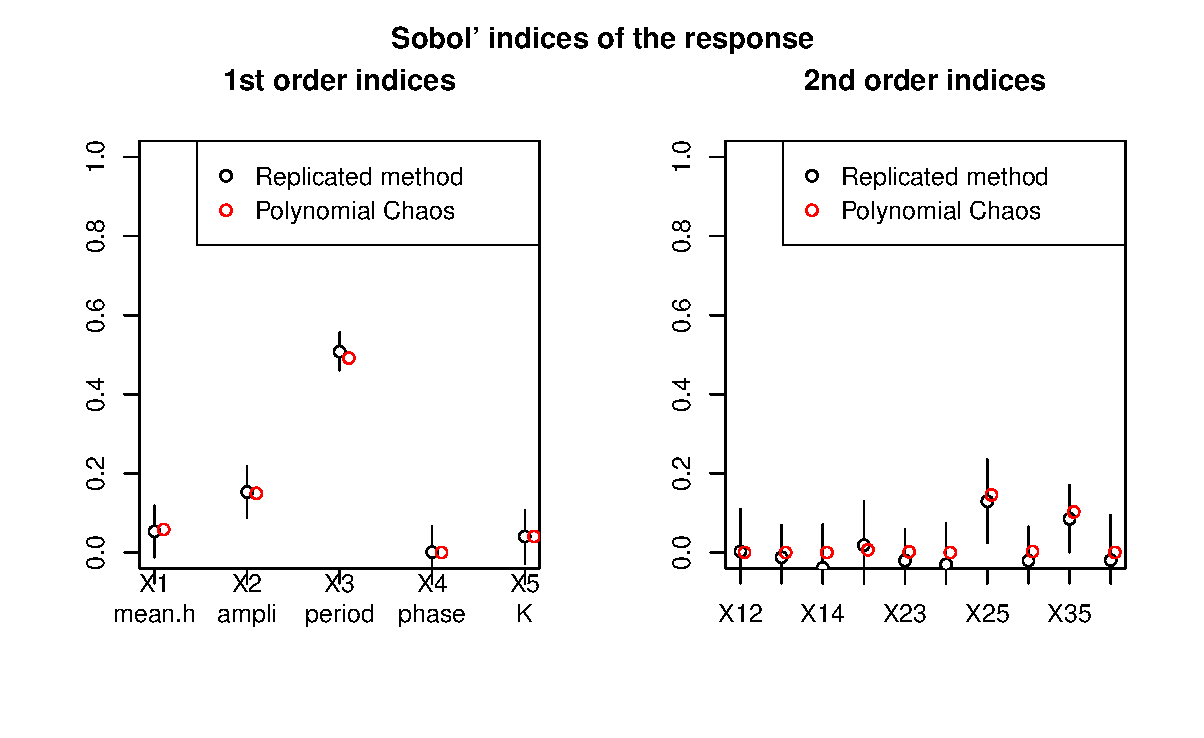
\includegraphics[width = \textwidth, height = .92\textheight]{sobol_J_PCE}
}
\frame{
\frametitle{Sobol' indices of the gradient of cost function}
$\frac{\mathrm{d}j}{\mathrm{d}K}(\bm{X}_e,K)$
  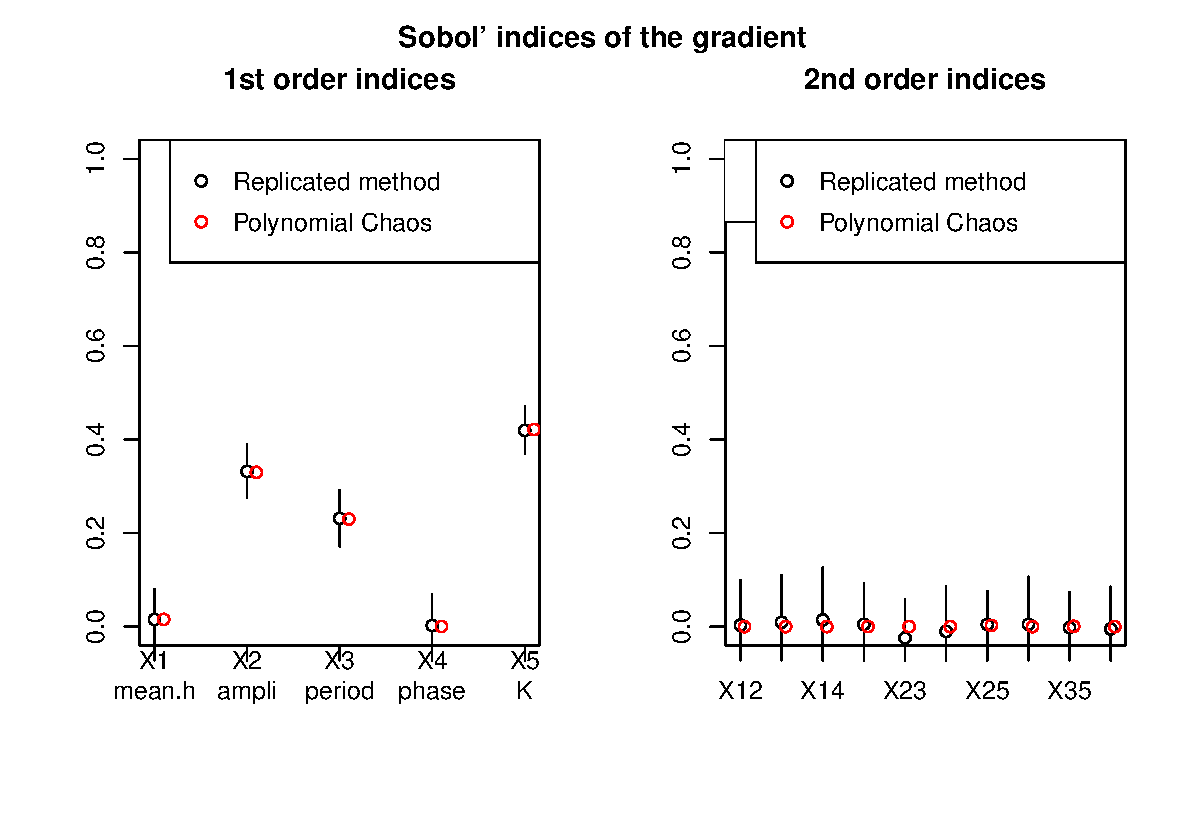
\includegraphics[width = \textwidth, height = .9\textheight]{sobol_G_PCE}
}
%\frame{
%$\argmin_K j(\bm{X}_e,K)$
%\frametitle{Sobol' indices of the output of the minimization procedure}
%  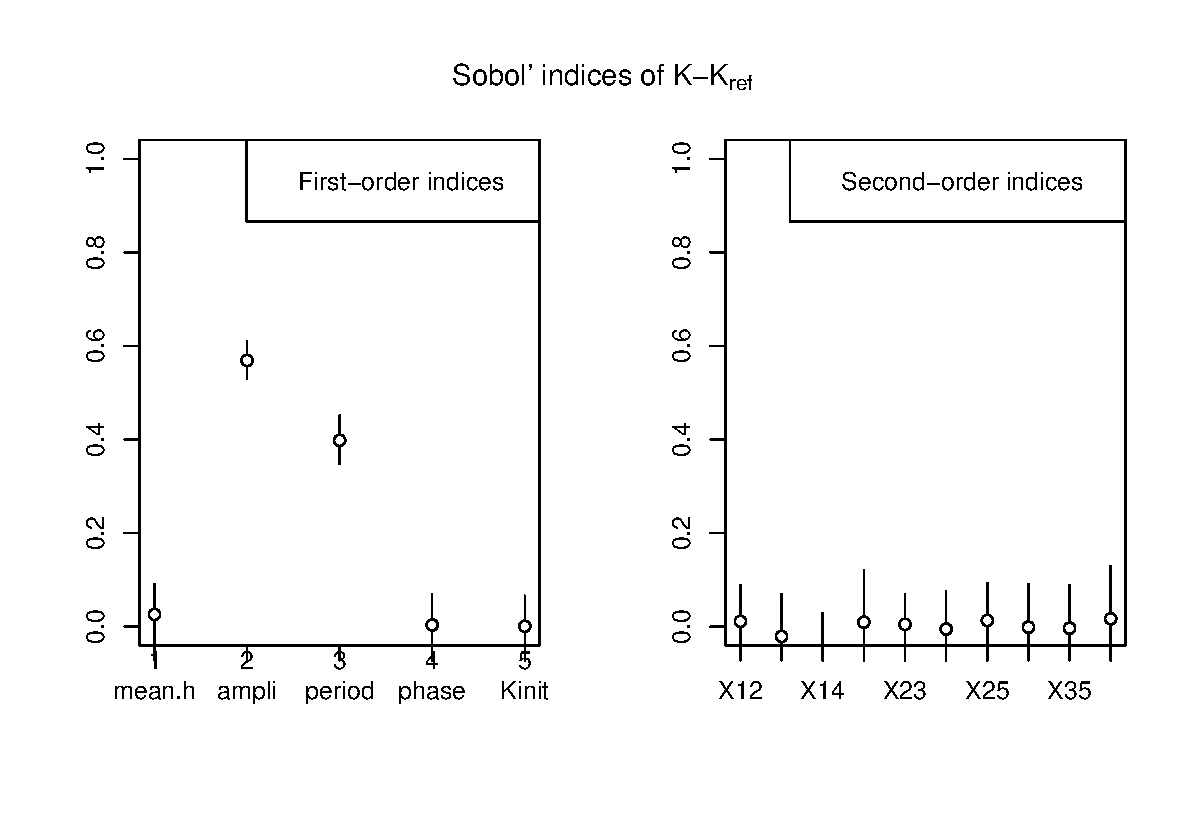
\includegraphics[width = \textwidth, height = .9\textheight]{sobol_Kargmin}
%}
\section{Robust Optimization}
\frame{
\frametitle{Robust Optimization}
\tableofcontents[
    currentsubsection, 
    sectionstyle=show/shaded, 
    subsectionstyle=show/hide,
    hideothersubsections
    ]
}

\frame{
	\frametitle{A first example}
	$(x_e,K) \mapsto f(x_e,K) = \tilde{f}(x_e+K)$ and $X_e \sim \mathcal{N}(0,s^2)$ truncated on $[{-3};3]$
	\begin{figure}[!h]
	\centering
	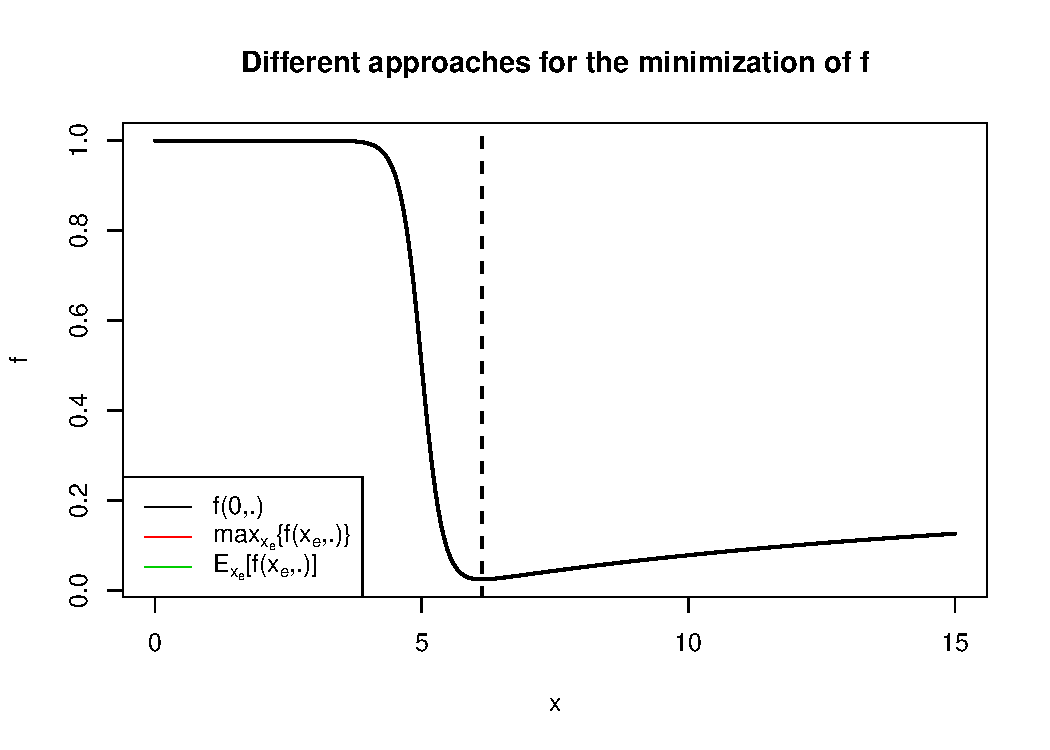
\includegraphics[scale = 0.6]{../Figures/mean_worstcase_robustness1}
	\end{figure}
}
\frame{
	\frametitle{A first example}
	$(x_e,K) \mapsto f(x_e,K) = \tilde{f}(x_e+K)$ and $X_e \sim \mathcal{N}(0,s^2)$ truncated on $[{-3};3]$
	\begin{figure}[!h]
	\centering
	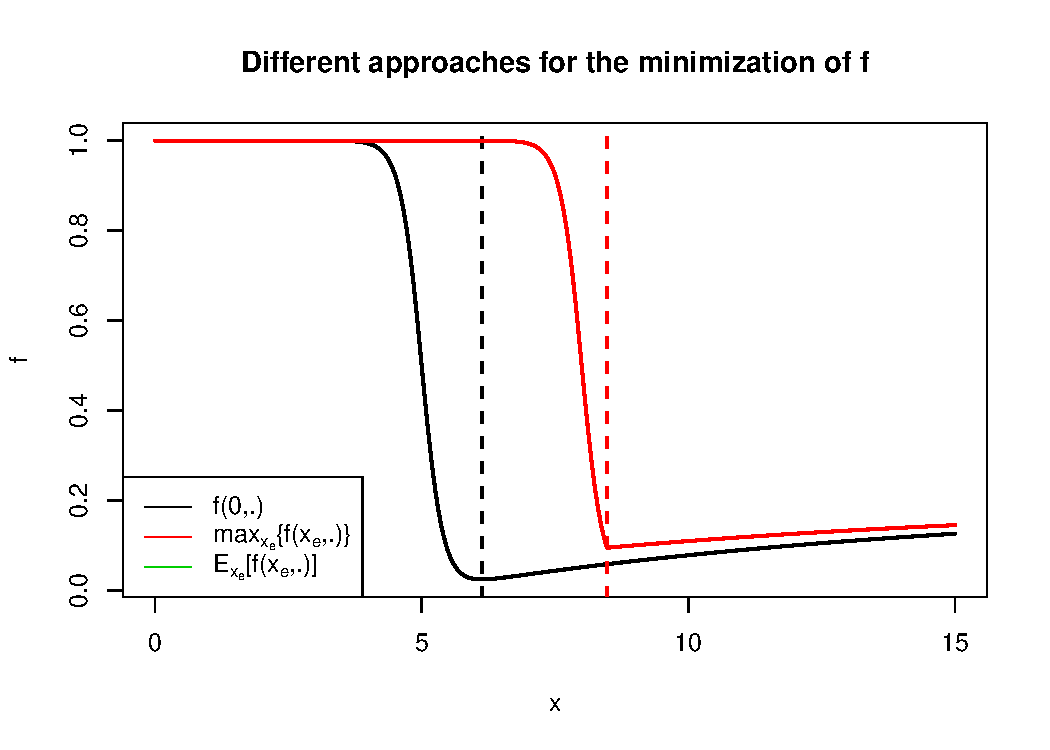
\includegraphics[scale = 0.6]{../Figures/mean_worstcase_robustness2}
	\end{figure}
}
\frame{
	\frametitle{A first example}
	$(x_e,K) \mapsto f(x_e,K) = \tilde{f}(x_e+K)$ and $X_e \sim \mathcal{N}(0,s^2)$ truncated on $[{-3};3]$
	\begin{figure}[!h]
	\centering
	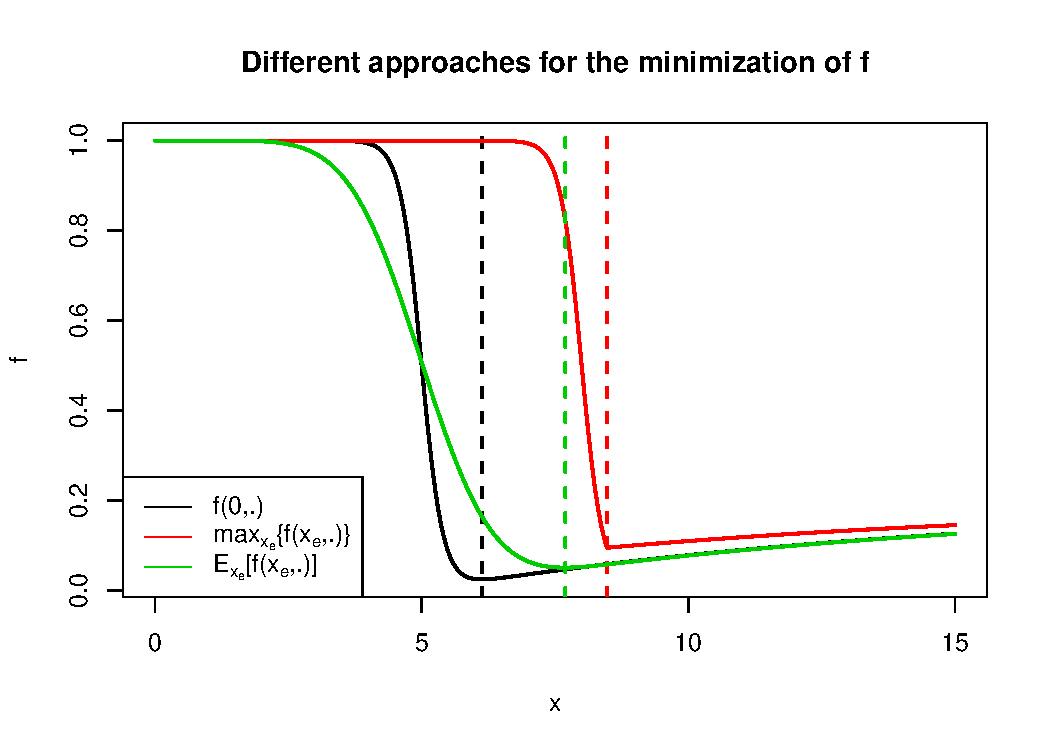
\includegraphics[scale = 0.6]{../Figures/mean_worstcase_robustness3}
	\end{figure}
}
\subsection{Concepts of robustness}
\frame{
\frametitle{Different Notions of robustness}
\begin{itemize}
\item<1-> Global Optimum: $ \min j(\bm{x}_e,K)$ $ \longrightarrow $ \alert<7->{EGO}
\item<2-> Worst case: $ \min_K \max_{\bm{x}_e} j(\bm{x}_e,K)$ $ \longrightarrow $ \alert<7->{Explorative EGO}
\item<3-> M-robustness: $\min \mu(K),\quad \text{constraint on } \sigma^2(K)$ $ \longrightarrow $ \alert<7->{iterated LHS}
\item<4-> V-robustness: $\min \sigma^2(K),\quad\text{constraint on } \mu(K)$ $ \longrightarrow $ gradient-descent with PCE
\item<5-> $\rho$-robustness: $\min \rho(\mu(K),\sigma^2(K))$ $\longrightarrow$ gradient-descent with PCE
\item<6-> Multiobjective: choice within Pareto frontier $\longrightarrow$ 1L/2L kriging
\end{itemize}
}
\subsection{Metamodeling}
\frame{
\frametitle{Why surrogates ?}
\begin{itemize}
\item Model $\longrightarrow$ expensive to run
\item High dimensional problem + taking into account uncertainties ?
\end{itemize}

\begin{center}
\only<1>{
\tikzstyle{block} = [rectangle, draw, fill=blue!20, 
     text centered, minimum width=1cm]
\tikzstyle{block2} = [rectangle, draw, fill=green!20, 
     text centered, , minimum width=6cm]

\tikzstyle{LHS}=[rectangle, draw, text centered]

\begin{tikzpicture}[node distance=3cm]

\node [align = center] at (0,0) (input) {Control variable \\$K \in \mathcal{K}$};
\node [align = center] at (4,1.5) (envir) {Environmental variables \\$\bm{X}_e$ random};
\node[block] at (4,0)(code){Direct Simulation};
\node[align = center] at (7,0) (output) {$W(\bm{x}_e,K)$};
\node[align = center] at (9.2,0) (jfun) {$j(\bm{x}_e,K)$};
\draw[->] (input) -- (code);
\draw[->] (envir) -- (code);
\draw[->] (code) -- (output);
\draw[->] (output) --(jfun);



\end{tikzpicture}}
\only<2>{
\tikzstyle{block} = [rectangle, draw, fill=blue!20, 
     text centered, minimum width=1cm]
\tikzstyle{block2} = [rectangle, draw, fill=green!20, 
     text centered, , minimum width=6cm]

\tikzstyle{LHS}=[rectangle, draw, text centered]

\begin{tikzpicture}[node distance=3cm]

\node [align = center] at (0,0) (input) {Control variable \\$K \in \mathcal{K}$};
\node [align = center] at (4,1.5) (envir) {Environmental variables \\$\bm{X}_e$ random};
\node[block] at (4,0)(code){Computer Code};
\node[align = center] at (7,0) (output) {$W(\bm{x}_e,K)$};
\node[align = center] at (9.2,0) (jfun) {$\bar{j}(\bm{x}_e,K)$};
\draw[->] (input) -- (code);
\draw[->] (envir) -- (code);
\draw[->] (code) -- (output);
\draw[->] (output) --(jfun);
\node[block2] at (5,0) (surr) {Metamodel};
\draw[->] (input) -- (surr);


\end{tikzpicture}}
\end{center}
%\includegraphics[width = 0.6\textwidth]{../Figures/Krig_EI_exampleBIG_cropped.pdf}
}
\frame{
\frametitle{Comparison between PCE and Kriging}
\begin{tabular}{l|c|c|}
 			& Polynomial Chaos & \alert<2>{Kriging} \\ \hline
Surrogate &  $J(\bm{X}) = \sum_{\bm{\alpha} \in \mathcal{A}} \hat{J}_{\bm{\alpha}}\bm{\Phi}_{\bm{\alpha}}(\bm{X})$ & $\bar{J}(\bm{x}) \sim \mathcal{N}(\hat{m}(\bm{x}),\hat{s}^2(\bm{x}))$ \\
Estim. & Numerical quadrature/Regression & Regression \\
Quantity & Statistical moments & estimate + CI  \\
Ref. & \cite{WienerChaos,sudretPCE2015} & \cite{krige1951,matheronUK} \\ \hline
\end{tabular}
}
\subsection{Adaptative sampling}
\frame{
\frametitle{Principle of adaptative sampling}
Based on kriging model $\longrightarrow$ mean and variance \\
How to choose a new point to evaluate ? 
Criterion $\kappa(\bm{x}) \longrightarrow$ "potential" of the point
\begin{equation*}
\bm{x}_{\mathrm{new}} = \argmax \kappa(\bm{x})
\end{equation*}
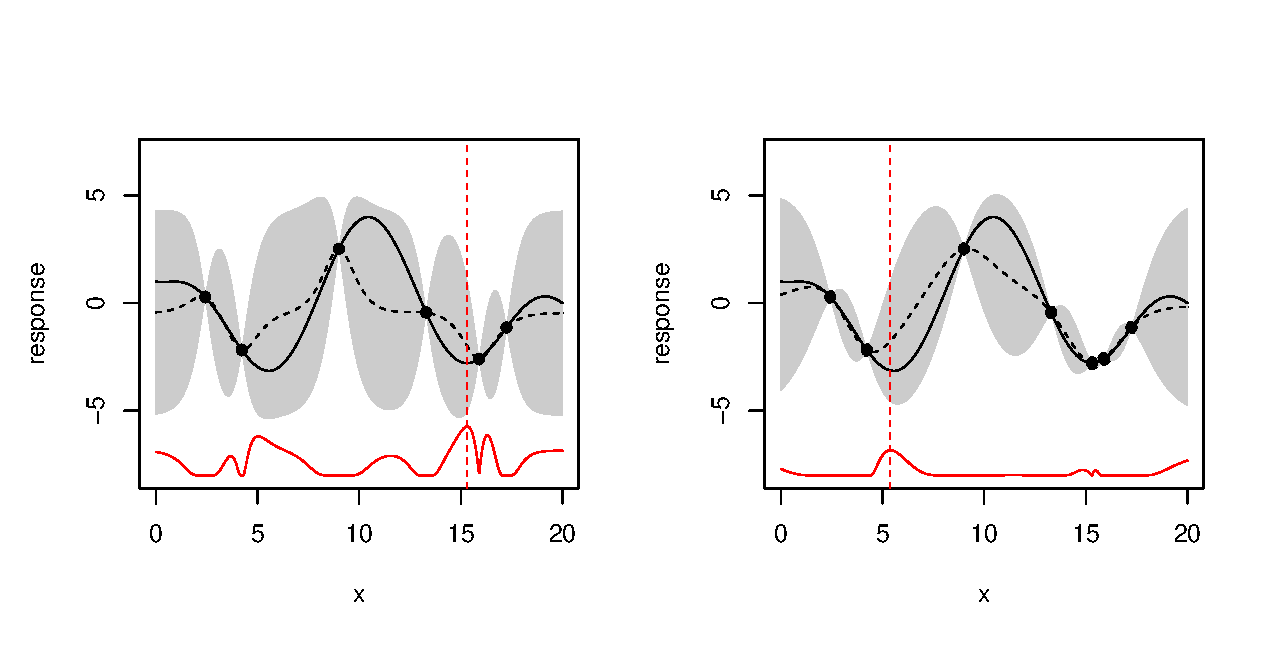
\includegraphics[width = \textwidth]{example_EGO}

}
\frame{
\frametitle{EGO \cite{Jones1998} \\ \emph{Global Optimum}}
$\mathcal{P}_N$ experimental design on $\mathbb{X} \times \mathcal{K}$, $\mathcal{Y}_N = j(\mathcal{P}_N)$.
\begin{equation*}
  \bar{J}_N(\bm{x}_e,K) \sim \mathcal{N}\left(\hat{m}_N(\bm{x}_e,K),\hat{s}_N^2(\bm{x}_e,K)\right)
\end{equation*}
%\only<1>{ \begin{figure}[!h]\centering 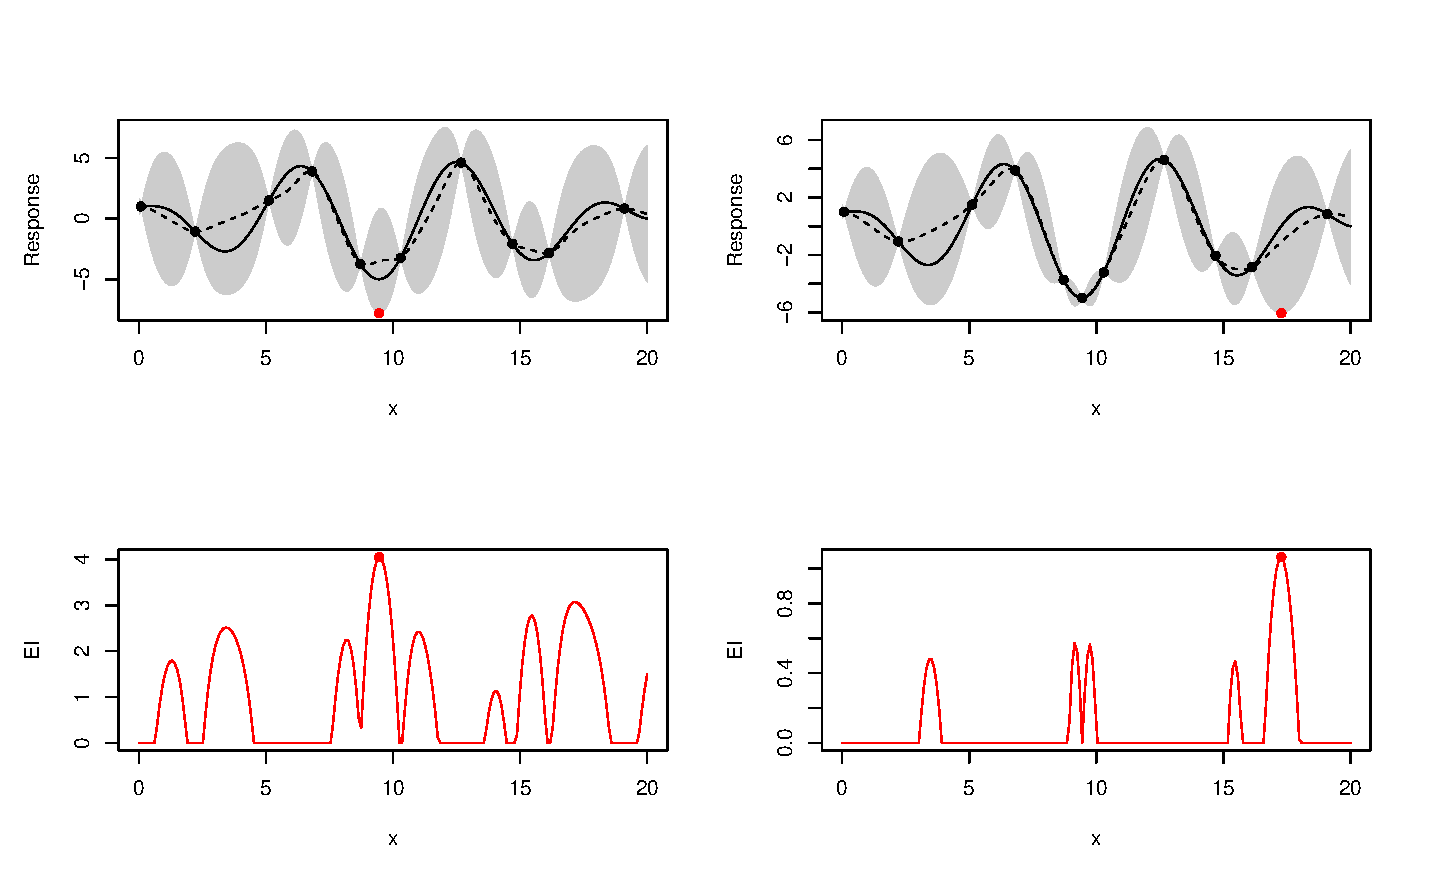
\includegraphics[width = \textwidth , trim = 0 7.5cm 12cm 0, clip]{Krig_EI_example} \end{figure}}
\onslide<2->{
$j_{\min}^N = \min \mathcal{Y}_N$ 
\begin{block}{Expected improvement}
\begin{align*}
 \only<4->{ EI(\bm{x}_e,K) = \Ex[}\only<3->{\max\{0, }j_{\min}^N - \bar{J}_N(\bm{x}_e,K) \only<3->{ \} } \only<4->{]} \\
  \end{align*}
\end{block}}
\onslide<5->{
\begin{block}{EGO iteration}
\begin{align*}
  (\tilde{\bm{x}}_e, \tilde{K}) = \argmax EI(\bm{x}_e,K)  \\
  \mathcal{P}_{N+1} = \mathcal{P}_N \cup (\tilde{\bm{x}}_e, \tilde{K}) \\
  \bar{J}_{N+1}(\bm{x}_e,K) \sim \mathcal{N}\left(\hat{m}_{N+1}(\bm{x}_e,K),\hat{s}_{N+1}^2(\bm{x}_e,K)\right)
\end{align*}
\end{block}}
}
\frame{
\frametitle{Example of an EGO iteration}
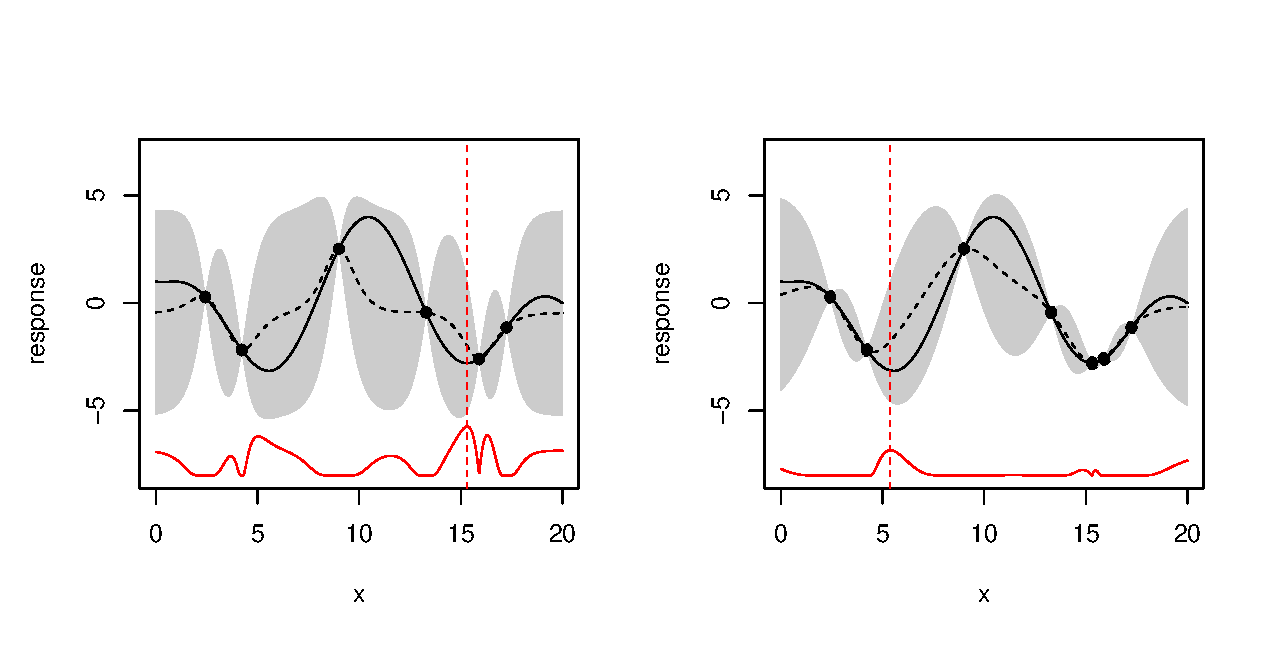
\includegraphics[width = \textwidth]{example_EGO}
}
\frame{
\frametitle{EGO}
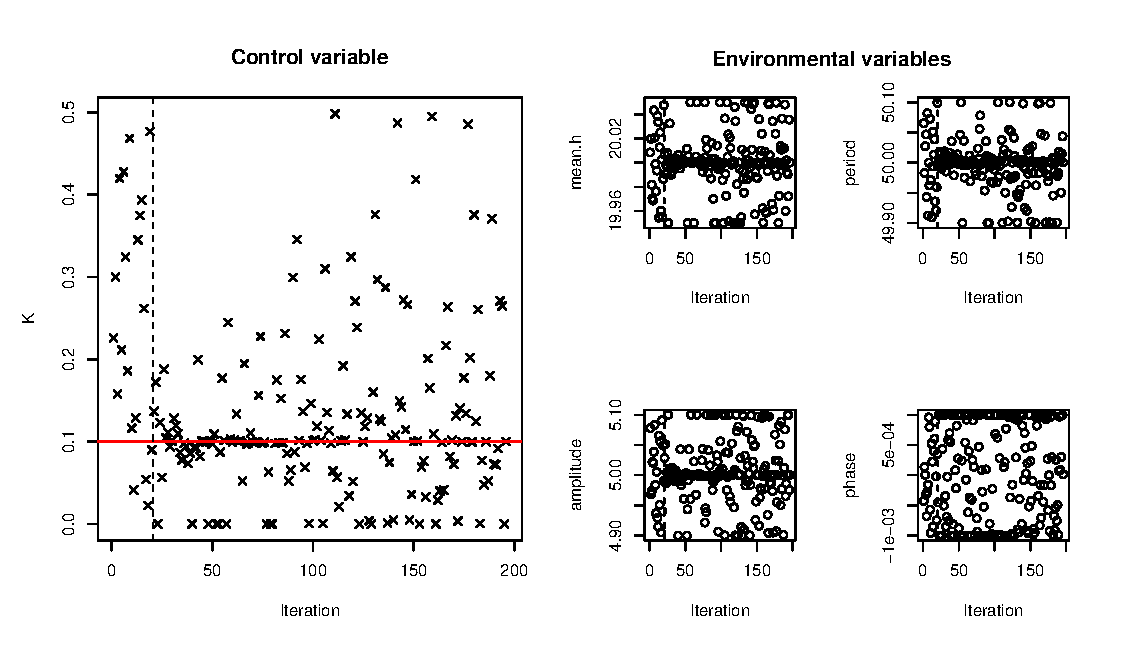
\includegraphics[width=\textwidth]{EGO_response}
%\begin{tabular}{|c|c|c|c|c|c|}
%EGO output & mean.h & amplitude & period & phase & $K$ \\ 
%  \hline
%$(\bm{x}_e,K)$ & 20.000083 & 5.000129 & 50.000309 & 0.000014 & 0.099971 \\ 
%\end{tabular}
}
\frame{
\frametitle{Explorative EGO  \cite{DesignCompExp}\\ \emph{Worst-case scenario}}
$\mathcal{P}_N$ experimental design on $\mathbb{X} \times \mathcal{K}$, $\mathcal{Y}_N = j(\mathcal{P}_N)$.
\begin{equation*}
  \bar{J}_N(\bm{x}_e,K) \sim \mathcal{N}\left(\hat{m}_N(\bm{x}_e,K),\hat{s}_N^2(\bm{x}_e,K)\right)
\end{equation*}
$j_{\min}^N = \min \mathcal{Y}_N$ 
\begin{block}{Expected improvement}
\begin{align*}
  EI(\bm{x}_e,K) = \Ex[\max\{0, j_{\min}^N - \bar{J}_N(\bm{x}_e,K) \} ]
\end{align*}
\end{block}\pause

\begin{block}{Explorative EGO iteration}
\begin{align*}
  (\tilde{\bm{x}}_e, \tilde{K}) = \argmax EI(\bm{x}_e,K)  \\
  \alert<3->{\bm{x}_e^* = \argmax_{\bm{x}_e} d\left((\bm{x}_e,\tilde{K}),\mathcal{P}_N \right)} \\
  \mathcal{P}_{N+1} = \mathcal{P}_N \cup (\bm{x}^*_e, \tilde{K}) \\
    \bar{J}_{N+1}(\bm{x}_e,K) \sim \mathcal{N}\left(\hat{m}_{N+1}(\bm{x}_e,K),\hat{s}_{N+1}^2(\bm{x}_e,K)\right)
\end{align*}
\end{block}
}
\frame{
\frametitle{Explorative EGO iterations \cite{DesignCompExp}}
\begin{figure}
\centering
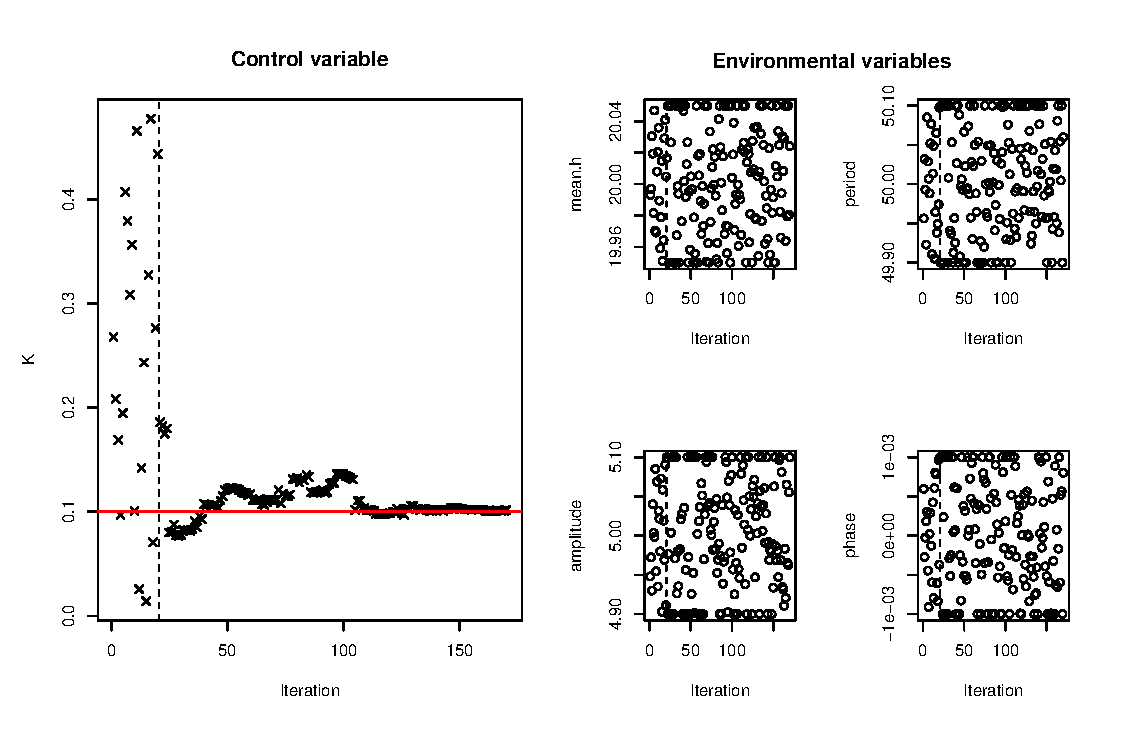
\includegraphics[width=\textwidth]{exploEGO}
\end{figure}
}

\frame{
\frametitle{Iterated LHS\\\emph{M-robustness}}
\begin{center}
\scalebox{.7}{\tikzstyle{block} = [rectangle, draw, fill=blue!20, 
     text centered, rounded corners, minimum width=1cm]

\tikzstyle{block2} = [rectangle, draw, fill=green!20, 
     text centered, rounded corners, minimum width=1cm]

\tikzstyle{LHS}=[rectangle, draw, text centered]

\begin{tikzpicture}[node distance=3cm]

\draw [->] (-1,0) -- (4.5,0) node [above,very near end] {$K$};

\draw[-] (-0.75,0.1) -- (-0.75,-0.1) {};
\draw[-] (0.2,0.1) -- (0.2,-0.1) node [midway] {};
%\draw[-] (-1,0.1) --(-1,-0.1) node [midway] {};
\draw[-] (4,0.1) --(4,-0.1) node [midway] {};
\draw[->] (-0.75,0) -- (-0.75,-1) node[midway] {};
\draw[->] (0.2,0) -- (.95,-1) node[midway] {};
\draw[->] (4,0) -- (4,-1) node[midway] {};

\draw [fill=blue!20, align = center] (-1.5,-1) rectangle (0,-2.5) node[midway] (lhs1) {LHS \\ on $\mathbb{X}$};
\draw [fill=blue!20, align = center] (0.2,-1) rectangle (1.7,-2.5) node[midway] (lhs2) {LHS \\ on $\mathbb{X}$};
\draw [fill=blue!20, align = center] (3,-1) rectangle (4.5,-2.5) node[midway] (lhs3) {LHS \\ on $\mathbb{X}$};
\node (dots) at (2.35,-1.75)  {$\dots$};

\end{tikzpicture}
}
\end{center} to build $\hat{\mu}(K)$ and $\hat{\sigma}^2(K)$\pause
\begin{block}{Estimate of the mean}
\begin{gather*}
\Ex[J(\bm{X}_e,K) | K] \xrightarrow{\mathrm{estimator}} {\hat{\mu}}(K) = n_e^{-1}\sum_{i=1}^{n_e}J(\bm{X}^{i}_e,K) \text{ (r.v.)} \\
\Var[J(\bm{X}_e,K) | K] \xrightarrow{\mathrm{estimator}} {\hat{\sigma}}^ 2(K) = (n_e-1)^{-1}\sum_{i=1}^{n_e} (J(\bm{X}^{i}_e,K) - \hat{\mu}(K))^2 \text{ (r.v.)}  \\ 
\Ex[\hat{\mu}(K)] = \Ex[J(\bm{X}_e,K) | K] \quad\text{ and} \quad \Var[\hat{\mu}(K)] = \frac{\Var[J(\bm{X}_e,K) | K]}{n_e} \approx \frac{\hat{\sigma}^ 2(K)}{n_e}
\end{gather*}
\end{block}
}
\frame{
\begin{block}{Estimated mean as a random variable}
\begin{equation}
	\hat{\mu}(K) \sim \mathcal{N}\left(\Ex[J(\bm{X}_e,K) | K], \frac{\hat{\sigma}^ 2(K)}{n_e}\right) \tag{CLT approximation}
\end{equation}

\end{block}
Idea \cite{rulliere} :
\begin{itemize}
\item Add a new point $K_{\mathrm{new}}$ and estimate $\Ex[J(\bm{X}_e,K) | K = K_{\mathrm{new}}]$
\item OR Reduce the variance by increasing $n_e$
\end{itemize}
\pause
In an adaptative sampling strategy: $K^* = \argmax_{K\in \mathcal{K}} \kappa(K)$
\begin{itemize}
\item if $K^*$ "close" to an existing point $\longrightarrow$ increase $n_e$
\item if not $\longrightarrow$ add $K^*$ to the design
\end{itemize}
}
\frame{
\frametitle{Knowledge-gradient criterion}
Metamodel of the \emph{estimated} mean: \\
Based on $\mathcal{P}_N$, an experimental design of $N$ points on $\mathcal{K}$.
\begin{equation*}
	\bar{\mu}_N(K) \sim \mathcal{N}\left(\hat{m}_N(K),\hat{s}_N^2(K)\right)
\end{equation*}
\pause
In the presence of noise in the kriging model:
\begin{block}{Definition of the KG \cite{frazier2008seq}}
\begin{equation*}
  KG(\tilde{K}) = \min_{K'\in\mathcal{K}} \hat{m}_N(K') - \Ex\left[ \min_{K'\in\mathcal{K}} \hat{m}_{N+1}(K') \middle|\, \tilde{K} \right]
\end{equation*}
\end{block}
where $\hat{m}_{N+1}$ is the kriging mean computed based on $\mathcal{P}_N \cup \{\tilde{K} \}$
\begin{center}
\scalebox{0.66}{\tikzstyle{block} = [rectangle, draw, fill=blue!20, 
     text centered, rounded corners, minimum width=1cm]

\begin{tikzpicture}[node distance=3cm]
% \draw [fill=red!10] (4.8,2.2) rectangle (10.3,-2.2) node[midway] {\emph{Kriging Layer}};
\node [block] (jfun)  {$j$};
% \node [block, right of =jfun] (jfuneval2) {$j(\mathcal{P}_{K_2})$};
% \node [block, above of = jfuneval2] (jfuneval1) {$j(\mathcal{P}_{K_1})$};
% \node [block,below of = jfuneval2] (jfuneval3) {$j(\mathcal{P}_{K_3})$};
\node[block, right of = jfun] (jfuneval) {$\{j(\mathcal{P}_{K_i})\}_{1 \leq i \leq N}$};
\node [right of = jfuneval] (void1) {};
\node [right of = void1] (void2) {};
\node[block] at (6.5,1.5) (muhat){$\{\hat{\mu}(K_i)\}_{1\leq i \leq N}$};
\node[block] (sigmahat) at (6.5,-1.5) {$\{\hat{\sigma}^2(K_i)\}_{1\leq i \leq N}$};
\node[block, right of = void1](mu1L) {$\bar{\mu}_N(K)$};
\node[block, right of = mu1L] (KG) {$K_{N+1}$};
\node[above of = mu1L] (abmu) {};
\node[below of= mu1L]  (bemu) {};
% \node[block, right of = sigmahat](sigma1L) {$\bar{\sigma}^2(K)$};
% \node[block, right of = void2](pareto) {Pareto front};
\draw [->] (jfun) -- (jfuneval) node [above,midway] {LHS};
\draw [->] (jfuneval) -- (muhat);
\draw [->] (jfuneval) -- (sigmahat);
\draw [->] (muhat) -- (mu1L);b
\draw[->](sigmahat) -- (mu1L);

\draw[->] (mu1L) -- (KG) node [above, midway] {$KG$};
\node[block, align = left] (newpoints) at (3,2) {$K_{N+1}$ added\\$N \gets N+1$};
\node[block] (adding) at (3,-2) {$\mathcal{P}_{K_i}$ augmented};
\draw[->] (KG) --(12,2) node[near end, left, align=right] {above \\threshold}-- (newpoints);
\draw[->] (newpoints) -- (jfuneval);
\draw[->] (KG) --(12,-2) node[near end, left, align=right] {below \\threshold} -- (adding);
\draw[->] (adding) -- (jfuneval);
\node (krig) at (7.8,0) {Krig.};
% \draw [->] (sigmahat) -- (sigma1L) node [above,midway] {Krig.};
% \draw [->] (sigma1L) -- (pareto);
% \draw [->] (mu1L) -- (pareto);

\end{tikzpicture}

}
\end{center}
}



\frame{
\frametitle{Iterated LHS}
\includegraphics<1>[width = \textwidth]{thres005_1}
\includegraphics<2>[width = \textwidth]{thres005_2}
\includegraphics<3>[width = \textwidth]{thres005_3}
\includegraphics<4>[width = \textwidth]{thres005_4}
\includegraphics<5>[width = \textwidth]{thres005_5}
\includegraphics<6>[width = \textwidth]{thres005_6}
%\includegraphics<7>[width = \textwidth]{Figures/thres005_7}
%\includegraphics<8>[width = \textwidth]{Figures/thres005_8}
%\includegraphics<9>[width = \textwidth]{Figures/thres005_9}
%\includegraphics<10>[width = \textwidth]{Figures/thres005_10}
}

\section{Conclusion}

\frame{
	\frametitle{Wrapping up}
	\begin{itemize}
	\item Notion of robustness
	\item Metamodelling techniques $\rightarrow$ include uncertainties
	\item Balance between precision and number of runs
	\end{itemize}
}

\frame{
	\frametitle{Perspective and future work}
	\begin{itemize}
	\item Better numerical model
	\begin{itemize}
		\item 2D
		\item Better numerical scheme
	\end{itemize}
	\item Influence of observation operator $\mathcal{H}$
	\begin{itemize}
		\item $Y$ as real measurements
	\end{itemize}
	\item Extension to $K$ multidimensional 
	\item Choice of metamodel:
		\begin{itemize}
		\item Kriging
		\begin{itemize}
			\item not adapted to high-dimensional input space
			\item Adaptative sampling in multidimensional case? 
		\end{itemize}
		\item PC
			\begin{itemize}
			\item adapted to $K$ multidimensional
			\item "Fixed" grid to evaluate
			\item May need more evaluation in some cases + adjoint
			\end{itemize}
		\end{itemize}
	\end{itemize}

}

\frame{
	\frametitle{Thank you for your attention}
	\begin{multicols}{2}
	\tableofcontents
	\end{multicols}
}

\begin{frame}[allowframebreaks]
\bibliographystyle{apalike}
\bibliography{biblio.bib}
\end{frame}
\section*{Appendix}
\subsection*{The Adjoint Model}

\frame{
\frametitle{Principle of the adjoint method}
Let us assume that we have the (formal) model
\begin{align}
 & J(W(K),K) \tag{Cost function} \\
\text{s.t.}&\,R(W(K),K) = 0 \tag{Model equation (SWE)}
\end{align}
\begin{overprint}
\onslide<2->{\begin{equation}
\frac{\mathrm{d}J}{\mathrm{d}K} = ?
\end{equation}}
\onslide<3->{
\begin{align}
\frac{\mathrm{d}J}{\mathrm{d}K} &= \frac{\partial J}{\partial W} \textcolor{red}{\frac{\partial W}{\partial K}} +\frac{\partial J}{\partial K} \\
\frac{\mathrm{d}R}{\mathrm{d}K} &= \frac{\partial R}{\partial W} \textcolor{red}{\frac{\partial W}{\partial K}} +\frac{\partial R}{\partial K} =0
\end{align}
}
\end{overprint}
\onslide<4->{
And by introducing a Lagrange multiplier $\lambda$
}
}
\frame{
\frametitle{Principle of the adjoint method}
\begin{align}
\frac{\mathrm{d}J}{\mathrm{d}K} &= \frac{\partial J}{\partial W} \frac{\partial W}{\partial K} +\frac{\partial J}{\partial K} - \lambda^T \left(\frac{\partial R}{\partial W} \frac{\partial W}{\partial K} +\frac{\partial R}{\partial K}\right)\\
&= \underbrace{\left(\frac{\partial J}{\partial W} - \lambda^T\frac{\partial R}{\partial W} \right)}_{=0 \text{ if } \lambda \text{ is choosen wisely}}\frac{\partial W}{\partial K} + \left(\frac{\partial J}{\partial K} - \lambda^T\frac{\partial R}{\partial K}\right) 
\end{align}
\begin{block}{Adjoint model}
	\begin{equation}
		\left(\frac{\partial R}{\partial W} \right)^T \lambda = 	\left( \frac{\partial J}{\partial W}\right)^T
	\end{equation}
\end{block}
\pause
For a value $K$:
\begin{itemize}
\item<3-> solve $R(W(K),K) = 0$ for $W$
\item<4-> solve $ \left(\frac{\partial R}{\partial W} \right)^T \lambda = 	\left( \frac{\partial J}{\partial W}\right)^T$ for $\lambda$
\item<5-> compute $\frac{\mathrm{d}J}{\mathrm{d}K}$
\end{itemize}
}

\subsection*{Polynomial Chaos}
\frame{
\frametitle{Orthogonal Polynomials in a Hilbert space}
$X$, $J(X)$ r.v., such that $\Ex[X^2],\Ex[J(X)^2] < +\infty$\\
$\rightarrow$ Expand $J$ on a basis of orthogonal polynomials with respect to a specific inner product \cite{WienerChaos,sudretPCE2015}. \pause\\
Functional inner product:

\begin{align*}
\langle f, g \rangle = \int_{D_X} f(\xi)g(\xi)p_X(\xi) \, \mathrm{d}\xi
\end{align*}

\begin{block}{Family of orthogonal polynomials}
\begin{equation*}
	\langle \varphi_i , \varphi_j \rangle = \|\varphi_i \|^2 \delta_{ij}
\end{equation*}
\end{block}

\begin{table}
\scalebox{.8}{
	\begin{tabular}{|c|c|c|c|} \hline
		Family & $D_X$ & p.d.f. & Distribution \\ \hline
		Legendre & $[-1;1]$ & $p_X(\xi) = {}^1\!/\!_2$ & $\mathcal{U}([-1;1])$\\ 	\hline 
		Hermite & $\mathbb{R}$ & $p_X(\xi) = e^{-\xi^2/2}$ & $\mathcal{N}(0,1)$ \\ \hline
		Laguerre & $[0,+\infty[$ & $p_X(\xi) = e^{-\xi}$ & $\mathrm{Exp}$ \\ \hline
	\end{tabular} }
\end{table}


}
\frame{
\frametitle{The expansion as a surrogate model}
\begin{block}{Polynomial Chaos Expansion, 1D}
	\begin{equation*}
	\mathcal{J} = J(X) = \sum_{i=0}^{+\infty} \hat{J}_i \varphi_i(X) \approx \sum_{i=0}^P \hat{J}_i \varphi_i(X) 
	\end{equation*}
\end{block}
\pause
	\begin{align*}
		\bm{\alpha} &= (\alpha_1,\dots \alpha_p),\quad |\bm{\alpha}| = \sum_i \alpha_i \nonumber \\
	\Phi_{\bm{\alpha}}(\bm{X}) &= \prod_i \varphi_{\alpha_i}(X_i) \nonumber
	\end{align*}
\begin{block}{Polynomial Chaos Expansion, multidimensional}
	\begin{align*}
	\mathcal{J} = J(\bm{X}) &= \sum_{|\bm{\alpha}|=0}^{+\infty} \hat{J}_{\bm{\alpha}} \Phi_{\bm{\alpha}}(\bm{X}) \approx  \sum_{|\bm{\alpha}| \leq P} \hat{J}_{\bm{\alpha}} \Phi_{\bm{\alpha}}(\bm{X}) \\
	\end{align*}
\end{block}
}
\frame{
\frametitle{Statistical moments using PCE}
PCE allows us to get easily the statistical moments:
\begin{block}{Mean and variance of $\mathcal{J}$ using the coefficients of the expansion}
\begin{align*}
  \Ex[\mathcal{J}] &= \hat{J}_0\|\bm{\Phi}_0\|^2 = \hat{J}_0 \\ 
\Var[\mathcal{J}] = \Ex[\mathcal{J}^2] - \Ex[\mathcal{J}]^2 &= \sum_{|\bm{\alpha}|\leq P} \hat{J}^2_{\bm{\alpha}} \|\bm{\Phi}_{\bm{\alpha}}\|^2 - \hat{J}^2_0 = \sum_{0<|\bm{\alpha}|\leq P} \hat{J}^2_{\bm{\alpha}} \|\bm{\Phi}_{\bm{\alpha}}\|^2
\end{align*}
\end{block}
}
\frame{
\frametitle{PCE on the response}
\begin{center}
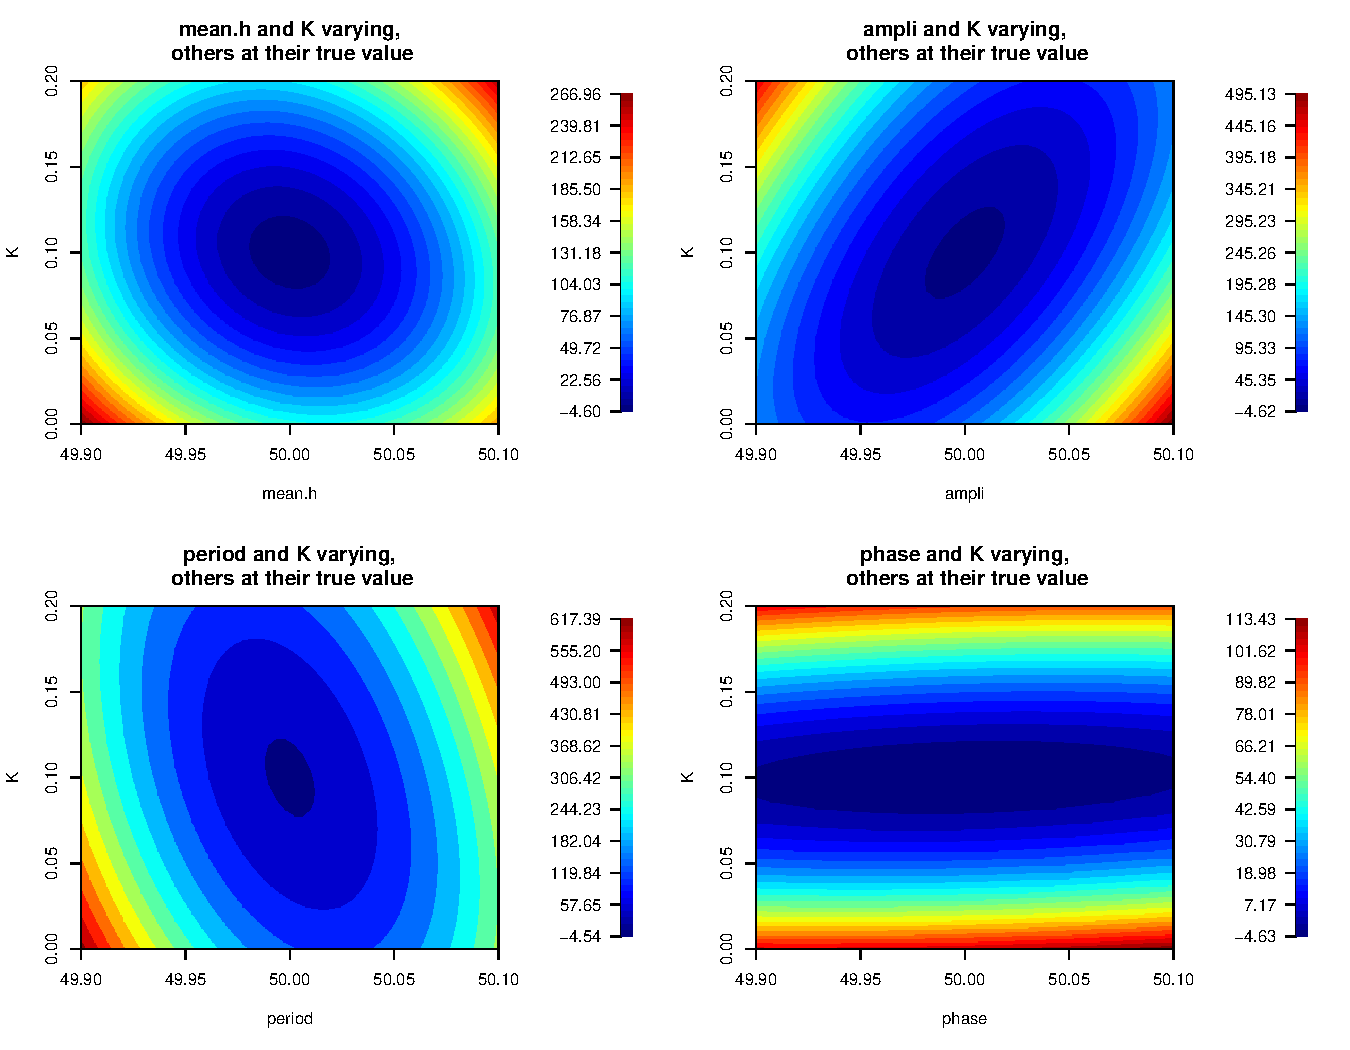
\includegraphics[width = .8\textwidth]{PCE_tot}
\end{center}
}

\subsection*{Kriging}
\frame{
	\frametitle{Principle of Kriging}
	$\mathcal{X} = \{\bm{x}^{(1)},\dots,\bm{x}^{(n_s)}\}$ and $\mathcal{Y} = j(\mathcal{X})$ \\
	We assume that the deterministic model $j(\bm{x})$ is the realization of a GP  \cite{krige1951, matheronUK}:
	\begin{block}{Kriging formalism}
	\begin{gather*}
	  \underbrace{J(\bm{x})}_{\text{r.v.}} = \underbrace{\bm{f}(\bm{x})^T\bm{\beta}}_{\text{deter}} + \underbrace{\varepsilon(\bm{x})}_{\text{r.v.}} \\
	  \Ex[\varepsilon(\bm{x})] = 0 \quad \text{ and } \quad\mathrm{Cov}(\varepsilon(\bm{x}),\varepsilon(\bm{x'})) = \sigma^2_J \underbrace{R(\bm{x},\bm{x'})}_{\text{Chosen}}\\
	  \bar{J}(\bm{x}) \sim J(\bm{x}) | \mathcal{Y}
	\end{gather*}
	\end{block}
}
\frame{
\frametitle{Kriging predicator}
{\small
\begin{align*}
  \bm{F} &= \{f_j(\bm{x}^{(i)}) \}_{\substack{1 \leq i \leq n_s \\ 1 \leq j \leq n_\beta}} \\
  \bm{R} &= \{R(\bm{x}^{(i)},\bm{x}^{(j)}) \}_{1 \leq i,j \leq n_s} \\
  \bm{r}(\bm{x}) &= \left[R(\bm{x}^{(1)},\bm{x}),\dots,R(\bm{x}^{(n_s)},\bm{x}) \right]^T
\end{align*}
\begin{block}{Joint distribution of $\mathcal{Y}$ and $J$}
\begin{equation*}
  \begin{bmatrix}
    \mathcal{Y} \\ J(\bm{x})
  \end{bmatrix} \sim \mathcal{N}\left(
    \begin{bmatrix}
      \bm{F} \hat{\bm{\beta}} \\
      \bm{f}(\bm{x})^T \hat{\bm{\beta}}
    \end{bmatrix}, \sigma_J^2
    \begin{bmatrix}
      \bm{R} & \bm{r}(\bm{x}) \\
      \bm{r}(\bm{x})^T & 1
    \end{bmatrix}
\right)
\end{equation*}
\end{block}
}
\begin{block}{Kriging predicator $\bar{J}$}
\begin{align*}
\bar{J}(\bm{x}) &\sim  J(\bm{x}) | \mathcal{Y} \\
			&\sim \alert<2>{\mathcal{N}(\hat{m}_J(\bm{x}) , \hat{s}^2_J(\bm{x}))}
\end{align*}
\end{block}
}
\frame{
\frametitle{Example of kriging}
\begin{figure}[!h]\centering 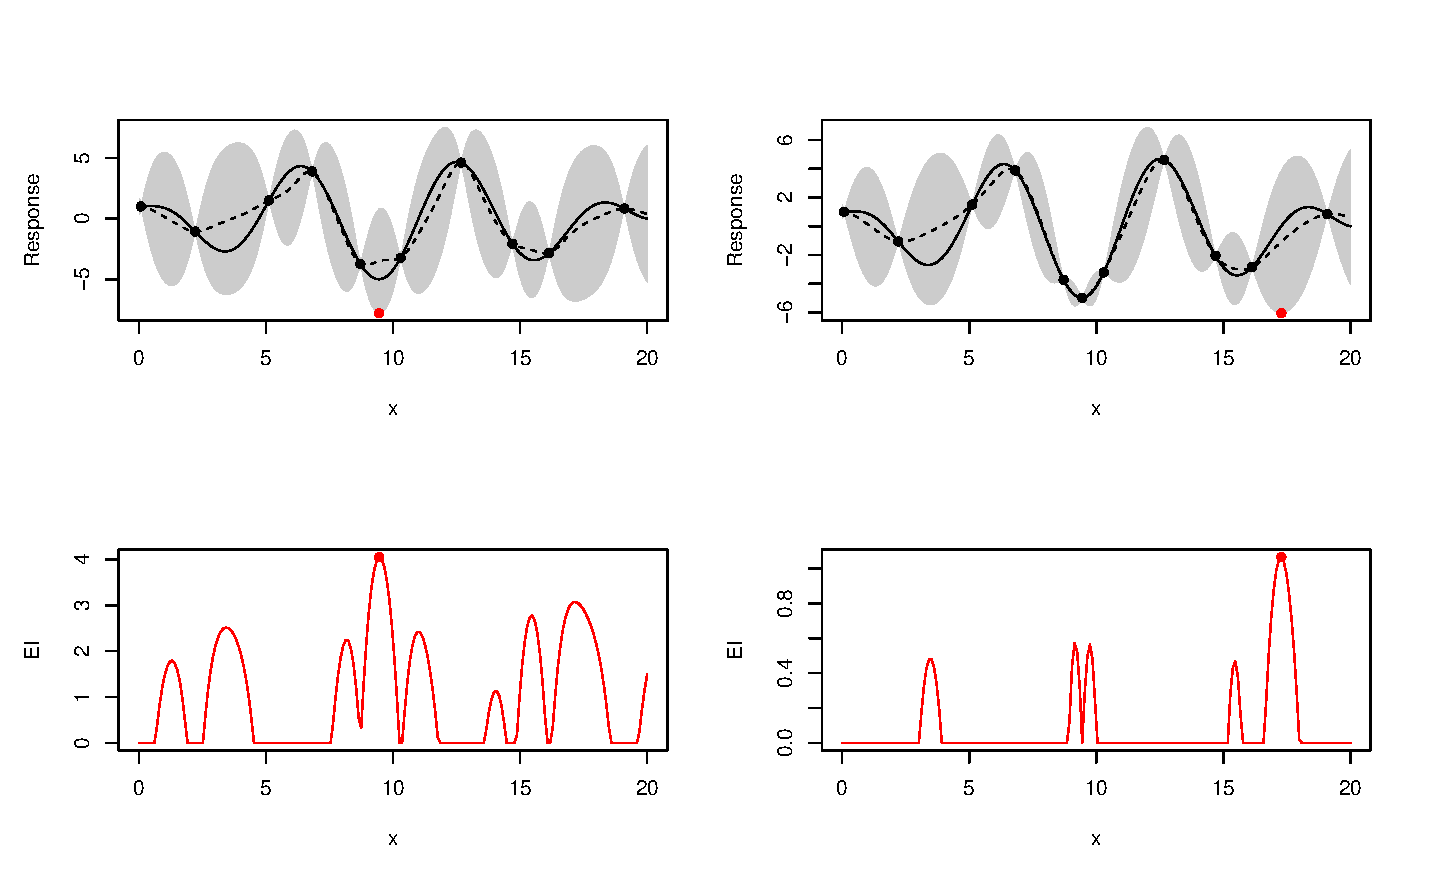
\includegraphics[width = \textwidth , trim = 0 7.5cm 12cm 0, clip]{Krig_EI_example} \end{figure}

}
\frame{
\frametitle{Example of kriging}
\begin{figure}[!htbp]
  \centering
  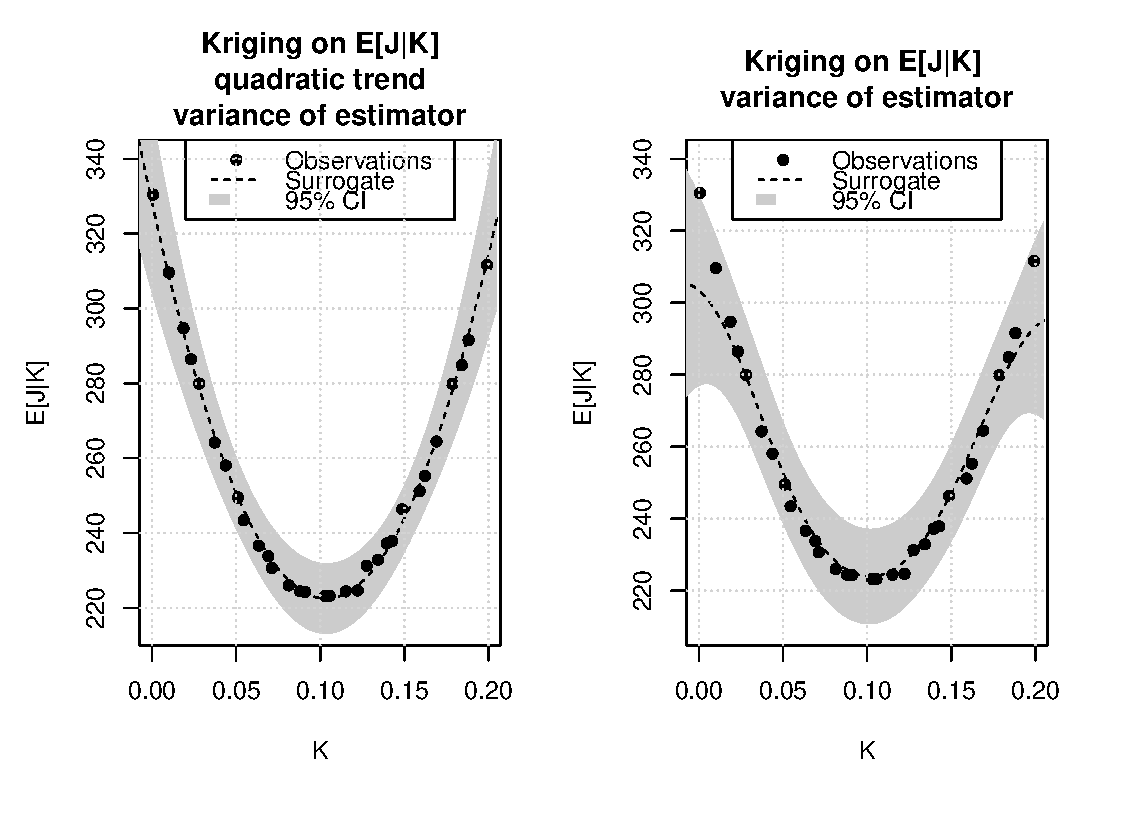
\includegraphics[width = 0.8\textwidth]{mu_krig_trend} 
  \caption{Kriging with and without trend of the estimate mean. Variance of observations based on the variance of the estimate}
  \label{fig:mu_trend}
\end{figure}
}
\subsection*{Exhaustive computation using surrogates}
\frame{
	\frametitle{Multi-objective problem: general vocabulary}
	Vector of objective functions $\bm{f} = (f_1,\dots,f_r)$:
	\begin{block}{Pareto domination relation}
	\begin{equation*}
		\bm{f}(\bm{x}) \prec \bm{f}(\bm{x}') \text{ if } \begin{cases}  f_j(\bm{x}) \leq f_j(\bm{x}') & \forall j \leq r \\
				f_j(\bm{x}) < f_j(\bm{x}') & \text{ for one } j \leq r
		\end{cases}
	\end{equation*}
	\end{block} \pause
	\begin{block}{Pareto set, front}
	Pareto set:
	\begin{equation*}
		\mathfrak{P} = \{ \bm{x} \text{ s.t. } \nexists \bm{x}', \bm{f}(\bm{x}') \prec \bm{f}(\bm{x}) \}
	\end{equation*}
	Pareto front:
	\begin{equation*}
			\{ \bm{z} \text{ s.t. } \exists \bm{x} \in \mathfrak{P}, \bm{z} = \bm{f}(\bm{x})\}
	\end{equation*}
	\end{block}
}

\frame{
 \frametitle{Kriging to estimate the Pareto front \\\cite{dellino2012robust}}
 	Minimization of the vector $(\mu(K),\sigma^2(K))$ \\
	Idea: Replace expensive computations of $(\mu(K),\sigma^2(K))$ by cheap computations of the metamodel \\
	
	\begin{itemize}
	\item<2->  Initial design on $\mathcal{K}$, compute for each one $\hat{\mu}$ and $\hat{\sigma}^2$, and generate a surrogate
	\item<3->  Initial design on $\mathbb{X} \times \mathcal{K}$, and use a surrogate to estimate mean and variance
	\end{itemize}
}
\frame{
	\frametitle{1L-Kriging}
\begin{center}
\scalebox{.6}{\tikzstyle{block} = [rectangle, draw, fill=blue!20, 
     text centered, rounded corners, minimum width=1cm]

\tikzstyle{block2} = [rectangle, draw, fill=green!20, 
     text centered, rounded corners, minimum width=1cm]

\tikzstyle{LHS}=[rectangle, draw, text centered]

\begin{tikzpicture}[node distance=3cm]

\draw [->] (-1,0) -- (4.5,0) node [above,very near end] {$K$};

\draw[-] (-0.75,0.1) -- (-0.75,-0.1) {};
\draw[-] (0.2,0.1) -- (0.2,-0.1) node [midway] {};
%\draw[-] (-1,0.1) --(-1,-0.1) node [midway] {};
\draw[-] (4,0.1) --(4,-0.1) node [midway] {};
\draw[->] (-0.75,0) -- (-0.75,-1) node[midway] {};
\draw[->] (0.2,0) -- (.95,-1) node[midway] {};
\draw[->] (4,0) -- (4,-1) node[midway] {};

\draw [fill=blue!20, align = center] (-1.5,-1) rectangle (0,-2.5) node[midway] (lhs1) {LHS \\ on $\mathbb{X}$};
\draw [fill=blue!20, align = center] (0.2,-1) rectangle (1.7,-2.5) node[midway] (lhs2) {LHS \\ on $\mathbb{X}$};
\draw [fill=blue!20, align = center] (3,-1) rectangle (4.5,-2.5) node[midway] (lhs3) {LHS \\ on $\mathbb{X}$};
\node (dots) at (2.35,-1.75)  {$\dots$};

\end{tikzpicture}
}
\end{center}
\scalebox{0.8}{\tikzstyle{block} = [rectangle, draw, fill=blue!20, 
     text centered, rounded corners, minimum width=1cm]

\begin{tikzpicture}[node distance=3cm]
\draw [fill=red!10] (4.8,2.2) rectangle (10.3,-2.2) node[midway] {\emph{Kriging Layer}};
\node [block] (jfun)  {$j$};
% \node [block, right of =jfun] (jfuneval2) {$j(\mathcal{P}_{K_2})$};
% \node [block, above of = jfuneval2] (jfuneval1) {$j(\mathcal{P}_{K_1})$};
% \node [block,below of = jfuneval2] (jfuneval3) {$j(\mathcal{P}_{K_3})$};
\node[block, right of = jfun] (jfuneval) {$\{j(\mathcal{P}_{K_i})\}_{1 \leq i \leq n_K}$};
\node [right of = jfuneval] (void1) {};
\node [right of = void1] (void2) {};
\node[block] at (6.5,1.5) (muhat){$\{\hat{\mu}(K_i)\}_{1\leq i \leq n_K}$};
\node[block] (sigmahat) at (6.5,-1.5) {$\{\hat{\sigma}^2(K_i)\}_{1\leq i \leq n_K}$};
\node[block, right of = muhat](mu1L) {$\bar{\mu}(K)$};
\node[block, right of = sigmahat](sigma1L) {$\bar{\sigma}^2(K)$};
\node[block, right of = void2](pareto) {Pareto front};
\draw [->] (jfun) -- (jfuneval) node [above,midway] {LHS};
\draw [->] (jfuneval) -- (muhat);
\draw [->] (jfuneval) -- (sigmahat);
\draw [->] (muhat) -- (mu1L) node [above,midway] {Krig.};
\draw [->] (sigmahat) -- (sigma1L) node [above,midway] {Krig.};
\draw [->] (sigma1L) -- (pareto);
\draw [->] (mu1L) -- (pareto);

\end{tikzpicture}

}
}
\frame{
\frametitle{1L-Kriging}
\begin{figure}[!h]
  \centering
  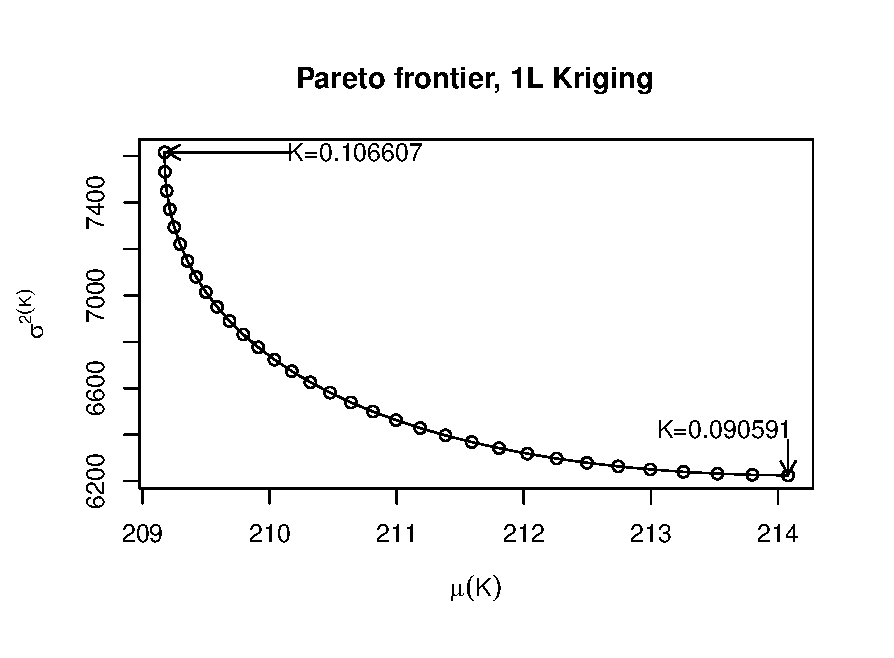
\includegraphics[width = .75\textwidth, height = 0.5\textheight]{pareto_1L} \\
  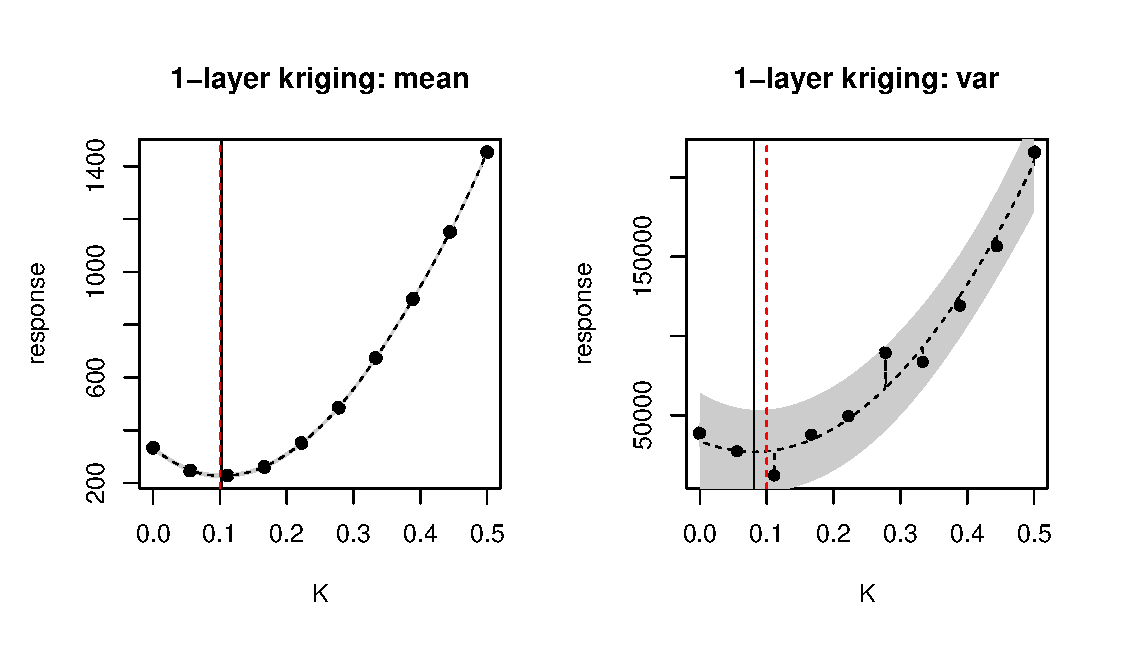
\includegraphics[width = .75\textwidth, height = 0.5\textheight]{mu_sigma_1L}
\end{figure}
}
\frame{
	\frametitle{2L-Kriging}
\scalebox{0.8}{\tikzstyle{block} = [rectangle, draw, fill=blue!20, 
     text centered, rounded corners, minimum width=1cm]

\begin{tikzpicture}[node distance=3cm]
\draw [fill=red!10] (6.2,2) rectangle (12.85,-2) node[below] {\emph{2nd layer}};
\draw [fill=red!10] (1.35,0.8) rectangle (5.3,-0.8) node[below] {\emph{1st layer}};

\node [block] (jfun) {$j$};
% \node [block, right of =jfun] (jfuneval2) {$j(\mathcal{P}_{K_2})$};
% \node [block, above of = jfuneval2] (jfuneval1) {$j(\mathcal{P}_{K_1})$};
% \node [block,below of = jfuneval2] (jfuneval3) {$j(\mathcal{P}_{K_3})$};
\node[block] (jfuneval)  at (2,0) {$j(\mathcal{P})$};
\node [block] (krig1) at (4.3,0) {$\bar{j}(\mathbf{x}_e,K)$};
\node [block] (void2) at (7,0) {$\bar{j}(\mathcal{P}_{2L})$};
\node [block] (mu) at (8.3,1.5){$\{\hat{\mu}_{2L}(K_i)\}_{1 \leq i \leq n_{K,2L}}$};
\node [block] (sigma)at (8.3,-1.5) {$\{\hat{\sigma}^ 2_{2L}(K_i)\}_{1 \leq i \leq n_{K,2L}}$};
\node[block] (mu2L) at (12,1.5) {$\bar{\mu}_{2L}(K)$};
\node[block] (sigma2L) at (12,-1.5)  {$\bar{\sigma}^2_{2L}(K)$};
\node[right of = void2](void3){};
\node[block](pareto) at (14.2,0) {Pareto front};

% \node[block, above of = void1] (muhat){$\{\hat{\mu}(K_i)\}_{1\leq i \leq N_K}$};
% \node[block, right of = jfuneval, below of =jfuneval] (sigmahat){$\{\hat{\sigma}^2(K_i)\}_{1\leq i \leq N_K}$};
% \node[block, right of = muhat](mu1L) {$\bar{\mu}(K)$};
% \node[block, right of = sigmahat](sigma1L) {$\bar{\sigma}^2(K)$};
% \node[block, right of = void2](pareto) {Pareto front};

\draw [->] (jfun) -- (jfuneval) node [above,midway] {LHS};
\draw [->] (jfuneval) -- (krig1) node [above,midway] {Krig.};
% \node at (4.8,0.5) {Krig.};
\draw [->] (krig1) -- (void2)  node [above,midway] {LHS};
\draw [->] (void2) -- (mu);
\draw [->] (void2) -- (sigma);
\draw [->] (mu) -- (mu2L)  node [below,midway] {Krig.};
\draw [->] (sigma) -- (sigma2L)  node [above,midway] {Krig.};
\draw [->] (mu2L) -- (pareto);
\draw [->] (sigma2L) -- (pareto);
% \draw [->] (muhat) -- (mu1L);
% \draw [->] (sigmahat) -- (sigma1L);
% \draw [->] (sigma1L) -- (pareto);
% \draw [->] (mu1L) -- (pareto);

\end{tikzpicture}

}
}
\frame{
\frametitle{2L-Kriging}
\begin{figure}[!h]
  \centering
  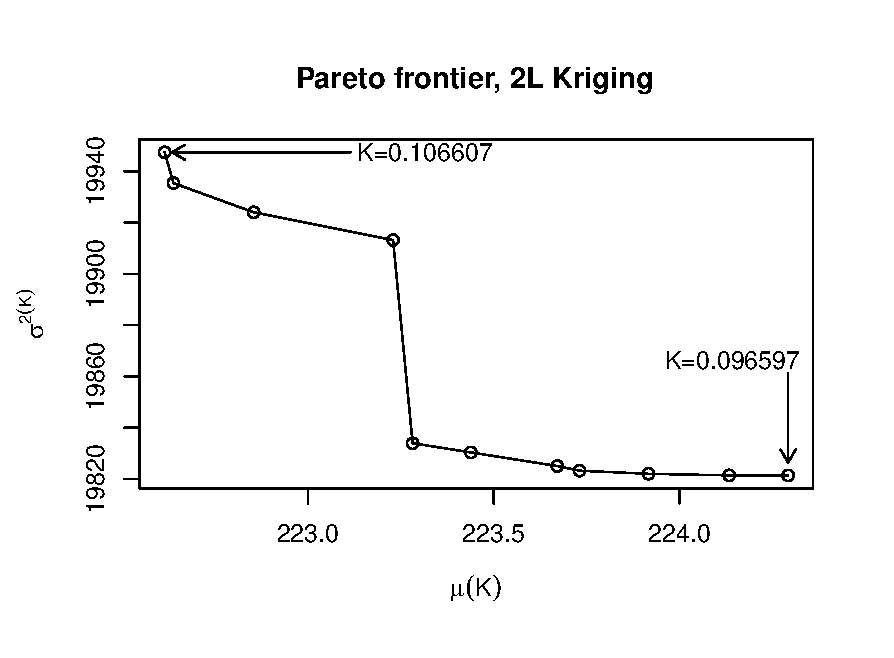
\includegraphics[width = .75\textwidth, height = 0.5\textheight]{Pareto_2L} \\
  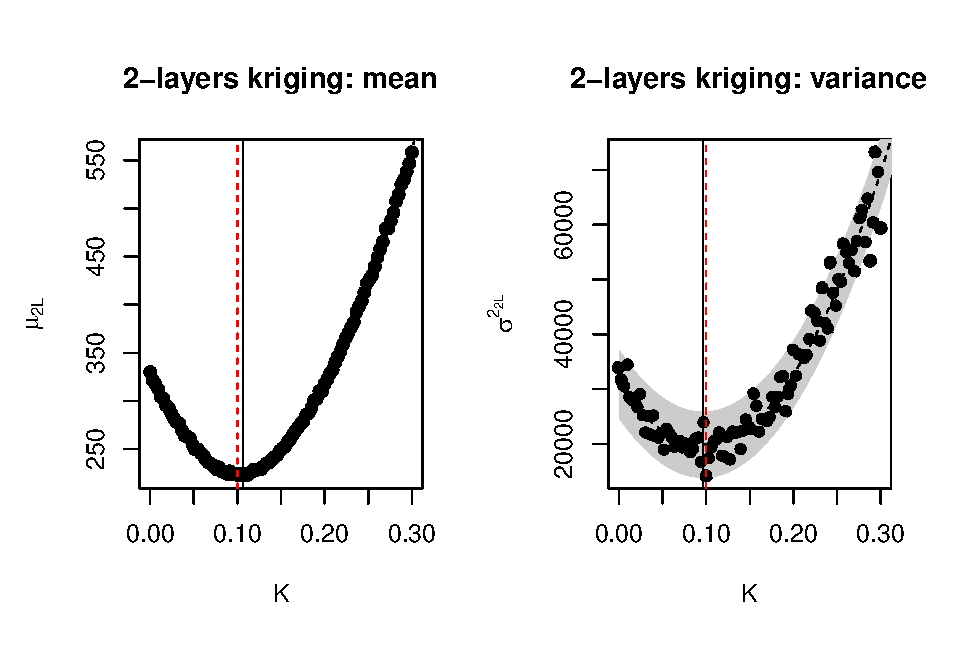
\includegraphics[width = .75\textwidth, height = 0.5\textheight]{mu_sigma_2L}
\end{figure}
}
\subsection*{Steepest descent} 
\frame{
	\frametitle{Steepest descent using PCE \cite{adjointPCE}}
	For a given $K$, expansion of $J(\bm{X}_e,K)$ and $\frac{\partial J}{\partial K}(\bm{X}_e,K)$
	\begin{equation*}
  J(\bm{X}_e,K) = \sum_{\bm{\alpha} \in \mathcal{A}} \hat{J}_{\bm{\alpha}}(K) \Phi_{\bm{\alpha}}(\bm{X}_e)\quad \text{ and }\quad \frac{\partial J}{\partial K}(\bm{X}_e,K) = \sum_{\bm{\alpha} \in \mathcal{A}} \hat{G}_{\bm{\alpha}}(K) \Phi_{\bm{\alpha}}(\bm{X}_e)
  \end{equation*}
  \begin{block}{Relation between $\hat{J}_{\bm{\alpha}}(K)$ and $\hat{G}_{\bm{\alpha}}(K)$}
  \begin{equation*}
  \Rightarrow  \frac{\mathrm{d}\hat{J}_{\bm{\alpha}}}{\mathrm{d}K}(K) = \hat{G}_{\bm{\alpha}}(K),\quad \forall \bm{\alpha} \in \mathcal{A}
\end{equation*}
\end{block}
}

\frame{
\frametitle{Steepest descent using PCE \cite{adjointPCE}}
Recalling that
\begin{equation*}
  \hat{\sigma}^2_J(K) = \sum_{\bm{\alpha} \in \mathcal{A}} \hat{J}_{\bm{\alpha}}(K)^2 \|\Phi_{\bm{\alpha}}\|^2
\end{equation*}
By differentiating with respect to $K$:
\begin{block}{Gradient of the variance}
\begin{equation*}
  \frac{\mathrm{d}\hat{\sigma}^2_J}{\mathrm{d}K}(K) = 2\sum_{\bm{\alpha} \in \mathcal{A}} \hat{J}_{\bm{\alpha}}(K)\frac{\mathrm{d}\hat{J}_{\bm{\alpha}}}{\mathrm{d}K}(K) \|\Phi_{\bm{\alpha}}\|^2 =  2\sum_{\bm{\alpha} \in \mathcal{A}} \hat{J}_{\bm{\alpha}}(K)\hat{G}_{\bm{\alpha}}(K) \|\Phi_{\bm{\alpha}}\|^2 
\end{equation*}
\end{block}
We have the gradient of the mean $\hat{G}_0$ and the gradient of the variance \\ $\Rightarrow$ Gradient descent algorithm.
}

\frame{
\frametitle{Expansion for different $K$}
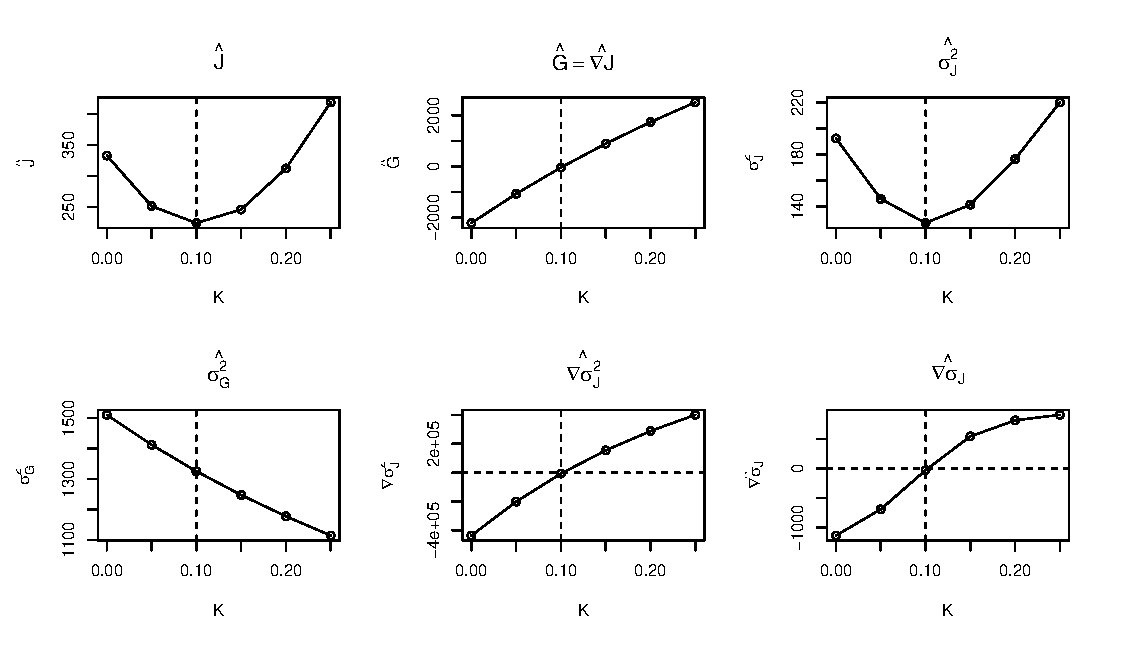
\includegraphics[width = \textwidth]{PCE_CC_43_700x400}
}
\frame{
\frametitle{Gradient descent algorithm on $\rho$}
$\rho(K,\lambda) = \lambda \mu(K) + (1-\lambda)\sigma(K)$
\begin{center}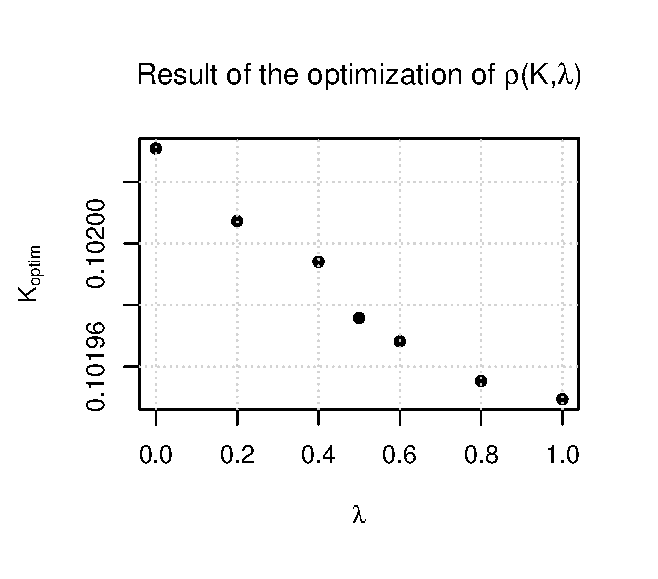
\includegraphics[width = .7\textwidth]{PCE_res_lambda} \end{center}
}

\subsection*{}
%%================================================
%===  Define the contact details
%\newcommand\contactTable{ %
%  \begin{tabular}{lr}
%    \multicolumn{2}{l}{Victor Trappler} \\ 
%    \multicolumn{2}{l}{Inria AIRSEA Intern/future PhD student} \\ \midrule
%    Bâtiment IMAG, Office 195    & s151431@student.dtu.dk. \\
%    St-Martin-d'Hères & +33 645751468 \\
%  \end{tabular}
%}%
%
%\frame[dtuwhitelogo, bgfilename=dtu_bg_fiber]{
%  \begin{tikzpicture}[remember picture,overlay]
%    \node[fill=black, fill opacity=0.9, 
%          text=white, text opacity=1.0,
%          rounded corners=5pt, 
%          font=\scriptsize] at (current page.center) {\contactTable};
%  \end{tikzpicture}
%}
%
%\frame[dtuwhitelogo, bgfilename=dtu_bg_nano]{
%  \begin{tikzpicture}[remember picture,overlay]
%    \node[fill=black, fill opacity=0.9, 
%          text=white, text opacity=1.0,
%          rounded corners=5pt, 
%          font=\scriptsize] at (current page.center) {\contactTable};
%  \end{tikzpicture}
%}
%
%\frame[dtuwhitelogo, bgfilename=dtu_bg_pink]{
%  \begin{tikzpicture}[remember picture,overlay]
%    \node[fill=white, fill opacity=0.8, 
%          text=black, text opacity=1.0,
%          rounded corners=5pt, 
%          font=\scriptsize] at (current page.center) {\contactTable};
%  \end{tikzpicture}
%}
%
\end{document}
